\documentclass[a4paper]{book}
\usepackage{makeidx}
\usepackage{natbib}
\usepackage{graphicx}
\usepackage{multicol}
\usepackage{float}
\usepackage{listings}
\usepackage{color}
\usepackage{ifthen}
\usepackage[table]{xcolor}
\usepackage{textcomp}
\usepackage{alltt}
\usepackage{ifpdf}
\ifpdf
\usepackage[pdftex,
            pagebackref=true,
            colorlinks=true,
            linkcolor=blue,
            unicode
           ]{hyperref}
\else
\usepackage[ps2pdf,
            pagebackref=true,
            colorlinks=true,
            linkcolor=blue,
            unicode
           ]{hyperref}
\usepackage{pspicture}
\fi
\usepackage[utf8]{inputenc}
\usepackage{mathptmx}
\usepackage[scaled=.90]{helvet}
\usepackage{courier}
\usepackage{sectsty}
\usepackage[titles]{tocloft}
\usepackage{doxygen}
\lstset{language=C++,inputencoding=utf8,basicstyle=\footnotesize,breaklines=true,breakatwhitespace=true,tabsize=4,numbers=left }
\makeindex
\setcounter{tocdepth}{3}
\renewcommand{\footrulewidth}{0.4pt}
\renewcommand{\familydefault}{\sfdefault}
\hfuzz=15pt
\setlength{\emergencystretch}{15pt}
\hbadness=750
\tolerance=750
\begin{document}
\hypersetup{pageanchor=false,citecolor=blue}
\begin{titlepage}
\vspace*{7cm}
\begin{center}
{\Large \-C formal concept analysis library }\\
\vspace*{1cm}
{\large \-Generated by Doxygen 1.7.6.1}\\
\vspace*{0.5cm}
{\small Fri Aug 23 2013 12:42:11}\\
\end{center}
\end{titlepage}
\clearemptydoublepage
\pagenumbering{roman}
\tableofcontents
\clearemptydoublepage
\pagenumbering{arabic}
\hypersetup{pageanchor=true,citecolor=blue}
\chapter{\-Data \-Structure \-Index}
\section{\-Data \-Structures}
\-Here are the data structures with brief descriptions\-:\begin{DoxyCompactList}
\item\contentsline{section}{\hyperlink{structsCommutativeProduct}{s\-Commutative\-Product} \\*\-This struct represents a formal product of formal constants x\-\_\-i and their counterparts (1-\/x\-\_\-i) under the assumption of communtativity of the product }{\pageref{structsCommutativeProduct}}{}
\item\contentsline{section}{\hyperlink{structsConditionMap}{s\-Condition\-Map} \\*\-This struct represents a map between the object sets of two formal contexts }{\pageref{structsConditionMap}}{}
\item\contentsline{section}{\hyperlink{structsEtaFunction}{s\-Eta\-Function} \\*\-This structure contains information on how many cases for measurements there are, and what the probabilities of erroneous measurement there is for each case }{\pageref{structsEtaFunction}}{}
\item\contentsline{section}{\hyperlink{structsFormalConceptIntentBulkNode}{s\-Formal\-Concept\-Intent\-Bulk\-Node} \\*\-Node of a single linked list of concept chunks }{\pageref{structsFormalConceptIntentBulkNode}}{}
\item\contentsline{section}{\hyperlink{structsFormalConceptIntentBulkNodeV}{s\-Formal\-Concept\-Intent\-Bulk\-Node\-V} \\*\-Node of a single linked list of concept chunks }{\pageref{structsFormalConceptIntentBulkNodeV}}{}
\item\contentsline{section}{\hyperlink{structsFormalIntent}{s\-Formal\-Intent} \\*\-Intent structure of a formal concept }{\pageref{structsFormalIntent}}{}
\item\contentsline{section}{\hyperlink{structsFormalIntentV}{s\-Formal\-Intent\-V} \\*\-Intent structure of a formal concept }{\pageref{structsFormalIntentV}}{}
\item\contentsline{section}{\hyperlink{structsmyFormalConceptIntentChunk}{smy\-Formal\-Concept\-Intent\-Chunk} \\*\-A chunk of at most \-C\-H\-U\-N\-K\-S\-I\-Z\-E formal concept intents }{\pageref{structsmyFormalConceptIntentChunk}}{}
\item\contentsline{section}{\hyperlink{structsmyFormalConceptIntentChunkV}{smy\-Formal\-Concept\-Intent\-Chunk\-V} \\*\-A chunk of at most \-C\-H\-U\-N\-K\-S\-I\-Z\-E\-V formal concept intent vectors }{\pageref{structsmyFormalConceptIntentChunkV}}{}
\item\contentsline{section}{\hyperlink{structsmyFormalContext}{smy\-Formal\-Context} \\*\-Each formal context has a finite number of objects and attributes, which may have names (though we do not require them to be unique or given), and an incidence relation which is represented by an objects×attributes-\/\-Incidence\-Cell matrix }{\pageref{structsmyFormalContext}}{}
\item\contentsline{section}{\hyperlink{structsmyFormalContextV}{smy\-Formal\-Context\-V} \\*\-Each formal context has a finite number of objects and attributes, which may have names (though we do not require them to be unique or given), and an incidence relation which is represented by an objects×attributes-\/\-Incidence\-Cell matrix }{\pageref{structsmyFormalContextV}}{}
\item\contentsline{section}{\hyperlink{structsnextClosureVX1Params}{snext\-Closure\-V\-X1\-Params} }{\pageref{structsnextClosureVX1Params}}{}
\end{DoxyCompactList}

\chapter{\-File \-Index}
\section{\-File \-List}
\-Here is a list of all files with brief descriptions\-:\begin{DoxyCompactList}
\item\contentsline{section}{src/\hyperlink{cfca_8c}{cfca.\-c} }{\pageref{cfca_8c}}{}
\item\contentsline{section}{src/fca/\hyperlink{common_8h}{common.\-h} }{\pageref{common_8h}}{}
\item\contentsline{section}{src/fca/\hyperlink{easy_8h}{easy.\-h} \\*\-Easy.\-h, (c) 2013, \-Immanuel \-Albrecht; \-Dresden \-University of \-Technology, \-Professur für die \-Psychologie des \-Lernen und \-Lehrens }{\pageref{easy_8h}}{}
\item\contentsline{section}{src/fca/\hyperlink{fca_8h}{fca.\-h} \\*\-Fca.\-h, (c) 2013, \-Immanuel \-Albrecht; \-Dresden \-University of \-Technology, \-Professur für die \-Psychologie des \-Lernen und \-Lehrens }{\pageref{fca_8h}}{}
\item\contentsline{section}{src/fca/\hyperlink{vector_8h}{vector.\-h} \\*\-Vector.\-h, (c) 2013, \-Immanuel \-Albrecht; \-Dresden \-University of \-Technology, \-Professur für die \-Psychologie des \-Lernen und \-Lehrens }{\pageref{vector_8h}}{}
\item\contentsline{section}{src/fca/common/\hyperlink{common_2macros_8h}{macros.\-h} }{\pageref{common_2macros_8h}}{}
\item\contentsline{section}{src/fca/easy/\hyperlink{fca_8c}{fca.\-c} \\*\-Fca.\-c, (c) 2013, \-Immanuel \-Albrecht; \-Dresden \-University of \-Technology, \-Professur für die \-Psychologie des \-Lernen und \-Lehrens }{\pageref{fca_8c}}{}
\item\contentsline{section}{src/fca/easy/\hyperlink{easy_2macros_8h}{macros.\-h} \\*\-Easy/macros.\-h, (c) 2013, \-Immanuel \-Albrecht; \-Dresden \-University of \-Technology, \-Professur für die \-Psychologie des \-Lernen und \-Lehrens }{\pageref{easy_2macros_8h}}{}
\item\contentsline{section}{src/fca/easy/\hyperlink{easy_2private_8h}{private.\-h} }{\pageref{easy_2private_8h}}{}
\item\contentsline{section}{src/fca/easy/\hyperlink{easy_2structs_8h}{structs.\-h} }{\pageref{easy_2structs_8h}}{}
\item\contentsline{section}{src/fca/vector/\hyperlink{fcaV_8c}{fca\-V.\-c} \\*\-Fca\-V.\-c, (c) 2013, \-Immanuel \-Albrecht; \-Dresden \-University of \-Technology, \-Professur für die \-Psychologie des \-Lernen und \-Lehrens }{\pageref{fcaV_8c}}{}
\item\contentsline{section}{src/fca/vector/\hyperlink{fcaVnextClosureX_8c}{fca\-Vnext\-Closure\-X.\-c} \\*\-Fca\-Vnext\-Closure\-X.\-c, (c) 2013, \-Immanuel \-Albrecht; \-Dresden \-University of \-Technology, \-Professur für die \-Psychologie des \-Lernen und \-Lehrens }{\pageref{fcaVnextClosureX_8c}}{}
\item\contentsline{section}{src/fca/vector/\hyperlink{vector_2macros_8h}{macros.\-h} \\*\-Vector/macros.\-h, (c) 2013, \-Immanuel \-Albrecht; \-Dresden \-University of \-Technology, \-Professur für die \-Psychologie des \-Lernen und \-Lehrens }{\pageref{vector_2macros_8h}}{}
\item\contentsline{section}{src/fca/vector/\hyperlink{vector_2private_8h}{private.\-h} }{\pageref{vector_2private_8h}}{}
\item\contentsline{section}{src/fca/vector/\hyperlink{safeguard_8h}{safeguard.\-h} \\*\-Vector/safeguard.\-h, (c) 2013, \-Immanuel \-Albrecht; \-Dresden \-University of \-Technology, \-Professur für die \-Psychologie des \-Lernen und \-Lehrens }{\pageref{safeguard_8h}}{}
\item\contentsline{section}{src/fca/vector/\hyperlink{vector_2structs_8h}{structs.\-h} }{\pageref{vector_2structs_8h}}{}
\end{DoxyCompactList}

\chapter{\-Data \-Structure \-Documentation}
\hypertarget{structsCommutativeProduct}{\section{s\-Commutative\-Product \-Struct \-Reference}
\label{structsCommutativeProduct}\index{s\-Commutative\-Product@{s\-Commutative\-Product}}
}


\-This struct represents a formal product of formal constants x\-\_\-i and their counterparts (1-\/x\-\_\-i) under the assumption of communtativity of the product.  




{\ttfamily \#include $<$measurement.\-h$>$}

\subsection*{\-Data \-Fields}
\begin{DoxyCompactItemize}
\item 
size\-\_\-t \hyperlink{structsCommutativeProduct_af77351b19630473b2fedc9267665032a}{constants}
\begin{DoxyCompactList}\small\item\em the number of different formal probability constants \end{DoxyCompactList}\item 
size\-\_\-t $\ast$ \hyperlink{structsCommutativeProduct_a95aa7c0ea80854b88afc16d913137f35}{mismatch}
\begin{DoxyCompactList}\small\item\em \-This represents the first term part. \end{DoxyCompactList}\item 
size\-\_\-t $\ast$ \hyperlink{structsCommutativeProduct_ae78261dbaf0a6455774a84836fe7334d}{match}
\begin{DoxyCompactList}\small\item\em \-The represents the second term part. \end{DoxyCompactList}\item 
\hyperlink{common_2measurement_8h_a0a02860cc83aa9ce63d00855bc9058e0}{\-Log\-Probability} $\ast$ \hyperlink{structsCommutativeProduct_a62301df4ed7d412fb3e45fc7f8d6b0f3}{intermediate}
\begin{DoxyCompactList}\small\item\em \-This is an intermediate helper structure used to calculate the log probabilities\-: we need to store the intermediate results per constant and matchtype. \end{DoxyCompactList}\end{DoxyCompactItemize}


\subsection{\-Detailed \-Description}
\-This struct represents a formal product of formal constants x\-\_\-i and their counterparts (1-\/x\-\_\-i) under the assumption of communtativity of the product. 

\-E.\-g.

\[ \prod_{i=0}^{\mathrm{constants}} x_i^{\mathrm{mismatch}(i)} \cdot (1-x_i)^{\mathrm{match}(i)} \] 

\-Definition at line 101 of file measurement.\-h.



\subsection{\-Field \-Documentation}
\hypertarget{structsCommutativeProduct_af77351b19630473b2fedc9267665032a}{\index{s\-Commutative\-Product@{s\-Commutative\-Product}!constants@{constants}}
\index{constants@{constants}!sCommutativeProduct@{s\-Commutative\-Product}}
\subsubsection[{constants}]{\setlength{\rightskip}{0pt plus 5cm}size\-\_\-t {\bf s\-Commutative\-Product\-::constants}}}\label{structsCommutativeProduct_af77351b19630473b2fedc9267665032a}


the number of different formal probability constants 



\-Definition at line 106 of file measurement.\-h.



\-Referenced by calculate\-Likelihood(), log\-Probability\-From\-Product(), and new\-Commutative\-Product().

\hypertarget{structsCommutativeProduct_a62301df4ed7d412fb3e45fc7f8d6b0f3}{\index{s\-Commutative\-Product@{s\-Commutative\-Product}!intermediate@{intermediate}}
\index{intermediate@{intermediate}!sCommutativeProduct@{s\-Commutative\-Product}}
\subsubsection[{intermediate}]{\setlength{\rightskip}{0pt plus 5cm}{\bf \-Log\-Probability}$\ast$ {\bf s\-Commutative\-Product\-::intermediate}}}\label{structsCommutativeProduct_a62301df4ed7d412fb3e45fc7f8d6b0f3}


\-This is an intermediate helper structure used to calculate the log probabilities\-: we need to store the intermediate results per constant and matchtype. 

\-Length of this array\-: 2$\ast$constants 

\-Definition at line 126 of file measurement.\-h.



\-Referenced by log\-Probability\-From\-Product(), and new\-Commutative\-Product().

\hypertarget{structsCommutativeProduct_ae78261dbaf0a6455774a84836fe7334d}{\index{s\-Commutative\-Product@{s\-Commutative\-Product}!match@{match}}
\index{match@{match}!sCommutativeProduct@{s\-Commutative\-Product}}
\subsubsection[{match}]{\setlength{\rightskip}{0pt plus 5cm}size\-\_\-t$\ast$ {\bf s\-Commutative\-Product\-::match}}}\label{structsCommutativeProduct_ae78261dbaf0a6455774a84836fe7334d}


\-The represents the second term part. 

\[ \prod_{i=0}^{\mathrm{constants}} (1-x_i)^{\mathrm{match}(i)} \] 

\-Definition at line 118 of file measurement.\-h.



\-Referenced by calculate\-Likelihood(), log\-Probability\-From\-Product(), new\-Commutative\-Product(), and new\-Distance\-Matrix\-From\-Context().

\hypertarget{structsCommutativeProduct_a95aa7c0ea80854b88afc16d913137f35}{\index{s\-Commutative\-Product@{s\-Commutative\-Product}!mismatch@{mismatch}}
\index{mismatch@{mismatch}!sCommutativeProduct@{s\-Commutative\-Product}}
\subsubsection[{mismatch}]{\setlength{\rightskip}{0pt plus 5cm}size\-\_\-t$\ast$ {\bf s\-Commutative\-Product\-::mismatch}}}\label{structsCommutativeProduct_a95aa7c0ea80854b88afc16d913137f35}


\-This represents the first term part. 

\[ \prod_{i=0}^{\mathrm{constants}} x_i^{\mathrm{mismatch}(i)} \] 

\-Definition at line 112 of file measurement.\-h.



\-Referenced by calculate\-Likelihood(), log\-Probability\-From\-Product(), new\-Commutative\-Product(), and new\-Distance\-Matrix\-From\-Context().



\-The documentation for this struct was generated from the following file\-:\begin{DoxyCompactItemize}
\item 
src/fca/common/\hyperlink{common_2measurement_8h}{measurement.\-h}\end{DoxyCompactItemize}

\hypertarget{structsConditionMap}{\section{s\-Condition\-Map \-Struct \-Reference}
\label{structsConditionMap}\index{s\-Condition\-Map@{s\-Condition\-Map}}
}


\-This struct represents a map between the object sets of two formal contexts.  




{\ttfamily \#include $<$measurement.\-h$>$}

\subsection*{\-Data \-Fields}
\begin{DoxyCompactItemize}
\item 
size\-\_\-t \hyperlink{structsConditionMap_a6a6975dfaba87cd345610cf6526ede4e}{attributes}
\begin{DoxyCompactList}\small\item\em number of attributes in the domain object set \end{DoxyCompactList}\item 
size\-\_\-t $\ast$ \hyperlink{structsConditionMap_a8fba8e129aa41cc4fd2f1898e83c2f28}{c}
\begin{DoxyCompactList}\small\item\em the attribute index of the image, i.\-e. \end{DoxyCompactList}\end{DoxyCompactItemize}


\subsection{\-Detailed \-Description}
\-This struct represents a map between the object sets of two formal contexts. 

\-Definition at line 120 of file measurement.\-h.



\subsection{\-Field \-Documentation}
\hypertarget{structsConditionMap_a6a6975dfaba87cd345610cf6526ede4e}{\index{s\-Condition\-Map@{s\-Condition\-Map}!attributes@{attributes}}
\index{attributes@{attributes}!sConditionMap@{s\-Condition\-Map}}
\subsubsection[{attributes}]{\setlength{\rightskip}{0pt plus 5cm}size\-\_\-t {\bf s\-Condition\-Map\-::attributes}}}\label{structsConditionMap_a6a6975dfaba87cd345610cf6526ede4e}


number of attributes in the domain object set 



\-Definition at line 124 of file measurement.\-h.



\-Referenced by new\-Condition\-Map().

\hypertarget{structsConditionMap_a8fba8e129aa41cc4fd2f1898e83c2f28}{\index{s\-Condition\-Map@{s\-Condition\-Map}!c@{c}}
\index{c@{c}!sConditionMap@{s\-Condition\-Map}}
\subsubsection[{c}]{\setlength{\rightskip}{0pt plus 5cm}size\-\_\-t$\ast$ {\bf s\-Condition\-Map\-::c}}}\label{structsConditionMap_a8fba8e129aa41cc4fd2f1898e83c2f28}


the attribute index of the image, i.\-e. 

c\mbox{[}i\mbox{]} is the index of the image of the attribute with index i in the domain 

\-Definition at line 130 of file measurement.\-h.



\-Referenced by new\-Condition\-Map().



\-The documentation for this struct was generated from the following file\-:\begin{DoxyCompactItemize}
\item 
src/fca/common/\hyperlink{common_2measurement_8h}{measurement.\-h}\end{DoxyCompactItemize}

\hypertarget{structsEtaFunction}{\section{s\-Eta\-Function \-Struct \-Reference}
\label{structsEtaFunction}\index{s\-Eta\-Function@{s\-Eta\-Function}}
}


this structure contains information on how many cases for measurements there are, and what the probabilities of erroneous measurement there is for each case  




{\ttfamily \#include $<$measurement.\-h$>$}

\subsection*{\-Data \-Fields}
\begin{DoxyCompactItemize}
\item 
size\-\_\-t \hyperlink{structsEtaFunction_a1fdf63f3a73e7fd663491e72421619f9}{constants}
\begin{DoxyCompactList}\small\item\em the number of different probability constants \end{DoxyCompactList}\item 
\hyperlink{measurement_8h_ae6d7a8c80f18bc080ab1cfa38d119724}{\-Probability} $\ast$ \hyperlink{structsEtaFunction_a05c2f93c1148d5268d359d78540c10be}{\-C}
\begin{DoxyCompactList}\small\item\em the constants array. \end{DoxyCompactList}\item 
size\-\_\-t \hyperlink{structsEtaFunction_afd94a9856047e0987c5e8667a4838b71}{types}
\begin{DoxyCompactList}\small\item\em the number of error types \end{DoxyCompactList}\item 
size\-\_\-t \hyperlink{structsEtaFunction_aa323ef11935cd1e8d6ef56405ab96cf8}{measurements}
\begin{DoxyCompactList}\small\item\em the number of different measurements \end{DoxyCompactList}\item 
size\-\_\-t $\ast$ \hyperlink{structsEtaFunction_a7585a59b1861523157055f8c8b0263e3}{eta}
\begin{DoxyCompactList}\small\item\em the error constants, where the rows (t) are types, and the columns (m) are measurements, i.\-e. \end{DoxyCompactList}\end{DoxyCompactItemize}


\subsection{\-Detailed \-Description}
this structure contains information on how many cases for measurements there are, and what the probabilities of erroneous measurement there is for each case 

\-Definition at line 34 of file measurement.\-h.



\subsection{\-Field \-Documentation}
\hypertarget{structsEtaFunction_a05c2f93c1148d5268d359d78540c10be}{\index{s\-Eta\-Function@{s\-Eta\-Function}!\-C@{\-C}}
\index{\-C@{\-C}!sEtaFunction@{s\-Eta\-Function}}
\subsubsection[{\-C}]{\setlength{\rightskip}{0pt plus 5cm}{\bf \-Probability}$\ast$ {\bf s\-Eta\-Function\-::\-C}}}\label{structsEtaFunction_a05c2f93c1148d5268d359d78540c10be}


the constants array. 



\-Definition at line 44 of file measurement.\-h.



\-Referenced by new\-Eta\-Function().

\hypertarget{structsEtaFunction_a1fdf63f3a73e7fd663491e72421619f9}{\index{s\-Eta\-Function@{s\-Eta\-Function}!constants@{constants}}
\index{constants@{constants}!sEtaFunction@{s\-Eta\-Function}}
\subsubsection[{constants}]{\setlength{\rightskip}{0pt plus 5cm}size\-\_\-t {\bf s\-Eta\-Function\-::constants}}}\label{structsEtaFunction_a1fdf63f3a73e7fd663491e72421619f9}


the number of different probability constants 



\-Definition at line 38 of file measurement.\-h.



\-Referenced by new\-Eta\-Function().

\hypertarget{structsEtaFunction_a7585a59b1861523157055f8c8b0263e3}{\index{s\-Eta\-Function@{s\-Eta\-Function}!eta@{eta}}
\index{eta@{eta}!sEtaFunction@{s\-Eta\-Function}}
\subsubsection[{eta}]{\setlength{\rightskip}{0pt plus 5cm}size\-\_\-t$\ast$ {\bf s\-Eta\-Function\-::eta}}}\label{structsEtaFunction_a7585a59b1861523157055f8c8b0263e3}


the error constants, where the rows (t) are types, and the columns (m) are measurements, i.\-e. 

the error probability for type t error and measurement m is\-:

\-C\mbox{[}eta\mbox{[}t$\ast$measurements + m\mbox{]}\mbox{]} 

\-Definition at line 64 of file measurement.\-h.



\-Referenced by new\-Eta\-Function().

\hypertarget{structsEtaFunction_aa323ef11935cd1e8d6ef56405ab96cf8}{\index{s\-Eta\-Function@{s\-Eta\-Function}!measurements@{measurements}}
\index{measurements@{measurements}!sEtaFunction@{s\-Eta\-Function}}
\subsubsection[{measurements}]{\setlength{\rightskip}{0pt plus 5cm}size\-\_\-t {\bf s\-Eta\-Function\-::measurements}}}\label{structsEtaFunction_aa323ef11935cd1e8d6ef56405ab96cf8}


the number of different measurements 



\-Definition at line 55 of file measurement.\-h.



\-Referenced by new\-Eta\-Function().

\hypertarget{structsEtaFunction_afd94a9856047e0987c5e8667a4838b71}{\index{s\-Eta\-Function@{s\-Eta\-Function}!types@{types}}
\index{types@{types}!sEtaFunction@{s\-Eta\-Function}}
\subsubsection[{types}]{\setlength{\rightskip}{0pt plus 5cm}size\-\_\-t {\bf s\-Eta\-Function\-::types}}}\label{structsEtaFunction_afd94a9856047e0987c5e8667a4838b71}


the number of error types 



\-Definition at line 49 of file measurement.\-h.



\-Referenced by new\-Eta\-Function().



\-The documentation for this struct was generated from the following file\-:\begin{DoxyCompactItemize}
\item 
src/fca/common/\hyperlink{measurement_8h}{measurement.\-h}\end{DoxyCompactItemize}

\hypertarget{structsFormalConceptIntentBulkNode}{\section{s\-Formal\-Concept\-Intent\-Bulk\-Node \-Struct \-Reference}
\label{structsFormalConceptIntentBulkNode}\index{s\-Formal\-Concept\-Intent\-Bulk\-Node@{s\-Formal\-Concept\-Intent\-Bulk\-Node}}
}


a node of a single linked list of concept chunks.  




{\ttfamily \#include $<$structs.\-h$>$}



\-Collaboration diagram for s\-Formal\-Concept\-Intent\-Bulk\-Node\-:\nopagebreak
\begin{figure}[H]
\begin{center}
\leavevmode
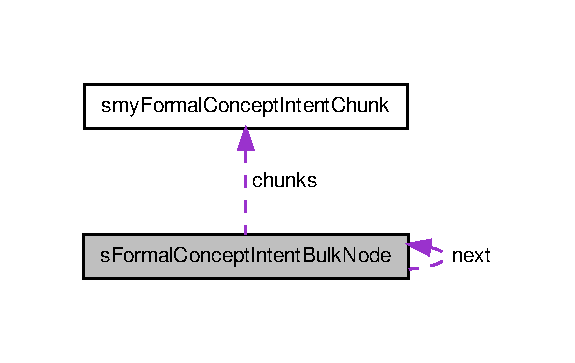
\includegraphics[width=276pt]{structsFormalConceptIntentBulkNode__coll__graph}
\end{center}
\end{figure}
\subsection*{\-Data \-Fields}
\begin{DoxyCompactItemize}
\item 
int \hyperlink{structsFormalConceptIntentBulkNode_a1fbfa6da3820560fef8549991a83e694}{attributes}
\begin{DoxyCompactList}\small\item\em number of attributes of the concept intents \end{DoxyCompactList}\item 
int \hyperlink{structsFormalConceptIntentBulkNode_afc96b660c7becf5517e4391846e0975f}{size}
\begin{DoxyCompactList}\small\item\em number of chunks used \end{DoxyCompactList}\item 
\hyperlink{easy_2structs_8h_ae552e1b13988c8c4ca0ab8f8a3e60f96}{my\-Formal\-Concept\-Intent\-Chunk} $\ast$$\ast$ \hyperlink{structsFormalConceptIntentBulkNode_a581d8ff2f4deebf047730cfd5be1f754}{chunks}
\begin{DoxyCompactList}\small\item\em array to at most \-B\-U\-L\-K\-S\-I\-Z\-E chunks \end{DoxyCompactList}\item 
struct \*
\hyperlink{structsFormalConceptIntentBulkNode}{s\-Formal\-Concept\-Intent\-Bulk\-Node} $\ast$ \hyperlink{structsFormalConceptIntentBulkNode_a1cff65c57653d96d207878be8614b383}{next}
\begin{DoxyCompactList}\small\item\em pointer to the next \-Bulk\-Node, or 0 \end{DoxyCompactList}\end{DoxyCompactItemize}


\subsection{\-Detailed \-Description}
a node of a single linked list of concept chunks. 

bulk nodes are filled chunk wise, but a bulk node may have non-\/empty successor nodes even if it is not entire full. 

\-Definition at line 89 of file structs.\-h.



\subsection{\-Field \-Documentation}
\hypertarget{structsFormalConceptIntentBulkNode_a1fbfa6da3820560fef8549991a83e694}{\index{s\-Formal\-Concept\-Intent\-Bulk\-Node@{s\-Formal\-Concept\-Intent\-Bulk\-Node}!attributes@{attributes}}
\index{attributes@{attributes}!sFormalConceptIntentBulkNode@{s\-Formal\-Concept\-Intent\-Bulk\-Node}}
\subsubsection[{attributes}]{\setlength{\rightskip}{0pt plus 5cm}int {\bf s\-Formal\-Concept\-Intent\-Bulk\-Node\-::attributes}}}\label{structsFormalConceptIntentBulkNode_a1fbfa6da3820560fef8549991a83e694}


number of attributes of the concept intents 



\-Definition at line 94 of file structs.\-h.



\-Referenced by add\-Concept\-To\-Bulk(), new\-Concept\-Bulk(), and write\-Concepts\-To\-File().

\hypertarget{structsFormalConceptIntentBulkNode_a581d8ff2f4deebf047730cfd5be1f754}{\index{s\-Formal\-Concept\-Intent\-Bulk\-Node@{s\-Formal\-Concept\-Intent\-Bulk\-Node}!chunks@{chunks}}
\index{chunks@{chunks}!sFormalConceptIntentBulkNode@{s\-Formal\-Concept\-Intent\-Bulk\-Node}}
\subsubsection[{chunks}]{\setlength{\rightskip}{0pt plus 5cm}{\bf my\-Formal\-Concept\-Intent\-Chunk}$\ast$$\ast$ {\bf s\-Formal\-Concept\-Intent\-Bulk\-Node\-::chunks}}}\label{structsFormalConceptIntentBulkNode_a581d8ff2f4deebf047730cfd5be1f754}


array to at most \-B\-U\-L\-K\-S\-I\-Z\-E chunks 



\-Definition at line 102 of file structs.\-h.



\-Referenced by add\-Concept\-To\-Bulk(), count\-Concepts\-In\-Bulk(), delete\-Concept\-Bulk(), new\-Concept\-Bulk(), and write\-Concepts\-To\-File().

\hypertarget{structsFormalConceptIntentBulkNode_a1cff65c57653d96d207878be8614b383}{\index{s\-Formal\-Concept\-Intent\-Bulk\-Node@{s\-Formal\-Concept\-Intent\-Bulk\-Node}!next@{next}}
\index{next@{next}!sFormalConceptIntentBulkNode@{s\-Formal\-Concept\-Intent\-Bulk\-Node}}
\subsubsection[{next}]{\setlength{\rightskip}{0pt plus 5cm}struct {\bf s\-Formal\-Concept\-Intent\-Bulk\-Node}$\ast$ {\bf s\-Formal\-Concept\-Intent\-Bulk\-Node\-::next}}}\label{structsFormalConceptIntentBulkNode_a1cff65c57653d96d207878be8614b383}


pointer to the next \-Bulk\-Node, or 0 



\-Definition at line 106 of file structs.\-h.



\-Referenced by add\-Concept\-To\-Bulk(), count\-Concepts\-In\-Bulk(), delete\-Concept\-Bulk(), new\-Concept\-Bulk(), and write\-Concepts\-To\-File().

\hypertarget{structsFormalConceptIntentBulkNode_afc96b660c7becf5517e4391846e0975f}{\index{s\-Formal\-Concept\-Intent\-Bulk\-Node@{s\-Formal\-Concept\-Intent\-Bulk\-Node}!size@{size}}
\index{size@{size}!sFormalConceptIntentBulkNode@{s\-Formal\-Concept\-Intent\-Bulk\-Node}}
\subsubsection[{size}]{\setlength{\rightskip}{0pt plus 5cm}int {\bf s\-Formal\-Concept\-Intent\-Bulk\-Node\-::size}}}\label{structsFormalConceptIntentBulkNode_afc96b660c7becf5517e4391846e0975f}


number of chunks used 



\-Definition at line 98 of file structs.\-h.



\-Referenced by add\-Concept\-To\-Bulk(), count\-Concepts\-In\-Bulk(), delete\-Concept\-Bulk(), new\-Concept\-Bulk(), and write\-Concepts\-To\-File().



\-The documentation for this struct was generated from the following file\-:\begin{DoxyCompactItemize}
\item 
src/fca/easy/\hyperlink{easy_2structs_8h}{structs.\-h}\end{DoxyCompactItemize}

\hypertarget{structsFormalConceptIntentBulkNodeV}{\section{s\-Formal\-Concept\-Intent\-Bulk\-Node\-V \-Struct \-Reference}
\label{structsFormalConceptIntentBulkNodeV}\index{s\-Formal\-Concept\-Intent\-Bulk\-Node\-V@{s\-Formal\-Concept\-Intent\-Bulk\-Node\-V}}
}


a node of a single linked list of concept chunks.  




{\ttfamily \#include $<$structs.\-h$>$}



\-Collaboration diagram for s\-Formal\-Concept\-Intent\-Bulk\-Node\-V\-:\nopagebreak
\begin{figure}[H]
\begin{center}
\leavevmode
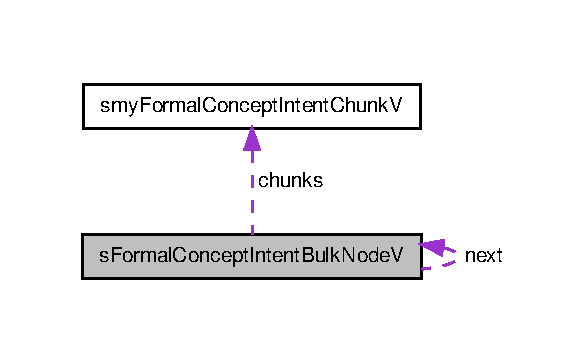
\includegraphics[width=282pt]{structsFormalConceptIntentBulkNodeV__coll__graph}
\end{center}
\end{figure}
\subsection*{\-Data \-Fields}
\begin{DoxyCompactItemize}
\item 
size\-\_\-t \hyperlink{structsFormalConceptIntentBulkNodeV_a0bcc56cc39eb49a954c136099d6e46e7}{attributes}
\begin{DoxyCompactList}\small\item\em number of attributes of the concept intents \end{DoxyCompactList}\item 
size\-\_\-t \hyperlink{structsFormalConceptIntentBulkNodeV_ab6c271021365b30649e33b474862f5d8}{width}
\begin{DoxyCompactList}\small\item\em width of each attribute vector \end{DoxyCompactList}\item 
size\-\_\-t \hyperlink{structsFormalConceptIntentBulkNodeV_a516403c9da58b5bedbf72f0a037d5c4f}{size}
\begin{DoxyCompactList}\small\item\em number of chunks used \end{DoxyCompactList}\item 
\hyperlink{vector_2structs_8h_abe3c190ec3375121cbfe3afff517b9b9}{my\-Formal\-Concept\-Intent\-Chunk\-V} $\ast$$\ast$ \hyperlink{structsFormalConceptIntentBulkNodeV_a0e2dad46489f048d39181e59eb1c6039}{chunks}
\begin{DoxyCompactList}\small\item\em array to at most \-B\-U\-L\-K\-S\-I\-Z\-E\-V chunks \end{DoxyCompactList}\item 
struct \*
\hyperlink{structsFormalConceptIntentBulkNodeV}{s\-Formal\-Concept\-Intent\-Bulk\-Node\-V} $\ast$ \hyperlink{structsFormalConceptIntentBulkNodeV_ac2cd46a8c3334e2d2fdbc6c203707ed8}{next}
\begin{DoxyCompactList}\small\item\em pointer to the next \-Bulk\-Node, or 0 \end{DoxyCompactList}\end{DoxyCompactItemize}


\subsection{\-Detailed \-Description}
a node of a single linked list of concept chunks. 

bulk nodes are filled chunk wise, but a bulk node may have non-\/empty successor nodes even if it is not entire full. 

\-Definition at line 93 of file structs.\-h.



\subsection{\-Field \-Documentation}
\hypertarget{structsFormalConceptIntentBulkNodeV_a0bcc56cc39eb49a954c136099d6e46e7}{\index{s\-Formal\-Concept\-Intent\-Bulk\-Node\-V@{s\-Formal\-Concept\-Intent\-Bulk\-Node\-V}!attributes@{attributes}}
\index{attributes@{attributes}!sFormalConceptIntentBulkNodeV@{s\-Formal\-Concept\-Intent\-Bulk\-Node\-V}}
\subsubsection[{attributes}]{\setlength{\rightskip}{0pt plus 5cm}size\-\_\-t {\bf s\-Formal\-Concept\-Intent\-Bulk\-Node\-V\-::attributes}}}\label{structsFormalConceptIntentBulkNodeV_a0bcc56cc39eb49a954c136099d6e46e7}


number of attributes of the concept intents 



\-Definition at line 98 of file structs.\-h.



\-Referenced by add\-Concept\-To\-Bulk\-V(), new\-Concept\-Bulk\-V(), and write\-Concepts\-To\-File\-V().

\hypertarget{structsFormalConceptIntentBulkNodeV_a0e2dad46489f048d39181e59eb1c6039}{\index{s\-Formal\-Concept\-Intent\-Bulk\-Node\-V@{s\-Formal\-Concept\-Intent\-Bulk\-Node\-V}!chunks@{chunks}}
\index{chunks@{chunks}!sFormalConceptIntentBulkNodeV@{s\-Formal\-Concept\-Intent\-Bulk\-Node\-V}}
\subsubsection[{chunks}]{\setlength{\rightskip}{0pt plus 5cm}{\bf my\-Formal\-Concept\-Intent\-Chunk\-V}$\ast$$\ast$ {\bf s\-Formal\-Concept\-Intent\-Bulk\-Node\-V\-::chunks}}}\label{structsFormalConceptIntentBulkNodeV_a0e2dad46489f048d39181e59eb1c6039}


array to at most \-B\-U\-L\-K\-S\-I\-Z\-E\-V chunks 



\-Definition at line 110 of file structs.\-h.



\-Referenced by add\-Concept\-To\-Bulk\-V(), count\-Concepts\-In\-Bulk\-V(), delete\-Concept\-Bulk\-V(), new\-Concept\-Bulk\-V(), and write\-Concepts\-To\-File\-V().

\hypertarget{structsFormalConceptIntentBulkNodeV_ac2cd46a8c3334e2d2fdbc6c203707ed8}{\index{s\-Formal\-Concept\-Intent\-Bulk\-Node\-V@{s\-Formal\-Concept\-Intent\-Bulk\-Node\-V}!next@{next}}
\index{next@{next}!sFormalConceptIntentBulkNodeV@{s\-Formal\-Concept\-Intent\-Bulk\-Node\-V}}
\subsubsection[{next}]{\setlength{\rightskip}{0pt plus 5cm}struct {\bf s\-Formal\-Concept\-Intent\-Bulk\-Node\-V}$\ast$ {\bf s\-Formal\-Concept\-Intent\-Bulk\-Node\-V\-::next}}}\label{structsFormalConceptIntentBulkNodeV_ac2cd46a8c3334e2d2fdbc6c203707ed8}


pointer to the next \-Bulk\-Node, or 0 



\-Definition at line 114 of file structs.\-h.



\-Referenced by add\-Concept\-To\-Bulk\-V(), count\-Concepts\-In\-Bulk\-V(), delete\-Concept\-Bulk\-V(), new\-Concept\-Bulk\-V(), next\-Closure\-V\-X(), and write\-Concepts\-To\-File\-V().

\hypertarget{structsFormalConceptIntentBulkNodeV_a516403c9da58b5bedbf72f0a037d5c4f}{\index{s\-Formal\-Concept\-Intent\-Bulk\-Node\-V@{s\-Formal\-Concept\-Intent\-Bulk\-Node\-V}!size@{size}}
\index{size@{size}!sFormalConceptIntentBulkNodeV@{s\-Formal\-Concept\-Intent\-Bulk\-Node\-V}}
\subsubsection[{size}]{\setlength{\rightskip}{0pt plus 5cm}size\-\_\-t {\bf s\-Formal\-Concept\-Intent\-Bulk\-Node\-V\-::size}}}\label{structsFormalConceptIntentBulkNodeV_a516403c9da58b5bedbf72f0a037d5c4f}


number of chunks used 



\-Definition at line 106 of file structs.\-h.



\-Referenced by add\-Concept\-To\-Bulk\-V(), count\-Concepts\-In\-Bulk\-V(), delete\-Concept\-Bulk\-V(), new\-Concept\-Bulk\-V(), and write\-Concepts\-To\-File\-V().

\hypertarget{structsFormalConceptIntentBulkNodeV_ab6c271021365b30649e33b474862f5d8}{\index{s\-Formal\-Concept\-Intent\-Bulk\-Node\-V@{s\-Formal\-Concept\-Intent\-Bulk\-Node\-V}!width@{width}}
\index{width@{width}!sFormalConceptIntentBulkNodeV@{s\-Formal\-Concept\-Intent\-Bulk\-Node\-V}}
\subsubsection[{width}]{\setlength{\rightskip}{0pt plus 5cm}size\-\_\-t {\bf s\-Formal\-Concept\-Intent\-Bulk\-Node\-V\-::width}}}\label{structsFormalConceptIntentBulkNodeV_ab6c271021365b30649e33b474862f5d8}


width of each attribute vector 



\-Definition at line 102 of file structs.\-h.



\-Referenced by add\-Concept\-To\-Bulk\-V(), and new\-Concept\-Bulk\-V().



\-The documentation for this struct was generated from the following file\-:\begin{DoxyCompactItemize}
\item 
src/fca/vector/\hyperlink{vector_2structs_8h}{structs.\-h}\end{DoxyCompactItemize}

\hypertarget{structsFormalIntent}{\section{s\-Formal\-Intent \-Struct \-Reference}
\label{structsFormalIntent}\index{s\-Formal\-Intent@{s\-Formal\-Intent}}
}


intent structure of a formal concept  




{\ttfamily \#include $<$easy.\-h$>$}

\subsection*{\-Data \-Fields}
\begin{DoxyCompactItemize}
\item 
size\-\_\-t \hyperlink{structsFormalIntent_a74e2f2885fae7bdfe1ecf1b3a161d625}{attributes}
\item 
\hyperlink{easy_8h_a92fa84ef7a12663bb998f141ab729056}{\-Incidence\-Cell} $\ast$ \hyperlink{structsFormalIntent_a81eeab9acf7444b47416e4b72dea0462}{incidence}
\end{DoxyCompactItemize}


\subsection{\-Detailed \-Description}
intent structure of a formal concept 

\-Definition at line 48 of file easy.\-h.



\subsection{\-Field \-Documentation}
\hypertarget{structsFormalIntent_a74e2f2885fae7bdfe1ecf1b3a161d625}{\index{s\-Formal\-Intent@{s\-Formal\-Intent}!attributes@{attributes}}
\index{attributes@{attributes}!sFormalIntent@{s\-Formal\-Intent}}
\subsubsection[{attributes}]{\setlength{\rightskip}{0pt plus 5cm}size\-\_\-t {\bf s\-Formal\-Intent\-::attributes}}}\label{structsFormalIntent_a74e2f2885fae7bdfe1ecf1b3a161d625}


\-Definition at line 50 of file easy.\-h.

\hypertarget{structsFormalIntent_a81eeab9acf7444b47416e4b72dea0462}{\index{s\-Formal\-Intent@{s\-Formal\-Intent}!incidence@{incidence}}
\index{incidence@{incidence}!sFormalIntent@{s\-Formal\-Intent}}
\subsubsection[{incidence}]{\setlength{\rightskip}{0pt plus 5cm}{\bf \-Incidence\-Cell}$\ast$ {\bf s\-Formal\-Intent\-::incidence}}}\label{structsFormalIntent_a81eeab9acf7444b47416e4b72dea0462}


\-Definition at line 51 of file easy.\-h.



\-The documentation for this struct was generated from the following file\-:\begin{DoxyCompactItemize}
\item 
src/fca/\hyperlink{easy_8h}{easy.\-h}\end{DoxyCompactItemize}

\hypertarget{structsFormalIntentV}{\section{s\-Formal\-Intent\-V \-Struct \-Reference}
\label{structsFormalIntentV}\index{s\-Formal\-Intent\-V@{s\-Formal\-Intent\-V}}
}


intent structure of a formal concept  




{\ttfamily \#include $<$vector.\-h$>$}

\subsection*{\-Data \-Fields}
\begin{DoxyCompactItemize}
\item 
size\-\_\-t \hyperlink{structsFormalIntentV_addf2a15164915bd6dbc77d4ff48325de}{attributes}
\begin{DoxyCompactList}\small\item\em nbr of attributes in this vector \end{DoxyCompactList}\item 
size\-\_\-t \hyperlink{structsFormalIntentV_a70711ba6edc09660adb6a838ef8d1555}{width}
\begin{DoxyCompactList}\small\item\em the width, i.\-e. \end{DoxyCompactList}\item 
\hyperlink{vector_8h_aae617489ac88fff15979050721fe581f}{\-Incidence\-Vector} \hyperlink{structsFormalIntentV_af2b03b37318f9292907b0f09c599cc30}{incidence}
\begin{DoxyCompactList}\small\item\em attribute vector \end{DoxyCompactList}\end{DoxyCompactItemize}


\subsection{\-Detailed \-Description}
intent structure of a formal concept 

\-Definition at line 50 of file vector.\-h.



\subsection{\-Field \-Documentation}
\hypertarget{structsFormalIntentV_addf2a15164915bd6dbc77d4ff48325de}{\index{s\-Formal\-Intent\-V@{s\-Formal\-Intent\-V}!attributes@{attributes}}
\index{attributes@{attributes}!sFormalIntentV@{s\-Formal\-Intent\-V}}
\subsubsection[{attributes}]{\setlength{\rightskip}{0pt plus 5cm}size\-\_\-t {\bf s\-Formal\-Intent\-V\-::attributes}}}\label{structsFormalIntentV_addf2a15164915bd6dbc77d4ff48325de}


nbr of attributes in this vector 



\-Definition at line 55 of file vector.\-h.

\hypertarget{structsFormalIntentV_af2b03b37318f9292907b0f09c599cc30}{\index{s\-Formal\-Intent\-V@{s\-Formal\-Intent\-V}!incidence@{incidence}}
\index{incidence@{incidence}!sFormalIntentV@{s\-Formal\-Intent\-V}}
\subsubsection[{incidence}]{\setlength{\rightskip}{0pt plus 5cm}{\bf \-Incidence\-Vector} {\bf s\-Formal\-Intent\-V\-::incidence}}}\label{structsFormalIntentV_af2b03b37318f9292907b0f09c599cc30}


attribute vector 



\-Definition at line 63 of file vector.\-h.

\hypertarget{structsFormalIntentV_a70711ba6edc09660adb6a838ef8d1555}{\index{s\-Formal\-Intent\-V@{s\-Formal\-Intent\-V}!width@{width}}
\index{width@{width}!sFormalIntentV@{s\-Formal\-Intent\-V}}
\subsubsection[{width}]{\setlength{\rightskip}{0pt plus 5cm}size\-\_\-t {\bf s\-Formal\-Intent\-V\-::width}}}\label{structsFormalIntentV_a70711ba6edc09660adb6a838ef8d1555}


the width, i.\-e. 

floor of (attributes+63)/64 

\-Definition at line 59 of file vector.\-h.



\-The documentation for this struct was generated from the following file\-:\begin{DoxyCompactItemize}
\item 
src/fca/\hyperlink{vector_8h}{vector.\-h}\end{DoxyCompactItemize}

\hypertarget{structsLogCache}{\section{s\-Log\-Cache \-Struct \-Reference}
\label{structsLogCache}\index{s\-Log\-Cache@{s\-Log\-Cache}}
}


\-This structure stores the logarithms of probabilities and of their complements.  




{\ttfamily \#include $<$measurement.\-h$>$}

\subsection*{\-Data \-Fields}
\begin{DoxyCompactItemize}
\item 
size\-\_\-t \hyperlink{structsLogCache_a06855ad644ec7343d2952cb079d83cd1}{constants}
\begin{DoxyCompactList}\small\item\em number of constants \end{DoxyCompactList}\item 
\hyperlink{common_2measurement_8h_a0a02860cc83aa9ce63d00855bc9058e0}{\-Log\-Probability} $\ast$ \hyperlink{structsLogCache_ac1a2fe56f678e4b2be3b56f9b6c04163}{log\-C}
\begin{DoxyCompactList}\small\item\em logarithms of the probabilities, i.\-e. \end{DoxyCompactList}\item 
\hyperlink{common_2measurement_8h_a0a02860cc83aa9ce63d00855bc9058e0}{\-Log\-Probability} $\ast$ \hyperlink{structsLogCache_aa9bfdee3aa5ff16f6ef8e3bef6da8f9c}{log\-Not\-C}
\begin{DoxyCompactList}\small\item\em logarithms of the complementary probabilities, i.\-e. \end{DoxyCompactList}\end{DoxyCompactItemize}


\subsection{\-Detailed \-Description}
\-This structure stores the logarithms of probabilities and of their complements. 

\-We use logarithms to the base 2. 

\-Definition at line 152 of file measurement.\-h.



\subsection{\-Field \-Documentation}
\hypertarget{structsLogCache_a06855ad644ec7343d2952cb079d83cd1}{\index{s\-Log\-Cache@{s\-Log\-Cache}!constants@{constants}}
\index{constants@{constants}!sLogCache@{s\-Log\-Cache}}
\subsubsection[{constants}]{\setlength{\rightskip}{0pt plus 5cm}size\-\_\-t {\bf s\-Log\-Cache\-::constants}}}\label{structsLogCache_a06855ad644ec7343d2952cb079d83cd1}


number of constants 



\-Definition at line 156 of file measurement.\-h.



\-Referenced by calculate\-Logs(), and new\-Log\-Cache().

\hypertarget{structsLogCache_ac1a2fe56f678e4b2be3b56f9b6c04163}{\index{s\-Log\-Cache@{s\-Log\-Cache}!log\-C@{log\-C}}
\index{log\-C@{log\-C}!sLogCache@{s\-Log\-Cache}}
\subsubsection[{log\-C}]{\setlength{\rightskip}{0pt plus 5cm}{\bf \-Log\-Probability}$\ast$ {\bf s\-Log\-Cache\-::log\-C}}}\label{structsLogCache_ac1a2fe56f678e4b2be3b56f9b6c04163}


logarithms of the probabilities, i.\-e. 

log\-C\mbox{[}i\mbox{]} = log2(\-C\mbox{[}i\mbox{]}) 

\-Definition at line 162 of file measurement.\-h.



\-Referenced by calculate\-Logs(), and new\-Log\-Cache().

\hypertarget{structsLogCache_aa9bfdee3aa5ff16f6ef8e3bef6da8f9c}{\index{s\-Log\-Cache@{s\-Log\-Cache}!log\-Not\-C@{log\-Not\-C}}
\index{log\-Not\-C@{log\-Not\-C}!sLogCache@{s\-Log\-Cache}}
\subsubsection[{log\-Not\-C}]{\setlength{\rightskip}{0pt plus 5cm}{\bf \-Log\-Probability}$\ast$ {\bf s\-Log\-Cache\-::log\-Not\-C}}}\label{structsLogCache_aa9bfdee3aa5ff16f6ef8e3bef6da8f9c}


logarithms of the complementary probabilities, i.\-e. 

log\-Not\-C\mbox{[}i\mbox{]} = log2(1-\/\-C\mbox{[}i\mbox{]}) 

\-Definition at line 168 of file measurement.\-h.



\-Referenced by calculate\-Logs(), and new\-Log\-Cache().



\-The documentation for this struct was generated from the following file\-:\begin{DoxyCompactItemize}
\item 
src/fca/common/\hyperlink{common_2measurement_8h}{measurement.\-h}\end{DoxyCompactItemize}

\hypertarget{structsmyFormalConceptIntentChunk}{\section{smy\-Formal\-Concept\-Intent\-Chunk \-Struct \-Reference}
\label{structsmyFormalConceptIntentChunk}\index{smy\-Formal\-Concept\-Intent\-Chunk@{smy\-Formal\-Concept\-Intent\-Chunk}}
}


\-A chunk of at most \-C\-H\-U\-N\-K\-S\-I\-Z\-E formal concept intents.  




{\ttfamily \#include $<$structs.\-h$>$}

\subsection*{\-Data \-Fields}
\begin{DoxyCompactItemize}
\item 
int \hyperlink{structsmyFormalConceptIntentChunk_a5246108db3d065d2b9c46fedfc88dc0e}{attributes}
\begin{DoxyCompactList}\small\item\em number of attributes \end{DoxyCompactList}\item 
int \hyperlink{structsmyFormalConceptIntentChunk_a39483f44afbcd1de56c41243c7a442aa}{size}
\begin{DoxyCompactList}\small\item\em how many formal concepts are in this chunk \end{DoxyCompactList}\item 
\hyperlink{easy_8h_a92fa84ef7a12663bb998f141ab729056}{\-Incidence\-Cell} $\ast$ \hyperlink{structsmyFormalConceptIntentChunk_a1777b5eadbd74c4659580968817b3424}{incidence}
\begin{DoxyCompactList}\small\item\em the intents of the concepts \end{DoxyCompactList}\end{DoxyCompactItemize}


\subsection{\-Detailed \-Description}
\-A chunk of at most \-C\-H\-U\-N\-K\-S\-I\-Z\-E formal concept intents. 

\-Definition at line 65 of file structs.\-h.



\subsection{\-Field \-Documentation}
\hypertarget{structsmyFormalConceptIntentChunk_a5246108db3d065d2b9c46fedfc88dc0e}{\index{smy\-Formal\-Concept\-Intent\-Chunk@{smy\-Formal\-Concept\-Intent\-Chunk}!attributes@{attributes}}
\index{attributes@{attributes}!smyFormalConceptIntentChunk@{smy\-Formal\-Concept\-Intent\-Chunk}}
\subsubsection[{attributes}]{\setlength{\rightskip}{0pt plus 5cm}int {\bf smy\-Formal\-Concept\-Intent\-Chunk\-::attributes}}}\label{structsmyFormalConceptIntentChunk_a5246108db3d065d2b9c46fedfc88dc0e}


number of attributes 



\-Definition at line 70 of file structs.\-h.



\-Referenced by new\-Concept\-Chunk().

\hypertarget{structsmyFormalConceptIntentChunk_a1777b5eadbd74c4659580968817b3424}{\index{smy\-Formal\-Concept\-Intent\-Chunk@{smy\-Formal\-Concept\-Intent\-Chunk}!incidence@{incidence}}
\index{incidence@{incidence}!smyFormalConceptIntentChunk@{smy\-Formal\-Concept\-Intent\-Chunk}}
\subsubsection[{incidence}]{\setlength{\rightskip}{0pt plus 5cm}{\bf \-Incidence\-Cell}$\ast$ {\bf smy\-Formal\-Concept\-Intent\-Chunk\-::incidence}}}\label{structsmyFormalConceptIntentChunk_a1777b5eadbd74c4659580968817b3424}


the intents of the concepts 



\-Definition at line 78 of file structs.\-h.



\-Referenced by new\-Concept\-Chunk().

\hypertarget{structsmyFormalConceptIntentChunk_a39483f44afbcd1de56c41243c7a442aa}{\index{smy\-Formal\-Concept\-Intent\-Chunk@{smy\-Formal\-Concept\-Intent\-Chunk}!size@{size}}
\index{size@{size}!smyFormalConceptIntentChunk@{smy\-Formal\-Concept\-Intent\-Chunk}}
\subsubsection[{size}]{\setlength{\rightskip}{0pt plus 5cm}int {\bf smy\-Formal\-Concept\-Intent\-Chunk\-::size}}}\label{structsmyFormalConceptIntentChunk_a39483f44afbcd1de56c41243c7a442aa}


how many formal concepts are in this chunk 



\-Definition at line 74 of file structs.\-h.



\-Referenced by add\-Concept\-To\-Bulk(), count\-Concepts\-In\-Bulk(), new\-Concept\-Chunk(), and write\-Concepts\-To\-File().



\-The documentation for this struct was generated from the following file\-:\begin{DoxyCompactItemize}
\item 
src/fca/easy/\hyperlink{easy_2structs_8h}{structs.\-h}\end{DoxyCompactItemize}

\hypertarget{structsmyFormalConceptIntentChunkV}{\section{smy\-Formal\-Concept\-Intent\-Chunk\-V \-Struct \-Reference}
\label{structsmyFormalConceptIntentChunkV}\index{smy\-Formal\-Concept\-Intent\-Chunk\-V@{smy\-Formal\-Concept\-Intent\-Chunk\-V}}
}


\-A chunk of at most \-C\-H\-U\-N\-K\-S\-I\-Z\-E\-V formal concept intent vectors.  




{\ttfamily \#include $<$fca\-\_\-structs.\-h$>$}

\subsection*{\-Data \-Fields}
\begin{DoxyCompactItemize}
\item 
size\-\_\-t \hyperlink{structsmyFormalConceptIntentChunkV_ab40281b9f96435442255be08563782c0}{attributes}
\begin{DoxyCompactList}\small\item\em number of attributes \end{DoxyCompactList}\item 
size\-\_\-t \hyperlink{structsmyFormalConceptIntentChunkV_a34213d18382955bee724884cd2bfd82c}{width}
\begin{DoxyCompactList}\small\item\em width of each attribute vector \end{DoxyCompactList}\item 
size\-\_\-t \hyperlink{structsmyFormalConceptIntentChunkV_acbb0ea8f58b4a13ecefc5a996c386206}{size}
\begin{DoxyCompactList}\small\item\em how many formal concepts are in this chunk \end{DoxyCompactList}\item 
\hyperlink{fca_8h_aae617489ac88fff15979050721fe581f}{\-Incidence\-Vector} \hyperlink{structsmyFormalConceptIntentChunkV_a12a126936dbafdf7ec85de7fed74eb8c}{incidence}
\begin{DoxyCompactList}\small\item\em the intents of the concepts \end{DoxyCompactList}\end{DoxyCompactItemize}


\subsection{\-Detailed \-Description}
\-A chunk of at most \-C\-H\-U\-N\-K\-S\-I\-Z\-E\-V formal concept intent vectors. 

\-Definition at line 115 of file fca\-\_\-structs.\-h.



\subsection{\-Field \-Documentation}
\hypertarget{structsmyFormalConceptIntentChunkV_ab40281b9f96435442255be08563782c0}{\index{smy\-Formal\-Concept\-Intent\-Chunk\-V@{smy\-Formal\-Concept\-Intent\-Chunk\-V}!attributes@{attributes}}
\index{attributes@{attributes}!smyFormalConceptIntentChunkV@{smy\-Formal\-Concept\-Intent\-Chunk\-V}}
\subsubsection[{attributes}]{\setlength{\rightskip}{0pt plus 5cm}size\-\_\-t {\bf smy\-Formal\-Concept\-Intent\-Chunk\-V\-::attributes}}}\label{structsmyFormalConceptIntentChunkV_ab40281b9f96435442255be08563782c0}


number of attributes 



\-Definition at line 120 of file fca\-\_\-structs.\-h.



\-Referenced by new\-Concept\-Chunk\-V().

\hypertarget{structsmyFormalConceptIntentChunkV_a12a126936dbafdf7ec85de7fed74eb8c}{\index{smy\-Formal\-Concept\-Intent\-Chunk\-V@{smy\-Formal\-Concept\-Intent\-Chunk\-V}!incidence@{incidence}}
\index{incidence@{incidence}!smyFormalConceptIntentChunkV@{smy\-Formal\-Concept\-Intent\-Chunk\-V}}
\subsubsection[{incidence}]{\setlength{\rightskip}{0pt plus 5cm}{\bf \-Incidence\-Vector} {\bf smy\-Formal\-Concept\-Intent\-Chunk\-V\-::incidence}}}\label{structsmyFormalConceptIntentChunkV_a12a126936dbafdf7ec85de7fed74eb8c}


the intents of the concepts 



\-Definition at line 132 of file fca\-\_\-structs.\-h.



\-Referenced by new\-Concept\-Chunk\-V().

\hypertarget{structsmyFormalConceptIntentChunkV_acbb0ea8f58b4a13ecefc5a996c386206}{\index{smy\-Formal\-Concept\-Intent\-Chunk\-V@{smy\-Formal\-Concept\-Intent\-Chunk\-V}!size@{size}}
\index{size@{size}!smyFormalConceptIntentChunkV@{smy\-Formal\-Concept\-Intent\-Chunk\-V}}
\subsubsection[{size}]{\setlength{\rightskip}{0pt plus 5cm}size\-\_\-t {\bf smy\-Formal\-Concept\-Intent\-Chunk\-V\-::size}}}\label{structsmyFormalConceptIntentChunkV_acbb0ea8f58b4a13ecefc5a996c386206}


how many formal concepts are in this chunk 



\-Definition at line 128 of file fca\-\_\-structs.\-h.



\-Referenced by add\-Concept\-To\-Bulk\-V(), count\-Concepts\-In\-Bulk\-V(), new\-Concept\-Chunk\-V(), and write\-Concepts\-To\-File\-V().

\hypertarget{structsmyFormalConceptIntentChunkV_a34213d18382955bee724884cd2bfd82c}{\index{smy\-Formal\-Concept\-Intent\-Chunk\-V@{smy\-Formal\-Concept\-Intent\-Chunk\-V}!width@{width}}
\index{width@{width}!smyFormalConceptIntentChunkV@{smy\-Formal\-Concept\-Intent\-Chunk\-V}}
\subsubsection[{width}]{\setlength{\rightskip}{0pt plus 5cm}size\-\_\-t {\bf smy\-Formal\-Concept\-Intent\-Chunk\-V\-::width}}}\label{structsmyFormalConceptIntentChunkV_a34213d18382955bee724884cd2bfd82c}


width of each attribute vector 



\-Definition at line 124 of file fca\-\_\-structs.\-h.



\-Referenced by new\-Concept\-Chunk\-V().



\-The documentation for this struct was generated from the following file\-:\begin{DoxyCompactItemize}
\item 
src/\hyperlink{fca__structs_8h}{fca\-\_\-structs.\-h}\end{DoxyCompactItemize}

\hypertarget{structsmyFormalContext}{\section{smy\-Formal\-Context \-Struct \-Reference}
\label{structsmyFormalContext}\index{smy\-Formal\-Context@{smy\-Formal\-Context}}
}


each formal context has a finite number of objects and attributes, which may have names (though we do not require them to be unique or given), and an incidence relation which is represented by an objects×attributes-\/\-Incidence\-Cell matrix  




{\ttfamily \#include $<$fca\-\_\-structs.\-h$>$}

\subsection*{\-Data \-Fields}
\begin{DoxyCompactItemize}
\item 
int \hyperlink{structsmyFormalContext_a4ae89e8f42fd7feab4db872cd8472b5e}{attributes}
\item 
int \hyperlink{structsmyFormalContext_ab6e220297887bc2af0e612c94132ceb3}{objects}
\item 
char $\ast$$\ast$ \hyperlink{structsmyFormalContext_a731e638aa85ebc11076f9e17ada14c29}{attribute\-Names}
\item 
char $\ast$$\ast$ \hyperlink{structsmyFormalContext_a732a2615921f2d209fb7d9341df2c183}{object\-Names}
\item 
\hyperlink{fca_8h_a92fa84ef7a12663bb998f141ab729056}{\-Incidence\-Cell} $\ast$ \hyperlink{structsmyFormalContext_a55d9d4c2e38c3571e9f6e870bc1c06b8}{incidence}
\end{DoxyCompactItemize}


\subsection{\-Detailed \-Description}
each formal context has a finite number of objects and attributes, which may have names (though we do not require them to be unique or given), and an incidence relation which is represented by an objects×attributes-\/\-Incidence\-Cell matrix 

\-Definition at line 56 of file fca\-\_\-structs.\-h.



\subsection{\-Field \-Documentation}
\hypertarget{structsmyFormalContext_a731e638aa85ebc11076f9e17ada14c29}{\index{smy\-Formal\-Context@{smy\-Formal\-Context}!attribute\-Names@{attribute\-Names}}
\index{attribute\-Names@{attribute\-Names}!smyFormalContext@{smy\-Formal\-Context}}
\subsubsection[{attribute\-Names}]{\setlength{\rightskip}{0pt plus 5cm}char$\ast$$\ast$ {\bf smy\-Formal\-Context\-::attribute\-Names}}}\label{structsmyFormalContext_a731e638aa85ebc11076f9e17ada14c29}


\-Definition at line 59 of file fca\-\_\-structs.\-h.



\-Referenced by delete\-Formal\-Context(), new\-Formal\-Context(), new\-Formal\-Context\-From\-File(), write\-Concepts\-To\-File(), and write\-Formal\-Context().

\hypertarget{structsmyFormalContext_a4ae89e8f42fd7feab4db872cd8472b5e}{\index{smy\-Formal\-Context@{smy\-Formal\-Context}!attributes@{attributes}}
\index{attributes@{attributes}!smyFormalContext@{smy\-Formal\-Context}}
\subsubsection[{attributes}]{\setlength{\rightskip}{0pt plus 5cm}int {\bf smy\-Formal\-Context\-::attributes}}}\label{structsmyFormalContext_a4ae89e8f42fd7feab4db872cd8472b5e}


\-Definition at line 58 of file fca\-\_\-structs.\-h.



\-Referenced by close\-Intent(), close\-Intent2(), count\-Context\-Concepts(), count\-Context\-Concepts2(), delete\-Formal\-Context(), new\-Concept\-Bulk\-From\-Context(), new\-Formal\-Context(), new\-Formal\-Context\-From\-Random(), write\-Concepts\-To\-File(), and write\-Formal\-Context().

\hypertarget{structsmyFormalContext_a55d9d4c2e38c3571e9f6e870bc1c06b8}{\index{smy\-Formal\-Context@{smy\-Formal\-Context}!incidence@{incidence}}
\index{incidence@{incidence}!smyFormalContext@{smy\-Formal\-Context}}
\subsubsection[{incidence}]{\setlength{\rightskip}{0pt plus 5cm}{\bf \-Incidence\-Cell}$\ast$ {\bf smy\-Formal\-Context\-::incidence}}}\label{structsmyFormalContext_a55d9d4c2e38c3571e9f6e870bc1c06b8}


\-Definition at line 61 of file fca\-\_\-structs.\-h.



\-Referenced by delete\-Formal\-Context(), and new\-Formal\-Context().

\hypertarget{structsmyFormalContext_a732a2615921f2d209fb7d9341df2c183}{\index{smy\-Formal\-Context@{smy\-Formal\-Context}!object\-Names@{object\-Names}}
\index{object\-Names@{object\-Names}!smyFormalContext@{smy\-Formal\-Context}}
\subsubsection[{object\-Names}]{\setlength{\rightskip}{0pt plus 5cm}char$\ast$$\ast$ {\bf smy\-Formal\-Context\-::object\-Names}}}\label{structsmyFormalContext_a732a2615921f2d209fb7d9341df2c183}


\-Definition at line 60 of file fca\-\_\-structs.\-h.



\-Referenced by delete\-Formal\-Context(), new\-Formal\-Context(), new\-Formal\-Context\-From\-File(), and write\-Formal\-Context().

\hypertarget{structsmyFormalContext_ab6e220297887bc2af0e612c94132ceb3}{\index{smy\-Formal\-Context@{smy\-Formal\-Context}!objects@{objects}}
\index{objects@{objects}!smyFormalContext@{smy\-Formal\-Context}}
\subsubsection[{objects}]{\setlength{\rightskip}{0pt plus 5cm}int {\bf smy\-Formal\-Context\-::objects}}}\label{structsmyFormalContext_ab6e220297887bc2af0e612c94132ceb3}


\-Definition at line 58 of file fca\-\_\-structs.\-h.



\-Referenced by close\-Intent(), close\-Intent2(), count\-Context\-Concepts2(), delete\-Formal\-Context(), new\-Formal\-Context(), new\-Formal\-Context\-From\-Random(), and write\-Formal\-Context().



\-The documentation for this struct was generated from the following file\-:\begin{DoxyCompactItemize}
\item 
src/\hyperlink{fca__structs_8h}{fca\-\_\-structs.\-h}\end{DoxyCompactItemize}

\hypertarget{structsmyFormalContextV}{\section{smy\-Formal\-Context\-V \-Struct \-Reference}
\label{structsmyFormalContextV}\index{smy\-Formal\-Context\-V@{smy\-Formal\-Context\-V}}
}


each formal context has a finite number of objects and attributes, which may have names (though we do not require them to be unique or given), and an incidence relation which is represented by an objects×attributes-\/\-Incidence\-Cell matrix  




{\ttfamily \#include $<$fca\-\_\-structs.\-h$>$}

\subsection*{\-Data \-Fields}
\begin{DoxyCompactItemize}
\item 
size\-\_\-t \hyperlink{structsmyFormalContextV_a94d6bf1233ed7e796e71595d53e85265}{attributes}
\item 
size\-\_\-t \hyperlink{structsmyFormalContextV_a6870c7afe6748004c41c81bd5e1c65d2}{objects}
\item 
size\-\_\-t \hyperlink{structsmyFormalContextV_ab4456c63ae1536d8a9afa9a42c30cd10}{width}
\item 
char $\ast$$\ast$ \hyperlink{structsmyFormalContextV_a10705bdd28894f84042e9c1be7f697c6}{attribute\-Names}
\item 
char $\ast$$\ast$ \hyperlink{structsmyFormalContextV_aac85d520aa4849d3dfbe4b1c85c17555}{object\-Names}
\item 
\hyperlink{fca_8h_aae617489ac88fff15979050721fe581f}{\-Incidence\-Vector} \hyperlink{structsmyFormalContextV_a1cc9b0c27ade0450dfe33b04c1f767b8}{incidence}
\end{DoxyCompactItemize}


\subsection{\-Detailed \-Description}
each formal context has a finite number of objects and attributes, which may have names (though we do not require them to be unique or given), and an incidence relation which is represented by an objects×attributes-\/\-Incidence\-Cell matrix 

for the vector implementation, we have the variable width which codes the width of each object's \-Incidence\-Vector 

\-Definition at line 76 of file fca\-\_\-structs.\-h.



\subsection{\-Field \-Documentation}
\hypertarget{structsmyFormalContextV_a10705bdd28894f84042e9c1be7f697c6}{\index{smy\-Formal\-Context\-V@{smy\-Formal\-Context\-V}!attribute\-Names@{attribute\-Names}}
\index{attribute\-Names@{attribute\-Names}!smyFormalContextV@{smy\-Formal\-Context\-V}}
\subsubsection[{attribute\-Names}]{\setlength{\rightskip}{0pt plus 5cm}char$\ast$$\ast$ {\bf smy\-Formal\-Context\-V\-::attribute\-Names}}}\label{structsmyFormalContextV_a10705bdd28894f84042e9c1be7f697c6}


\-Definition at line 80 of file fca\-\_\-structs.\-h.



\-Referenced by delete\-Formal\-Context\-V(), new\-Formal\-Context\-From\-File\-V(), new\-Formal\-Context\-V(), write\-Concepts\-To\-File\-V(), and write\-Formal\-Context\-V().

\hypertarget{structsmyFormalContextV_a94d6bf1233ed7e796e71595d53e85265}{\index{smy\-Formal\-Context\-V@{smy\-Formal\-Context\-V}!attributes@{attributes}}
\index{attributes@{attributes}!smyFormalContextV@{smy\-Formal\-Context\-V}}
\subsubsection[{attributes}]{\setlength{\rightskip}{0pt plus 5cm}size\-\_\-t {\bf smy\-Formal\-Context\-V\-::attributes}}}\label{structsmyFormalContextV_a94d6bf1233ed7e796e71595d53e85265}


\-Definition at line 78 of file fca\-\_\-structs.\-h.



\-Referenced by close\-Intent\-V(), count\-Context\-Concepts\-V(), delete\-Formal\-Context\-V(), new\-Concept\-Bulk\-From\-Context\-V(), new\-Formal\-Context\-V(), next\-Closure\-V\-X(), next\-Closure\-V\-X1(), write\-Concepts\-To\-File\-V(), and write\-Formal\-Context\-V().

\hypertarget{structsmyFormalContextV_a1cc9b0c27ade0450dfe33b04c1f767b8}{\index{smy\-Formal\-Context\-V@{smy\-Formal\-Context\-V}!incidence@{incidence}}
\index{incidence@{incidence}!smyFormalContextV@{smy\-Formal\-Context\-V}}
\subsubsection[{incidence}]{\setlength{\rightskip}{0pt plus 5cm}{\bf \-Incidence\-Vector} {\bf smy\-Formal\-Context\-V\-::incidence}}}\label{structsmyFormalContextV_a1cc9b0c27ade0450dfe33b04c1f767b8}


\-Definition at line 82 of file fca\-\_\-structs.\-h.



\-Referenced by delete\-Formal\-Context\-V(), and new\-Formal\-Context\-V().

\hypertarget{structsmyFormalContextV_aac85d520aa4849d3dfbe4b1c85c17555}{\index{smy\-Formal\-Context\-V@{smy\-Formal\-Context\-V}!object\-Names@{object\-Names}}
\index{object\-Names@{object\-Names}!smyFormalContextV@{smy\-Formal\-Context\-V}}
\subsubsection[{object\-Names}]{\setlength{\rightskip}{0pt plus 5cm}char$\ast$$\ast$ {\bf smy\-Formal\-Context\-V\-::object\-Names}}}\label{structsmyFormalContextV_aac85d520aa4849d3dfbe4b1c85c17555}


\-Definition at line 81 of file fca\-\_\-structs.\-h.



\-Referenced by delete\-Formal\-Context\-V(), new\-Formal\-Context\-From\-File\-V(), new\-Formal\-Context\-V(), and write\-Formal\-Context\-V().

\hypertarget{structsmyFormalContextV_a6870c7afe6748004c41c81bd5e1c65d2}{\index{smy\-Formal\-Context\-V@{smy\-Formal\-Context\-V}!objects@{objects}}
\index{objects@{objects}!smyFormalContextV@{smy\-Formal\-Context\-V}}
\subsubsection[{objects}]{\setlength{\rightskip}{0pt plus 5cm}size\-\_\-t {\bf smy\-Formal\-Context\-V\-::objects}}}\label{structsmyFormalContextV_a6870c7afe6748004c41c81bd5e1c65d2}


\-Definition at line 78 of file fca\-\_\-structs.\-h.



\-Referenced by close\-Intent\-V(), delete\-Formal\-Context\-V(), new\-Formal\-Context\-V(), and write\-Formal\-Context\-V().

\hypertarget{structsmyFormalContextV_ab4456c63ae1536d8a9afa9a42c30cd10}{\index{smy\-Formal\-Context\-V@{smy\-Formal\-Context\-V}!width@{width}}
\index{width@{width}!smyFormalContextV@{smy\-Formal\-Context\-V}}
\subsubsection[{width}]{\setlength{\rightskip}{0pt plus 5cm}size\-\_\-t {\bf smy\-Formal\-Context\-V\-::width}}}\label{structsmyFormalContextV_ab4456c63ae1536d8a9afa9a42c30cd10}


\-Definition at line 79 of file fca\-\_\-structs.\-h.



\-Referenced by close\-Intent\-V(), count\-Context\-Concepts\-V(), new\-Concept\-Bulk\-From\-Context\-V(), new\-Formal\-Context\-V(), next\-Closure\-V\-X(), and next\-Closure\-V\-X1().



\-The documentation for this struct was generated from the following file\-:\begin{DoxyCompactItemize}
\item 
src/\hyperlink{fca__structs_8h}{fca\-\_\-structs.\-h}\end{DoxyCompactItemize}

\hypertarget{structsnextClosureVX1Params}{\section{snext\-Closure\-V\-X1\-Params \-Struct \-Reference}
\label{structsnextClosureVX1Params}\index{snext\-Closure\-V\-X1\-Params@{snext\-Closure\-V\-X1\-Params}}
}


\-Collaboration diagram for snext\-Closure\-V\-X1\-Params\-:\nopagebreak
\begin{figure}[H]
\begin{center}
\leavevmode
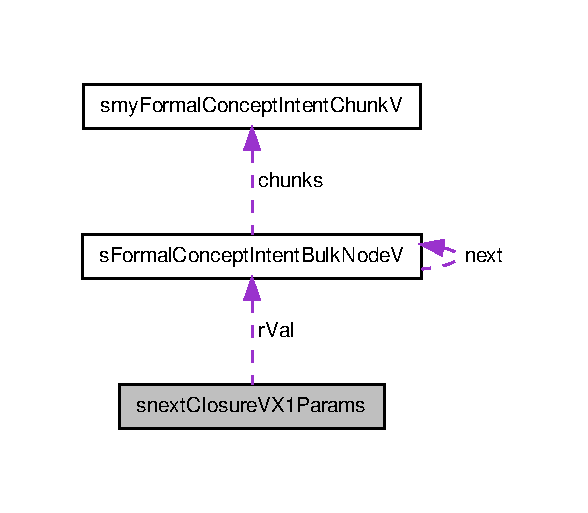
\includegraphics[width=282pt]{structsnextClosureVX1Params__coll__graph}
\end{center}
\end{figure}
\subsection*{\-Data \-Fields}
\begin{DoxyCompactItemize}
\item 
\hyperlink{fca__structs_8h_a6306c91d1e7b5237618bab6172a784a1}{\-Formal\-Concept\-Intent\-Bulk\-List\-V} \hyperlink{structsnextClosureVX1Params_a6cdec21a24ddae482ae521f8c560703a}{r\-Val}
\item 
\hyperlink{fca_8h_a98aafc7ce3efff805e9add08680b731f}{\-Formal\-Context\-V} \hyperlink{structsnextClosureVX1Params_af00ec23c26d8b4e217d29e5b949f285d}{ctx}
\item 
\hyperlink{fca_8h_aae617489ac88fff15979050721fe581f}{\-Incidence\-Vector} \hyperlink{structsnextClosureVX1Params_a61ba68899ccb6dff43b95531868f5093}{start}
\item 
\hyperlink{fca_8h_aae617489ac88fff15979050721fe581f}{\-Incidence\-Vector} \hyperlink{structsnextClosureVX1Params_a4ebb2a834d87fa4bed2bb7597ac29d23}{stop}
\end{DoxyCompactItemize}


\subsection{\-Detailed \-Description}


\-Definition at line 177 of file fca\-Vnext\-Closure\-X.\-c.



\subsection{\-Field \-Documentation}
\hypertarget{structsnextClosureVX1Params_af00ec23c26d8b4e217d29e5b949f285d}{\index{snext\-Closure\-V\-X1\-Params@{snext\-Closure\-V\-X1\-Params}!ctx@{ctx}}
\index{ctx@{ctx}!snextClosureVX1Params@{snext\-Closure\-V\-X1\-Params}}
\subsubsection[{ctx}]{\setlength{\rightskip}{0pt plus 5cm}{\bf \-Formal\-Context\-V} {\bf snext\-Closure\-V\-X1\-Params\-::ctx}}}\label{structsnextClosureVX1Params_af00ec23c26d8b4e217d29e5b949f285d}


\-Definition at line 180 of file fca\-Vnext\-Closure\-X.\-c.



\-Referenced by call\-Next\-Closure\-V\-X1(), and next\-Closure\-V\-X().

\hypertarget{structsnextClosureVX1Params_a6cdec21a24ddae482ae521f8c560703a}{\index{snext\-Closure\-V\-X1\-Params@{snext\-Closure\-V\-X1\-Params}!r\-Val@{r\-Val}}
\index{r\-Val@{r\-Val}!snextClosureVX1Params@{snext\-Closure\-V\-X1\-Params}}
\subsubsection[{r\-Val}]{\setlength{\rightskip}{0pt plus 5cm}{\bf \-Formal\-Concept\-Intent\-Bulk\-List\-V} {\bf snext\-Closure\-V\-X1\-Params\-::r\-Val}}}\label{structsnextClosureVX1Params_a6cdec21a24ddae482ae521f8c560703a}


\-Definition at line 179 of file fca\-Vnext\-Closure\-X.\-c.



\-Referenced by call\-Next\-Closure\-V\-X1(), and next\-Closure\-V\-X().

\hypertarget{structsnextClosureVX1Params_a61ba68899ccb6dff43b95531868f5093}{\index{snext\-Closure\-V\-X1\-Params@{snext\-Closure\-V\-X1\-Params}!start@{start}}
\index{start@{start}!snextClosureVX1Params@{snext\-Closure\-V\-X1\-Params}}
\subsubsection[{start}]{\setlength{\rightskip}{0pt plus 5cm}{\bf \-Incidence\-Vector} {\bf snext\-Closure\-V\-X1\-Params\-::start}}}\label{structsnextClosureVX1Params_a61ba68899ccb6dff43b95531868f5093}


\-Definition at line 181 of file fca\-Vnext\-Closure\-X.\-c.



\-Referenced by call\-Next\-Closure\-V\-X1(), and next\-Closure\-V\-X().

\hypertarget{structsnextClosureVX1Params_a4ebb2a834d87fa4bed2bb7597ac29d23}{\index{snext\-Closure\-V\-X1\-Params@{snext\-Closure\-V\-X1\-Params}!stop@{stop}}
\index{stop@{stop}!snextClosureVX1Params@{snext\-Closure\-V\-X1\-Params}}
\subsubsection[{stop}]{\setlength{\rightskip}{0pt plus 5cm}{\bf \-Incidence\-Vector} {\bf snext\-Closure\-V\-X1\-Params\-::stop}}}\label{structsnextClosureVX1Params_a4ebb2a834d87fa4bed2bb7597ac29d23}


\-Definition at line 182 of file fca\-Vnext\-Closure\-X.\-c.



\-Referenced by call\-Next\-Closure\-V\-X1(), and next\-Closure\-V\-X().



\-The documentation for this struct was generated from the following file\-:\begin{DoxyCompactItemize}
\item 
src/\hyperlink{fcaVnextClosureX_8c}{fca\-Vnext\-Closure\-X.\-c}\end{DoxyCompactItemize}

\chapter{\-File \-Documentation}
\hypertarget{cfca_8c}{\section{src/cfca.c \-File \-Reference}
\label{cfca_8c}\index{src/cfca.\-c@{src/cfca.\-c}}
}
{\ttfamily \#include $<$stdio.\-h$>$}\*
{\ttfamily \#include $<$stdlib.\-h$>$}\*
{\ttfamily \#include $<$time.\-h$>$}\*
{\ttfamily \#include \char`\"{}fca/fca.\-h\char`\"{}}\*
{\ttfamily \#include \char`\"{}fca/easy/private.\-h\char`\"{}}\*
{\ttfamily \#include \char`\"{}fca/vector/private.\-h\char`\"{}}\*
\-Include dependency graph for cfca.\-c\-:\nopagebreak
\begin{figure}[H]
\begin{center}
\leavevmode
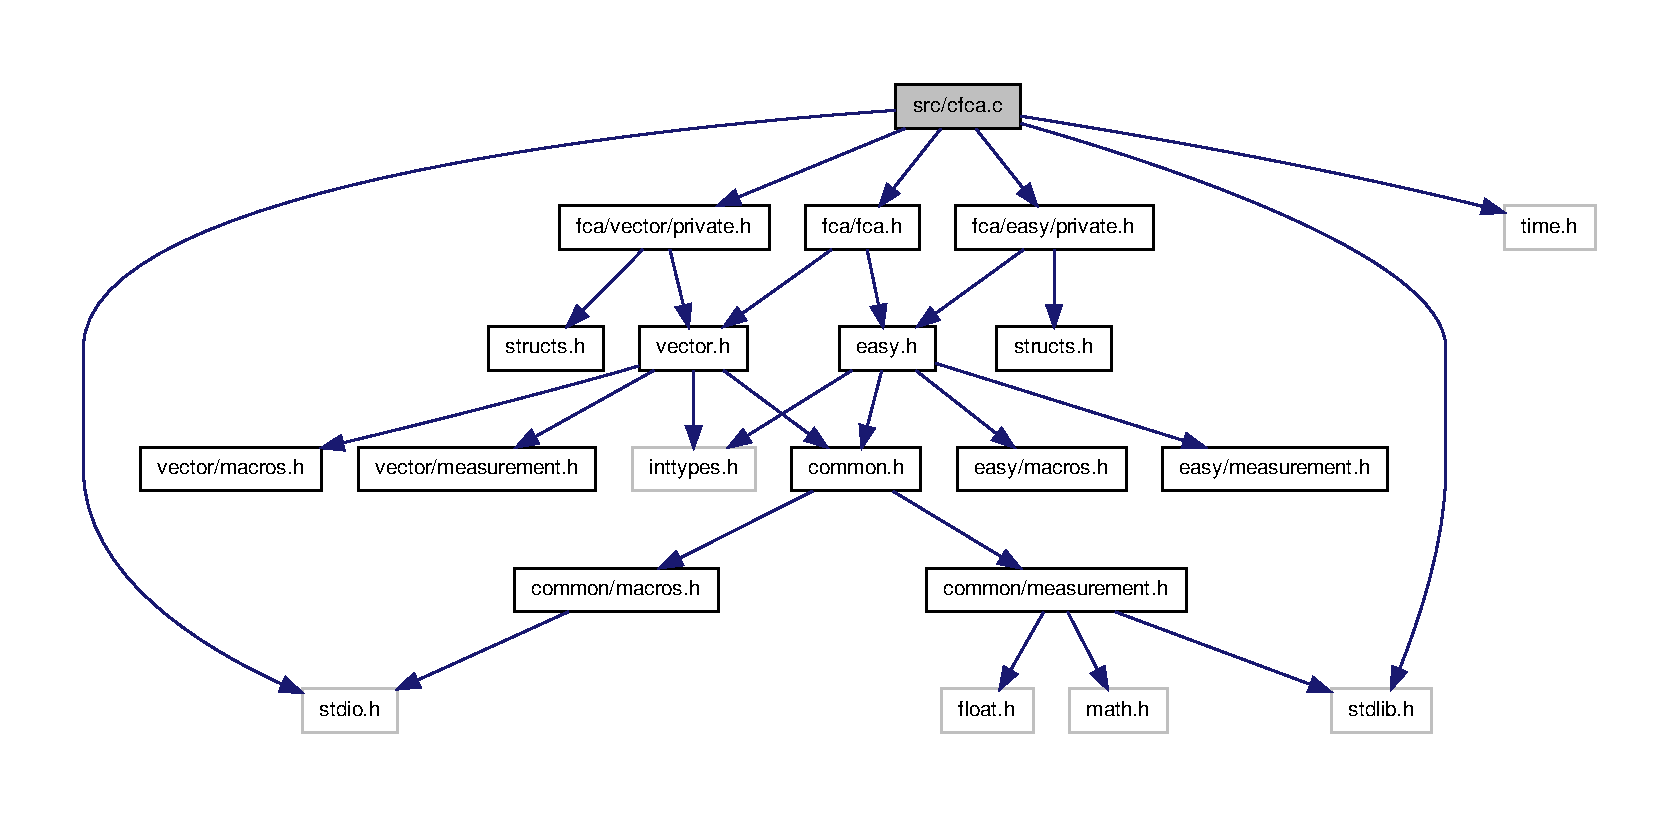
\includegraphics[width=350pt]{cfca_8c__incl}
\end{center}
\end{figure}
\subsection*{\-Functions}
\begin{DoxyCompactItemize}
\item 
int \hyperlink{cfca_8c_a840291bc02cba5474a4cb46a9b9566fe}{main} (void)
\begin{DoxyCompactList}\small\item\em \hyperlink{cfca_8c}{cfca.\-c}, (c) 2013, \-Immanuel \-Albrecht; \-Dresden \-University of \-Technology, \-Professur für die \-Psychologie des \-Lernen und \-Lehrens \end{DoxyCompactList}\end{DoxyCompactItemize}


\subsection{\-Function \-Documentation}
\hypertarget{cfca_8c_a840291bc02cba5474a4cb46a9b9566fe}{\index{cfca.\-c@{cfca.\-c}!main@{main}}
\index{main@{main}!cfca.c@{cfca.\-c}}
\subsubsection[{main}]{\setlength{\rightskip}{0pt plus 5cm}int {\bf main} (
\begin{DoxyParamCaption}
\item[{void}]{}
\end{DoxyParamCaption}
)}}\label{cfca_8c_a840291bc02cba5474a4cb46a9b9566fe}


\hyperlink{cfca_8c}{cfca.\-c}, (c) 2013, \-Immanuel \-Albrecht; \-Dresden \-University of \-Technology, \-Professur für die \-Psychologie des \-Lernen und \-Lehrens 

\-This program is free software\-: you can redistribute it and/or modify it under the terms of the \-G\-N\-U \-General \-Public \-License as published by the \-Free \-Software \-Foundation, either version 3 of the \-License, or (at your option) any later version.

\-This program is distributed in the hope that it will be useful, but \-W\-I\-T\-H\-O\-U\-T \-A\-N\-Y \-W\-A\-R\-R\-A\-N\-T\-Y; without even the implied warranty of \-M\-E\-R\-C\-H\-A\-N\-T\-A\-B\-I\-L\-I\-T\-Y or \-F\-I\-T\-N\-E\-S\-S \-F\-O\-R \-A \-P\-A\-R\-T\-I\-C\-U\-L\-A\-R \-P\-U\-R\-P\-O\-S\-E. \-See the \-G\-N\-U \-General \-Public \-License for more details.

\-You should have received a copy of the \-G\-N\-U \-General \-Public \-License along with this program. \-If not, see $<$\href{http://www.gnu.org/licenses/}{\tt http\-://www.\-gnu.\-org/licenses/}$>$. this is the main testing routine for purposes of testing the formal concept analysis implementation for errors

\begin{DoxyReturn}{\-Returns}

\end{DoxyReturn}
initialize pseudo random number generator

start tests

\-Definition at line 34 of file cfca.\-c.



\-References s\-Eta\-Function\-::\-C, calculate\-Logs(), s\-Eta\-Function\-::constants, delete\-Eta\-Function(), delete\-Formal\-Context, delete\-Log\-Cache(), new\-Condition\-Map(), new\-Fake\-Measurement(), new\-Formal\-Context\-From\-Random, new\-Log\-Cache(), new\-Uniform\-Eta\-Function(), and write\-Formal\-Context.


\begin{DoxyCode}
{
    puts("Go!");
#pragma GCC diagnostic push
#pragma GCC diagnostic ignored "-Wconversion"

    srandom(time(0));

#pragma GCC diagnostic pop

    FormalContext ctx;
    ctx = newFormalContextFromRandom(15, 30, 0.3f);

    writeFormalContext(ctx, "/home/immo/tmp/test.cxt");

    EtaFunction eta;
    eta = newUniformEtaFunction(2, 30);
    eta->C[0] = 0.05; //Type I error
    eta->C[1] = 0.10; //Type II error

    LogCache logC;
    logC = newLogCache(eta->constants);
    calculateLogs(eta,logC);


    FormalContext B;
    B = newFakeMeasurement(ctx,eta,150);
    writeFormalContext(B, "/home/immo/tmp/test_B.cxt");

    ConditionMap c;
    c = newConditionMap(150);


    deleteLogCache(&logC);
    deleteEtaFunction(&eta);
    deleteFormalContext(&B);
    deleteFormalContext(&ctx);

    puts("done.");
    return EXIT_SUCCESS;
}
\end{DoxyCode}


\-Here is the call graph for this function\-:\nopagebreak
\begin{figure}[H]
\begin{center}
\leavevmode
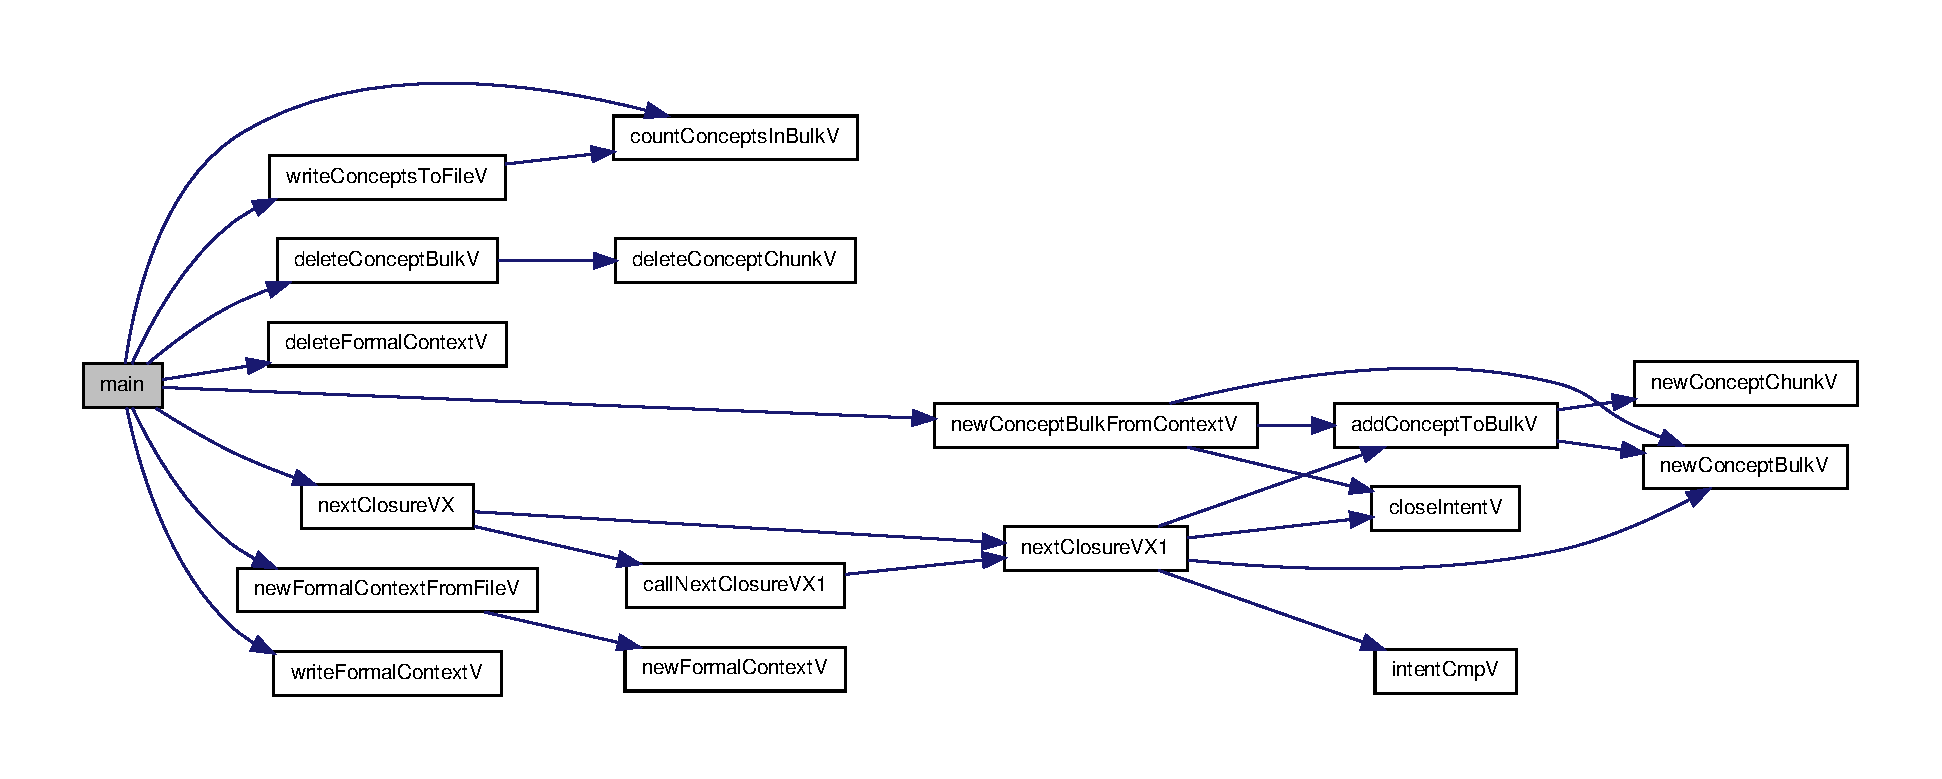
\includegraphics[width=350pt]{cfca_8c_a840291bc02cba5474a4cb46a9b9566fe_cgraph}
\end{center}
\end{figure}



\hypertarget{common_8h}{\section{src/fca/common.h \-File \-Reference}
\label{common_8h}\index{src/fca/common.\-h@{src/fca/common.\-h}}
}
{\ttfamily \#include \char`\"{}common/macros.\-h\char`\"{}}\*
{\ttfamily \#include \char`\"{}common/measurement.\-h\char`\"{}}\*
\-Include dependency graph for common.\-h\-:
\nopagebreak
\begin{figure}[H]
\begin{center}
\leavevmode
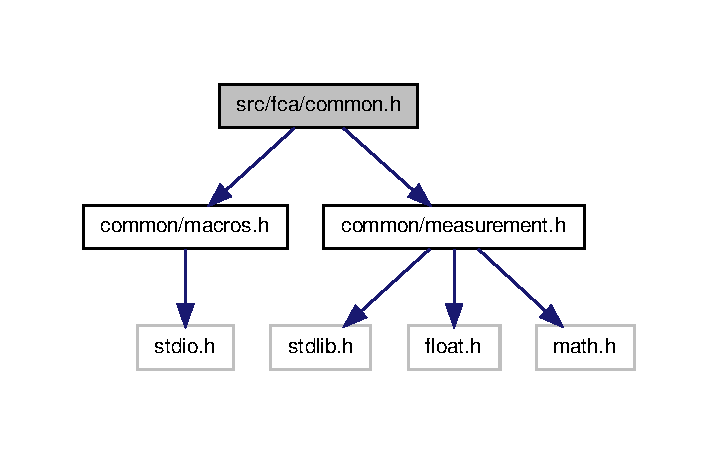
\includegraphics[width=320pt]{common_8h__incl}
\end{center}
\end{figure}
\-This graph shows which files directly or indirectly include this file\-:
\nopagebreak
\begin{figure}[H]
\begin{center}
\leavevmode
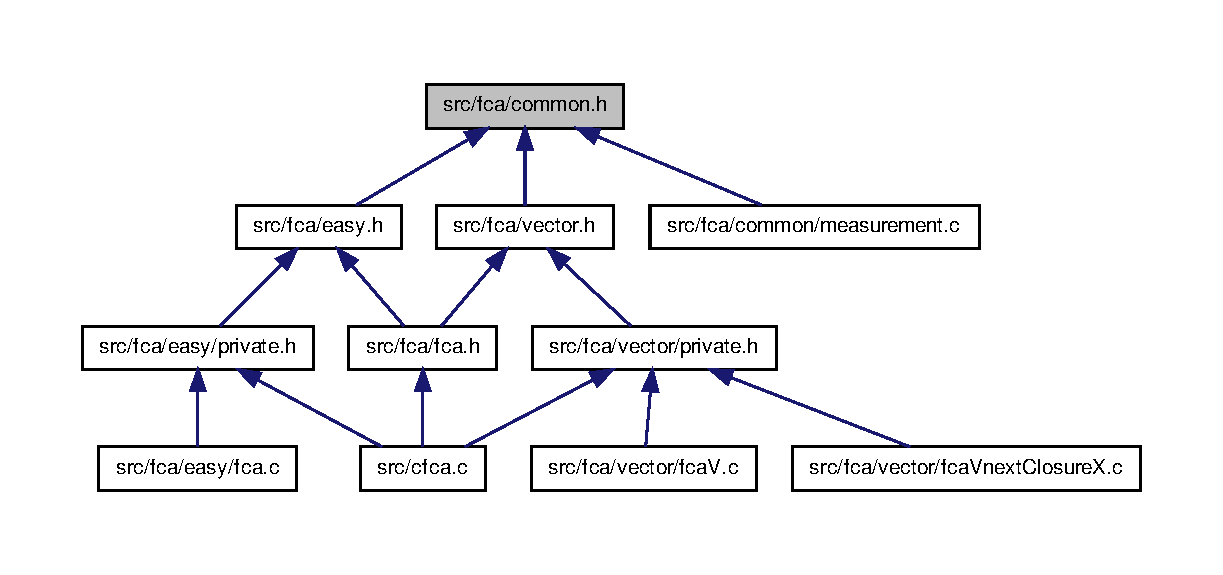
\includegraphics[width=350pt]{common_8h__dep__incl}
\end{center}
\end{figure}

\hypertarget{common_2macros_8h}{\section{src/fca/common/macros.h \-File \-Reference}
\label{common_2macros_8h}\index{src/fca/common/macros.\-h@{src/fca/common/macros.\-h}}
}
{\ttfamily \#include $<$stdio.\-h$>$}\*
\-Include dependency graph for macros.\-h\-:\nopagebreak
\begin{figure}[H]
\begin{center}
\leavevmode
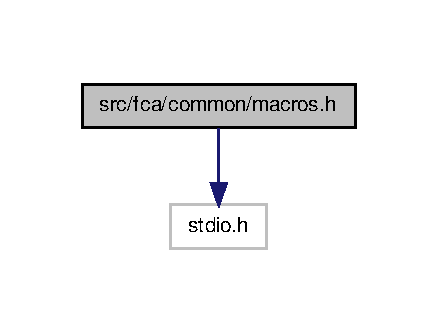
\includegraphics[width=210pt]{common_2macros_8h__incl}
\end{center}
\end{figure}
\-This graph shows which files directly or indirectly include this file\-:\nopagebreak
\begin{figure}[H]
\begin{center}
\leavevmode
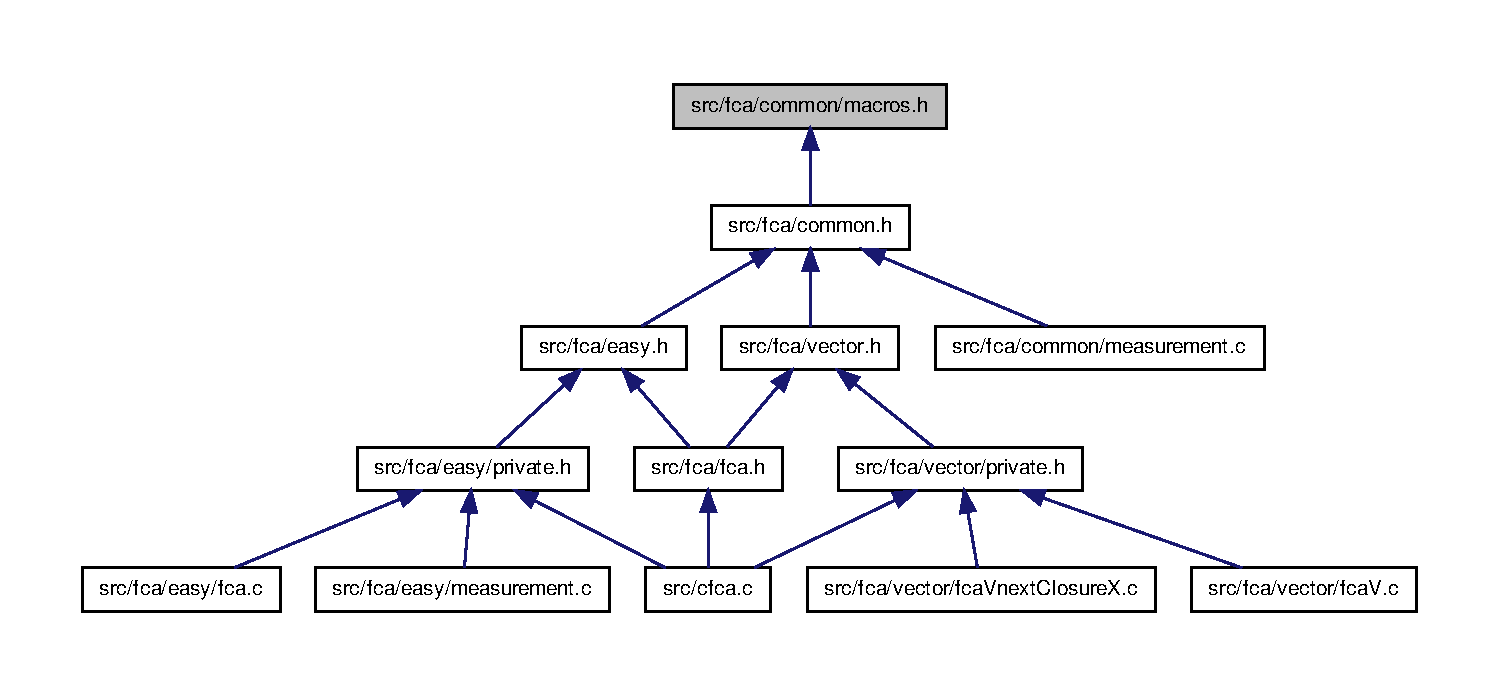
\includegraphics[width=350pt]{common_2macros_8h__dep__incl}
\end{center}
\end{figure}
\subsection*{\-Defines}
\begin{DoxyCompactItemize}
\item 
\#define \hyperlink{common_2macros_8h_a740a16a7eb505fa8d595a191feed0941}{\-R\-E\-T\-U\-R\-N\-\_\-\-I\-F\-\_\-\-Z\-E\-R\-O}(x)~\{if (((x) == (void$\ast$)0)) \{fprintf(stderr, \char`\"{}\-W\-A\-R\-N\-I\-N\-G\-: \-Z\-E\-R\-O pointer \%s in \%s \mbox{[}\%s\-:\%u\mbox{]}$\backslash$n\char`\"{}, \#x, \-\_\-\-\_\-\-F\-U\-N\-C\-T\-I\-O\-N\-\_\-\-\_\-, \-\_\-\-\_\-\-F\-I\-L\-E\-\_\-\-\_\-,\-\_\-\-\_\-\-L\-I\-N\-E\-\_\-\-\_\-); return;\}\}
\begin{DoxyCompactList}\small\item\em fca\-\_\-macros.\-h, (c) 2013, \-Immanuel \-Albrecht; \-Dresden \-University of \-Technology, \-Professur für die \-Psychologie des \-Lernen und \-Lehrens \end{DoxyCompactList}\item 
\#define \hyperlink{common_2macros_8h_aecdd5bdf585ad172473c37e40bfac5ff}{\-R\-E\-T\-U\-R\-N\-\_\-\-Z\-E\-R\-O\-\_\-\-I\-F\-\_\-\-Z\-E\-R\-O}(x)~\{if (((x) == (void$\ast$)0)) \{fprintf(stderr, \char`\"{}\-W\-A\-R\-N\-I\-N\-G\-: \-Z\-E\-R\-O pointer \%s in \%s \mbox{[}\%s\-:\%u\mbox{]}$\backslash$n\char`\"{}, \#x, \-\_\-\-\_\-\-F\-U\-N\-C\-T\-I\-O\-N\-\_\-\-\_\-, \-\_\-\-\_\-\-F\-I\-L\-E\-\_\-\-\_\-,\-\_\-\-\_\-\-L\-I\-N\-E\-\_\-\-\_\-); return 0;\}\}
\begin{DoxyCompactList}\small\item\em checks whether x == (void$\ast$)0, and returns 0; \end{DoxyCompactList}\item 
\#define \hyperlink{common_2macros_8h_a204342bc46513e130770caef51b50d55}{\-R\-E\-T\-U\-R\-N\-\_\-\-Z\-E\-R\-O\-\_\-\-I\-F\-\_\-\-Z\-E\-R\-O\-I}(x)~\{if (((x) == 0)) \{fprintf(stderr, \char`\"{}\-W\-A\-R\-N\-I\-N\-G\-: \-Z\-E\-R\-O \%s in \%s \mbox{[}\%s\-:\%u\mbox{]}$\backslash$n\char`\"{}, \#x, \-\_\-\-\_\-\-F\-U\-N\-C\-T\-I\-O\-N\-\_\-\-\_\-, \-\_\-\-\_\-\-F\-I\-L\-E\-\_\-\-\_\-,\-\_\-\-\_\-\-L\-I\-N\-E\-\_\-\-\_\-); return 0;\}\}
\begin{DoxyCompactList}\small\item\em checks whether x == 0, and returns 0; \end{DoxyCompactList}\item 
\#define \hyperlink{common_2macros_8h_a8d200ab641cd359687ca7bbd465b219a}{\-W\-A\-R\-N\-\_\-\-I\-F\-\_\-\-U\-N\-E\-Q\-U\-A\-L\-\_\-\-D\-O}(x, y, d)~\{if (((x) != (y))) \{fprintf(stderr, \char`\"{}\-W\-A\-R\-N\-I\-N\-G\-: \%s \-N\-O\-T \-E\-Q\-U\-A\-L \-T\-O \%s in \%s \mbox{[}\%s\-:\%u\mbox{]}$\backslash$n\char`\"{}, \#x, \#y, \-\_\-\-\_\-\-F\-U\-N\-C\-T\-I\-O\-N\-\_\-\-\_\-, \-\_\-\-\_\-\-F\-I\-L\-E\-\_\-\-\_\-,\-\_\-\-\_\-\-L\-I\-N\-E\-\_\-\-\_\-); d;\}\}
\begin{DoxyCompactList}\small\item\em if x!=y, prints a warning and calls the statement d \end{DoxyCompactList}\item 
\#define \hyperlink{common_2macros_8h_aad9d5baa0093f289563ebcebc5a84de9}{\-W\-A\-R\-N\-\_\-\-I\-F\-\_\-\-G\-E\-Q\-\_\-\-D\-O}(x, y, d)~\{if (((x) $>$= (y))) \{fprintf(stderr, \char`\"{}\-W\-A\-R\-N\-I\-N\-G\-: \%s \-N\-O\-T \-E\-Q\-U\-A\-L \-T\-O \%s in \%s \mbox{[}\%s\-:\%u\mbox{]}$\backslash$n\char`\"{}, \#x, \#y, \-\_\-\-\_\-\-F\-U\-N\-C\-T\-I\-O\-N\-\_\-\-\_\-, \-\_\-\-\_\-\-F\-I\-L\-E\-\_\-\-\_\-,\-\_\-\-\_\-\-L\-I\-N\-E\-\_\-\-\_\-); d;\}\}
\begin{DoxyCompactList}\small\item\em if x$>$=y, prints a warning and calls the statement d \end{DoxyCompactList}\item 
\#define \hyperlink{common_2macros_8h_a3acffbd305ee72dcd4593c0d8af64a4f}{\-M\-I\-N}(a, b)~(((a)$<$(b))?(a)\-:(b))
\begin{DoxyCompactList}\small\item\em gives minimum \end{DoxyCompactList}\item 
\#define \hyperlink{common_2macros_8h_afa99ec4acc4ecb2dc3c2d05da15d0e3f}{\-M\-A\-X}(a, b)~(((a)$>$(b))?(a)\-:(b))
\begin{DoxyCompactList}\small\item\em gives maximum \end{DoxyCompactList}\end{DoxyCompactItemize}


\subsection{\-Define \-Documentation}
\hypertarget{common_2macros_8h_afa99ec4acc4ecb2dc3c2d05da15d0e3f}{\index{common/macros.\-h@{common/macros.\-h}!\-M\-A\-X@{\-M\-A\-X}}
\index{\-M\-A\-X@{\-M\-A\-X}!common/macros.h@{common/macros.\-h}}
\subsubsection[{\-M\-A\-X}]{\setlength{\rightskip}{0pt plus 5cm}\#define {\bf \-M\-A\-X}(
\begin{DoxyParamCaption}
\item[{}]{a, }
\item[{}]{b}
\end{DoxyParamCaption}
)~(((a)$>$(b))?(a)\-:(b))}}\label{common_2macros_8h_afa99ec4acc4ecb2dc3c2d05da15d0e3f}


gives maximum 



\-Definition at line 71 of file macros.\-h.

\hypertarget{common_2macros_8h_a3acffbd305ee72dcd4593c0d8af64a4f}{\index{common/macros.\-h@{common/macros.\-h}!\-M\-I\-N@{\-M\-I\-N}}
\index{\-M\-I\-N@{\-M\-I\-N}!common/macros.h@{common/macros.\-h}}
\subsubsection[{\-M\-I\-N}]{\setlength{\rightskip}{0pt plus 5cm}\#define {\bf \-M\-I\-N}(
\begin{DoxyParamCaption}
\item[{}]{a, }
\item[{}]{b}
\end{DoxyParamCaption}
)~(((a)$<$(b))?(a)\-:(b))}}\label{common_2macros_8h_a3acffbd305ee72dcd4593c0d8af64a4f}


gives minimum 



\-Definition at line 64 of file macros.\-h.



\-Referenced by new\-Fake\-Measurement(), new\-Formal\-Context\-From\-File(), and new\-Formal\-Context\-From\-File\-V().

\hypertarget{common_2macros_8h_a740a16a7eb505fa8d595a191feed0941}{\index{common/macros.\-h@{common/macros.\-h}!\-R\-E\-T\-U\-R\-N\-\_\-\-I\-F\-\_\-\-Z\-E\-R\-O@{\-R\-E\-T\-U\-R\-N\-\_\-\-I\-F\-\_\-\-Z\-E\-R\-O}}
\index{\-R\-E\-T\-U\-R\-N\-\_\-\-I\-F\-\_\-\-Z\-E\-R\-O@{\-R\-E\-T\-U\-R\-N\-\_\-\-I\-F\-\_\-\-Z\-E\-R\-O}!common/macros.h@{common/macros.\-h}}
\subsubsection[{\-R\-E\-T\-U\-R\-N\-\_\-\-I\-F\-\_\-\-Z\-E\-R\-O}]{\setlength{\rightskip}{0pt plus 5cm}\#define {\bf \-R\-E\-T\-U\-R\-N\-\_\-\-I\-F\-\_\-\-Z\-E\-R\-O}(
\begin{DoxyParamCaption}
\item[{}]{x}
\end{DoxyParamCaption}
)~\{if (((x) == (void$\ast$)0)) \{fprintf(stderr, \char`\"{}\-W\-A\-R\-N\-I\-N\-G\-: \-Z\-E\-R\-O pointer \%s in \%s \mbox{[}\%s\-:\%u\mbox{]}$\backslash$n\char`\"{}, \#x, \-\_\-\-\_\-\-F\-U\-N\-C\-T\-I\-O\-N\-\_\-\-\_\-, \-\_\-\-\_\-\-F\-I\-L\-E\-\_\-\-\_\-,\-\_\-\-\_\-\-L\-I\-N\-E\-\_\-\-\_\-); return;\}\}}}\label{common_2macros_8h_a740a16a7eb505fa8d595a191feed0941}


fca\-\_\-macros.\-h, (c) 2013, \-Immanuel \-Albrecht; \-Dresden \-University of \-Technology, \-Professur für die \-Psychologie des \-Lernen und \-Lehrens 

\-This program is free software\-: you can redistribute it and/or modify it under the terms of the \-G\-N\-U \-General \-Public \-License as published by the \-Free \-Software \-Foundation, either version 3 of the \-License, or (at your option) any later version.

\-This program is distributed in the hope that it will be useful, but \-W\-I\-T\-H\-O\-U\-T \-A\-N\-Y \-W\-A\-R\-R\-A\-N\-T\-Y; without even the implied warranty of \-M\-E\-R\-C\-H\-A\-N\-T\-A\-B\-I\-L\-I\-T\-Y or \-F\-I\-T\-N\-E\-S\-S \-F\-O\-R \-A \-P\-A\-R\-T\-I\-C\-U\-L\-A\-R \-P\-U\-R\-P\-O\-S\-E. \-See the \-G\-N\-U \-General \-Public \-License for more details.

\-You should have received a copy of the \-G\-N\-U \-General \-Public \-License along with this program. \-If not, see $<$\href{http://www.gnu.org/licenses/}{\tt http\-://www.\-gnu.\-org/licenses/}$>$.

checks whether x == 0, and returns 

\-Definition at line 29 of file macros.\-h.



\-Referenced by calculate\-Likelihood(), delete\-Commutative\-Product(), delete\-Concept\-Bulk(), delete\-Concept\-Bulk\-V(), delete\-Concept\-Chunk(), delete\-Concept\-Chunk\-V(), delete\-Condition\-Map(), delete\-Distance\-Matrix(), delete\-Eta\-Function(), delete\-Formal\-Context(), delete\-Formal\-Context\-V(), delete\-Log\-Cache(), optimize\-Approximation\-Context(), optimize\-Condition\-Map(), write\-Concepts\-To\-File(), write\-Concepts\-To\-File\-V(), write\-Distances\-To\-File(), write\-Formal\-Context(), and write\-Formal\-Context\-V().

\hypertarget{common_2macros_8h_aecdd5bdf585ad172473c37e40bfac5ff}{\index{common/macros.\-h@{common/macros.\-h}!\-R\-E\-T\-U\-R\-N\-\_\-\-Z\-E\-R\-O\-\_\-\-I\-F\-\_\-\-Z\-E\-R\-O@{\-R\-E\-T\-U\-R\-N\-\_\-\-Z\-E\-R\-O\-\_\-\-I\-F\-\_\-\-Z\-E\-R\-O}}
\index{\-R\-E\-T\-U\-R\-N\-\_\-\-Z\-E\-R\-O\-\_\-\-I\-F\-\_\-\-Z\-E\-R\-O@{\-R\-E\-T\-U\-R\-N\-\_\-\-Z\-E\-R\-O\-\_\-\-I\-F\-\_\-\-Z\-E\-R\-O}!common/macros.h@{common/macros.\-h}}
\subsubsection[{\-R\-E\-T\-U\-R\-N\-\_\-\-Z\-E\-R\-O\-\_\-\-I\-F\-\_\-\-Z\-E\-R\-O}]{\setlength{\rightskip}{0pt plus 5cm}\#define {\bf \-R\-E\-T\-U\-R\-N\-\_\-\-Z\-E\-R\-O\-\_\-\-I\-F\-\_\-\-Z\-E\-R\-O}(
\begin{DoxyParamCaption}
\item[{}]{x}
\end{DoxyParamCaption}
)~\{if (((x) == (void$\ast$)0)) \{fprintf(stderr, \char`\"{}\-W\-A\-R\-N\-I\-N\-G\-: \-Z\-E\-R\-O pointer \%s in \%s \mbox{[}\%s\-:\%u\mbox{]}$\backslash$n\char`\"{}, \#x, \-\_\-\-\_\-\-F\-U\-N\-C\-T\-I\-O\-N\-\_\-\-\_\-, \-\_\-\-\_\-\-F\-I\-L\-E\-\_\-\-\_\-,\-\_\-\-\_\-\-L\-I\-N\-E\-\_\-\-\_\-); return 0;\}\}}}\label{common_2macros_8h_aecdd5bdf585ad172473c37e40bfac5ff}


checks whether x == (void$\ast$)0, and returns 0; 



\-Definition at line 36 of file macros.\-h.



\-Referenced by add\-Concept\-To\-Bulk(), add\-Concept\-To\-Bulk\-V(), count\-Concepts\-In\-Bulk(), count\-Concepts\-In\-Bulk\-V(), count\-Context\-Concepts(), count\-Context\-Concepts2(), count\-Context\-Concepts\-V(), log\-Probability\-From\-Product(), new\-Concept\-Bulk\-From\-Context(), new\-Concept\-Bulk\-From\-Context\-V(), new\-Distance\-Matrix\-From\-Context(), new\-Fake\-Measurement(), new\-Formal\-Context\-From\-File(), new\-Formal\-Context\-From\-File\-V(), next\-Closure\-V\-X(), and next\-Closure\-V\-X1().

\hypertarget{common_2macros_8h_a204342bc46513e130770caef51b50d55}{\index{common/macros.\-h@{common/macros.\-h}!\-R\-E\-T\-U\-R\-N\-\_\-\-Z\-E\-R\-O\-\_\-\-I\-F\-\_\-\-Z\-E\-R\-O\-I@{\-R\-E\-T\-U\-R\-N\-\_\-\-Z\-E\-R\-O\-\_\-\-I\-F\-\_\-\-Z\-E\-R\-O\-I}}
\index{\-R\-E\-T\-U\-R\-N\-\_\-\-Z\-E\-R\-O\-\_\-\-I\-F\-\_\-\-Z\-E\-R\-O\-I@{\-R\-E\-T\-U\-R\-N\-\_\-\-Z\-E\-R\-O\-\_\-\-I\-F\-\_\-\-Z\-E\-R\-O\-I}!common/macros.h@{common/macros.\-h}}
\subsubsection[{\-R\-E\-T\-U\-R\-N\-\_\-\-Z\-E\-R\-O\-\_\-\-I\-F\-\_\-\-Z\-E\-R\-O\-I}]{\setlength{\rightskip}{0pt plus 5cm}\#define {\bf \-R\-E\-T\-U\-R\-N\-\_\-\-Z\-E\-R\-O\-\_\-\-I\-F\-\_\-\-Z\-E\-R\-O\-I}(
\begin{DoxyParamCaption}
\item[{}]{x}
\end{DoxyParamCaption}
)~\{if (((x) == 0)) \{fprintf(stderr, \char`\"{}\-W\-A\-R\-N\-I\-N\-G\-: \-Z\-E\-R\-O \%s in \%s \mbox{[}\%s\-:\%u\mbox{]}$\backslash$n\char`\"{}, \#x, \-\_\-\-\_\-\-F\-U\-N\-C\-T\-I\-O\-N\-\_\-\-\_\-, \-\_\-\-\_\-\-F\-I\-L\-E\-\_\-\-\_\-,\-\_\-\-\_\-\-L\-I\-N\-E\-\_\-\-\_\-); return 0;\}\}}}\label{common_2macros_8h_a204342bc46513e130770caef51b50d55}


checks whether x == 0, and returns 0; 



\-Definition at line 42 of file macros.\-h.



\-Referenced by new\-Commutative\-Product(), new\-Condition\-Map(), new\-Distance\-Matrix(), and new\-Eta\-Function().

\hypertarget{common_2macros_8h_aad9d5baa0093f289563ebcebc5a84de9}{\index{common/macros.\-h@{common/macros.\-h}!\-W\-A\-R\-N\-\_\-\-I\-F\-\_\-\-G\-E\-Q\-\_\-\-D\-O@{\-W\-A\-R\-N\-\_\-\-I\-F\-\_\-\-G\-E\-Q\-\_\-\-D\-O}}
\index{\-W\-A\-R\-N\-\_\-\-I\-F\-\_\-\-G\-E\-Q\-\_\-\-D\-O@{\-W\-A\-R\-N\-\_\-\-I\-F\-\_\-\-G\-E\-Q\-\_\-\-D\-O}!common/macros.h@{common/macros.\-h}}
\subsubsection[{\-W\-A\-R\-N\-\_\-\-I\-F\-\_\-\-G\-E\-Q\-\_\-\-D\-O}]{\setlength{\rightskip}{0pt plus 5cm}\#define {\bf \-W\-A\-R\-N\-\_\-\-I\-F\-\_\-\-G\-E\-Q\-\_\-\-D\-O}(
\begin{DoxyParamCaption}
\item[{}]{x, }
\item[{}]{y, }
\item[{}]{d}
\end{DoxyParamCaption}
)~\{if (((x) $>$= (y))) \{fprintf(stderr, \char`\"{}\-W\-A\-R\-N\-I\-N\-G\-: \%s \-N\-O\-T \-E\-Q\-U\-A\-L \-T\-O \%s in \%s \mbox{[}\%s\-:\%u\mbox{]}$\backslash$n\char`\"{}, \#x, \#y, \-\_\-\-\_\-\-F\-U\-N\-C\-T\-I\-O\-N\-\_\-\-\_\-, \-\_\-\-\_\-\-F\-I\-L\-E\-\_\-\-\_\-,\-\_\-\-\_\-\-L\-I\-N\-E\-\_\-\-\_\-); d;\}\}}}\label{common_2macros_8h_aad9d5baa0093f289563ebcebc5a84de9}


if x$>$=y, prints a warning and calls the statement d 



\-Definition at line 56 of file macros.\-h.



\-Referenced by calculate\-Likelihood().

\hypertarget{common_2macros_8h_a8d200ab641cd359687ca7bbd465b219a}{\index{common/macros.\-h@{common/macros.\-h}!\-W\-A\-R\-N\-\_\-\-I\-F\-\_\-\-U\-N\-E\-Q\-U\-A\-L\-\_\-\-D\-O@{\-W\-A\-R\-N\-\_\-\-I\-F\-\_\-\-U\-N\-E\-Q\-U\-A\-L\-\_\-\-D\-O}}
\index{\-W\-A\-R\-N\-\_\-\-I\-F\-\_\-\-U\-N\-E\-Q\-U\-A\-L\-\_\-\-D\-O@{\-W\-A\-R\-N\-\_\-\-I\-F\-\_\-\-U\-N\-E\-Q\-U\-A\-L\-\_\-\-D\-O}!common/macros.h@{common/macros.\-h}}
\subsubsection[{\-W\-A\-R\-N\-\_\-\-I\-F\-\_\-\-U\-N\-E\-Q\-U\-A\-L\-\_\-\-D\-O}]{\setlength{\rightskip}{0pt plus 5cm}\#define {\bf \-W\-A\-R\-N\-\_\-\-I\-F\-\_\-\-U\-N\-E\-Q\-U\-A\-L\-\_\-\-D\-O}(
\begin{DoxyParamCaption}
\item[{}]{x, }
\item[{}]{y, }
\item[{}]{d}
\end{DoxyParamCaption}
)~\{if (((x) != (y))) \{fprintf(stderr, \char`\"{}\-W\-A\-R\-N\-I\-N\-G\-: \%s \-N\-O\-T \-E\-Q\-U\-A\-L \-T\-O \%s in \%s \mbox{[}\%s\-:\%u\mbox{]}$\backslash$n\char`\"{}, \#x, \#y, \-\_\-\-\_\-\-F\-U\-N\-C\-T\-I\-O\-N\-\_\-\-\_\-, \-\_\-\-\_\-\-F\-I\-L\-E\-\_\-\-\_\-,\-\_\-\-\_\-\-L\-I\-N\-E\-\_\-\-\_\-); d;\}\}}}\label{common_2macros_8h_a8d200ab641cd359687ca7bbd465b219a}


if x!=y, prints a warning and calls the statement d 



\-Definition at line 49 of file macros.\-h.



\-Referenced by calculate\-Likelihood(), calculate\-Logs(), log\-Probability\-From\-Product(), new\-Distance\-Matrix\-From\-Context(), new\-Fake\-Measurement(), optimize\-Approximation\-Context(), optimize\-Condition\-Map(), write\-Concepts\-To\-File(), and write\-Concepts\-To\-File\-V().


\hypertarget{easy_2macros_8h}{\section{src/fca/easy/macros.h \-File \-Reference}
\label{easy_2macros_8h}\index{src/fca/easy/macros.\-h@{src/fca/easy/macros.\-h}}
}


\hyperlink{easy_2macros_8h}{easy/macros.\-h}, (c) 2013, \-Immanuel \-Albrecht; \-Dresden \-University of \-Technology, \-Professur für die \-Psychologie des \-Lernen und \-Lehrens  


\-This graph shows which files directly or indirectly include this file\-:\nopagebreak
\begin{figure}[H]
\begin{center}
\leavevmode
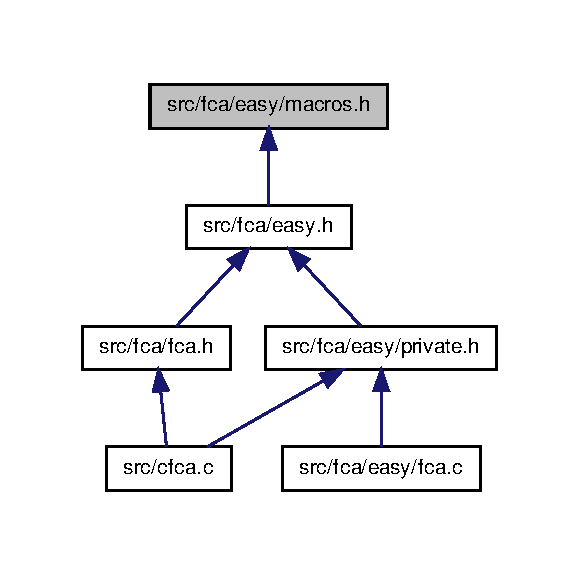
\includegraphics[width=350pt]{easy_2macros_8h__dep__incl}
\end{center}
\end{figure}
\subsection*{\-Defines}
\begin{DoxyCompactItemize}
\item 
\#define \hyperlink{easy_2macros_8h_ad4734e82cfd82a52750c823e4a3f745a}{\-I\-N\-C\-I\-D\-E\-S}(x)~(((x)\&1))
\begin{DoxyCompactList}\small\item\em checks whether something incides by testing the 1-\/bit \end{DoxyCompactList}\item 
\#define \hyperlink{easy_2macros_8h_ab0ba4dd6e237b96132c0a66be2fb3bc2}{\-C\-L\-E\-A\-R}(x)~\{ (x) = 0; \}
\begin{DoxyCompactList}\small\item\em clears the mark \end{DoxyCompactList}\item 
\#define \hyperlink{easy_2macros_8h_add682bc16cfd313b57c9dc8400158bc0}{\-C\-R\-O\-S\-S}(x)~\{ (x) = 1; \}
\begin{DoxyCompactList}\small\item\em sets the mark \end{DoxyCompactList}\item 
\#define \hyperlink{easy_2macros_8h_a6716296e0c0390116c559152e613eb17}{\-C\-E\-L\-L}(g, \-I, m)~((\-I)-\/$>$incidence\mbox{[}(\-I)-\/$>$attributes $\ast$ (g) + (m)\mbox{]})
\begin{DoxyCompactList}\small\item\em results in the cell that encodes whether g incides with m \end{DoxyCompactList}\item 
\#define \hyperlink{easy_2macros_8h_ac504a61c4c85120715ba5d25a72148b1}{g\-Im}(g, \-I, m)~\hyperlink{easy_2macros_8h_ad4734e82cfd82a52750c823e4a3f745a}{\-I\-N\-C\-I\-D\-E\-S}(\hyperlink{easy_2macros_8h_a6716296e0c0390116c559152e613eb17}{\-C\-E\-L\-L}( (g) , (\-I) , (m)))
\begin{DoxyCompactList}\small\item\em test whether g and m incides \end{DoxyCompactList}\end{DoxyCompactItemize}


\subsection{\-Detailed \-Description}
\hyperlink{easy_2macros_8h}{easy/macros.\-h}, (c) 2013, \-Immanuel \-Albrecht; \-Dresden \-University of \-Technology, \-Professur für die \-Psychologie des \-Lernen und \-Lehrens \-This program is free software\-: you can redistribute it and/or modify it under the terms of the \-G\-N\-U \-General \-Public \-License as published by the \-Free \-Software \-Foundation, either version 3 of the \-License, or (at your option) any later version.

\-This program is distributed in the hope that it will be useful, but \-W\-I\-T\-H\-O\-U\-T \-A\-N\-Y \-W\-A\-R\-R\-A\-N\-T\-Y; without even the implied warranty of \-M\-E\-R\-C\-H\-A\-N\-T\-A\-B\-I\-L\-I\-T\-Y or \-F\-I\-T\-N\-E\-S\-S \-F\-O\-R \-A \-P\-A\-R\-T\-I\-C\-U\-L\-A\-R \-P\-U\-R\-P\-O\-S\-E. \-See the \-G\-N\-U \-General \-Public \-License for more details.

\-You should have received a copy of the \-G\-N\-U \-General \-Public \-License along with this program. \-If not, see $<$\href{http://www.gnu.org/licenses/}{\tt http\-://www.\-gnu.\-org/licenses/}$>$. \-These macros are used for \-Incidence\-Cell array implementations of formal contexts. \-Such implementations are easier to debug, but take up far too much memory for big scale contexts 

\-Definition in file \hyperlink{easy_2macros_8h_source}{macros.\-h}.



\subsection{\-Define \-Documentation}
\hypertarget{easy_2macros_8h_a6716296e0c0390116c559152e613eb17}{\index{easy/macros.\-h@{easy/macros.\-h}!\-C\-E\-L\-L@{\-C\-E\-L\-L}}
\index{\-C\-E\-L\-L@{\-C\-E\-L\-L}!easy/macros.h@{easy/macros.\-h}}
\subsubsection[{\-C\-E\-L\-L}]{\setlength{\rightskip}{0pt plus 5cm}\#define {\bf \-C\-E\-L\-L}(
\begin{DoxyParamCaption}
\item[{}]{g, }
\item[{}]{\-I, }
\item[{}]{m}
\end{DoxyParamCaption}
)~((\-I)-\/$>$incidence\mbox{[}(\-I)-\/$>$attributes $\ast$ (g) + (m)\mbox{]})}}\label{easy_2macros_8h_a6716296e0c0390116c559152e613eb17}


results in the cell that encodes whether g incides with m 

\-I may be a formal context, then g refers to the object number, or \-I may be a chunk of formal concepts, then g refers to the concept number. 

\-Definition at line 61 of file macros.\-h.



\-Referenced by add\-Concept\-To\-Bulk(), new\-Fake\-Measurement(), new\-Formal\-Context\-From\-File(), and new\-Formal\-Context\-From\-Random().

\hypertarget{easy_2macros_8h_ab0ba4dd6e237b96132c0a66be2fb3bc2}{\index{easy/macros.\-h@{easy/macros.\-h}!\-C\-L\-E\-A\-R@{\-C\-L\-E\-A\-R}}
\index{\-C\-L\-E\-A\-R@{\-C\-L\-E\-A\-R}!easy/macros.h@{easy/macros.\-h}}
\subsubsection[{\-C\-L\-E\-A\-R}]{\setlength{\rightskip}{0pt plus 5cm}\#define {\bf \-C\-L\-E\-A\-R}(
\begin{DoxyParamCaption}
\item[{}]{x}
\end{DoxyParamCaption}
)~\{ (x) = 0; \}}}\label{easy_2macros_8h_ab0ba4dd6e237b96132c0a66be2fb3bc2}


clears the mark 



\-Definition at line 42 of file macros.\-h.



\-Referenced by close\-Intent(), close\-Intent2(), count\-Context\-Concepts(), count\-Context\-Concepts2(), and new\-Concept\-Bulk\-From\-Context().

\hypertarget{easy_2macros_8h_add682bc16cfd313b57c9dc8400158bc0}{\index{easy/macros.\-h@{easy/macros.\-h}!\-C\-R\-O\-S\-S@{\-C\-R\-O\-S\-S}}
\index{\-C\-R\-O\-S\-S@{\-C\-R\-O\-S\-S}!easy/macros.h@{easy/macros.\-h}}
\subsubsection[{\-C\-R\-O\-S\-S}]{\setlength{\rightskip}{0pt plus 5cm}\#define {\bf \-C\-R\-O\-S\-S}(
\begin{DoxyParamCaption}
\item[{}]{x}
\end{DoxyParamCaption}
)~\{ (x) = 1; \}}}\label{easy_2macros_8h_add682bc16cfd313b57c9dc8400158bc0}


sets the mark 



\-Definition at line 50 of file macros.\-h.



\-Referenced by close\-Intent(), close\-Intent2(), count\-Context\-Concepts(), count\-Context\-Concepts2(), new\-Concept\-Bulk\-From\-Context(), new\-Fake\-Measurement(), new\-Formal\-Context\-From\-File(), and new\-Formal\-Context\-From\-Random().

\hypertarget{easy_2macros_8h_ac504a61c4c85120715ba5d25a72148b1}{\index{easy/macros.\-h@{easy/macros.\-h}!g\-Im@{g\-Im}}
\index{g\-Im@{g\-Im}!easy/macros.h@{easy/macros.\-h}}
\subsubsection[{g\-Im}]{\setlength{\rightskip}{0pt plus 5cm}\#define {\bf g\-Im}(
\begin{DoxyParamCaption}
\item[{}]{g, }
\item[{}]{\-I, }
\item[{}]{m}
\end{DoxyParamCaption}
)~{\bf \-I\-N\-C\-I\-D\-E\-S}({\bf \-C\-E\-L\-L}( (g) , (\-I) , (m)))}}\label{easy_2macros_8h_ac504a61c4c85120715ba5d25a72148b1}


test whether g and m incides 



\-Definition at line 68 of file macros.\-h.



\-Referenced by calculate\-Likelihood(), close\-Intent(), close\-Intent2(), new\-Fake\-Measurement(), optimize\-Condition\-Map(), write\-Concepts\-To\-File(), and write\-Formal\-Context().

\hypertarget{easy_2macros_8h_ad4734e82cfd82a52750c823e4a3f745a}{\index{easy/macros.\-h@{easy/macros.\-h}!\-I\-N\-C\-I\-D\-E\-S@{\-I\-N\-C\-I\-D\-E\-S}}
\index{\-I\-N\-C\-I\-D\-E\-S@{\-I\-N\-C\-I\-D\-E\-S}!easy/macros.h@{easy/macros.\-h}}
\subsubsection[{\-I\-N\-C\-I\-D\-E\-S}]{\setlength{\rightskip}{0pt plus 5cm}\#define {\bf \-I\-N\-C\-I\-D\-E\-S}(
\begin{DoxyParamCaption}
\item[{}]{x}
\end{DoxyParamCaption}
)~(((x)\&1))}}\label{easy_2macros_8h_ad4734e82cfd82a52750c823e4a3f745a}


checks whether something incides by testing the 1-\/bit 



\-Definition at line 35 of file macros.\-h.



\-Referenced by close\-Intent(), close\-Intent2(), count\-Context\-Concepts(), count\-Context\-Concepts2(), intent\-Cmp(), and new\-Concept\-Bulk\-From\-Context().


\hypertarget{vector_2macros_8h}{\section{src/fca/vector/macros.h \-File \-Reference}
\label{vector_2macros_8h}\index{src/fca/vector/macros.\-h@{src/fca/vector/macros.\-h}}
}


\hyperlink{vector_2macros_8h}{vector/macros.\-h}, (c) 2013, \-Immanuel \-Albrecht; \-Dresden \-University of \-Technology, \-Professur für die \-Psychologie des \-Lernen und \-Lehrens  


\-This graph shows which files directly or indirectly include this file\-:\nopagebreak
\begin{figure}[H]
\begin{center}
\leavevmode
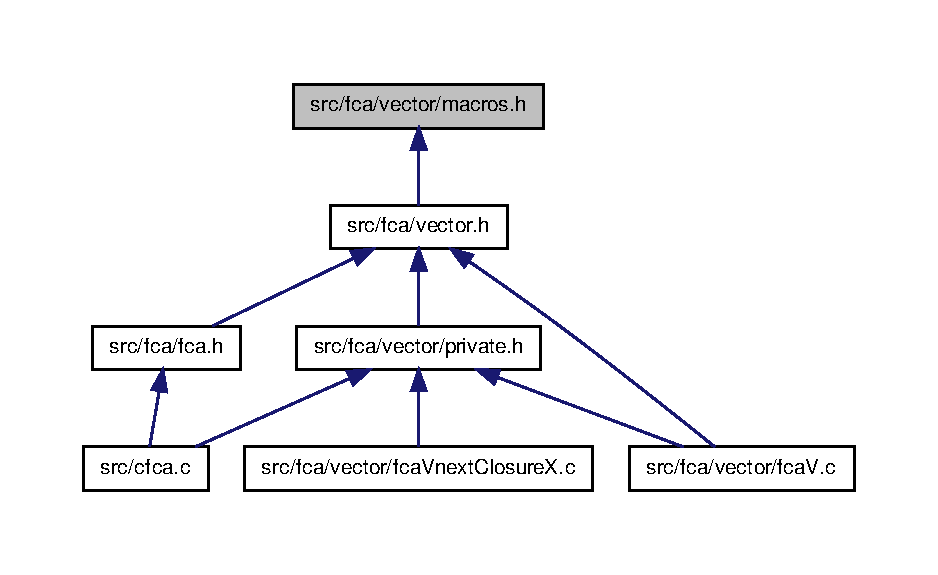
\includegraphics[width=350pt]{vector_2macros_8h__dep__incl}
\end{center}
\end{figure}
\subsection*{\-Defines}
\begin{DoxyCompactItemize}
\item 
\#define \hyperlink{vector_2macros_8h_ad12dce0a7bf9d908b172a28155b3d261}{\-O\-F\-F\-S\-E\-T}(x)~((unsigned)(x)$>$$>$6)
\begin{DoxyCompactList}\small\item\em get the offset of the x-\/th bit in an 64-\/bit integer vector \end{DoxyCompactList}\item 
\#define \hyperlink{vector_2macros_8h_ada941e79b743a29c3b14ead69beacc73}{\-B\-I\-T\-N\-B\-R}(x)~(((unsigned)(x))\&(63))
\begin{DoxyCompactList}\small\item\em get the remainder of the x-\/th bit in an 64-\/bit integer vector, i.\-e. \end{DoxyCompactList}\item 
\#define \hyperlink{vector_2macros_8h_a9978c9be0f4161638ec49b4eda697d42}{\-W\-I\-D\-T\-H}(x)~((((unsigned)(x))\&(63))?((unsigned)(x)/64)+1\-:((unsigned)(x)/64))
\begin{DoxyCompactList}\small\item\em determine the length of an 64-\/bit integer vector that can hold x bits \end{DoxyCompactList}\item 
\#define \hyperlink{vector_2macros_8h_a49be24608e8de0f8bfdf9f69c2a96784}{\-B\-I\-T\-V\-A\-L\-U\-E}(x)~((1\-U\-L\-L$<$$<$(63-\/\-B\-I\-T\-N\-B\-R(x))))
\begin{DoxyCompactList}\small\item\em gives the bit-\/value of the x-\/th bit. \end{DoxyCompactList}\item 
\#define \hyperlink{vector_2macros_8h_af742dc579c934e600fb6a954a4cde678}{\-C\-R\-I\-M\-P\-V\-A\-L\-U\-E}(x)~(($\sim$(0\-U\-L\-L))$>$$>$(63-\/(\-B\-I\-T\-N\-B\-R(x)))$<$$<$(63-\/\-B\-I\-T\-N\-B\-R(x)))
\begin{DoxyCompactList}\small\item\em gives an 64-\/bit integer that has set the bits 0 through x. \end{DoxyCompactList}\item 
\#define \hyperlink{vector_2macros_8h_aef2d7de0c2b6bb72a552503770da6cae}{\-M\-A\-S\-K\-V\-E\-C\-T\-O\-R}(v, x)~\{if (\hyperlink{vector_2macros_8h_ada941e79b743a29c3b14ead69beacc73}{\-B\-I\-T\-N\-B\-R}((x))) \{ $\ast$((v)+\hyperlink{vector_2macros_8h_ad12dce0a7bf9d908b172a28155b3d261}{\-O\-F\-F\-S\-E\-T}((x)-\/1)) = ( ($\ast$((v)+\hyperlink{vector_2macros_8h_ad12dce0a7bf9d908b172a28155b3d261}{\-O\-F\-F\-S\-E\-T}((x)-\/1))$>$$>$(63-\/\hyperlink{vector_2macros_8h_ada941e79b743a29c3b14ead69beacc73}{\-B\-I\-T\-N\-B\-R}((x)-\/1))) ) $<$$<$ (63-\/\hyperlink{vector_2macros_8h_ada941e79b743a29c3b14ead69beacc73}{\-B\-I\-T\-N\-B\-R}((x)-\/1));  \}\}
\begin{DoxyCompactList}\small\item\em set the unused attribute bits to zero. \end{DoxyCompactList}\item 
\#define \hyperlink{vector_2macros_8h_aad0e5eaea1cfebf54257dc40ea185ed4}{\-C\-R\-O\-S\-S\-V}(v, x)~\{ $\ast$((v)+\hyperlink{vector_2macros_8h_ad12dce0a7bf9d908b172a28155b3d261}{\-O\-F\-F\-S\-E\-T}(x)) $|$= \hyperlink{vector_2macros_8h_a49be24608e8de0f8bfdf9f69c2a96784}{\-B\-I\-T\-V\-A\-L\-U\-E}(x); \}
\begin{DoxyCompactList}\small\item\em crosses the x-\/th attribute of an attribute vector \end{DoxyCompactList}\item 
\#define \hyperlink{vector_2macros_8h_a2e3ae6676ab924d72728a1b5d61ea297}{\-C\-L\-E\-A\-R\-V}(v, x)~\{ $\ast$((v)+\hyperlink{vector_2macros_8h_ad12dce0a7bf9d908b172a28155b3d261}{\-O\-F\-F\-S\-E\-T}(x)) \&= $\sim$ (\hyperlink{vector_2macros_8h_a49be24608e8de0f8bfdf9f69c2a96784}{\-B\-I\-T\-V\-A\-L\-U\-E}(x)); \}
\begin{DoxyCompactList}\small\item\em clears the x-\/th attribute of an attribute vector \end{DoxyCompactList}\item 
\#define \hyperlink{vector_2macros_8h_aee89242eec49a02707fd80427af50d23}{\-I\-N\-C\-I\-D\-E\-S\-V}(v, x)~(  ( $\ast$((v)+\hyperlink{vector_2macros_8h_ad12dce0a7bf9d908b172a28155b3d261}{\-O\-F\-F\-S\-E\-T}(x)) $>$$>$ (63-\/\hyperlink{vector_2macros_8h_ada941e79b743a29c3b14ead69beacc73}{\-B\-I\-T\-N\-B\-R}(x)) ) \& 1  )
\begin{DoxyCompactList}\small\item\em checks whether the x-\/th attribute of an attribute vector is crossed \end{DoxyCompactList}\item 
\#define \hyperlink{vector_2macros_8h_a9726c8302995a7cfcb79221354ef69b3}{\-R\-O\-W}(g, \-I)~((\-I)-\/$>$incidence + ((\-I)-\/$>$width $\ast$ (g)))
\begin{DoxyCompactList}\small\item\em gives the attribute vector for a given object \end{DoxyCompactList}\end{DoxyCompactItemize}


\subsection{\-Detailed \-Description}
\hyperlink{vector_2macros_8h}{vector/macros.\-h}, (c) 2013, \-Immanuel \-Albrecht; \-Dresden \-University of \-Technology, \-Professur für die \-Psychologie des \-Lernen und \-Lehrens \-This program is free software\-: you can redistribute it and/or modify it under the terms of the \-G\-N\-U \-General \-Public \-License as published by the \-Free \-Software \-Foundation, either version 3 of the \-License, or (at your option) any later version.

\-This program is distributed in the hope that it will be useful, but \-W\-I\-T\-H\-O\-U\-T \-A\-N\-Y \-W\-A\-R\-R\-A\-N\-T\-Y; without even the implied warranty of \-M\-E\-R\-C\-H\-A\-N\-T\-A\-B\-I\-L\-I\-T\-Y or \-F\-I\-T\-N\-E\-S\-S \-F\-O\-R \-A \-P\-A\-R\-T\-I\-C\-U\-L\-A\-R \-P\-U\-R\-P\-O\-S\-E. \-See the \-G\-N\-U \-General \-Public \-License for more details.

\-You should have received a copy of the \-G\-N\-U \-General \-Public \-License along with this program. \-If not, see $<$\href{http://www.gnu.org/licenses/}{\tt http\-://www.\-gnu.\-org/licenses/}$>$. \-These macros are used for uint64\-\_\-t bit-\/stream arrays 

\-Definition in file \hyperlink{vector_2macros_8h_source}{macros.\-h}.



\subsection{\-Define \-Documentation}
\hypertarget{vector_2macros_8h_ada941e79b743a29c3b14ead69beacc73}{\index{vector/macros.\-h@{vector/macros.\-h}!\-B\-I\-T\-N\-B\-R@{\-B\-I\-T\-N\-B\-R}}
\index{\-B\-I\-T\-N\-B\-R@{\-B\-I\-T\-N\-B\-R}!vector/macros.h@{vector/macros.\-h}}
\subsubsection[{\-B\-I\-T\-N\-B\-R}]{\setlength{\rightskip}{0pt plus 5cm}\#define {\bf \-B\-I\-T\-N\-B\-R}(
\begin{DoxyParamCaption}
\item[{}]{x}
\end{DoxyParamCaption}
)~(((unsigned)(x))\&(63))}}\label{vector_2macros_8h_ada941e79b743a29c3b14ead69beacc73}


get the remainder of the x-\/th bit in an 64-\/bit integer vector, i.\-e. 

65=64+ {\itshape 1\/} 

\-Definition at line 39 of file macros.\-h.



\-Referenced by intent\-Cmp\-V().

\hypertarget{vector_2macros_8h_a49be24608e8de0f8bfdf9f69c2a96784}{\index{vector/macros.\-h@{vector/macros.\-h}!\-B\-I\-T\-V\-A\-L\-U\-E@{\-B\-I\-T\-V\-A\-L\-U\-E}}
\index{\-B\-I\-T\-V\-A\-L\-U\-E@{\-B\-I\-T\-V\-A\-L\-U\-E}!vector/macros.h@{vector/macros.\-h}}
\subsubsection[{\-B\-I\-T\-V\-A\-L\-U\-E}]{\setlength{\rightskip}{0pt plus 5cm}\#define {\bf \-B\-I\-T\-V\-A\-L\-U\-E}(
\begin{DoxyParamCaption}
\item[{}]{x}
\end{DoxyParamCaption}
)~((1\-U\-L\-L$<$$<$(63-\/\-B\-I\-T\-N\-B\-R(x))))}}\label{vector_2macros_8h_a49be24608e8de0f8bfdf9f69c2a96784}


gives the bit-\/value of the x-\/th bit. 

(\-Note that bit 0 is the most, and bit 63 is the least significant bit) 

\-Definition at line 55 of file macros.\-h.

\hypertarget{vector_2macros_8h_a2e3ae6676ab924d72728a1b5d61ea297}{\index{vector/macros.\-h@{vector/macros.\-h}!\-C\-L\-E\-A\-R\-V@{\-C\-L\-E\-A\-R\-V}}
\index{\-C\-L\-E\-A\-R\-V@{\-C\-L\-E\-A\-R\-V}!vector/macros.h@{vector/macros.\-h}}
\subsubsection[{\-C\-L\-E\-A\-R\-V}]{\setlength{\rightskip}{0pt plus 5cm}\#define {\bf \-C\-L\-E\-A\-R\-V}(
\begin{DoxyParamCaption}
\item[{}]{v, }
\item[{}]{x}
\end{DoxyParamCaption}
)~\{ $\ast$((v)+{\bf \-O\-F\-F\-S\-E\-T}(x)) \&= $\sim$ ({\bf \-B\-I\-T\-V\-A\-L\-U\-E}(x)); \}}}\label{vector_2macros_8h_a2e3ae6676ab924d72728a1b5d61ea297}


clears the x-\/th attribute of an attribute vector 



\-Definition at line 108 of file macros.\-h.



\-Referenced by count\-Context\-Concepts\-V(), new\-Concept\-Bulk\-From\-Context\-V(), and next\-Closure\-V\-X1().

\hypertarget{vector_2macros_8h_af742dc579c934e600fb6a954a4cde678}{\index{vector/macros.\-h@{vector/macros.\-h}!\-C\-R\-I\-M\-P\-V\-A\-L\-U\-E@{\-C\-R\-I\-M\-P\-V\-A\-L\-U\-E}}
\index{\-C\-R\-I\-M\-P\-V\-A\-L\-U\-E@{\-C\-R\-I\-M\-P\-V\-A\-L\-U\-E}!vector/macros.h@{vector/macros.\-h}}
\subsubsection[{\-C\-R\-I\-M\-P\-V\-A\-L\-U\-E}]{\setlength{\rightskip}{0pt plus 5cm}\#define {\bf \-C\-R\-I\-M\-P\-V\-A\-L\-U\-E}(
\begin{DoxyParamCaption}
\item[{}]{x}
\end{DoxyParamCaption}
)~(($\sim$(0\-U\-L\-L))$>$$>$(63-\/(\-B\-I\-T\-N\-B\-R(x)))$<$$<$(63-\/\-B\-I\-T\-N\-B\-R(x)))}}\label{vector_2macros_8h_af742dc579c934e600fb6a954a4cde678}


gives an 64-\/bit integer that has set the bits 0 through x. 

\hyperlink{vector_2macros_8h_af742dc579c934e600fb6a954a4cde678}{\-C\-R\-I\-M\-P\-V\-A\-L\-U\-E(0)} == 0x8000000000000000 \hyperlink{vector_2macros_8h_af742dc579c934e600fb6a954a4cde678}{\-C\-R\-I\-M\-P\-V\-A\-L\-U\-E(1)} == 0xc000000000000000 \hyperlink{vector_2macros_8h_af742dc579c934e600fb6a954a4cde678}{\-C\-R\-I\-M\-P\-V\-A\-L\-U\-E(2)} == 0xe000000000000000 \hyperlink{vector_2macros_8h_af742dc579c934e600fb6a954a4cde678}{\-C\-R\-I\-M\-P\-V\-A\-L\-U\-E(3)} == 0xf000000000000000 \hyperlink{vector_2macros_8h_af742dc579c934e600fb6a954a4cde678}{\-C\-R\-I\-M\-P\-V\-A\-L\-U\-E(4)} == 0xf800000000000000 etc. 

\-Definition at line 77 of file macros.\-h.



\-Referenced by count\-Context\-Concepts\-V(), intent\-Cmp\-V(), new\-Concept\-Bulk\-From\-Context\-V(), and next\-Closure\-V\-X1().

\hypertarget{vector_2macros_8h_aad0e5eaea1cfebf54257dc40ea185ed4}{\index{vector/macros.\-h@{vector/macros.\-h}!\-C\-R\-O\-S\-S\-V@{\-C\-R\-O\-S\-S\-V}}
\index{\-C\-R\-O\-S\-S\-V@{\-C\-R\-O\-S\-S\-V}!vector/macros.h@{vector/macros.\-h}}
\subsubsection[{\-C\-R\-O\-S\-S\-V}]{\setlength{\rightskip}{0pt plus 5cm}\#define {\bf \-C\-R\-O\-S\-S\-V}(
\begin{DoxyParamCaption}
\item[{}]{v, }
\item[{}]{x}
\end{DoxyParamCaption}
)~\{ $\ast$((v)+{\bf \-O\-F\-F\-S\-E\-T}(x)) $|$= {\bf \-B\-I\-T\-V\-A\-L\-U\-E}(x); \}}}\label{vector_2macros_8h_aad0e5eaea1cfebf54257dc40ea185ed4}


crosses the x-\/th attribute of an attribute vector 



\-Definition at line 102 of file macros.\-h.



\-Referenced by count\-Context\-Concepts\-V(), new\-Concept\-Bulk\-From\-Context\-V(), new\-Formal\-Context\-From\-File\-V(), next\-Closure\-V\-X(), and next\-Closure\-V\-X1().

\hypertarget{vector_2macros_8h_aee89242eec49a02707fd80427af50d23}{\index{vector/macros.\-h@{vector/macros.\-h}!\-I\-N\-C\-I\-D\-E\-S\-V@{\-I\-N\-C\-I\-D\-E\-S\-V}}
\index{\-I\-N\-C\-I\-D\-E\-S\-V@{\-I\-N\-C\-I\-D\-E\-S\-V}!vector/macros.h@{vector/macros.\-h}}
\subsubsection[{\-I\-N\-C\-I\-D\-E\-S\-V}]{\setlength{\rightskip}{0pt plus 5cm}\#define {\bf \-I\-N\-C\-I\-D\-E\-S\-V}(
\begin{DoxyParamCaption}
\item[{}]{v, }
\item[{}]{x}
\end{DoxyParamCaption}
)~(  ( $\ast$((v)+{\bf \-O\-F\-F\-S\-E\-T}(x)) $>$$>$ (63-\/{\bf \-B\-I\-T\-N\-B\-R}(x)) ) \& 1  )}}\label{vector_2macros_8h_aee89242eec49a02707fd80427af50d23}


checks whether the x-\/th attribute of an attribute vector is crossed 



\-Definition at line 114 of file macros.\-h.



\-Referenced by count\-Context\-Concepts\-V(), new\-Concept\-Bulk\-From\-Context\-V(), next\-Closure\-V\-X1(), write\-Concepts\-To\-File\-V(), and write\-Formal\-Context\-V().

\hypertarget{vector_2macros_8h_aef2d7de0c2b6bb72a552503770da6cae}{\index{vector/macros.\-h@{vector/macros.\-h}!\-M\-A\-S\-K\-V\-E\-C\-T\-O\-R@{\-M\-A\-S\-K\-V\-E\-C\-T\-O\-R}}
\index{\-M\-A\-S\-K\-V\-E\-C\-T\-O\-R@{\-M\-A\-S\-K\-V\-E\-C\-T\-O\-R}!vector/macros.h@{vector/macros.\-h}}
\subsubsection[{\-M\-A\-S\-K\-V\-E\-C\-T\-O\-R}]{\setlength{\rightskip}{0pt plus 5cm}\#define {\bf \-M\-A\-S\-K\-V\-E\-C\-T\-O\-R}(
\begin{DoxyParamCaption}
\item[{}]{v, }
\item[{}]{x}
\end{DoxyParamCaption}
)~\{if ({\bf \-B\-I\-T\-N\-B\-R}((x))) \{ $\ast$((v)+{\bf \-O\-F\-F\-S\-E\-T}((x)-\/1)) = ( ($\ast$((v)+{\bf \-O\-F\-F\-S\-E\-T}((x)-\/1))$>$$>$(63-\/{\bf \-B\-I\-T\-N\-B\-R}((x)-\/1))) ) $<$$<$ (63-\/{\bf \-B\-I\-T\-N\-B\-R}((x)-\/1));  \}\}}}\label{vector_2macros_8h_aef2d7de0c2b6bb72a552503770da6cae}


set the unused attribute bits to zero. 

(i.\-e. attributes == 100 -\/$>$ width == 2, \hyperlink{vector_2macros_8h_ada941e79b743a29c3b14ead69beacc73}{\-B\-I\-T\-N\-B\-R(99)} == 35) where v is a 64-\/bit integer vector, and x is the number used bits. 

\-Definition at line 91 of file macros.\-h.



\-Referenced by close\-Intent\-V().

\hypertarget{vector_2macros_8h_ad12dce0a7bf9d908b172a28155b3d261}{\index{vector/macros.\-h@{vector/macros.\-h}!\-O\-F\-F\-S\-E\-T@{\-O\-F\-F\-S\-E\-T}}
\index{\-O\-F\-F\-S\-E\-T@{\-O\-F\-F\-S\-E\-T}!vector/macros.h@{vector/macros.\-h}}
\subsubsection[{\-O\-F\-F\-S\-E\-T}]{\setlength{\rightskip}{0pt plus 5cm}\#define {\bf \-O\-F\-F\-S\-E\-T}(
\begin{DoxyParamCaption}
\item[{}]{x}
\end{DoxyParamCaption}
)~((unsigned)(x)$>$$>$6)}}\label{vector_2macros_8h_ad12dce0a7bf9d908b172a28155b3d261}


get the offset of the x-\/th bit in an 64-\/bit integer vector 



\-Definition at line 33 of file macros.\-h.



\-Referenced by count\-Context\-Concepts\-V(), intent\-Cmp\-V(), new\-Concept\-Bulk\-From\-Context\-V(), and next\-Closure\-V\-X1().

\hypertarget{vector_2macros_8h_a9726c8302995a7cfcb79221354ef69b3}{\index{vector/macros.\-h@{vector/macros.\-h}!\-R\-O\-W@{\-R\-O\-W}}
\index{\-R\-O\-W@{\-R\-O\-W}!vector/macros.h@{vector/macros.\-h}}
\subsubsection[{\-R\-O\-W}]{\setlength{\rightskip}{0pt plus 5cm}\#define {\bf \-R\-O\-W}(
\begin{DoxyParamCaption}
\item[{}]{g, }
\item[{}]{\-I}
\end{DoxyParamCaption}
)~((\-I)-\/$>$incidence + ((\-I)-\/$>$width $\ast$ (g)))}}\label{vector_2macros_8h_a9726c8302995a7cfcb79221354ef69b3}


gives the attribute vector for a given object 



\-Definition at line 125 of file macros.\-h.



\-Referenced by add\-Concept\-To\-Bulk\-V(), close\-Intent\-V(), new\-Formal\-Context\-From\-File\-V(), write\-Concepts\-To\-File\-V(), and write\-Formal\-Context\-V().

\hypertarget{vector_2macros_8h_a9978c9be0f4161638ec49b4eda697d42}{\index{vector/macros.\-h@{vector/macros.\-h}!\-W\-I\-D\-T\-H@{\-W\-I\-D\-T\-H}}
\index{\-W\-I\-D\-T\-H@{\-W\-I\-D\-T\-H}!vector/macros.h@{vector/macros.\-h}}
\subsubsection[{\-W\-I\-D\-T\-H}]{\setlength{\rightskip}{0pt plus 5cm}\#define {\bf \-W\-I\-D\-T\-H}(
\begin{DoxyParamCaption}
\item[{}]{x}
\end{DoxyParamCaption}
)~((((unsigned)(x))\&(63))?((unsigned)(x)/64)+1\-:((unsigned)(x)/64))}}\label{vector_2macros_8h_a9978c9be0f4161638ec49b4eda697d42}


determine the length of an 64-\/bit integer vector that can hold x bits 



\-Definition at line 46 of file macros.\-h.



\-Referenced by new\-Concept\-Bulk\-V(), new\-Concept\-Chunk\-V(), and new\-Formal\-Context\-V().


\hypertarget{common_2measurement_8c}{\section{src/fca/common/measurement.c \-File \-Reference}
\label{common_2measurement_8c}\index{src/fca/common/measurement.\-c@{src/fca/common/measurement.\-c}}
}


measurement.\-c, (c) 2013, \-Immanuel \-Albrecht; \-Dresden \-University of \-Technology, \-Professur für die \-Psychologie des \-Lernen und \-Lehrens  


{\ttfamily \#include $<$math.\-h$>$}\*
{\ttfamily \#include $<$string.\-h$>$}\*
{\ttfamily \#include \char`\"{}../common.\-h\char`\"{}}\*
\-Include dependency graph for measurement.\-c\-:\nopagebreak
\begin{figure}[H]
\begin{center}
\leavevmode
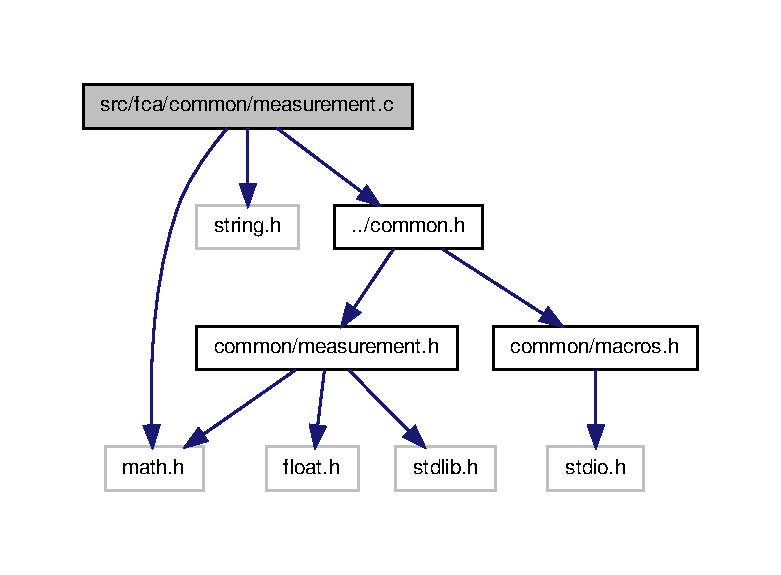
\includegraphics[width=350pt]{common_2measurement_8c__incl}
\end{center}
\end{figure}
\subsection*{\-Functions}
\begin{DoxyCompactItemize}
\item 
\hyperlink{common_2measurement_8h_ab2406aaef0ce3e9f38a79f42ce470ffb}{\-Eta\-Function} \hyperlink{common_2measurement_8c_aa0f12091b86c478e159761719923bd9a}{new\-Eta\-Function} (size\-\_\-t types, size\-\_\-t measurements, size\-\_\-t constants)
\begin{DoxyCompactList}\small\item\em creates a new \-Eta\-Function \end{DoxyCompactList}\item 
void \hyperlink{common_2measurement_8c_a2905b59d4a364111890224a444fd6d30}{delete\-Eta\-Function} (\hyperlink{common_2measurement_8h_ab2406aaef0ce3e9f38a79f42ce470ffb}{\-Eta\-Function} $\ast$eta)
\begin{DoxyCompactList}\small\item\em deletes an \-Eta\-Function and sets the pointer to zero \end{DoxyCompactList}\item 
\hyperlink{common_2measurement_8h_ab2406aaef0ce3e9f38a79f42ce470ffb}{\-Eta\-Function} \hyperlink{common_2measurement_8c_a48c795067056a496c8e4aa903fac7d71}{new\-Uniform\-Eta\-Function} (size\-\_\-t types, size\-\_\-t measurements)
\begin{DoxyCompactList}\small\item\em create a new \-Eta\-Function with the same constant for each type \end{DoxyCompactList}\item 
\hyperlink{common_2measurement_8h_ab2406aaef0ce3e9f38a79f42ce470ffb}{\-Eta\-Function} \hyperlink{common_2measurement_8c_a018a3a7d15c126cbf15d03ba2698fe39}{new\-General\-Eta\-Function} (size\-\_\-t types, size\-\_\-t measurements)
\begin{DoxyCompactList}\small\item\em create a new \-Eta\-Function with the a constant for each type and measurement on its own \end{DoxyCompactList}\item 
\hyperlink{common_2measurement_8h_afb8ffb8c068ef8c9fa3677762ac85994}{\-Commutative\-Product} \hyperlink{common_2measurement_8c_abe35a2e2ccf6060635d4daf6d6ebf59e}{new\-Commutative\-Product} (size\-\_\-t constants)
\begin{DoxyCompactList}\small\item\em creates a new commutative product without any factors \end{DoxyCompactList}\item 
void \hyperlink{common_2measurement_8c_a2120fbc047167fd0a08f3015b8716cd1}{delete\-Commutative\-Product} (\hyperlink{common_2measurement_8h_afb8ffb8c068ef8c9fa3677762ac85994}{\-Commutative\-Product} $\ast$p)
\begin{DoxyCompactList}\small\item\em deletes a \-Commutative\-Product and sets its pointer to zero. \end{DoxyCompactList}\item 
\hyperlink{common_2measurement_8h_ab2f71cb9d9b10edcc10d44f79ee40d10}{\-Condition\-Map} \hyperlink{common_2measurement_8c_ac4b7705e5a5c82b5d59b67617e6f2dc4}{new\-Condition\-Map} (size\-\_\-t objects)
\begin{DoxyCompactList}\small\item\em creates a new condition map \end{DoxyCompactList}\item 
void \hyperlink{common_2measurement_8c_ad40c601ad1dcd904cde0e9ebe2828d72}{delete\-Condition\-Map} (\hyperlink{common_2measurement_8h_ab2f71cb9d9b10edcc10d44f79ee40d10}{\-Condition\-Map} $\ast$c)
\begin{DoxyCompactList}\small\item\em deletes a \-Condition\-Map object \end{DoxyCompactList}\item 
\hyperlink{common_2measurement_8h_ace94e4c4dddc7766492a0f041a72963b}{\-Log\-Cache} \hyperlink{common_2measurement_8c_a25fcd9b89607eaa3abe03aea6ffe0447}{new\-Log\-Cache} (size\-\_\-t constants)
\begin{DoxyCompactList}\small\item\em creates a new cache for logs of constants \end{DoxyCompactList}\item 
void \hyperlink{common_2measurement_8c_ae9d17380c2a4280b6760d9d917dfb573}{delete\-Log\-Cache} (\hyperlink{common_2measurement_8h_ace94e4c4dddc7766492a0f041a72963b}{\-Log\-Cache} $\ast$log\-\_\-c)
\begin{DoxyCompactList}\small\item\em deletes a \-Log\-Cache and sets its pointer to zero \end{DoxyCompactList}\item 
void \hyperlink{common_2measurement_8c_aea95ce7469fb27ec5a2fa98d099df572}{calculate\-Logs} (const \hyperlink{common_2measurement_8h_ab2406aaef0ce3e9f38a79f42ce470ffb}{\-Eta\-Function} eta, \hyperlink{common_2measurement_8h_ace94e4c4dddc7766492a0f041a72963b}{\-Log\-Cache} log\-\_\-c)
\begin{DoxyCompactList}\small\item\em calculates the logarithms of probabilities given by constants, and their complements \end{DoxyCompactList}\item 
\hyperlink{common_2measurement_8h_a0a02860cc83aa9ce63d00855bc9058e0}{\-Log\-Probability} \hyperlink{common_2measurement_8c_a8df411530d5811c51cb675a64547eed9}{log\-Probability\-From\-Product} (const \hyperlink{common_2measurement_8h_ace94e4c4dddc7766492a0f041a72963b}{\-Log\-Cache} log\-\_\-c, \hyperlink{common_2measurement_8h_afb8ffb8c068ef8c9fa3677762ac85994}{\-Commutative\-Product} l)
\begin{DoxyCompactList}\small\item\em calculate the log probability from a power vector \end{DoxyCompactList}\item 
\hyperlink{common_2measurement_8h_a0a02860cc83aa9ce63d00855bc9058e0}{\-Log\-Probability} \hyperlink{common_2measurement_8c_a6ec39ef8a7180bc340afed87c57ca604}{sum\-Up} (const \hyperlink{common_2measurement_8h_a0a02860cc83aa9ce63d00855bc9058e0}{\-Log\-Probability} $\ast$restrict \-V, size\-\_\-t length, \hyperlink{common_2measurement_8h_a0a02860cc83aa9ce63d00855bc9058e0}{\-Log\-Probability} lower\-\_\-bound, \hyperlink{common_2measurement_8h_a0a02860cc83aa9ce63d00855bc9058e0}{\-Log\-Probability} upper\-\_\-bound)
\begin{DoxyCompactList}\small\item\em \-This routine calculates the sum of elements of a vector. \end{DoxyCompactList}\item 
\hyperlink{common_2measurement_8h_a315318def4482768da7077f76ff0c768}{\-Distance\-Matrix} \hyperlink{common_2measurement_8c_ae6570aaa925f8a9155f9385de467dcbd}{new\-Distance\-Matrix} (size\-\_\-t objects)
\begin{DoxyCompactList}\small\item\em creates a new \-Distance\-Matrix of the given size \end{DoxyCompactList}\item 
void \hyperlink{common_2measurement_8c_a573c3990ed39b5ca911c9ef448f74703}{delete\-Distance\-Matrix} (\hyperlink{common_2measurement_8h_a315318def4482768da7077f76ff0c768}{\-Distance\-Matrix} $\ast$d)
\begin{DoxyCompactList}\small\item\em deletes the given object and sets its pointer to zero \end{DoxyCompactList}\item 
void \hyperlink{common_2measurement_8c_ad54d95f7de71efa2ad16ce6b133cf439}{write\-Distances\-To\-File} (const \hyperlink{common_2measurement_8h_a315318def4482768da7077f76ff0c768}{\-Distance\-Matrix} d, const char $\ast$filename)
\begin{DoxyCompactList}\small\item\em \-Writes the contents of a distance matrix to the given file in \-C\-S\-V format\-: d(x,y) will be written on the (x+1)th line to the (y+1)th column. \end{DoxyCompactList}\item 
void \hyperlink{common_2measurement_8c_a6441c79f9d24d9b47cf21dc69ab7638b}{normalize\-Distance\-Matrix} (\hyperlink{common_2measurement_8h_a315318def4482768da7077f76ff0c768}{\-Distance\-Matrix} restrict d)
\begin{DoxyCompactList}\small\item\em normalizes the distance matrix by replacing d with d', which is defined to be \end{DoxyCompactList}\end{DoxyCompactItemize}


\subsection{\-Detailed \-Description}
measurement.\-c, (c) 2013, \-Immanuel \-Albrecht; \-Dresden \-University of \-Technology, \-Professur für die \-Psychologie des \-Lernen und \-Lehrens \-This program is free software\-: you can redistribute it and/or modify it under the terms of the \-G\-N\-U \-General \-Public \-License as published by the \-Free \-Software \-Foundation, either version 3 of the \-License, or (at your option) any later version.

\-This program is distributed in the hope that it will be useful, but \-W\-I\-T\-H\-O\-U\-T \-A\-N\-Y \-W\-A\-R\-R\-A\-N\-T\-Y; without even the implied warranty of \-M\-E\-R\-C\-H\-A\-N\-T\-A\-B\-I\-L\-I\-T\-Y or \-F\-I\-T\-N\-E\-S\-S \-F\-O\-R \-A \-P\-A\-R\-T\-I\-C\-U\-L\-A\-R \-P\-U\-R\-P\-O\-S\-E. \-See the \-G\-N\-U \-General \-Public \-License for more details.

\-You should have received a copy of the \-G\-N\-U \-General \-Public \-License along with this program. \-If not, see $<$\href{http://www.gnu.org/licenses/}{\tt http\-://www.\-gnu.\-org/licenses/}$>$. \-This file contains implementations regarding measurement error probabilities related structures operations 

\-Definition in file \hyperlink{common_2measurement_8c_source}{measurement.\-c}.



\subsection{\-Function \-Documentation}
\hypertarget{common_2measurement_8c_aea95ce7469fb27ec5a2fa98d099df572}{\index{common/measurement.\-c@{common/measurement.\-c}!calculate\-Logs@{calculate\-Logs}}
\index{calculate\-Logs@{calculate\-Logs}!common/measurement.c@{common/measurement.\-c}}
\subsubsection[{calculate\-Logs}]{\setlength{\rightskip}{0pt plus 5cm}void {\bf calculate\-Logs} (
\begin{DoxyParamCaption}
\item[{const {\bf \-Eta\-Function}}]{eta, }
\item[{{\bf \-Log\-Cache}}]{log\-\_\-c}
\end{DoxyParamCaption}
)}}\label{common_2measurement_8c_aea95ce7469fb27ec5a2fa98d099df572}


calculates the logarithms of probabilities given by constants, and their complements 


\begin{DoxyParams}{\-Parameters}
{\em eta} & input constants \\
\hline
{\em log\-\_\-c} & output structure to update the constants \\
\hline
\end{DoxyParams}


\-Definition at line 239 of file measurement.\-c.



\-References s\-Eta\-Function\-::\-C, s\-Eta\-Function\-::constants, s\-Log\-Cache\-::constants, s\-Log\-Cache\-::log\-C, s\-Log\-Cache\-::log\-Not\-C, and \-W\-A\-R\-N\-\_\-\-I\-F\-\_\-\-U\-N\-E\-Q\-U\-A\-L\-\_\-\-D\-O.



\-Referenced by main().


\begin{DoxyCode}
{
    WARN_IF_UNEQUAL_DO(eta->constants, log_c->constants, return);

    /*
     * we could use just any logarithm, so 2 seems reasonable...
     */

    for (size_t i = 0; i < eta->constants; ++i)
    {
        log_c->logC[i] = log2(eta->C[i]);
        log_c->logNotC[i] = log2(1. - eta->C[i]);
    }
}
\end{DoxyCode}
\hypertarget{common_2measurement_8c_a2120fbc047167fd0a08f3015b8716cd1}{\index{common/measurement.\-c@{common/measurement.\-c}!delete\-Commutative\-Product@{delete\-Commutative\-Product}}
\index{delete\-Commutative\-Product@{delete\-Commutative\-Product}!common/measurement.c@{common/measurement.\-c}}
\subsubsection[{delete\-Commutative\-Product}]{\setlength{\rightskip}{0pt plus 5cm}void {\bf delete\-Commutative\-Product} (
\begin{DoxyParamCaption}
\item[{{\bf \-Commutative\-Product} $\ast$}]{p}
\end{DoxyParamCaption}
)}}\label{common_2measurement_8c_a2120fbc047167fd0a08f3015b8716cd1}


deletes a \-Commutative\-Product and sets its pointer to zero. 


\begin{DoxyParams}{\-Parameters}
{\em p} & \\
\hline
\end{DoxyParams}


\-Definition at line 149 of file measurement.\-c.



\-References \-R\-E\-T\-U\-R\-N\-\_\-\-I\-F\-\_\-\-Z\-E\-R\-O.



\-Referenced by new\-Distance\-Matrix\-From\-Context(), optimize\-Approximation\-Context(), and optimize\-Condition\-Map().


\begin{DoxyCode}
{
    RETURN_IF_ZERO(p);
    RETURN_IF_ZERO(*p);

    free((*p)->match);
    free((*p)->mismatch);
    free((*p)->intermediate);
    free(*p);

    *p = 0;
}
\end{DoxyCode}
\hypertarget{common_2measurement_8c_ad40c601ad1dcd904cde0e9ebe2828d72}{\index{common/measurement.\-c@{common/measurement.\-c}!delete\-Condition\-Map@{delete\-Condition\-Map}}
\index{delete\-Condition\-Map@{delete\-Condition\-Map}!common/measurement.c@{common/measurement.\-c}}
\subsubsection[{delete\-Condition\-Map}]{\setlength{\rightskip}{0pt plus 5cm}void {\bf delete\-Condition\-Map} (
\begin{DoxyParamCaption}
\item[{{\bf \-Condition\-Map} $\ast$}]{c}
\end{DoxyParamCaption}
)}}\label{common_2measurement_8c_ad40c601ad1dcd904cde0e9ebe2828d72}


deletes a \-Condition\-Map object 


\begin{DoxyParams}{\-Parameters}
{\em c} & \\
\hline
\end{DoxyParams}


\-Definition at line 186 of file measurement.\-c.



\-References \-R\-E\-T\-U\-R\-N\-\_\-\-I\-F\-\_\-\-Z\-E\-R\-O.



\-Referenced by main().


\begin{DoxyCode}
{
    RETURN_IF_ZERO(c);
    RETURN_IF_ZERO(*c);

    free((*c)->c);
    free(*c);

    *c = 0;
}
\end{DoxyCode}
\hypertarget{common_2measurement_8c_a573c3990ed39b5ca911c9ef448f74703}{\index{common/measurement.\-c@{common/measurement.\-c}!delete\-Distance\-Matrix@{delete\-Distance\-Matrix}}
\index{delete\-Distance\-Matrix@{delete\-Distance\-Matrix}!common/measurement.c@{common/measurement.\-c}}
\subsubsection[{delete\-Distance\-Matrix}]{\setlength{\rightskip}{0pt plus 5cm}void {\bf delete\-Distance\-Matrix} (
\begin{DoxyParamCaption}
\item[{{\bf \-Distance\-Matrix} $\ast$}]{d}
\end{DoxyParamCaption}
)}}\label{common_2measurement_8c_a573c3990ed39b5ca911c9ef448f74703}


deletes the given object and sets its pointer to zero 


\begin{DoxyParams}{\-Parameters}
{\em d} & \-Distance\-Matrix \\
\hline
\end{DoxyParams}


\-Definition at line 357 of file measurement.\-c.



\-References \-R\-E\-T\-U\-R\-N\-\_\-\-I\-F\-\_\-\-Z\-E\-R\-O.



\-Referenced by main().


\begin{DoxyCode}
{
    RETURN_IF_ZERO(d);

    free((*d)->d);
    free(*d);

    d = 0;
}
\end{DoxyCode}
\hypertarget{common_2measurement_8c_a2905b59d4a364111890224a444fd6d30}{\index{common/measurement.\-c@{common/measurement.\-c}!delete\-Eta\-Function@{delete\-Eta\-Function}}
\index{delete\-Eta\-Function@{delete\-Eta\-Function}!common/measurement.c@{common/measurement.\-c}}
\subsubsection[{delete\-Eta\-Function}]{\setlength{\rightskip}{0pt plus 5cm}void {\bf delete\-Eta\-Function} (
\begin{DoxyParamCaption}
\item[{{\bf \-Eta\-Function} $\ast$}]{eta}
\end{DoxyParamCaption}
)}}\label{common_2measurement_8c_a2905b59d4a364111890224a444fd6d30}


deletes an \-Eta\-Function and sets the pointer to zero 


\begin{DoxyParams}{\-Parameters}
{\em eta} & \\
\hline
\end{DoxyParams}


\-Definition at line 62 of file measurement.\-c.



\-References \-R\-E\-T\-U\-R\-N\-\_\-\-I\-F\-\_\-\-Z\-E\-R\-O.



\-Referenced by main().


\begin{DoxyCode}
{
    RETURN_IF_ZERO(eta);
    RETURN_IF_ZERO(*eta);

    free((*eta)->C);
    free((*eta)->eta);
    free(*eta);

    *eta = 0;
}
\end{DoxyCode}
\hypertarget{common_2measurement_8c_ae9d17380c2a4280b6760d9d917dfb573}{\index{common/measurement.\-c@{common/measurement.\-c}!delete\-Log\-Cache@{delete\-Log\-Cache}}
\index{delete\-Log\-Cache@{delete\-Log\-Cache}!common/measurement.c@{common/measurement.\-c}}
\subsubsection[{delete\-Log\-Cache}]{\setlength{\rightskip}{0pt plus 5cm}void {\bf delete\-Log\-Cache} (
\begin{DoxyParamCaption}
\item[{{\bf \-Log\-Cache} $\ast$}]{log\-\_\-c}
\end{DoxyParamCaption}
)}}\label{common_2measurement_8c_ae9d17380c2a4280b6760d9d917dfb573}


deletes a \-Log\-Cache and sets its pointer to zero 


\begin{DoxyParams}{\-Parameters}
{\em log\-\_\-c} & \\
\hline
\end{DoxyParams}


\-Definition at line 221 of file measurement.\-c.



\-References \-R\-E\-T\-U\-R\-N\-\_\-\-I\-F\-\_\-\-Z\-E\-R\-O.



\-Referenced by main().


\begin{DoxyCode}
{
    RETURN_IF_ZERO(log_c);
    RETURN_IF_ZERO(*log_c);

    free((*log_c)->logC);
    free((*log_c)->logNotC);
    free(*log_c);

    *log_c = 0;
}
\end{DoxyCode}
\hypertarget{common_2measurement_8c_a8df411530d5811c51cb675a64547eed9}{\index{common/measurement.\-c@{common/measurement.\-c}!log\-Probability\-From\-Product@{log\-Probability\-From\-Product}}
\index{log\-Probability\-From\-Product@{log\-Probability\-From\-Product}!common/measurement.c@{common/measurement.\-c}}
\subsubsection[{log\-Probability\-From\-Product}]{\setlength{\rightskip}{0pt plus 5cm}{\bf \-Log\-Probability} {\bf log\-Probability\-From\-Product} (
\begin{DoxyParamCaption}
\item[{const {\bf \-Log\-Cache}}]{log\-\_\-c, }
\item[{{\bf \-Commutative\-Product}}]{l}
\end{DoxyParamCaption}
)}}\label{common_2measurement_8c_a8df411530d5811c51cb675a64547eed9}


calculate the log probability from a power vector 


\begin{DoxyParams}{\-Parameters}
{\em log\-\_\-c} & logarithms of constants \\
\hline
{\em l} & vector of constant and complementary powers \\
\hline
\end{DoxyParams}
\begin{DoxyReturn}{\-Returns}
the log probability of the product given by the vector of powers, l 
\end{DoxyReturn}


\-Definition at line 261 of file measurement.\-c.



\-References s\-Commutative\-Product\-::constants, s\-Log\-Cache\-::constants, s\-Commutative\-Product\-::intermediate, \-L\-O\-G\-\_\-\-P\-R\-O\-B\-\_\-\-L\-O\-W\-E\-R\-\_\-\-B\-O\-U\-N\-D, \-L\-O\-G\-\_\-\-P\-R\-O\-B\-\_\-\-U\-P\-P\-E\-R\-\_\-\-B\-O\-U\-N\-D, s\-Log\-Cache\-::log\-C, s\-Log\-Cache\-::log\-Not\-C, s\-Commutative\-Product\-::match, s\-Commutative\-Product\-::mismatch, \-R\-E\-T\-U\-R\-N\-\_\-\-Z\-E\-R\-O\-\_\-\-I\-F\-\_\-\-Z\-E\-R\-O, sum\-Up(), and \-W\-A\-R\-N\-\_\-\-I\-F\-\_\-\-U\-N\-E\-Q\-U\-A\-L\-\_\-\-D\-O.



\-Referenced by new\-Distance\-Matrix\-From\-Context(), optimize\-Approximation\-Context(), and optimize\-Condition\-Map().


\begin{DoxyCode}
{
    RETURN_ZERO_IF_ZERO(log_c);
    RETURN_ZERO_IF_ZERO(l);

    WARN_IF_UNEQUAL_DO(log_c->constants, l->constants, return 0);
    size_t constants = log_c->constants;

    for (size_t c = 0; c < constants; ++c)
    {
#pragma GCC diagnostic push
#pragma GCC diagnostic ignored "-Wconversion"
        /*
         * 0*-inf is still -inf; but we want to enforce 0*-inf = 0
         */
        if (l->match[c] > 0)
            l->intermediate[c] = log_c->logNotC[c]
                    * (LogProbability) l->match[c];
        else
            l->intermediate[c] = 0.;

        if (l->mismatch[c] > 0)
            l->intermediate[c + constants] = log_c->logC[c]
                    * (LogProbability) l->mismatch[c];
        else
            l->intermediate[c + constants] = 0.;
#pragma GCC diagnostic pop
    }

    return sumUp(l->intermediate, constants * 2, LOG_PROB_LOWER_BOUND,
    LOG_PROB_UPPER_BOUND);
}
\end{DoxyCode}


\-Here is the call graph for this function\-:\nopagebreak
\begin{figure}[H]
\begin{center}
\leavevmode
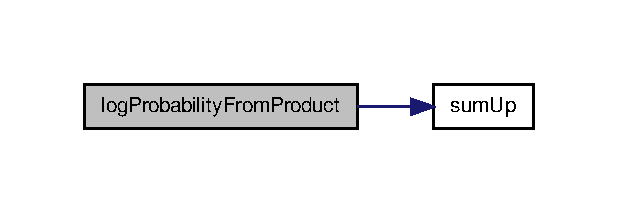
\includegraphics[width=296pt]{common_2measurement_8c_a8df411530d5811c51cb675a64547eed9_cgraph}
\end{center}
\end{figure}


\hypertarget{common_2measurement_8c_abe35a2e2ccf6060635d4daf6d6ebf59e}{\index{common/measurement.\-c@{common/measurement.\-c}!new\-Commutative\-Product@{new\-Commutative\-Product}}
\index{new\-Commutative\-Product@{new\-Commutative\-Product}!common/measurement.c@{common/measurement.\-c}}
\subsubsection[{new\-Commutative\-Product}]{\setlength{\rightskip}{0pt plus 5cm}{\bf \-Commutative\-Product} {\bf new\-Commutative\-Product} (
\begin{DoxyParamCaption}
\item[{size\-\_\-t}]{constants}
\end{DoxyParamCaption}
)}}\label{common_2measurement_8c_abe35a2e2ccf6060635d4daf6d6ebf59e}


creates a new commutative product without any factors 


\begin{DoxyParams}{\-Parameters}
{\em constants} & number of formal constants \\
\hline
\end{DoxyParams}
\begin{DoxyReturn}{\-Returns}
new \-Commutative\-Product object 
\end{DoxyReturn}


\-Definition at line 126 of file measurement.\-c.



\-References s\-Commutative\-Product\-::constants, s\-Commutative\-Product\-::intermediate, s\-Commutative\-Product\-::match, s\-Commutative\-Product\-::mismatch, and \-R\-E\-T\-U\-R\-N\-\_\-\-Z\-E\-R\-O\-\_\-\-I\-F\-\_\-\-Z\-E\-R\-O\-I.



\-Referenced by new\-Distance\-Matrix\-From\-Context(), optimize\-Approximation\-Context(), and optimize\-Condition\-Map().


\begin{DoxyCode}
{
    RETURN_ZERO_IF_ZEROI(constants);

    CommutativeProduct p;
    p = malloc(sizeof(struct sCommutativeProduct));

    p->constants = constants;

    p->mismatch = calloc(constants, sizeof(size_t));
    p->match = calloc(constants, sizeof(size_t));

    p->intermediate = malloc(constants * 2 * sizeof(LogProbability));

    return p;
}
\end{DoxyCode}
\hypertarget{common_2measurement_8c_ac4b7705e5a5c82b5d59b67617e6f2dc4}{\index{common/measurement.\-c@{common/measurement.\-c}!new\-Condition\-Map@{new\-Condition\-Map}}
\index{new\-Condition\-Map@{new\-Condition\-Map}!common/measurement.c@{common/measurement.\-c}}
\subsubsection[{new\-Condition\-Map}]{\setlength{\rightskip}{0pt plus 5cm}{\bf \-Condition\-Map} {\bf new\-Condition\-Map} (
\begin{DoxyParamCaption}
\item[{size\-\_\-t}]{objects}
\end{DoxyParamCaption}
)}}\label{common_2measurement_8c_ac4b7705e5a5c82b5d59b67617e6f2dc4}


creates a new condition map 


\begin{DoxyParams}{\-Parameters}
{\em objects} & cardinality of the domain \\
\hline
\end{DoxyParams}
\begin{DoxyReturn}{\-Returns}
new \-Condition\-Map object 
\end{DoxyReturn}


\-Definition at line 168 of file measurement.\-c.



\-References s\-Condition\-Map\-::c, s\-Condition\-Map\-::objects, and \-R\-E\-T\-U\-R\-N\-\_\-\-Z\-E\-R\-O\-\_\-\-I\-F\-\_\-\-Z\-E\-R\-O\-I.



\-Referenced by main(), and new\-Fake\-Measurement().


\begin{DoxyCode}
{
    RETURN_ZERO_IF_ZEROI(objects);

    ConditionMap c;
    c = malloc(sizeof(struct sConditionMap));

    c->objects = objects;
    c->c = calloc(objects, sizeof(size_t));

    return c;
}
\end{DoxyCode}
\hypertarget{common_2measurement_8c_ae6570aaa925f8a9155f9385de467dcbd}{\index{common/measurement.\-c@{common/measurement.\-c}!new\-Distance\-Matrix@{new\-Distance\-Matrix}}
\index{new\-Distance\-Matrix@{new\-Distance\-Matrix}!common/measurement.c@{common/measurement.\-c}}
\subsubsection[{new\-Distance\-Matrix}]{\setlength{\rightskip}{0pt plus 5cm}{\bf \-Distance\-Matrix} {\bf new\-Distance\-Matrix} (
\begin{DoxyParamCaption}
\item[{size\-\_\-t}]{objects}
\end{DoxyParamCaption}
)}}\label{common_2measurement_8c_ae6570aaa925f8a9155f9385de467dcbd}


creates a new \-Distance\-Matrix of the given size 


\begin{DoxyParams}{\-Parameters}
{\em objects} & square matrix dimension \\
\hline
\end{DoxyParams}
\begin{DoxyReturn}{\-Returns}
the new \-Distance\-Matrix object 
\end{DoxyReturn}


\-Definition at line 336 of file measurement.\-c.



\-References s\-Distance\-Matrix\-::d, s\-Distance\-Matrix\-::objects, and \-R\-E\-T\-U\-R\-N\-\_\-\-Z\-E\-R\-O\-\_\-\-I\-F\-\_\-\-Z\-E\-R\-O\-I.



\-Referenced by new\-Distance\-Matrix\-From\-Context().


\begin{DoxyCode}
{
    RETURN_ZERO_IF_ZEROI(objects);

    DistanceMatrix d;

    d = malloc(sizeof(struct sDistanceMatrix));

    d->objects = objects;

    d->d = calloc(objects * objects, sizeof(LogProbability));

    return d;
}
\end{DoxyCode}
\hypertarget{common_2measurement_8c_aa0f12091b86c478e159761719923bd9a}{\index{common/measurement.\-c@{common/measurement.\-c}!new\-Eta\-Function@{new\-Eta\-Function}}
\index{new\-Eta\-Function@{new\-Eta\-Function}!common/measurement.c@{common/measurement.\-c}}
\subsubsection[{new\-Eta\-Function}]{\setlength{\rightskip}{0pt plus 5cm}{\bf \-Eta\-Function} {\bf new\-Eta\-Function} (
\begin{DoxyParamCaption}
\item[{size\-\_\-t}]{types, }
\item[{size\-\_\-t}]{measurements, }
\item[{size\-\_\-t}]{constants}
\end{DoxyParamCaption}
)}}\label{common_2measurement_8c_aa0f12091b86c478e159761719923bd9a}


creates a new \-Eta\-Function 


\begin{DoxyParams}{\-Parameters}
{\em types} & number of types, usually 2 \\
\hline
{\em measurements} & number of different measurements, \\
\hline
{\em constants} & number of different error constants, $<$= types$\ast$measurements are needed. \\
\hline
\end{DoxyParams}
\begin{DoxyReturn}{\-Returns}
a new structure 
\end{DoxyReturn}


\-Definition at line 38 of file measurement.\-c.



\-References s\-Eta\-Function\-::\-C, s\-Eta\-Function\-::constants, s\-Eta\-Function\-::eta, s\-Eta\-Function\-::measurements, \-R\-E\-T\-U\-R\-N\-\_\-\-Z\-E\-R\-O\-\_\-\-I\-F\-\_\-\-Z\-E\-R\-O\-I, and s\-Eta\-Function\-::types.



\-Referenced by new\-General\-Eta\-Function(), and new\-Uniform\-Eta\-Function().


\begin{DoxyCode}
{
    RETURN_ZERO_IF_ZEROI(types);
    RETURN_ZERO_IF_ZEROI(measurements);
    RETURN_ZERO_IF_ZEROI(constants);

    EtaFunction e;
    e = malloc(sizeof(struct sEtaFunction));

    e->types = types;
    e->measurements = measurements;
    e->constants = constants;

    e->C = calloc(constants, sizeof(Probability));
    e->eta = calloc(types * measurements, sizeof(size_t));

    return e;
}
\end{DoxyCode}
\hypertarget{common_2measurement_8c_a018a3a7d15c126cbf15d03ba2698fe39}{\index{common/measurement.\-c@{common/measurement.\-c}!new\-General\-Eta\-Function@{new\-General\-Eta\-Function}}
\index{new\-General\-Eta\-Function@{new\-General\-Eta\-Function}!common/measurement.c@{common/measurement.\-c}}
\subsubsection[{new\-General\-Eta\-Function}]{\setlength{\rightskip}{0pt plus 5cm}{\bf \-Eta\-Function} {\bf new\-General\-Eta\-Function} (
\begin{DoxyParamCaption}
\item[{size\-\_\-t}]{types, }
\item[{size\-\_\-t}]{measurements}
\end{DoxyParamCaption}
)}}\label{common_2measurement_8c_a018a3a7d15c126cbf15d03ba2698fe39}


create a new \-Eta\-Function with the a constant for each type and measurement on its own 


\begin{DoxyParams}{\-Parameters}
{\em types} & \\
\hline
{\em measurements} & \\
\hline
\end{DoxyParams}
\begin{DoxyReturn}{\-Returns}

\end{DoxyReturn}


\-Definition at line 104 of file measurement.\-c.



\-References s\-Eta\-Function\-::eta, and new\-Eta\-Function().


\begin{DoxyCode}
{
    EtaFunction e;
    e = newEtaFunction(types, measurements, types * measurements);

    for (size_t t = 0; t < types; ++t)
    {
        for (size_t m = 0; m < measurements; ++m)
        {
            e->eta[t * measurements + m] = t * measurements + m;
        }
    }

    return e;
}
\end{DoxyCode}


\-Here is the call graph for this function\-:\nopagebreak
\begin{figure}[H]
\begin{center}
\leavevmode
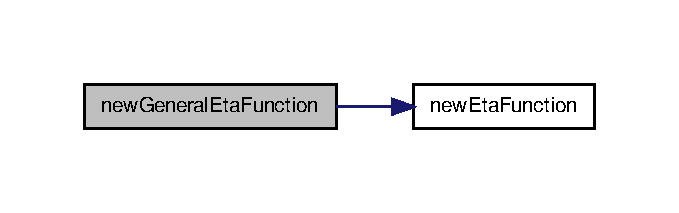
\includegraphics[width=326pt]{common_2measurement_8c_a018a3a7d15c126cbf15d03ba2698fe39_cgraph}
\end{center}
\end{figure}


\hypertarget{common_2measurement_8c_a25fcd9b89607eaa3abe03aea6ffe0447}{\index{common/measurement.\-c@{common/measurement.\-c}!new\-Log\-Cache@{new\-Log\-Cache}}
\index{new\-Log\-Cache@{new\-Log\-Cache}!common/measurement.c@{common/measurement.\-c}}
\subsubsection[{new\-Log\-Cache}]{\setlength{\rightskip}{0pt plus 5cm}{\bf \-Log\-Cache} {\bf new\-Log\-Cache} (
\begin{DoxyParamCaption}
\item[{size\-\_\-t}]{constants}
\end{DoxyParamCaption}
)}}\label{common_2measurement_8c_a25fcd9b89607eaa3abe03aea6ffe0447}


creates a new cache for logs of constants 


\begin{DoxyParams}{\-Parameters}
{\em constants} & number of constants \\
\hline
\end{DoxyParams}
\begin{DoxyReturn}{\-Returns}
new \-Log\-Cache 
\end{DoxyReturn}


\-Definition at line 203 of file measurement.\-c.



\-References s\-Log\-Cache\-::constants, s\-Log\-Cache\-::log\-C, and s\-Log\-Cache\-::log\-Not\-C.



\-Referenced by main().


\begin{DoxyCode}
{
    LogCache l;

    l = malloc(sizeof(struct sLogCache));

    l->constants = constants;

    l->logC = calloc(constants, sizeof(LogProbability));
    l->logNotC = calloc(constants, sizeof(LogProbability));

    return l;
}
\end{DoxyCode}
\hypertarget{common_2measurement_8c_a48c795067056a496c8e4aa903fac7d71}{\index{common/measurement.\-c@{common/measurement.\-c}!new\-Uniform\-Eta\-Function@{new\-Uniform\-Eta\-Function}}
\index{new\-Uniform\-Eta\-Function@{new\-Uniform\-Eta\-Function}!common/measurement.c@{common/measurement.\-c}}
\subsubsection[{new\-Uniform\-Eta\-Function}]{\setlength{\rightskip}{0pt plus 5cm}{\bf \-Eta\-Function} {\bf new\-Uniform\-Eta\-Function} (
\begin{DoxyParamCaption}
\item[{size\-\_\-t}]{types, }
\item[{size\-\_\-t}]{measurements}
\end{DoxyParamCaption}
)}}\label{common_2measurement_8c_a48c795067056a496c8e4aa903fac7d71}


create a new \-Eta\-Function with the same constant for each type 


\begin{DoxyParams}{\-Parameters}
{\em types} & \\
\hline
{\em measurements} & \\
\hline
\end{DoxyParams}
\begin{DoxyReturn}{\-Returns}

\end{DoxyReturn}


\-Definition at line 81 of file measurement.\-c.



\-References s\-Eta\-Function\-::eta, and new\-Eta\-Function().



\-Referenced by main().


\begin{DoxyCode}
{
    EtaFunction e;
    e = newEtaFunction(types, measurements, types);

    for (size_t t = 0; t < types; ++t)
    {
        for (size_t m = 0; m < measurements; ++m)
        {
            e->eta[t * measurements + m] = t;
        }
    }

    return e;
}
\end{DoxyCode}


\-Here is the call graph for this function\-:\nopagebreak
\begin{figure}[H]
\begin{center}
\leavevmode
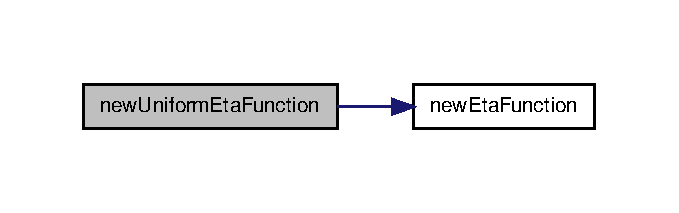
\includegraphics[width=326pt]{common_2measurement_8c_a48c795067056a496c8e4aa903fac7d71_cgraph}
\end{center}
\end{figure}


\hypertarget{common_2measurement_8c_a6441c79f9d24d9b47cf21dc69ab7638b}{\index{common/measurement.\-c@{common/measurement.\-c}!normalize\-Distance\-Matrix@{normalize\-Distance\-Matrix}}
\index{normalize\-Distance\-Matrix@{normalize\-Distance\-Matrix}!common/measurement.c@{common/measurement.\-c}}
\subsubsection[{normalize\-Distance\-Matrix}]{\setlength{\rightskip}{0pt plus 5cm}void {\bf normalize\-Distance\-Matrix} (
\begin{DoxyParamCaption}
\item[{{\bf \-Distance\-Matrix} restrict}]{d}
\end{DoxyParamCaption}
)}}\label{common_2measurement_8c_a6441c79f9d24d9b47cf21dc69ab7638b}


normalizes the distance matrix by replacing d with d', which is defined to be 

\[ d'(x,y) = d(x,y) - d(y,y) \]


\begin{DoxyParams}{\-Parameters}
{\em d} & distance matrix \\
\hline
\end{DoxyParams}


\-Definition at line 425 of file measurement.\-c.



\-References \-R\-E\-T\-U\-R\-N\-\_\-\-I\-F\-\_\-\-Z\-E\-R\-O.



\-Referenced by main().


\begin{DoxyCode}
{
    RETURN_IF_ZERO(d);

    for (size_t y = 0; y < d->objects; ++y)
    {
        LogProbability dyy;
        dyy = d->d[y*d->objects + y];

        for (size_t x = 0; x < d->objects; ++x)
        {
            /*
             * d(x,y) <- d(x,y) - d(y,y)
             */
            d->d[x*d->objects + y] -= dyy;
        }
    }
}
\end{DoxyCode}
\hypertarget{common_2measurement_8c_a6ec39ef8a7180bc340afed87c57ca604}{\index{common/measurement.\-c@{common/measurement.\-c}!sum\-Up@{sum\-Up}}
\index{sum\-Up@{sum\-Up}!common/measurement.c@{common/measurement.\-c}}
\subsubsection[{sum\-Up}]{\setlength{\rightskip}{0pt plus 5cm}{\bf \-Log\-Probability} {\bf sum\-Up} (
\begin{DoxyParamCaption}
\item[{const {\bf \-Log\-Probability} $\ast$restrict}]{\-V, }
\item[{size\-\_\-t}]{length, }
\item[{{\bf \-Log\-Probability}}]{lower\-\_\-bound, }
\item[{{\bf \-Log\-Probability}}]{upper\-\_\-bound}
\end{DoxyParamCaption}
)}}\label{common_2measurement_8c_a6ec39ef8a7180bc340afed87c57ca604}


\-This routine calculates the sum of elements of a vector. 


\begin{DoxyParams}{\-Parameters}
{\em \-V} & ptr to array of \-Log\-Probabilities \\
\hline
{\em length} & length of array \-V \\
\hline
{\em lower\-\_\-bound} & lower bound to include in this sum \\
\hline
{\em upper\-\_\-bound} & upper bound to include in this sum \\
\hline
\end{DoxyParams}
\begin{DoxyReturn}{\-Returns}
\[ \sum_{i=0, \mathrm{lower\_bound}\leq V(i) < \mathrm{upper\_bound}}^{ \mathrm{length}} V(i) \] 
\end{DoxyReturn}


\-Definition at line 305 of file measurement.\-c.



\-Referenced by log\-Probability\-From\-Product().


\begin{DoxyCode}
{
    //TODO: Make this routine smarter with respect to LARGE sums

    LogProbability sum;
    sum = 0.;

    for (size_t i = 0; i < length; ++i)
    {
        LogProbability summand;
        summand = V[i];

        if ((lower_bound <= summand) && (summand < upper_bound))
        {
            //printf("+%.2f",summand);
            sum += summand;
        }
    }
    //printf("=");

    return sum;
}
\end{DoxyCode}
\hypertarget{common_2measurement_8c_ad54d95f7de71efa2ad16ce6b133cf439}{\index{common/measurement.\-c@{common/measurement.\-c}!write\-Distances\-To\-File@{write\-Distances\-To\-File}}
\index{write\-Distances\-To\-File@{write\-Distances\-To\-File}!common/measurement.c@{common/measurement.\-c}}
\subsubsection[{write\-Distances\-To\-File}]{\setlength{\rightskip}{0pt plus 5cm}void {\bf write\-Distances\-To\-File} (
\begin{DoxyParamCaption}
\item[{const {\bf \-Distance\-Matrix}}]{d, }
\item[{const char $\ast$}]{filename}
\end{DoxyParamCaption}
)}}\label{common_2measurement_8c_ad54d95f7de71efa2ad16ce6b133cf439}


\-Writes the contents of a distance matrix to the given file in \-C\-S\-V format\-: d(x,y) will be written on the (x+1)th line to the (y+1)th column. 


\begin{DoxyParams}{\-Parameters}
{\em d} & the distance matrix \\
\hline
{\em filename} & output file name \\
\hline
\end{DoxyParams}


\-Definition at line 375 of file measurement.\-c.



\-References s\-Distance\-Matrix\-::d, s\-Distance\-Matrix\-::objects, and \-R\-E\-T\-U\-R\-N\-\_\-\-I\-F\-\_\-\-Z\-E\-R\-O.



\-Referenced by main().


\begin{DoxyCode}
{
    RETURN_IF_ZERO(d);
    RETURN_IF_ZERO(filename);

    FILE* file;
    file = fopen(filename, "w");

    RETURN_IF_ZERO(file);

    /*
     * header row
     */

    fputs("\"d(x,y)\"", file);

    for (size_t y = 0; y < d->objects; ++y)
    {
        fprintf(file, ",y=%zu", y);
    }

    fputs("\n", file);

    /*
     * contents
     */

    for (size_t x = 0; x < d->objects; ++x)
    {
        fprintf(file, "x=%zu", x);

        for (size_t y = 0; y < d->objects; ++y)
        {
            fprintf(file, ",%f", d->d[x * d->objects + y]);
        }

        fputs("\n", file);
    }

    fclose(file);
}
\end{DoxyCode}

\hypertarget{easy_2measurement_8c}{\section{src/fca/easy/measurement.c \-File \-Reference}
\label{easy_2measurement_8c}\index{src/fca/easy/measurement.\-c@{src/fca/easy/measurement.\-c}}
}
{\ttfamily \#include $<$string.\-h$>$}\*
{\ttfamily \#include $<$stdlib.\-h$>$}\*
{\ttfamily \#include $<$math.\-h$>$}\*
{\ttfamily \#include \char`\"{}private.\-h\char`\"{}}\*
\-Include dependency graph for measurement.\-c\-:\nopagebreak
\begin{figure}[H]
\begin{center}
\leavevmode
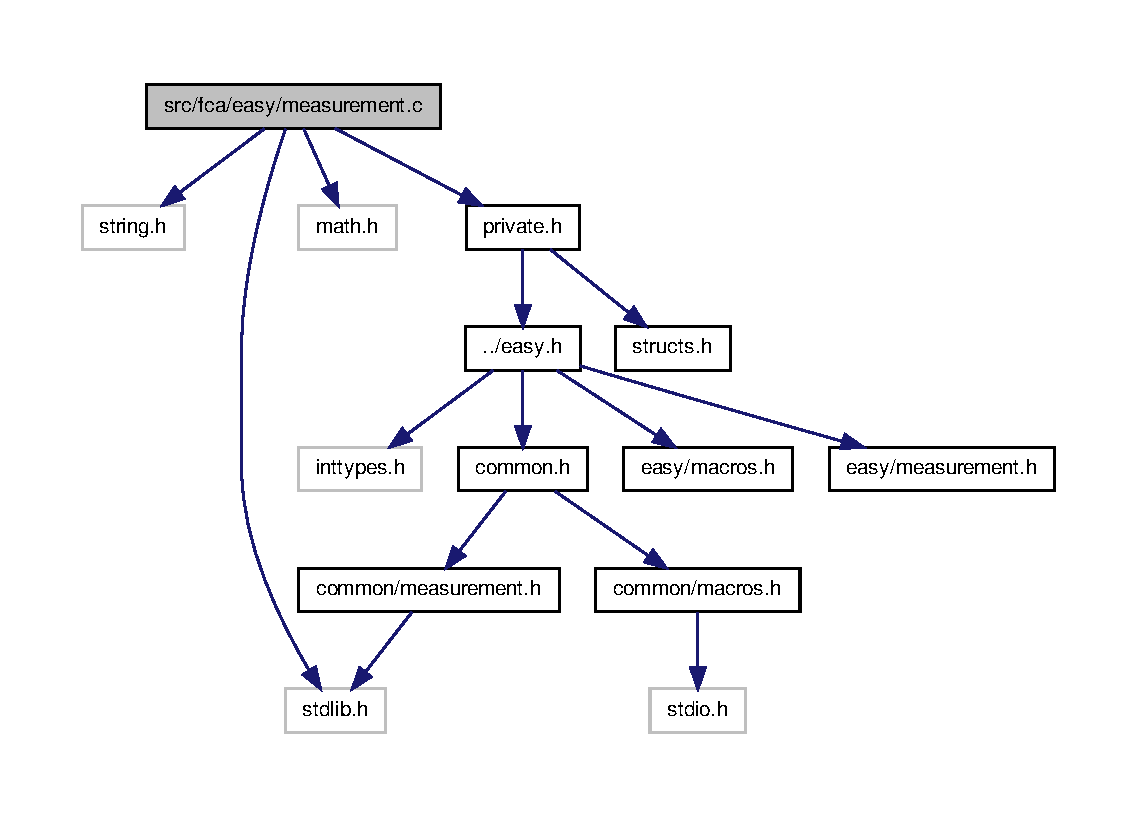
\includegraphics[width=350pt]{easy_2measurement_8c__incl}
\end{center}
\end{figure}
\subsection*{\-Functions}
\begin{DoxyCompactItemize}
\item 
void \hyperlink{easy_2measurement_8c_a0d243c594867f254694b0a91409d9b87}{calculate\-Likelihood} (const \hyperlink{easy_8h_ad53dc3fc96151a44387245e6481f95a4}{\-Formal\-Context} \-B, const \hyperlink{common_2measurement_8h_ab2f71cb9d9b10edcc10d44f79ee40d10}{\-Condition\-Map} c, const \hyperlink{easy_8h_ad53dc3fc96151a44387245e6481f95a4}{\-Formal\-Context} \-I, const \hyperlink{common_2measurement_8h_ab2406aaef0ce3e9f38a79f42ce470ffb}{\-Eta\-Function} eta, \hyperlink{common_2measurement_8h_afb8ffb8c068ef8c9fa3677762ac85994}{\-Commutative\-Product} \-L)
\begin{DoxyCompactList}\small\item\em measurement.\-c, (c) 2013, \-Immanuel \-Albrecht; \-Dresden \-University of \-Technology, \-Professur für die \-Psychologie des \-Lernen und \-Lehrens \end{DoxyCompactList}\item 
\hyperlink{easy_8h_ad53dc3fc96151a44387245e6481f95a4}{\-Formal\-Context} \hyperlink{easy_2measurement_8c_a9f03ccc14548b541ae120c6b869c1210}{new\-Fake\-Measurement} (const \hyperlink{easy_8h_ad53dc3fc96151a44387245e6481f95a4}{\-Formal\-Context} \-I, const \hyperlink{common_2measurement_8h_ab2406aaef0ce3e9f38a79f42ce470ffb}{\-Eta\-Function} eta, int experiments, \hyperlink{common_2measurement_8h_ab2f71cb9d9b10edcc10d44f79ee40d10}{\-Condition\-Map} $\ast$output\-\_\-c)
\begin{DoxyCompactList}\small\item\em generates a new formal context that comprises of a pseudo-\/random fake measurement obtained from \-I with the given error probabilites and experiment count \end{DoxyCompactList}\item 
void \hyperlink{easy_2measurement_8c_a521fc75fe217d457d76687a8cea85092}{optimize\-Condition\-Map} (const \hyperlink{easy_8h_ad53dc3fc96151a44387245e6481f95a4}{\-Formal\-Context} \-B, \hyperlink{common_2measurement_8h_ab2f71cb9d9b10edcc10d44f79ee40d10}{\-Condition\-Map} c, const \hyperlink{easy_8h_ad53dc3fc96151a44387245e6481f95a4}{\-Formal\-Context} \-I, const \hyperlink{common_2measurement_8h_ab2406aaef0ce3e9f38a79f42ce470ffb}{\-Eta\-Function} restrict eta, const \hyperlink{common_2measurement_8h_ace94e4c4dddc7766492a0f041a72963b}{\-Log\-Cache} log\-\_\-c)
\begin{DoxyCompactList}\small\item\em recalculate the condition map \-C, such that the likelihood of (\-B,c,\-I,eta) is maximal \end{DoxyCompactList}\item 
void \hyperlink{easy_2measurement_8c_a1de1f8bcc4d06953f1b5bb130389aa3f}{optimize\-Approximation\-Context} (const \hyperlink{easy_8h_ad53dc3fc96151a44387245e6481f95a4}{\-Formal\-Context} \-B, const \hyperlink{common_2measurement_8h_ab2f71cb9d9b10edcc10d44f79ee40d10}{\-Condition\-Map} cmap, \hyperlink{easy_8h_ad53dc3fc96151a44387245e6481f95a4}{\-Formal\-Context} \-I, const \hyperlink{common_2measurement_8h_ab2406aaef0ce3e9f38a79f42ce470ffb}{\-Eta\-Function} restrict eta, const \hyperlink{common_2measurement_8h_ace94e4c4dddc7766492a0f041a72963b}{\-Log\-Cache} log\-\_\-c)
\begin{DoxyCompactList}\small\item\em optimize the approximated context for a given measurement and condition map \end{DoxyCompactList}\item 
\hyperlink{common_2measurement_8h_a315318def4482768da7077f76ff0c768}{\-Distance\-Matrix} \hyperlink{easy_2measurement_8c_a63b673e042e8f51a7587322bf49ab7f2}{new\-Distance\-Matrix\-From\-Context} (const \hyperlink{easy_8h_ad53dc3fc96151a44387245e6481f95a4}{\-Formal\-Context} \-B, const \hyperlink{common_2measurement_8h_ab2406aaef0ce3e9f38a79f42ce470ffb}{\-Eta\-Function} restrict eta, const \hyperlink{common_2measurement_8h_ace94e4c4dddc7766492a0f041a72963b}{\-Log\-Cache} log\-\_\-c)
\begin{DoxyCompactList}\small\item\em calculates the asymmetric distances for some measurement context \end{DoxyCompactList}\end{DoxyCompactItemize}


\subsection{\-Function \-Documentation}
\hypertarget{easy_2measurement_8c_a0d243c594867f254694b0a91409d9b87}{\index{easy/measurement.\-c@{easy/measurement.\-c}!calculate\-Likelihood@{calculate\-Likelihood}}
\index{calculate\-Likelihood@{calculate\-Likelihood}!easy/measurement.c@{easy/measurement.\-c}}
\subsubsection[{calculate\-Likelihood}]{\setlength{\rightskip}{0pt plus 5cm}void {\bf calculate\-Likelihood} (
\begin{DoxyParamCaption}
\item[{const {\bf \-Formal\-Context}}]{\-B, }
\item[{const {\bf \-Condition\-Map}}]{c, }
\item[{const {\bf \-Formal\-Context}}]{\-I, }
\item[{const {\bf \-Eta\-Function}}]{eta, }
\item[{{\bf \-Commutative\-Product}}]{\-L}
\end{DoxyParamCaption}
)}}\label{easy_2measurement_8c_a0d243c594867f254694b0a91409d9b87}


measurement.\-c, (c) 2013, \-Immanuel \-Albrecht; \-Dresden \-University of \-Technology, \-Professur für die \-Psychologie des \-Lernen und \-Lehrens 

\hyperlink{easy_2measurement_8h}{easy/measurement.\-h}, (c) 2013, \-Immanuel \-Albrecht; \-Dresden \-University of \-Technology, \-Professur für die \-Psychologie des \-Lernen und \-Lehrens

\-This program is free software\-: you can redistribute it and/or modify it under the terms of the \-G\-N\-U \-General \-Public \-License as published by the \-Free \-Software \-Foundation, either version 3 of the \-License, or (at your option) any later version.

\-This program is distributed in the hope that it will be useful, but \-W\-I\-T\-H\-O\-U\-T \-A\-N\-Y \-W\-A\-R\-R\-A\-N\-T\-Y; without even the implied warranty of \-M\-E\-R\-C\-H\-A\-N\-T\-A\-B\-I\-L\-I\-T\-Y or \-F\-I\-T\-N\-E\-S\-S \-F\-O\-R \-A \-P\-A\-R\-T\-I\-C\-U\-L\-A\-R \-P\-U\-R\-P\-O\-S\-E. \-See the \-G\-N\-U \-General \-Public \-License for more details.

\-You should have received a copy of the \-G\-N\-U \-General \-Public \-License along with this program. \-If not, see $<$\href{http://www.gnu.org/licenses/}{\tt http\-://www.\-gnu.\-org/licenses/}$>$. calculates the likelihood function \-L 
\begin{DoxyParams}{\-Parameters}
{\em \-B} & the measurement context \\
\hline
{\em c} & the condition map (mapping objects \\
\hline
{\em \-I} & \\
\hline
{\em eta} & \\
\hline
{\em \-L} & \\
\hline
\end{DoxyParams}


\-Definition at line 34 of file measurement.\-c.



\-References s\-Condition\-Map\-::c, s\-Eta\-Function\-::constants, s\-Commutative\-Product\-::constants, s\-Eta\-Function\-::eta, g\-Im, s\-Commutative\-Product\-::match, s\-Eta\-Function\-::measurements, s\-Commutative\-Product\-::mismatch, s\-Condition\-Map\-::objects, \-R\-E\-T\-U\-R\-N\-\_\-\-I\-F\-\_\-\-Z\-E\-R\-O, s\-Eta\-Function\-::types, \-W\-A\-R\-N\-\_\-\-I\-F\-\_\-\-G\-E\-Q\-\_\-\-D\-O, and \-W\-A\-R\-N\-\_\-\-I\-F\-\_\-\-U\-N\-E\-Q\-U\-A\-L\-\_\-\-D\-O.


\begin{DoxyCode}
{
    RETURN_IF_ZERO(B);
    RETURN_IF_ZERO(c);
    RETURN_IF_ZERO(I);
    RETURN_IF_ZERO(eta);
    RETURN_IF_ZERO(L);

    const myFormalContext* restrict b;
    b = (const myFormalContext*) B;

    const myFormalContext* restrict i;
    i = (const myFormalContext*) I;

    WARN_IF_UNEQUAL_DO(b->objects, (int )c->objects, return);
    WARN_IF_UNEQUAL_DO(b->attributes, i->attributes, return);
    WARN_IF_UNEQUAL_DO(i->attributes, (int ) eta->measurements, return);
    WARN_IF_UNEQUAL_DO(2, eta->types, return);
    WARN_IF_UNEQUAL_DO(eta->constants, L->constants,);

    memset(L->match, 0, sizeof(size_t) * L->constants);
    memset(L->mismatch, 0, sizeof(size_t) * L->constants);

    for (int g = 0; g < b->objects; ++g)
    {
        int c_g;
        c_g = (int) c->c[g];

        WARN_IF_GEQ_DO(c_g, i->objects, continue);

        for (int m = 0; m < b->attributes; ++m)
        {
            if (gIm(c_g,i,m))
            {
                if (gIm(g,b,m))
                {
                    L->match[eta->eta[b->attributes + m]]++;
                }
                else
                {
                    L->mismatch[eta->eta[b->attributes + m]]++;
                }
            }
            else
            {
                if (gIm(g,b,m))
                {
                    L->mismatch[eta->eta[m]]++;
                }
                else
                {
                    L->match[eta->eta[m]]++;
                }
            }
        }
    }
}
\end{DoxyCode}
\hypertarget{easy_2measurement_8c_a63b673e042e8f51a7587322bf49ab7f2}{\index{easy/measurement.\-c@{easy/measurement.\-c}!new\-Distance\-Matrix\-From\-Context@{new\-Distance\-Matrix\-From\-Context}}
\index{new\-Distance\-Matrix\-From\-Context@{new\-Distance\-Matrix\-From\-Context}!easy/measurement.c@{easy/measurement.\-c}}
\subsubsection[{new\-Distance\-Matrix\-From\-Context}]{\setlength{\rightskip}{0pt plus 5cm}{\bf \-Distance\-Matrix} {\bf new\-Distance\-Matrix\-From\-Context} (
\begin{DoxyParamCaption}
\item[{const {\bf \-Formal\-Context}}]{\-B, }
\item[{const {\bf \-Eta\-Function} restrict}]{eta, }
\item[{const {\bf \-Log\-Cache}}]{log\-\_\-c}
\end{DoxyParamCaption}
)}}\label{easy_2measurement_8c_a63b673e042e8f51a7587322bf49ab7f2}


calculates the asymmetric distances for some measurement context 


\begin{DoxyParams}{\-Parameters}
{\em \-B} & the measurement context \\
\hline
{\em eta} & the error probabilities \\
\hline
{\em log\-\_\-c} & the logarithms corresponding to eta \\
\hline
\end{DoxyParams}
\begin{DoxyReturn}{\-Returns}
a new \-Distance\-Matrix 
\end{DoxyReturn}


\-Definition at line 469 of file measurement.\-c.



\-References s\-Log\-Cache\-::constants, delete\-Commutative\-Product(), g\-Im, log\-Probability\-From\-Product(), s\-Commutative\-Product\-::match, s\-Commutative\-Product\-::mismatch, new\-Commutative\-Product(), new\-Distance\-Matrix(), \-R\-E\-T\-U\-R\-N\-\_\-\-Z\-E\-R\-O\-\_\-\-I\-F\-\_\-\-Z\-E\-R\-O, and \-W\-A\-R\-N\-\_\-\-I\-F\-\_\-\-U\-N\-E\-Q\-U\-A\-L\-\_\-\-D\-O.



\-Referenced by main().


\begin{DoxyCode}
{
    RETURN_ZERO_IF_ZERO(B);
    RETURN_ZERO_IF_ZERO(eta);
    RETURN_ZERO_IF_ZERO(log_c);

    const myFormalContext* restrict b;
    b = (const myFormalContext*) B;

    WARN_IF_UNEQUAL_DO(b->attributes, (int )eta->measurements, return 0);
    WARN_IF_UNEQUAL_DO(2, eta->types, return 0);
    WARN_IF_UNEQUAL_DO(eta->constants, log_c->constants, return 0);

    size_t attributes;
    attributes = (size_t) b->attributes;

#pragma GCC diagnostic push
#pragma GCC diagnostic ignored "-Wsign-conversion"

    size_t measurements;
    measurements = b->objects;

#pragma GCC diagnostic pop

    DistanceMatrix d;
    d = newDistanceMatrix(measurements);

    CommutativeProduct dxy, dyx;

    dxy = newCommutativeProduct(eta->constants);
    dyx = newCommutativeProduct(eta->constants);

    /*
     * calculate the distances d(x,y) and d(y,x) in parallel
     */

    for (size_t x = 0; x < measurements; ++x)
    {
        for (size_t y = x; y < measurements; ++y)
        {
            /*
             * set dxy and dyx to zero
             */
            for (size_t i = 0; i < eta->constants; ++i)
            {
                dxy->match[i] = 0;
                dxy->mismatch[i] = 0;

                dyx->match[i] = 0;
                dyx->mismatch[i] = 0;
            }

            /*
             * check where the attribute vectors coincide and where not
             */

            for (size_t m = 0; m < attributes; ++m)
            {
                size_t eta_m0, eta_m1;

                eta_m0 = eta->eta[0 * eta->constants + m];
                eta_m1 = eta->eta[1 * eta->constants + m];

#pragma GCC diagnostic push
#pragma GCC diagnostic ignored "-Wsign-conversion"

                if (gIm(x,b,m))
                {
                    if (gIm(y,b,m))
                    {

                        dxy->match[eta_m1]++;
                        dyx->match[eta_m1]++;
                    }
                    else
                    {
                        dxy->mismatch[eta_m1]++;
                        dyx->mismatch[eta_m0]++;
                    }
                }
                else
                {
                    if (gIm(y,b,m))
                    {
                        dxy->mismatch[eta_m0]++;
                        dyx->mismatch[eta_m1]++;
                    }
                    else
                    {
                        dxy->match[eta_m0]++;
                        dyx->match[eta_m0]++;
                    }
                }

#pragma GCC diagnostic pop
            }

            /*
             * calculate the logarithms of the likelihoods
             */

            d->d[x * measurements + y] = logProbabilityFromProduct(log_c, dxy);
            d->d[y * measurements + x] = logProbabilityFromProduct(log_c, dyx);
        }
    }

    deleteCommutativeProduct(&dxy);
    deleteCommutativeProduct(&dyx);

    return d;
}
\end{DoxyCode}


\-Here is the call graph for this function\-:\nopagebreak
\begin{figure}[H]
\begin{center}
\leavevmode
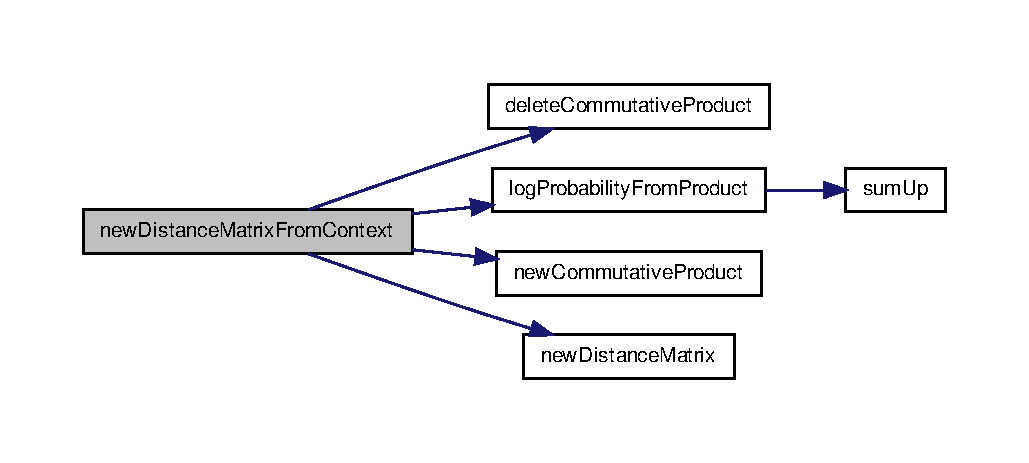
\includegraphics[width=350pt]{easy_2measurement_8c_a63b673e042e8f51a7587322bf49ab7f2_cgraph}
\end{center}
\end{figure}


\hypertarget{easy_2measurement_8c_a9f03ccc14548b541ae120c6b869c1210}{\index{easy/measurement.\-c@{easy/measurement.\-c}!new\-Fake\-Measurement@{new\-Fake\-Measurement}}
\index{new\-Fake\-Measurement@{new\-Fake\-Measurement}!easy/measurement.c@{easy/measurement.\-c}}
\subsubsection[{new\-Fake\-Measurement}]{\setlength{\rightskip}{0pt plus 5cm}{\bf \-Formal\-Context} {\bf new\-Fake\-Measurement} (
\begin{DoxyParamCaption}
\item[{const {\bf \-Formal\-Context}}]{\-I, }
\item[{const {\bf \-Eta\-Function}}]{eta, }
\item[{int}]{experiments, }
\item[{{\bf \-Condition\-Map} $\ast$}]{output\-\_\-c}
\end{DoxyParamCaption}
)}}\label{easy_2measurement_8c_a9f03ccc14548b541ae120c6b869c1210}


generates a new formal context that comprises of a pseudo-\/random fake measurement obtained from \-I with the given error probabilites and experiment count 


\begin{DoxyParams}{\-Parameters}
{\em \-I} & experimental condition context \\
\hline
{\em eta} & error probabilities \\
\hline
{\em experiments} & number of conducted experiments \\
\hline
{\em output\-\_\-c} & a new \-Condition\-Map will be generated to this pointer, if nonzero \\
\hline
\end{DoxyParams}
\begin{DoxyReturn}{\-Returns}
a new \-Formal\-Context object 
\end{DoxyReturn}


\-Definition at line 103 of file measurement.\-c.



\-References s\-Eta\-Function\-::\-C, \-C\-E\-L\-L, \-C\-R\-O\-S\-S, s\-Eta\-Function\-::eta, g\-Im, s\-Eta\-Function\-::measurements, \-M\-I\-N, new\-Condition\-Map(), new\-Formal\-Context, \-R\-E\-T\-U\-R\-N\-\_\-\-Z\-E\-R\-O\-\_\-\-I\-F\-\_\-\-Z\-E\-R\-O, and \-W\-A\-R\-N\-\_\-\-I\-F\-\_\-\-U\-N\-E\-Q\-U\-A\-L\-\_\-\-D\-O.



\-Referenced by main().


\begin{DoxyCode}
{
    RETURN_ZERO_IF_ZERO(I);
    RETURN_ZERO_IF_ZERO(eta);

    const myFormalContext* restrict i;
    i = (const myFormalContext*) I;

    WARN_IF_UNEQUAL_DO(i->attributes, (int ) eta->measurements, return 0);

#pragma GCC diagnostic push
#pragma GCC diagnostic ignored "-Wsign-conversion"

    if (output_c)
        *output_c = newConditionMap(experiments);

#pragma GCC diagnostic pop

    myFormalContext *b;
    b = (myFormalContext *) newFormalContext(experiments, i->attributes);

    for (int x = 0; x < experiments; ++x)
    {
        int c_x;
        c_x =
                MIN((int) floor((double) (random()) /
                                (double) RAND_MAX * (double)i->objects), i->
      objects-1);

#pragma GCC diagnostic push
#pragma GCC diagnostic ignored "-Wsign-conversion"

        if (output_c)
            (*output_c)->c[x] = c_x;

#pragma GCC diagnostic pop

        for (int m = 0; m < i->attributes; ++m)
        {
            Probability rnd;
            rnd = (Probability) random() / (Probability) RAND_MAX;

            if (gIm(c_x,i,m))
            {
                if (rnd >= eta->C[eta->eta[i->attributes + m]])
                    CROSS(CELL(x,b,m));
            }
            else
            {
                if (rnd < eta->C[eta->eta[m]])
                    CROSS(CELL(x,b,m));
            }
        }
    }

    return (FormalContext) b;
}
\end{DoxyCode}


\-Here is the call graph for this function\-:\nopagebreak
\begin{figure}[H]
\begin{center}
\leavevmode
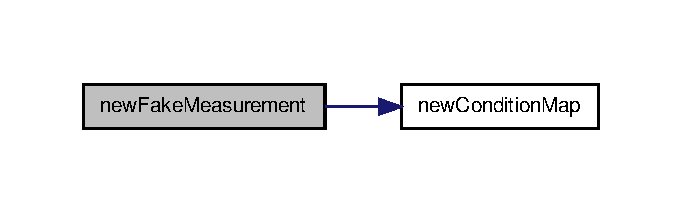
\includegraphics[width=328pt]{easy_2measurement_8c_a9f03ccc14548b541ae120c6b869c1210_cgraph}
\end{center}
\end{figure}


\hypertarget{easy_2measurement_8c_a1de1f8bcc4d06953f1b5bb130389aa3f}{\index{easy/measurement.\-c@{easy/measurement.\-c}!optimize\-Approximation\-Context@{optimize\-Approximation\-Context}}
\index{optimize\-Approximation\-Context@{optimize\-Approximation\-Context}!easy/measurement.c@{easy/measurement.\-c}}
\subsubsection[{optimize\-Approximation\-Context}]{\setlength{\rightskip}{0pt plus 5cm}void {\bf optimize\-Approximation\-Context} (
\begin{DoxyParamCaption}
\item[{const {\bf \-Formal\-Context}}]{\-B, }
\item[{const {\bf \-Condition\-Map}}]{cmap, }
\item[{{\bf \-Formal\-Context}}]{\-I, }
\item[{const {\bf \-Eta\-Function} restrict}]{eta, }
\item[{const {\bf \-Log\-Cache}}]{log\-\_\-c}
\end{DoxyParamCaption}
)}}\label{easy_2measurement_8c_a1de1f8bcc4d06953f1b5bb130389aa3f}


optimize the approximated context for a given measurement and condition map 


\begin{DoxyParams}{\-Parameters}
{\em \-B} & the measurement context \\
\hline
{\em cmap} & condition map \\
\hline
{\em \-I} & output\-: new approximated context \\
\hline
{\em eta} & the error probabilities \\
\hline
{\em log\-\_\-c} & log constants corresponding to eta \\
\hline
\end{DoxyParams}


\-Definition at line 314 of file measurement.\-c.



\-References smy\-Formal\-Context\-::attributes, s\-Condition\-Map\-::c, \-C\-E\-L\-L, \-C\-L\-E\-A\-R, s\-Log\-Cache\-::constants, \-C\-R\-O\-S\-S, delete\-Commutative\-Product(), g\-Im, log\-Probability\-From\-Product(), new\-Commutative\-Product(), smy\-Formal\-Context\-::objects, s\-Condition\-Map\-::objects, \-R\-E\-T\-U\-R\-N\-\_\-\-I\-F\-\_\-\-Z\-E\-R\-O, and \-W\-A\-R\-N\-\_\-\-I\-F\-\_\-\-U\-N\-E\-Q\-U\-A\-L\-\_\-\-D\-O.



\-Referenced by main().


\begin{DoxyCode}
{
    RETURN_IF_ZERO(B);
    RETURN_IF_ZERO(cmap);
    RETURN_IF_ZERO(I);
    RETURN_IF_ZERO(eta);
    RETURN_IF_ZERO(log_c);

    const myFormalContext* restrict b;
    b = (const myFormalContext*) B;

    myFormalContext* i;
    i = (myFormalContext*) I;

    WARN_IF_UNEQUAL_DO(b->objects, (int )cmap->objects, return);
    WARN_IF_UNEQUAL_DO(b->attributes, i->attributes, return);
    WARN_IF_UNEQUAL_DO(b->attributes, (int )eta->measurements, return);
    WARN_IF_UNEQUAL_DO(2, eta->types, return);
    WARN_IF_UNEQUAL_DO(eta->constants, log_c->constants, return);

    size_t attributes;
    attributes = (size_t) b->attributes;

#pragma GCC diagnostic push
#pragma GCC diagnostic ignored "-Wsign-conversion"

    size_t measurements;
    measurements = b->objects;

    size_t conditions;
    conditions = i->objects;

#pragma GCC diagnostic pop

    CommutativeProduct *l_array;

    l_array = malloc(sizeof(CommutativeProduct) * conditions * 2);

    CommutativeProduct restrict * l_cross;
    l_cross = (CommutativeProduct restrict *) l_array;

    CommutativeProduct restrict * l_gap;
    l_gap = (CommutativeProduct restrict *) (l_array + conditions);

    for (size_t c = 0; c < conditions; ++c)
    {
        l_cross[c] = newCommutativeProduct(eta->constants);
        l_gap[c] = newCommutativeProduct(eta->constants);
    }

    /*
     * check column wise, whether there should be a cross in the incidence
       matrix I
     * or not.
     */

    for (size_t a = 0; a < attributes; ++a)
    {
        size_t eta_a0, eta_a1;

        eta_a0 = eta->eta[0 * eta->constants + a];
        eta_a1 = eta->eta[1 * eta->constants + a];

        for (size_t c = 0; c < conditions; ++c)
        {
            for (size_t i = 0; i < eta->constants; ++i)
            {
                l_cross[c]->match[i] = 0;
                l_cross[c]->mismatch[i] = 0;
                l_gap[c]->match[i] = 0;
                l_gap[c]->mismatch[i] = 0;
            }
        }

        /*
         * count how often we measured attribute a for each condition cmap
         * and fill it in the corresponding CommutativeProduct
         */

        for (size_t o = 0; o < measurements; ++o)
        {
            size_t condition;
            condition = cmap->c[o];

            /*
             * add up in parallel both error vectors for both cross and gap
       case
             * in the approximation
             */

#pragma GCC diagnostic push
#pragma GCC diagnostic ignored "-Wsign-conversion"

            if (gIm(o, b, a))
            {
                l_cross[condition]->match[eta_a1]++;
                l_gap[condition]->mismatch[eta_a0]++;
            }
            else
            {
                l_cross[condition]->mismatch[eta_a1]++;
                l_gap[condition]->match[eta_a0]++;
            }

#pragma GCC diagnostic pop
        }

        /*
         * now each l_cross[c] and l_gap[c] contain the same indexed factors
       for
         * the likelihoods with and without a cross for c I a
         * we sum up both and the bigger wins
         */

        for (size_t c = 0; c < conditions; ++c)
        {
            LogProbability cross;
            LogProbability gap;

            cross = logProbabilityFromProduct(log_c, l_cross[c]);
            gap = logProbabilityFromProduct(log_c, l_gap[c]);

#pragma GCC diagnostic push
#pragma GCC diagnostic ignored "-Wsign-conversion"

            if (gap <= cross)
            {
                CROSS(CELL(c,i,a));
            }
            else
            {
                CLEAR(CELL(c,i,a));
            }

#pragma GCC diagnostic pop
        }
    }

    for (size_t c = 0; c < conditions; ++c)
    {
        deleteCommutativeProduct(l_array + c);
        deleteCommutativeProduct(l_array + c + conditions);
    }

    free(l_array);
}
\end{DoxyCode}


\-Here is the call graph for this function\-:\nopagebreak
\begin{figure}[H]
\begin{center}
\leavevmode
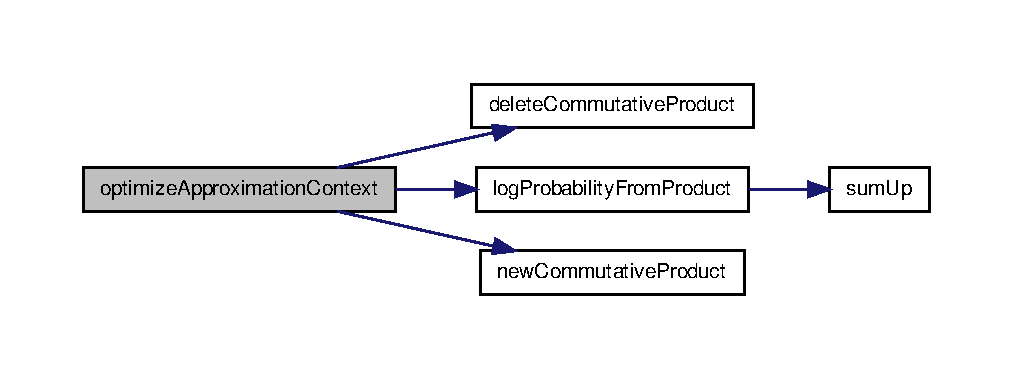
\includegraphics[width=350pt]{easy_2measurement_8c_a1de1f8bcc4d06953f1b5bb130389aa3f_cgraph}
\end{center}
\end{figure}


\hypertarget{easy_2measurement_8c_a521fc75fe217d457d76687a8cea85092}{\index{easy/measurement.\-c@{easy/measurement.\-c}!optimize\-Condition\-Map@{optimize\-Condition\-Map}}
\index{optimize\-Condition\-Map@{optimize\-Condition\-Map}!easy/measurement.c@{easy/measurement.\-c}}
\subsubsection[{optimize\-Condition\-Map}]{\setlength{\rightskip}{0pt plus 5cm}void {\bf optimize\-Condition\-Map} (
\begin{DoxyParamCaption}
\item[{const {\bf \-Formal\-Context}}]{\-B, }
\item[{{\bf \-Condition\-Map}}]{c, }
\item[{const {\bf \-Formal\-Context}}]{\-I, }
\item[{const {\bf \-Eta\-Function} restrict}]{eta, }
\item[{const {\bf \-Log\-Cache}}]{log\-\_\-c}
\end{DoxyParamCaption}
)}}\label{easy_2measurement_8c_a521fc75fe217d457d76687a8cea85092}


recalculate the condition map \-C, such that the likelihood of (\-B,c,\-I,eta) is maximal 


\begin{DoxyParams}{\-Parameters}
{\em \-B} & the measurement context \\
\hline
{\em c} & output\-: \-Condition\-Map that will be filled with c\-\_\-\{\-I,eta\} \\
\hline
{\em \-I} & the condition context \\
\hline
{\em eta} & the error probabilities \\
\hline
{\em log\-\_\-c} & log constants corresponding to eta \\
\hline
\end{DoxyParams}


\-Definition at line 171 of file measurement.\-c.



\-References s\-Condition\-Map\-::c, s\-Log\-Cache\-::constants, delete\-Commutative\-Product(), g\-Im, \-L\-O\-G\-\_\-\-P\-R\-O\-B\-\_\-\-L\-O\-W\-E\-R\-\_\-\-B\-O\-U\-N\-D, log\-Probability\-From\-Product(), new\-Commutative\-Product(), s\-Condition\-Map\-::objects, \-R\-E\-T\-U\-R\-N\-\_\-\-I\-F\-\_\-\-Z\-E\-R\-O, and \-W\-A\-R\-N\-\_\-\-I\-F\-\_\-\-U\-N\-E\-Q\-U\-A\-L\-\_\-\-D\-O.



\-Referenced by main().


\begin{DoxyCode}
{
    RETURN_IF_ZERO(B);
    RETURN_IF_ZERO(c);
    RETURN_IF_ZERO(I);
    RETURN_IF_ZERO(eta);
    RETURN_IF_ZERO(log_c);

    const myFormalContext* restrict b;
    b = (const myFormalContext*) B;

    const myFormalContext* restrict i;
    i = (const myFormalContext*) I;

    WARN_IF_UNEQUAL_DO(b->objects, (int )c->objects, return);
    WARN_IF_UNEQUAL_DO(b->attributes, i->attributes, return);
    WARN_IF_UNEQUAL_DO(b->attributes, (int )eta->measurements, return);
    WARN_IF_UNEQUAL_DO(2, eta->types, return);
    WARN_IF_UNEQUAL_DO(eta->constants, log_c->constants, return);

    size_t attributes;
    attributes = (size_t) b->attributes;

    CommutativeProduct lp;
    lp = newCommutativeProduct(eta->constants);

    CommutativeProduct restrict l;
    l = lp;

    /*
     * For every object index x of B, find the last object index of I, such
       that
     * the likelihood that experiment x was conducted under that condition is
       maximal.
     */

    for (size_t x = 0; x < (size_t) b->objects; ++x)
    {

        size_t best_cx;
        best_cx = 0;

        /*
         * initialize the current maximal probability with the bottom value of
         * LogProbability
         */

        LogProbability maximal_prob;
        maximal_prob = LOG_PROB_LOWER_BOUND;

        for (size_t cx = 0; cx < (size_t) i->objects; ++cx)
        {
            /*
             * calculate (partial) likelihood if c(x) = cx
             */
            memset(l->match, 0, sizeof(size_t) * l->constants);
            memset(l->mismatch, 0, sizeof(size_t) * l->constants);

            for (size_t m = 0; m < attributes; ++m)
            {
#pragma GCC diagnostic push
#pragma GCC diagnostic ignored "-Wsign-conversion"
                if (gIm(x,b,m))
                {
                    if (gIm(cx,i,m))
                    {
#pragma GCC diagnostic pop
                        /*
                         * 1-eta(m,1)
                         */
                        l->match[eta->eta[1 * eta->constants + m]]++;
                        //printf("X");
                    }
                    else
                    {
                        /*
                         * eta(m,0)
                         */
                        l->mismatch[eta->eta[0 * eta->constants + m]]++;
                        //printf("O");
                    }
                }
                else
                {
#pragma GCC diagnostic push
#pragma GCC diagnostic ignored "-Wsign-conversion"
                    if (gIm(cx,i,m))
                    {
#pragma GCC diagnostic pop
                        /*
                         * eta(m,1)
                         */
                        l->mismatch[eta->eta[1 * eta->constants + m]]++;
                        //printf("_");
                    }
                    else
                    {
                        /*
                         * 1-eta(m,0)
                         */
                        l->match[eta->eta[0 * eta->constants + m]]++;
                        //printf(".");
                    }
                }
            }

            LogProbability p;
            p = logProbabilityFromProduct(log_c, l);

            //printf("%f\t", p);

            /*
             * cx is more likely than best_cx
             * so, update cx -> best_cx
             */

            if (maximal_prob <= p)
            {
                maximal_prob = p;
                best_cx = cx;
            }
        }

        /*
         * choose the most likely match
         */

        c->c[x] = best_cx;
        //printf("c(%4zu) = %4zu\n", x, c->c[x]);
    }

    deleteCommutativeProduct(&lp);
}
\end{DoxyCode}


\-Here is the call graph for this function\-:\nopagebreak
\begin{figure}[H]
\begin{center}
\leavevmode
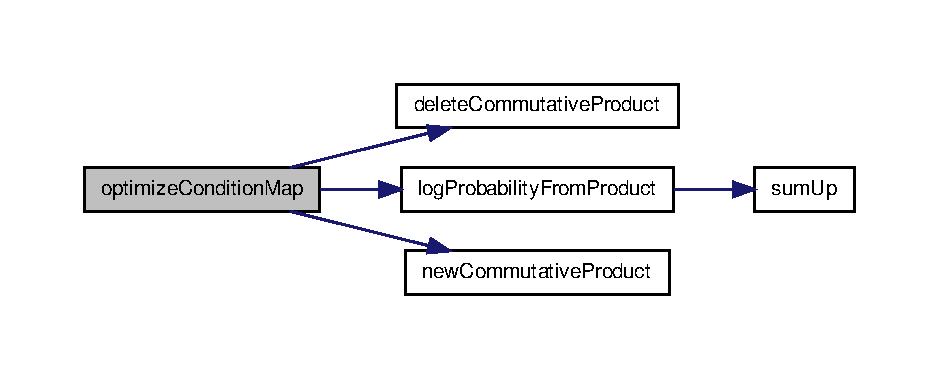
\includegraphics[width=350pt]{easy_2measurement_8c_a521fc75fe217d457d76687a8cea85092_cgraph}
\end{center}
\end{figure}



\hypertarget{common_2measurement_8h}{\section{src/fca/common/measurement.h \-File \-Reference}
\label{common_2measurement_8h}\index{src/fca/common/measurement.\-h@{src/fca/common/measurement.\-h}}
}
{\ttfamily \#include $<$stdlib.\-h$>$}\*
{\ttfamily \#include $<$float.\-h$>$}\*
\-Include dependency graph for measurement.\-h\-:\nopagebreak
\begin{figure}[H]
\begin{center}
\leavevmode
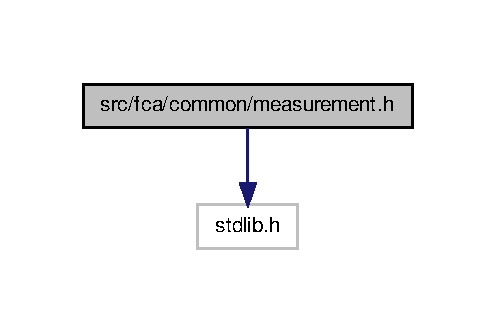
\includegraphics[width=238pt]{common_2measurement_8h__incl}
\end{center}
\end{figure}
\-This graph shows which files directly or indirectly include this file\-:\nopagebreak
\begin{figure}[H]
\begin{center}
\leavevmode
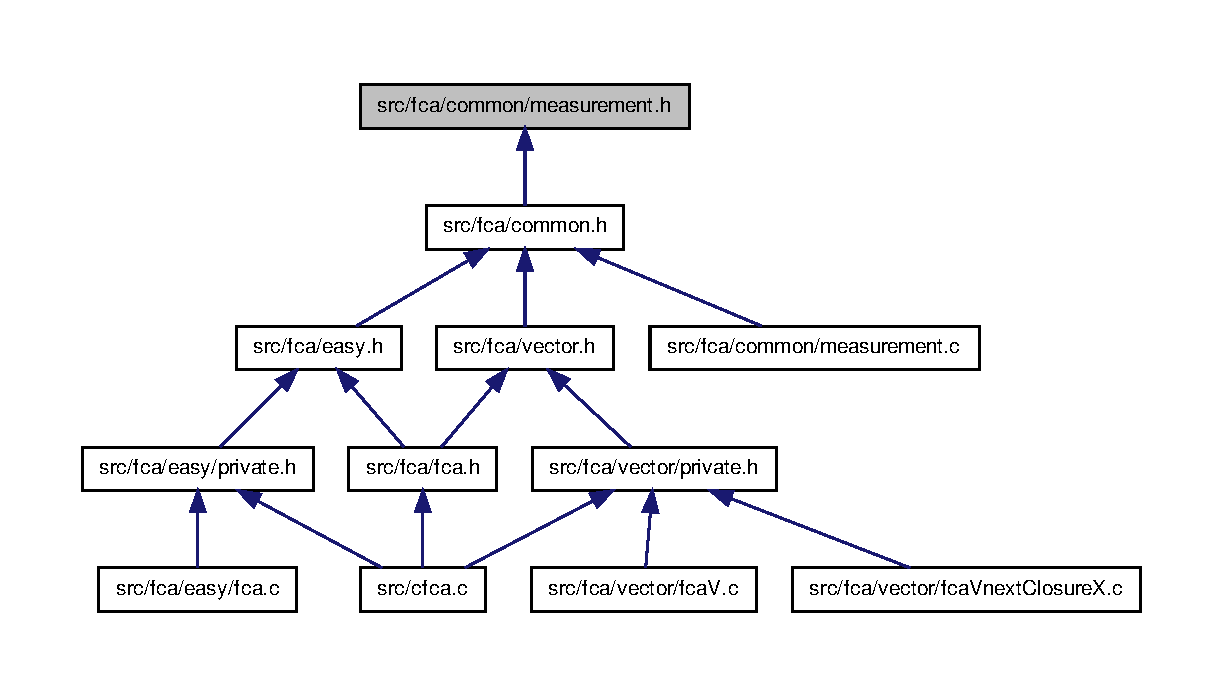
\includegraphics[width=350pt]{common_2measurement_8h__dep__incl}
\end{center}
\end{figure}
\subsection*{\-Data \-Structures}
\begin{DoxyCompactItemize}
\item 
struct \hyperlink{structsEtaFunction}{s\-Eta\-Function}
\begin{DoxyCompactList}\small\item\em this structure contains information on how many cases for measurements there are, and what the probabilities of erroneous measurement there is for each case \end{DoxyCompactList}\item 
struct \hyperlink{structsCommutativeProduct}{s\-Commutative\-Product}
\begin{DoxyCompactList}\small\item\em \-This struct represents a formal product of formal constants x\-\_\-i and their counterparts (1-\/x\-\_\-i) under the assumption of communtativity of the product. \end{DoxyCompactList}\item 
struct \hyperlink{structsConditionMap}{s\-Condition\-Map}
\begin{DoxyCompactList}\small\item\em \-This struct represents a map between the object sets of two formal contexts. \end{DoxyCompactList}\item 
struct \hyperlink{structsLogCache}{s\-Log\-Cache}
\begin{DoxyCompactList}\small\item\em \-This structure stores the logarithms of probabilities and of their complements. \end{DoxyCompactList}\end{DoxyCompactItemize}
\subsection*{\-Defines}
\begin{DoxyCompactItemize}
\item 
\#define \hyperlink{common_2measurement_8h_a0b858a576d6a3db1ea8020021d49896c}{\-L\-O\-G\-\_\-\-P\-R\-O\-B\-\_\-\-L\-O\-W\-E\-R\-\_\-\-B\-O\-U\-N\-D}~(-\/\-D\-B\-L\-\_\-\-M\-A\-X)
\item 
\#define \hyperlink{common_2measurement_8h_a34f2d788868c9760922910e9444443a1}{\-L\-O\-G\-\_\-\-P\-R\-O\-B\-\_\-\-U\-P\-P\-E\-R\-\_\-\-B\-O\-U\-N\-D}~(1.)
\end{DoxyCompactItemize}
\subsection*{\-Typedefs}
\begin{DoxyCompactItemize}
\item 
typedef double \hyperlink{common_2measurement_8h_ae6d7a8c80f18bc080ab1cfa38d119724}{\-Probability}
\begin{DoxyCompactList}\small\item\em measurement.\-h, (c) 2013, \-Immanuel \-Albrecht; \-Dresden \-University of \-Technology, \-Professur für die \-Psychologie des \-Lernen und \-Lehrens \end{DoxyCompactList}\item 
typedef double \hyperlink{common_2measurement_8h_a0a02860cc83aa9ce63d00855bc9058e0}{\-Log\-Probability}
\item 
typedef struct \hyperlink{structsEtaFunction}{s\-Eta\-Function} $\ast$ \hyperlink{common_2measurement_8h_ab2406aaef0ce3e9f38a79f42ce470ffb}{\-Eta\-Function}
\begin{DoxyCompactList}\small\item\em this structure contains information on how many cases for measurements there are, and what the probabilities of erroneous measurement there is for each case \end{DoxyCompactList}\item 
typedef struct \*
\hyperlink{structsCommutativeProduct}{s\-Commutative\-Product} $\ast$ \hyperlink{common_2measurement_8h_afb8ffb8c068ef8c9fa3677762ac85994}{\-Commutative\-Product}
\begin{DoxyCompactList}\small\item\em \-This struct represents a formal product of formal constants x\-\_\-i and their counterparts (1-\/x\-\_\-i) under the assumption of communtativity of the product. \end{DoxyCompactList}\item 
typedef struct \hyperlink{structsConditionMap}{s\-Condition\-Map} $\ast$ \hyperlink{common_2measurement_8h_ab2f71cb9d9b10edcc10d44f79ee40d10}{\-Condition\-Map}
\begin{DoxyCompactList}\small\item\em \-This struct represents a map between the object sets of two formal contexts. \end{DoxyCompactList}\item 
typedef struct \hyperlink{structsLogCache}{s\-Log\-Cache} $\ast$ \hyperlink{common_2measurement_8h_ace94e4c4dddc7766492a0f041a72963b}{\-Log\-Cache}
\begin{DoxyCompactList}\small\item\em \-This structure stores the logarithms of probabilities and of their complements. \end{DoxyCompactList}\end{DoxyCompactItemize}
\subsection*{\-Functions}
\begin{DoxyCompactItemize}
\item 
\hyperlink{common_2measurement_8h_ab2406aaef0ce3e9f38a79f42ce470ffb}{\-Eta\-Function} \hyperlink{common_2measurement_8h_aa0f12091b86c478e159761719923bd9a}{new\-Eta\-Function} (size\-\_\-t types, size\-\_\-t measurements, size\-\_\-t constants)
\begin{DoxyCompactList}\small\item\em creates a new \-Eta\-Function \end{DoxyCompactList}\item 
\hyperlink{common_2measurement_8h_ab2406aaef0ce3e9f38a79f42ce470ffb}{\-Eta\-Function} \hyperlink{common_2measurement_8h_a48c795067056a496c8e4aa903fac7d71}{new\-Uniform\-Eta\-Function} (size\-\_\-t types, size\-\_\-t measurements)
\begin{DoxyCompactList}\small\item\em create a new \-Eta\-Function with the same constant for each type \end{DoxyCompactList}\item 
\hyperlink{common_2measurement_8h_ab2406aaef0ce3e9f38a79f42ce470ffb}{\-Eta\-Function} \hyperlink{common_2measurement_8h_a018a3a7d15c126cbf15d03ba2698fe39}{new\-General\-Eta\-Function} (size\-\_\-t types, size\-\_\-t measurements)
\begin{DoxyCompactList}\small\item\em create a new \-Eta\-Function with the a constant for each type and measurement on its own \end{DoxyCompactList}\item 
void \hyperlink{common_2measurement_8h_a2905b59d4a364111890224a444fd6d30}{delete\-Eta\-Function} (\hyperlink{common_2measurement_8h_ab2406aaef0ce3e9f38a79f42ce470ffb}{\-Eta\-Function} $\ast$eta)
\begin{DoxyCompactList}\small\item\em deletes an \-Eta\-Function and sets the pointer to zero \end{DoxyCompactList}\item 
\hyperlink{common_2measurement_8h_afb8ffb8c068ef8c9fa3677762ac85994}{\-Commutative\-Product} \hyperlink{common_2measurement_8h_abe35a2e2ccf6060635d4daf6d6ebf59e}{new\-Commutative\-Product} (size\-\_\-t constants)
\begin{DoxyCompactList}\small\item\em creates a new commutative product without any factors \end{DoxyCompactList}\item 
void \hyperlink{common_2measurement_8h_a2120fbc047167fd0a08f3015b8716cd1}{delete\-Commutative\-Product} (\hyperlink{common_2measurement_8h_afb8ffb8c068ef8c9fa3677762ac85994}{\-Commutative\-Product} $\ast$p)
\begin{DoxyCompactList}\small\item\em deletes a \-Commutative\-Product and sets its pointer to zero. \end{DoxyCompactList}\item 
\hyperlink{common_2measurement_8h_ab2f71cb9d9b10edcc10d44f79ee40d10}{\-Condition\-Map} \hyperlink{common_2measurement_8h_ac4b7705e5a5c82b5d59b67617e6f2dc4}{new\-Condition\-Map} (size\-\_\-t objects)
\begin{DoxyCompactList}\small\item\em creates a new condition map \end{DoxyCompactList}\item 
void \hyperlink{common_2measurement_8h_ad40c601ad1dcd904cde0e9ebe2828d72}{delete\-Condition\-Map} (\hyperlink{common_2measurement_8h_ab2f71cb9d9b10edcc10d44f79ee40d10}{\-Condition\-Map} $\ast$c)
\begin{DoxyCompactList}\small\item\em deletes a \-Condition\-Map object \end{DoxyCompactList}\item 
\hyperlink{common_2measurement_8h_ace94e4c4dddc7766492a0f041a72963b}{\-Log\-Cache} \hyperlink{common_2measurement_8h_a25fcd9b89607eaa3abe03aea6ffe0447}{new\-Log\-Cache} (size\-\_\-t constants)
\begin{DoxyCompactList}\small\item\em creates a new cache for logs of constants \end{DoxyCompactList}\item 
void \hyperlink{common_2measurement_8h_ae9d17380c2a4280b6760d9d917dfb573}{delete\-Log\-Cache} (\hyperlink{common_2measurement_8h_ace94e4c4dddc7766492a0f041a72963b}{\-Log\-Cache} $\ast$log\-\_\-c)
\begin{DoxyCompactList}\small\item\em deletes a \-Log\-Cache and sets its pointer to zero \end{DoxyCompactList}\item 
void \hyperlink{common_2measurement_8h_aea95ce7469fb27ec5a2fa98d099df572}{calculate\-Logs} (const \hyperlink{common_2measurement_8h_ab2406aaef0ce3e9f38a79f42ce470ffb}{\-Eta\-Function} eta, \hyperlink{common_2measurement_8h_ace94e4c4dddc7766492a0f041a72963b}{\-Log\-Cache} log\-\_\-c)
\begin{DoxyCompactList}\small\item\em calculates the logarithms of probabilities given by constants, and their complements \end{DoxyCompactList}\item 
\hyperlink{common_2measurement_8h_a0a02860cc83aa9ce63d00855bc9058e0}{\-Log\-Probability} \hyperlink{common_2measurement_8h_a8df411530d5811c51cb675a64547eed9}{log\-Probability\-From\-Product} (const \hyperlink{common_2measurement_8h_ace94e4c4dddc7766492a0f041a72963b}{\-Log\-Cache} log\-\_\-c, \hyperlink{common_2measurement_8h_afb8ffb8c068ef8c9fa3677762ac85994}{\-Commutative\-Product} l)
\begin{DoxyCompactList}\small\item\em calculate the log probability from a power vector \end{DoxyCompactList}\item 
\hyperlink{common_2measurement_8h_a0a02860cc83aa9ce63d00855bc9058e0}{\-Log\-Probability} \hyperlink{common_2measurement_8h_a6ec39ef8a7180bc340afed87c57ca604}{sum\-Up} (const \hyperlink{common_2measurement_8h_a0a02860cc83aa9ce63d00855bc9058e0}{\-Log\-Probability} $\ast$restrict \-V, size\-\_\-t length, \hyperlink{common_2measurement_8h_a0a02860cc83aa9ce63d00855bc9058e0}{\-Log\-Probability} lower\-\_\-bound, \hyperlink{common_2measurement_8h_a0a02860cc83aa9ce63d00855bc9058e0}{\-Log\-Probability} upper\-\_\-bound)
\begin{DoxyCompactList}\small\item\em \-This routine calculates the sum of elements of a vector using in place quick sort strategies to branch sums. \end{DoxyCompactList}\end{DoxyCompactItemize}


\subsection{\-Define \-Documentation}
\hypertarget{common_2measurement_8h_a0b858a576d6a3db1ea8020021d49896c}{\index{common/measurement.\-h@{common/measurement.\-h}!\-L\-O\-G\-\_\-\-P\-R\-O\-B\-\_\-\-L\-O\-W\-E\-R\-\_\-\-B\-O\-U\-N\-D@{\-L\-O\-G\-\_\-\-P\-R\-O\-B\-\_\-\-L\-O\-W\-E\-R\-\_\-\-B\-O\-U\-N\-D}}
\index{\-L\-O\-G\-\_\-\-P\-R\-O\-B\-\_\-\-L\-O\-W\-E\-R\-\_\-\-B\-O\-U\-N\-D@{\-L\-O\-G\-\_\-\-P\-R\-O\-B\-\_\-\-L\-O\-W\-E\-R\-\_\-\-B\-O\-U\-N\-D}!common/measurement.h@{common/measurement.\-h}}
\subsubsection[{\-L\-O\-G\-\_\-\-P\-R\-O\-B\-\_\-\-L\-O\-W\-E\-R\-\_\-\-B\-O\-U\-N\-D}]{\setlength{\rightskip}{0pt plus 5cm}\#define {\bf \-L\-O\-G\-\_\-\-P\-R\-O\-B\-\_\-\-L\-O\-W\-E\-R\-\_\-\-B\-O\-U\-N\-D}~(-\/\-D\-B\-L\-\_\-\-M\-A\-X)}}\label{common_2measurement_8h_a0b858a576d6a3db1ea8020021d49896c}


\-Definition at line 32 of file measurement.\-h.



\-Referenced by log\-Probability\-From\-Product().

\hypertarget{common_2measurement_8h_a34f2d788868c9760922910e9444443a1}{\index{common/measurement.\-h@{common/measurement.\-h}!\-L\-O\-G\-\_\-\-P\-R\-O\-B\-\_\-\-U\-P\-P\-E\-R\-\_\-\-B\-O\-U\-N\-D@{\-L\-O\-G\-\_\-\-P\-R\-O\-B\-\_\-\-U\-P\-P\-E\-R\-\_\-\-B\-O\-U\-N\-D}}
\index{\-L\-O\-G\-\_\-\-P\-R\-O\-B\-\_\-\-U\-P\-P\-E\-R\-\_\-\-B\-O\-U\-N\-D@{\-L\-O\-G\-\_\-\-P\-R\-O\-B\-\_\-\-U\-P\-P\-E\-R\-\_\-\-B\-O\-U\-N\-D}!common/measurement.h@{common/measurement.\-h}}
\subsubsection[{\-L\-O\-G\-\_\-\-P\-R\-O\-B\-\_\-\-U\-P\-P\-E\-R\-\_\-\-B\-O\-U\-N\-D}]{\setlength{\rightskip}{0pt plus 5cm}\#define {\bf \-L\-O\-G\-\_\-\-P\-R\-O\-B\-\_\-\-U\-P\-P\-E\-R\-\_\-\-B\-O\-U\-N\-D}~(1.)}}\label{common_2measurement_8h_a34f2d788868c9760922910e9444443a1}


\-Definition at line 33 of file measurement.\-h.



\-Referenced by log\-Probability\-From\-Product().



\subsection{\-Typedef \-Documentation}
\hypertarget{common_2measurement_8h_afb8ffb8c068ef8c9fa3677762ac85994}{\index{common/measurement.\-h@{common/measurement.\-h}!\-Commutative\-Product@{\-Commutative\-Product}}
\index{\-Commutative\-Product@{\-Commutative\-Product}!common/measurement.h@{common/measurement.\-h}}
\subsubsection[{\-Commutative\-Product}]{\setlength{\rightskip}{0pt plus 5cm}typedef struct {\bf s\-Commutative\-Product}$\ast$ {\bf \-Commutative\-Product}}}\label{common_2measurement_8h_afb8ffb8c068ef8c9fa3677762ac85994}


\-This struct represents a formal product of formal constants x\-\_\-i and their counterparts (1-\/x\-\_\-i) under the assumption of communtativity of the product. 

\-E.\-g.

\[ \prod_{i=0}^{\mathrm{constants}} x_i^{\mathrm{mismatch}(i)} \cdot (1-x_i)^{\mathrm{match}(i)} \] \hypertarget{common_2measurement_8h_ab2f71cb9d9b10edcc10d44f79ee40d10}{\index{common/measurement.\-h@{common/measurement.\-h}!\-Condition\-Map@{\-Condition\-Map}}
\index{\-Condition\-Map@{\-Condition\-Map}!common/measurement.h@{common/measurement.\-h}}
\subsubsection[{\-Condition\-Map}]{\setlength{\rightskip}{0pt plus 5cm}typedef struct {\bf s\-Condition\-Map}$\ast$ {\bf \-Condition\-Map}}}\label{common_2measurement_8h_ab2f71cb9d9b10edcc10d44f79ee40d10}


\-This struct represents a map between the object sets of two formal contexts. 

\hypertarget{common_2measurement_8h_ab2406aaef0ce3e9f38a79f42ce470ffb}{\index{common/measurement.\-h@{common/measurement.\-h}!\-Eta\-Function@{\-Eta\-Function}}
\index{\-Eta\-Function@{\-Eta\-Function}!common/measurement.h@{common/measurement.\-h}}
\subsubsection[{\-Eta\-Function}]{\setlength{\rightskip}{0pt plus 5cm}typedef struct {\bf s\-Eta\-Function}$\ast$ {\bf \-Eta\-Function}}}\label{common_2measurement_8h_ab2406aaef0ce3e9f38a79f42ce470ffb}


this structure contains information on how many cases for measurements there are, and what the probabilities of erroneous measurement there is for each case 

\hypertarget{common_2measurement_8h_ace94e4c4dddc7766492a0f041a72963b}{\index{common/measurement.\-h@{common/measurement.\-h}!\-Log\-Cache@{\-Log\-Cache}}
\index{\-Log\-Cache@{\-Log\-Cache}!common/measurement.h@{common/measurement.\-h}}
\subsubsection[{\-Log\-Cache}]{\setlength{\rightskip}{0pt plus 5cm}typedef struct {\bf s\-Log\-Cache}$\ast$ {\bf \-Log\-Cache}}}\label{common_2measurement_8h_ace94e4c4dddc7766492a0f041a72963b}


\-This structure stores the logarithms of probabilities and of their complements. 

\-We use logarithms to the base 2. \hypertarget{common_2measurement_8h_a0a02860cc83aa9ce63d00855bc9058e0}{\index{common/measurement.\-h@{common/measurement.\-h}!\-Log\-Probability@{\-Log\-Probability}}
\index{\-Log\-Probability@{\-Log\-Probability}!common/measurement.h@{common/measurement.\-h}}
\subsubsection[{\-Log\-Probability}]{\setlength{\rightskip}{0pt plus 5cm}typedef double {\bf \-Log\-Probability}}}\label{common_2measurement_8h_a0a02860cc83aa9ce63d00855bc9058e0}


\-Definition at line 30 of file measurement.\-h.

\hypertarget{common_2measurement_8h_ae6d7a8c80f18bc080ab1cfa38d119724}{\index{common/measurement.\-h@{common/measurement.\-h}!\-Probability@{\-Probability}}
\index{\-Probability@{\-Probability}!common/measurement.h@{common/measurement.\-h}}
\subsubsection[{\-Probability}]{\setlength{\rightskip}{0pt plus 5cm}typedef double {\bf \-Probability}}}\label{common_2measurement_8h_ae6d7a8c80f18bc080ab1cfa38d119724}


measurement.\-h, (c) 2013, \-Immanuel \-Albrecht; \-Dresden \-University of \-Technology, \-Professur für die \-Psychologie des \-Lernen und \-Lehrens 

\-This program is free software\-: you can redistribute it and/or modify it under the terms of the \-G\-N\-U \-General \-Public \-License as published by the \-Free \-Software \-Foundation, either version 3 of the \-License, or (at your option) any later version.

\-This program is distributed in the hope that it will be useful, but \-W\-I\-T\-H\-O\-U\-T \-A\-N\-Y \-W\-A\-R\-R\-A\-N\-T\-Y; without even the implied warranty of \-M\-E\-R\-C\-H\-A\-N\-T\-A\-B\-I\-L\-I\-T\-Y or \-F\-I\-T\-N\-E\-S\-S \-F\-O\-R \-A \-P\-A\-R\-T\-I\-C\-U\-L\-A\-R \-P\-U\-R\-P\-O\-S\-E. \-See the \-G\-N\-U \-General \-Public \-License for more details.

\-You should have received a copy of the \-G\-N\-U \-General \-Public \-License along with this program. \-If not, see $<$\href{http://www.gnu.org/licenses/}{\tt http\-://www.\-gnu.\-org/licenses/}$>$. type for probabilities 

\-Definition at line 29 of file measurement.\-h.



\subsection{\-Function \-Documentation}
\hypertarget{common_2measurement_8h_aea95ce7469fb27ec5a2fa98d099df572}{\index{common/measurement.\-h@{common/measurement.\-h}!calculate\-Logs@{calculate\-Logs}}
\index{calculate\-Logs@{calculate\-Logs}!common/measurement.h@{common/measurement.\-h}}
\subsubsection[{calculate\-Logs}]{\setlength{\rightskip}{0pt plus 5cm}void {\bf calculate\-Logs} (
\begin{DoxyParamCaption}
\item[{const {\bf \-Eta\-Function}}]{eta, }
\item[{{\bf \-Log\-Cache}}]{log\-\_\-c}
\end{DoxyParamCaption}
)}}\label{common_2measurement_8h_aea95ce7469fb27ec5a2fa98d099df572}


calculates the logarithms of probabilities given by constants, and their complements 


\begin{DoxyParams}{\-Parameters}
{\em eta} & input constants \\
\hline
{\em log\-\_\-c} & output structure to update the constants \\
\hline
\end{DoxyParams}


\-Definition at line 239 of file measurement.\-c.



\-References s\-Eta\-Function\-::\-C, s\-Eta\-Function\-::constants, s\-Log\-Cache\-::constants, s\-Log\-Cache\-::log\-C, s\-Log\-Cache\-::log\-Not\-C, and \-W\-A\-R\-N\-\_\-\-I\-F\-\_\-\-U\-N\-E\-Q\-U\-A\-L\-\_\-\-D\-O.



\-Referenced by main().


\begin{DoxyCode}
{
    WARN_IF_UNEQUAL_DO(eta->constants, log_c->constants, return);

    /*
     * we could use just any logarithm, so 2 seems reasonable...
     */

    for (size_t i = 0; i < eta->constants; ++i)
    {
        log_c->logC[i] = log2(eta->C[i]);
        log_c->logNotC[i] = log2(1. - eta->C[i]);
    }
}
\end{DoxyCode}
\hypertarget{common_2measurement_8h_a2120fbc047167fd0a08f3015b8716cd1}{\index{common/measurement.\-h@{common/measurement.\-h}!delete\-Commutative\-Product@{delete\-Commutative\-Product}}
\index{delete\-Commutative\-Product@{delete\-Commutative\-Product}!common/measurement.h@{common/measurement.\-h}}
\subsubsection[{delete\-Commutative\-Product}]{\setlength{\rightskip}{0pt plus 5cm}void {\bf delete\-Commutative\-Product} (
\begin{DoxyParamCaption}
\item[{{\bf \-Commutative\-Product} $\ast$}]{p}
\end{DoxyParamCaption}
)}}\label{common_2measurement_8h_a2120fbc047167fd0a08f3015b8716cd1}


deletes a \-Commutative\-Product and sets its pointer to zero. 


\begin{DoxyParams}{\-Parameters}
{\em p} & \\
\hline
\end{DoxyParams}


\-Definition at line 149 of file measurement.\-c.



\-References \-R\-E\-T\-U\-R\-N\-\_\-\-I\-F\-\_\-\-Z\-E\-R\-O.



\-Referenced by optimize\-Condition\-Map().


\begin{DoxyCode}
{
    RETURN_IF_ZERO(p);
    RETURN_IF_ZERO(*p);

    free((*p)->match);
    free((*p)->mismatch);
    free((*p)->intermediate);
    free(*p);

    *p = 0;
}
\end{DoxyCode}
\hypertarget{common_2measurement_8h_ad40c601ad1dcd904cde0e9ebe2828d72}{\index{common/measurement.\-h@{common/measurement.\-h}!delete\-Condition\-Map@{delete\-Condition\-Map}}
\index{delete\-Condition\-Map@{delete\-Condition\-Map}!common/measurement.h@{common/measurement.\-h}}
\subsubsection[{delete\-Condition\-Map}]{\setlength{\rightskip}{0pt plus 5cm}void {\bf delete\-Condition\-Map} (
\begin{DoxyParamCaption}
\item[{{\bf \-Condition\-Map} $\ast$}]{c}
\end{DoxyParamCaption}
)}}\label{common_2measurement_8h_ad40c601ad1dcd904cde0e9ebe2828d72}


deletes a \-Condition\-Map object 


\begin{DoxyParams}{\-Parameters}
{\em c} & \\
\hline
\end{DoxyParams}


\-Definition at line 186 of file measurement.\-c.



\-References \-R\-E\-T\-U\-R\-N\-\_\-\-I\-F\-\_\-\-Z\-E\-R\-O.


\begin{DoxyCode}
{
    RETURN_IF_ZERO(c);
    RETURN_IF_ZERO(*c);

    free((*c)->c);
    free(*c);

    *c = 0;
}
\end{DoxyCode}
\hypertarget{common_2measurement_8h_a2905b59d4a364111890224a444fd6d30}{\index{common/measurement.\-h@{common/measurement.\-h}!delete\-Eta\-Function@{delete\-Eta\-Function}}
\index{delete\-Eta\-Function@{delete\-Eta\-Function}!common/measurement.h@{common/measurement.\-h}}
\subsubsection[{delete\-Eta\-Function}]{\setlength{\rightskip}{0pt plus 5cm}void {\bf delete\-Eta\-Function} (
\begin{DoxyParamCaption}
\item[{{\bf \-Eta\-Function} $\ast$}]{eta}
\end{DoxyParamCaption}
)}}\label{common_2measurement_8h_a2905b59d4a364111890224a444fd6d30}


deletes an \-Eta\-Function and sets the pointer to zero 


\begin{DoxyParams}{\-Parameters}
{\em eta} & \\
\hline
\end{DoxyParams}


\-Definition at line 62 of file measurement.\-c.



\-References \-R\-E\-T\-U\-R\-N\-\_\-\-I\-F\-\_\-\-Z\-E\-R\-O.



\-Referenced by main().


\begin{DoxyCode}
{
    RETURN_IF_ZERO(eta);
    RETURN_IF_ZERO(*eta);

    free((*eta)->C);
    free((*eta)->eta);
    free(*eta);

    *eta = 0;
}
\end{DoxyCode}
\hypertarget{common_2measurement_8h_ae9d17380c2a4280b6760d9d917dfb573}{\index{common/measurement.\-h@{common/measurement.\-h}!delete\-Log\-Cache@{delete\-Log\-Cache}}
\index{delete\-Log\-Cache@{delete\-Log\-Cache}!common/measurement.h@{common/measurement.\-h}}
\subsubsection[{delete\-Log\-Cache}]{\setlength{\rightskip}{0pt plus 5cm}void {\bf delete\-Log\-Cache} (
\begin{DoxyParamCaption}
\item[{{\bf \-Log\-Cache} $\ast$}]{log\-\_\-c}
\end{DoxyParamCaption}
)}}\label{common_2measurement_8h_ae9d17380c2a4280b6760d9d917dfb573}


deletes a \-Log\-Cache and sets its pointer to zero 


\begin{DoxyParams}{\-Parameters}
{\em log\-\_\-c} & \\
\hline
\end{DoxyParams}


\-Definition at line 221 of file measurement.\-c.



\-References \-R\-E\-T\-U\-R\-N\-\_\-\-I\-F\-\_\-\-Z\-E\-R\-O.



\-Referenced by main().


\begin{DoxyCode}
{
    RETURN_IF_ZERO(log_c);
    RETURN_IF_ZERO(*log_c);

    free((*log_c)->logC);
    free((*log_c)->logNotC);
    free(*log_c);

    *log_c = 0;
}
\end{DoxyCode}
\hypertarget{common_2measurement_8h_a8df411530d5811c51cb675a64547eed9}{\index{common/measurement.\-h@{common/measurement.\-h}!log\-Probability\-From\-Product@{log\-Probability\-From\-Product}}
\index{log\-Probability\-From\-Product@{log\-Probability\-From\-Product}!common/measurement.h@{common/measurement.\-h}}
\subsubsection[{log\-Probability\-From\-Product}]{\setlength{\rightskip}{0pt plus 5cm}{\bf \-Log\-Probability} {\bf log\-Probability\-From\-Product} (
\begin{DoxyParamCaption}
\item[{const {\bf \-Log\-Cache}}]{log\-\_\-c, }
\item[{{\bf \-Commutative\-Product}}]{l}
\end{DoxyParamCaption}
)}}\label{common_2measurement_8h_a8df411530d5811c51cb675a64547eed9}


calculate the log probability from a power vector 


\begin{DoxyParams}{\-Parameters}
{\em log\-\_\-c} & logarithms of constants \\
\hline
{\em l} & vector of constant and complementary powers \\
\hline
\end{DoxyParams}
\begin{DoxyReturn}{\-Returns}
the log probability of the product given by the vector of powers, l 
\end{DoxyReturn}


\-Definition at line 261 of file measurement.\-c.



\-References s\-Commutative\-Product\-::constants, s\-Log\-Cache\-::constants, s\-Commutative\-Product\-::intermediate, \-L\-O\-G\-\_\-\-P\-R\-O\-B\-\_\-\-L\-O\-W\-E\-R\-\_\-\-B\-O\-U\-N\-D, \-L\-O\-G\-\_\-\-P\-R\-O\-B\-\_\-\-U\-P\-P\-E\-R\-\_\-\-B\-O\-U\-N\-D, s\-Log\-Cache\-::log\-C, s\-Log\-Cache\-::log\-Not\-C, s\-Commutative\-Product\-::match, s\-Commutative\-Product\-::mismatch, \-R\-E\-T\-U\-R\-N\-\_\-\-Z\-E\-R\-O\-\_\-\-I\-F\-\_\-\-Z\-E\-R\-O, sum\-Up(), and \-W\-A\-R\-N\-\_\-\-I\-F\-\_\-\-U\-N\-E\-Q\-U\-A\-L\-\_\-\-D\-O.


\begin{DoxyCode}
{
    RETURN_ZERO_IF_ZERO(log_c);
    RETURN_ZERO_IF_ZERO(l);

    WARN_IF_UNEQUAL_DO(log_c->constants, l->constants, return 0);
    size_t constants = log_c->constants;

    for (size_t c = 0; c < constants; ++c)
    {
#pragma GCC diagnostic push
#pragma GCC diagnostic ignored "-Wconversion"
        l->intermediate[c] = log_c->logC[c] * (LogProbability) l->match[c];
        l->intermediate[c + constants] = log_c->logNotC[c]
                * (LogProbability) l->mismatch[c];
#pragma GCC diagnostic pop
    }

    return sumUp(l->intermediate, constants * 2, LOG_PROB_LOWER_BOUND,
    LOG_PROB_UPPER_BOUND);
}
\end{DoxyCode}


\-Here is the call graph for this function\-:\nopagebreak
\begin{figure}[H]
\begin{center}
\leavevmode
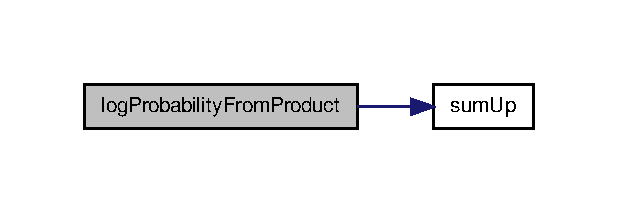
\includegraphics[width=296pt]{common_2measurement_8h_a8df411530d5811c51cb675a64547eed9_cgraph}
\end{center}
\end{figure}


\hypertarget{common_2measurement_8h_abe35a2e2ccf6060635d4daf6d6ebf59e}{\index{common/measurement.\-h@{common/measurement.\-h}!new\-Commutative\-Product@{new\-Commutative\-Product}}
\index{new\-Commutative\-Product@{new\-Commutative\-Product}!common/measurement.h@{common/measurement.\-h}}
\subsubsection[{new\-Commutative\-Product}]{\setlength{\rightskip}{0pt plus 5cm}{\bf \-Commutative\-Product} {\bf new\-Commutative\-Product} (
\begin{DoxyParamCaption}
\item[{size\-\_\-t}]{constants}
\end{DoxyParamCaption}
)}}\label{common_2measurement_8h_abe35a2e2ccf6060635d4daf6d6ebf59e}


creates a new commutative product without any factors 


\begin{DoxyParams}{\-Parameters}
{\em constants} & number of formal constants \\
\hline
\end{DoxyParams}
\begin{DoxyReturn}{\-Returns}
new \-Commutative\-Product object 
\end{DoxyReturn}


\-Definition at line 126 of file measurement.\-c.



\-References s\-Commutative\-Product\-::constants, s\-Commutative\-Product\-::intermediate, s\-Commutative\-Product\-::match, s\-Commutative\-Product\-::mismatch, and \-R\-E\-T\-U\-R\-N\-\_\-\-Z\-E\-R\-O\-\_\-\-I\-F\-\_\-\-Z\-E\-R\-O\-I.



\-Referenced by optimize\-Condition\-Map().


\begin{DoxyCode}
{
    RETURN_ZERO_IF_ZEROI(constants);

    CommutativeProduct p;
    p = malloc(sizeof(struct sCommutativeProduct));

    p->constants = constants;

    p->mismatch = calloc(constants, sizeof(size_t));
    p->match = calloc(constants, sizeof(size_t));

    p->intermediate = malloc(constants * 2 * sizeof(LogProbability));

    return p;
}
\end{DoxyCode}
\hypertarget{common_2measurement_8h_ac4b7705e5a5c82b5d59b67617e6f2dc4}{\index{common/measurement.\-h@{common/measurement.\-h}!new\-Condition\-Map@{new\-Condition\-Map}}
\index{new\-Condition\-Map@{new\-Condition\-Map}!common/measurement.h@{common/measurement.\-h}}
\subsubsection[{new\-Condition\-Map}]{\setlength{\rightskip}{0pt plus 5cm}{\bf \-Condition\-Map} {\bf new\-Condition\-Map} (
\begin{DoxyParamCaption}
\item[{size\-\_\-t}]{objects}
\end{DoxyParamCaption}
)}}\label{common_2measurement_8h_ac4b7705e5a5c82b5d59b67617e6f2dc4}


creates a new condition map 


\begin{DoxyParams}{\-Parameters}
{\em objects} & cardinality of the domain \\
\hline
\end{DoxyParams}
\begin{DoxyReturn}{\-Returns}
new \-Condition\-Map object 
\end{DoxyReturn}


\-Definition at line 168 of file measurement.\-c.



\-References s\-Condition\-Map\-::c, s\-Condition\-Map\-::objects, and \-R\-E\-T\-U\-R\-N\-\_\-\-Z\-E\-R\-O\-\_\-\-I\-F\-\_\-\-Z\-E\-R\-O\-I.



\-Referenced by main().


\begin{DoxyCode}
{
    RETURN_ZERO_IF_ZEROI(objects);

    ConditionMap c;
    c = malloc(sizeof(struct sConditionMap));

    c->objects = objects;
    c->c = calloc(objects, sizeof(size_t));

    return c;
}
\end{DoxyCode}
\hypertarget{common_2measurement_8h_aa0f12091b86c478e159761719923bd9a}{\index{common/measurement.\-h@{common/measurement.\-h}!new\-Eta\-Function@{new\-Eta\-Function}}
\index{new\-Eta\-Function@{new\-Eta\-Function}!common/measurement.h@{common/measurement.\-h}}
\subsubsection[{new\-Eta\-Function}]{\setlength{\rightskip}{0pt plus 5cm}{\bf \-Eta\-Function} {\bf new\-Eta\-Function} (
\begin{DoxyParamCaption}
\item[{size\-\_\-t}]{types, }
\item[{size\-\_\-t}]{measurements, }
\item[{size\-\_\-t}]{constants}
\end{DoxyParamCaption}
)}}\label{common_2measurement_8h_aa0f12091b86c478e159761719923bd9a}


creates a new \-Eta\-Function 


\begin{DoxyParams}{\-Parameters}
{\em types} & number of types, usually 2 \\
\hline
{\em measurements} & number of different measurements, \\
\hline
{\em constants} & number of different error constants, $<$= types$\ast$measurements are needed. \\
\hline
\end{DoxyParams}
\begin{DoxyReturn}{\-Returns}
a new structure 
\end{DoxyReturn}


\-Definition at line 38 of file measurement.\-c.



\-References s\-Eta\-Function\-::\-C, s\-Eta\-Function\-::constants, s\-Eta\-Function\-::eta, s\-Eta\-Function\-::measurements, \-R\-E\-T\-U\-R\-N\-\_\-\-Z\-E\-R\-O\-\_\-\-I\-F\-\_\-\-Z\-E\-R\-O\-I, and s\-Eta\-Function\-::types.



\-Referenced by new\-General\-Eta\-Function(), and new\-Uniform\-Eta\-Function().


\begin{DoxyCode}
{
    RETURN_ZERO_IF_ZEROI(types);
    RETURN_ZERO_IF_ZEROI(measurements);
    RETURN_ZERO_IF_ZEROI(constants);

    EtaFunction e;
    e = malloc(sizeof(struct sEtaFunction));

    e->types = types;
    e->measurements = measurements;
    e->constants = constants;

    e->C = calloc(constants, sizeof(Probability));
    e->eta = calloc(types * measurements, sizeof(size_t));

    return e;
}
\end{DoxyCode}
\hypertarget{common_2measurement_8h_a018a3a7d15c126cbf15d03ba2698fe39}{\index{common/measurement.\-h@{common/measurement.\-h}!new\-General\-Eta\-Function@{new\-General\-Eta\-Function}}
\index{new\-General\-Eta\-Function@{new\-General\-Eta\-Function}!common/measurement.h@{common/measurement.\-h}}
\subsubsection[{new\-General\-Eta\-Function}]{\setlength{\rightskip}{0pt plus 5cm}{\bf \-Eta\-Function} {\bf new\-General\-Eta\-Function} (
\begin{DoxyParamCaption}
\item[{size\-\_\-t}]{types, }
\item[{size\-\_\-t}]{measurements}
\end{DoxyParamCaption}
)}}\label{common_2measurement_8h_a018a3a7d15c126cbf15d03ba2698fe39}


create a new \-Eta\-Function with the a constant for each type and measurement on its own 


\begin{DoxyParams}{\-Parameters}
{\em types} & \\
\hline
{\em measurements} & \\
\hline
\end{DoxyParams}
\begin{DoxyReturn}{\-Returns}

\end{DoxyReturn}


\-Definition at line 104 of file measurement.\-c.



\-References s\-Eta\-Function\-::eta, and new\-Eta\-Function().


\begin{DoxyCode}
{
    EtaFunction e;
    e = newEtaFunction(types, measurements, types * measurements);

    for (size_t t = 0; t < types; ++t)
    {
        for (size_t m = 0; m < measurements; ++m)
        {
            e->eta[t * measurements + m] = t * measurements + m;
        }
    }

    return e;
}
\end{DoxyCode}


\-Here is the call graph for this function\-:\nopagebreak
\begin{figure}[H]
\begin{center}
\leavevmode
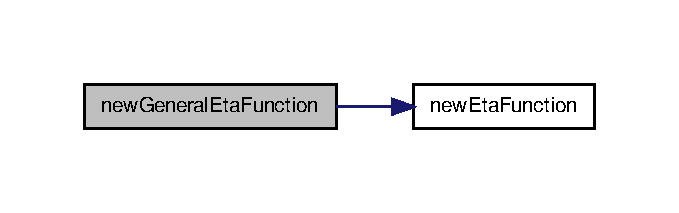
\includegraphics[width=326pt]{common_2measurement_8h_a018a3a7d15c126cbf15d03ba2698fe39_cgraph}
\end{center}
\end{figure}


\hypertarget{common_2measurement_8h_a25fcd9b89607eaa3abe03aea6ffe0447}{\index{common/measurement.\-h@{common/measurement.\-h}!new\-Log\-Cache@{new\-Log\-Cache}}
\index{new\-Log\-Cache@{new\-Log\-Cache}!common/measurement.h@{common/measurement.\-h}}
\subsubsection[{new\-Log\-Cache}]{\setlength{\rightskip}{0pt plus 5cm}{\bf \-Log\-Cache} {\bf new\-Log\-Cache} (
\begin{DoxyParamCaption}
\item[{size\-\_\-t}]{constants}
\end{DoxyParamCaption}
)}}\label{common_2measurement_8h_a25fcd9b89607eaa3abe03aea6ffe0447}


creates a new cache for logs of constants 


\begin{DoxyParams}{\-Parameters}
{\em constants} & number of constants \\
\hline
\end{DoxyParams}
\begin{DoxyReturn}{\-Returns}
new \-Log\-Cache 
\end{DoxyReturn}


\-Definition at line 203 of file measurement.\-c.



\-References s\-Log\-Cache\-::constants, s\-Log\-Cache\-::log\-C, and s\-Log\-Cache\-::log\-Not\-C.



\-Referenced by main().


\begin{DoxyCode}
{
    LogCache l;

    l = malloc(sizeof(struct sLogCache));

    l->constants = constants;

    l->logC = calloc(constants, sizeof(LogProbability));
    l->logNotC = calloc(constants, sizeof(LogProbability));

    return l;
}
\end{DoxyCode}
\hypertarget{common_2measurement_8h_a48c795067056a496c8e4aa903fac7d71}{\index{common/measurement.\-h@{common/measurement.\-h}!new\-Uniform\-Eta\-Function@{new\-Uniform\-Eta\-Function}}
\index{new\-Uniform\-Eta\-Function@{new\-Uniform\-Eta\-Function}!common/measurement.h@{common/measurement.\-h}}
\subsubsection[{new\-Uniform\-Eta\-Function}]{\setlength{\rightskip}{0pt plus 5cm}{\bf \-Eta\-Function} {\bf new\-Uniform\-Eta\-Function} (
\begin{DoxyParamCaption}
\item[{size\-\_\-t}]{types, }
\item[{size\-\_\-t}]{measurements}
\end{DoxyParamCaption}
)}}\label{common_2measurement_8h_a48c795067056a496c8e4aa903fac7d71}


create a new \-Eta\-Function with the same constant for each type 


\begin{DoxyParams}{\-Parameters}
{\em types} & \\
\hline
{\em measurements} & \\
\hline
\end{DoxyParams}
\begin{DoxyReturn}{\-Returns}

\end{DoxyReturn}


\-Definition at line 81 of file measurement.\-c.



\-References s\-Eta\-Function\-::eta, and new\-Eta\-Function().



\-Referenced by main().


\begin{DoxyCode}
{
    EtaFunction e;
    e = newEtaFunction(types, measurements, types);

    for (size_t t = 0; t < types; ++t)
    {
        for (size_t m = 0; m < measurements; ++m)
        {
            e->eta[t * measurements + m] = t;
        }
    }

    return e;
}
\end{DoxyCode}


\-Here is the call graph for this function\-:\nopagebreak
\begin{figure}[H]
\begin{center}
\leavevmode
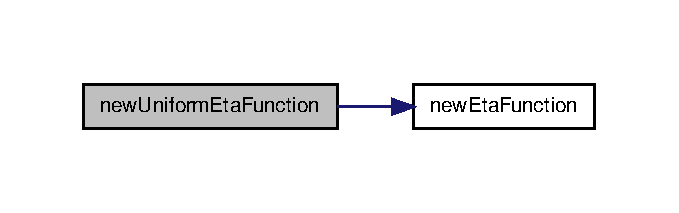
\includegraphics[width=326pt]{common_2measurement_8h_a48c795067056a496c8e4aa903fac7d71_cgraph}
\end{center}
\end{figure}


\hypertarget{common_2measurement_8h_a6ec39ef8a7180bc340afed87c57ca604}{\index{common/measurement.\-h@{common/measurement.\-h}!sum\-Up@{sum\-Up}}
\index{sum\-Up@{sum\-Up}!common/measurement.h@{common/measurement.\-h}}
\subsubsection[{sum\-Up}]{\setlength{\rightskip}{0pt plus 5cm}{\bf \-Log\-Probability} {\bf sum\-Up} (
\begin{DoxyParamCaption}
\item[{const {\bf \-Log\-Probability} $\ast$restrict}]{\-V, }
\item[{size\-\_\-t}]{length, }
\item[{{\bf \-Log\-Probability}}]{lower\-\_\-bound, }
\item[{{\bf \-Log\-Probability}}]{upper\-\_\-bound}
\end{DoxyParamCaption}
)}}\label{common_2measurement_8h_a6ec39ef8a7180bc340afed87c57ca604}


\-This routine calculates the sum of elements of a vector using in place quick sort strategies to branch sums. 


\begin{DoxyParams}{\-Parameters}
{\em \-V} & ptr to array of \-Log\-Probabilities \\
\hline
{\em length} & length of array \-V \\
\hline
{\em lower\-\_\-bound} & lower bound to include in this sum \\
\hline
{\em upper\-\_\-bound} & upper bound to include in this sum \\
\hline
\end{DoxyParams}
\begin{DoxyReturn}{\-Returns}
\[ \sum_{i=0: \mathrm{lower\_bound}\leq V(i) < \mathrm{upper\_bound}}^{ \mathrm{length}} V(i) \] 
\end{DoxyReturn}


\-Definition at line 295 of file measurement.\-c.



\-Referenced by log\-Probability\-From\-Product().


\begin{DoxyCode}
{

}
\end{DoxyCode}

\hypertarget{easy_2measurement_8h}{\section{src/fca/easy/measurement.h \-File \-Reference}
\label{easy_2measurement_8h}\index{src/fca/easy/measurement.\-h@{src/fca/easy/measurement.\-h}}
}
\-This graph shows which files directly or indirectly include this file\-:
\nopagebreak
\begin{figure}[H]
\begin{center}
\leavevmode
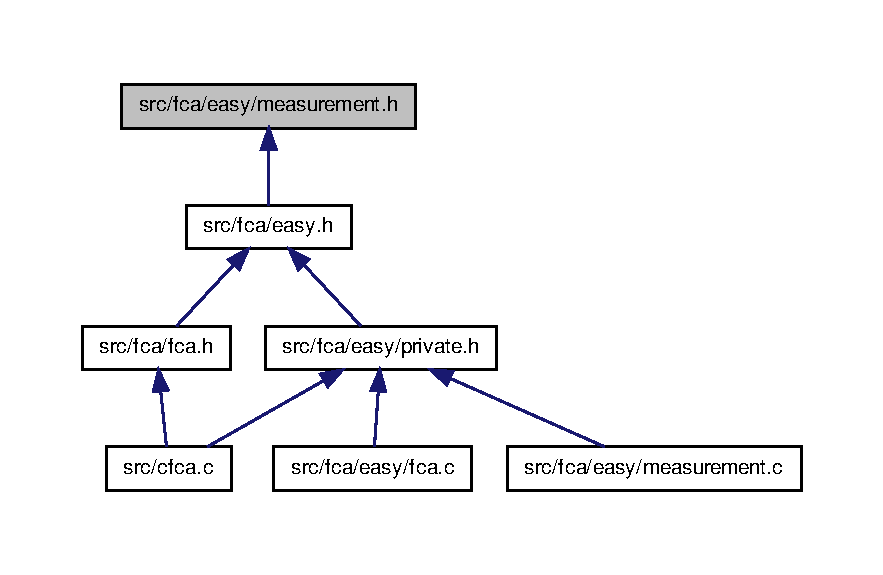
\includegraphics[width=350pt]{easy_2measurement_8h__dep__incl}
\end{center}
\end{figure}
\subsection*{\-Functions}
\begin{DoxyCompactItemize}
\item 
void \hyperlink{easy_2measurement_8h_a0d243c594867f254694b0a91409d9b87}{calculate\-Likelihood} (const \hyperlink{easy_8h_ad53dc3fc96151a44387245e6481f95a4}{\-Formal\-Context} \-B, const \hyperlink{common_2measurement_8h_ad29ab52c5830e8da1f1327d6e3fb1d64}{\-Condition\-Map} c, const \hyperlink{easy_8h_ad53dc3fc96151a44387245e6481f95a4}{\-Formal\-Context} \-I, const \hyperlink{common_2measurement_8h_ab2406aaef0ce3e9f38a79f42ce470ffb}{\-Eta\-Function} eta, \hyperlink{common_2measurement_8h_afb8ffb8c068ef8c9fa3677762ac85994}{\-Commutative\-Product} \-L)
\begin{DoxyCompactList}\small\item\em \hyperlink{easy_2measurement_8h}{easy/measurement.\-h}, (c) 2013, \-Immanuel \-Albrecht; \-Dresden \-University of \-Technology, \-Professur für die \-Psychologie des \-Lernen und \-Lehrens \end{DoxyCompactList}\item 
\hyperlink{easy_8h_ad53dc3fc96151a44387245e6481f95a4}{\-Formal\-Context} \hyperlink{easy_2measurement_8h_af5995b46b1b93746a2cf6af36ce00aed}{new\-Fake\-Measurement} (const \hyperlink{easy_8h_ad53dc3fc96151a44387245e6481f95a4}{\-Formal\-Context} \-I, const \hyperlink{common_2measurement_8h_ab2406aaef0ce3e9f38a79f42ce470ffb}{\-Eta\-Function} eta, int experiments)
\begin{DoxyCompactList}\small\item\em generates a new formal context that comprises of a pseudo-\/random fake measurement obtained from \-I with the given error probabilites and experiment count \end{DoxyCompactList}\end{DoxyCompactItemize}


\subsection{\-Function \-Documentation}
\hypertarget{easy_2measurement_8h_a0d243c594867f254694b0a91409d9b87}{\index{easy/measurement.\-h@{easy/measurement.\-h}!calculate\-Likelihood@{calculate\-Likelihood}}
\index{calculate\-Likelihood@{calculate\-Likelihood}!easy/measurement.h@{easy/measurement.\-h}}
\subsubsection[{calculate\-Likelihood}]{\setlength{\rightskip}{0pt plus 5cm}void {\bf calculate\-Likelihood} (
\begin{DoxyParamCaption}
\item[{const {\bf \-Formal\-Context}}]{\-B, }
\item[{const {\bf \-Condition\-Map}}]{c, }
\item[{const {\bf \-Formal\-Context}}]{\-I, }
\item[{const {\bf \-Eta\-Function}}]{eta, }
\item[{{\bf \-Commutative\-Product}}]{\-L}
\end{DoxyParamCaption}
)}}\label{easy_2measurement_8h_a0d243c594867f254694b0a91409d9b87}


\hyperlink{easy_2measurement_8h}{easy/measurement.\-h}, (c) 2013, \-Immanuel \-Albrecht; \-Dresden \-University of \-Technology, \-Professur für die \-Psychologie des \-Lernen und \-Lehrens 

\-This program is free software\-: you can redistribute it and/or modify it under the terms of the \-G\-N\-U \-General \-Public \-License as published by the \-Free \-Software \-Foundation, either version 3 of the \-License, or (at your option) any later version.

\-This program is distributed in the hope that it will be useful, but \-W\-I\-T\-H\-O\-U\-T \-A\-N\-Y \-W\-A\-R\-R\-A\-N\-T\-Y; without even the implied warranty of \-M\-E\-R\-C\-H\-A\-N\-T\-A\-B\-I\-L\-I\-T\-Y or \-F\-I\-T\-N\-E\-S\-S \-F\-O\-R \-A \-P\-A\-R\-T\-I\-C\-U\-L\-A\-R \-P\-U\-R\-P\-O\-S\-E. \-See the \-G\-N\-U \-General \-Public \-License for more details.

\-You should have received a copy of the \-G\-N\-U \-General \-Public \-License along with this program. \-If not, see $<$\href{http://www.gnu.org/licenses/}{\tt http\-://www.\-gnu.\-org/licenses/}$>$.

\hyperlink{easy_2measurement_8h}{easy/measurement.\-h}, (c) 2013, \-Immanuel \-Albrecht; \-Dresden \-University of \-Technology, \-Professur für die \-Psychologie des \-Lernen und \-Lehrens

\-This program is free software\-: you can redistribute it and/or modify it under the terms of the \-G\-N\-U \-General \-Public \-License as published by the \-Free \-Software \-Foundation, either version 3 of the \-License, or (at your option) any later version.

\-This program is distributed in the hope that it will be useful, but \-W\-I\-T\-H\-O\-U\-T \-A\-N\-Y \-W\-A\-R\-R\-A\-N\-T\-Y; without even the implied warranty of \-M\-E\-R\-C\-H\-A\-N\-T\-A\-B\-I\-L\-I\-T\-Y or \-F\-I\-T\-N\-E\-S\-S \-F\-O\-R \-A \-P\-A\-R\-T\-I\-C\-U\-L\-A\-R \-P\-U\-R\-P\-O\-S\-E. \-See the \-G\-N\-U \-General \-Public \-License for more details.

\-You should have received a copy of the \-G\-N\-U \-General \-Public \-License along with this program. \-If not, see $<$\href{http://www.gnu.org/licenses/}{\tt http\-://www.\-gnu.\-org/licenses/}$>$. calculates the likelihood function \-L 
\begin{DoxyParams}{\-Parameters}
{\em \-B} & the measurement context \\
\hline
{\em c} & the condition map (mapping objects \\
\hline
{\em \-I} & \\
\hline
{\em eta} & \\
\hline
{\em \-L} & \\
\hline
\end{DoxyParams}


\-Definition at line 34 of file measurement.\-c.



\-References s\-Condition\-Map\-::c, s\-Eta\-Function\-::constants, s\-Commutative\-Product\-::constants, s\-Eta\-Function\-::eta, g\-Im, s\-Commutative\-Product\-::match, s\-Eta\-Function\-::measurements, s\-Commutative\-Product\-::mismatch, s\-Condition\-Map\-::objects, \-R\-E\-T\-U\-R\-N\-\_\-\-I\-F\-\_\-\-Z\-E\-R\-O, s\-Eta\-Function\-::types, \-W\-A\-R\-N\-\_\-\-I\-F\-\_\-\-G\-E\-Q\-\_\-\-D\-O, and \-W\-A\-R\-N\-\_\-\-I\-F\-\_\-\-U\-N\-E\-Q\-U\-A\-L\-\_\-\-D\-O.


\begin{DoxyCode}
{
    RETURN_IF_ZERO(B);
    RETURN_IF_ZERO(c);
    RETURN_IF_ZERO(I);
    RETURN_IF_ZERO(eta);
    RETURN_IF_ZERO(L);

    const myFormalContext* restrict b;
    b = (const myFormalContext*) B;

    const myFormalContext* restrict i;
    i = (const myFormalContext*) I;

    WARN_IF_UNEQUAL_DO(b->objects, (int )c->objects, return);
    WARN_IF_UNEQUAL_DO(b->attributes, i->attributes, return);
    WARN_IF_UNEQUAL_DO(i->attributes, (int ) eta->measurements, return);
    WARN_IF_UNEQUAL_DO(2, eta->types, return);
    WARN_IF_UNEQUAL_DO(eta->constants, L->constants,);

    memset(L->match, 0, sizeof(size_t) * L->constants);
    memset(L->mismatch, 0, sizeof(size_t) * L->constants);

    for (int g = 0; g < b->objects; ++g)
    {
        int c_g;
        c_g = (int) c->c[g];

        WARN_IF_GEQ_DO(c_g, i->objects, continue);

        for (int m = 0; m < b->attributes; ++m)
        {
            if (gIm(c_g,i,m))
            {
                if (gIm(g,b,m))
                {
                    L->match[eta->eta[b->attributes + m]]++;
                }
                else
                {
                    L->mismatch[eta->eta[b->attributes + m]]++;
                }
            }
            else
            {
                if (gIm(g,b,m))
                {
                    L->mismatch[eta->eta[m]]++;
                }
                else
                {
                    L->match[eta->eta[m]]++;
                }
            }
        }
    }
}
\end{DoxyCode}
\hypertarget{easy_2measurement_8h_af5995b46b1b93746a2cf6af36ce00aed}{\index{easy/measurement.\-h@{easy/measurement.\-h}!new\-Fake\-Measurement@{new\-Fake\-Measurement}}
\index{new\-Fake\-Measurement@{new\-Fake\-Measurement}!easy/measurement.h@{easy/measurement.\-h}}
\subsubsection[{new\-Fake\-Measurement}]{\setlength{\rightskip}{0pt plus 5cm}{\bf \-Formal\-Context} {\bf new\-Fake\-Measurement} (
\begin{DoxyParamCaption}
\item[{const {\bf \-Formal\-Context}}]{\-I, }
\item[{const {\bf \-Eta\-Function}}]{eta, }
\item[{int}]{experiments}
\end{DoxyParamCaption}
)}}\label{easy_2measurement_8h_af5995b46b1b93746a2cf6af36ce00aed}


generates a new formal context that comprises of a pseudo-\/random fake measurement obtained from \-I with the given error probabilites and experiment count 


\begin{DoxyParams}{\-Parameters}
{\em \-I} & experimental condition context \\
\hline
{\em eta} & error probabilities \\
\hline
{\em experiments} & number of conducted experiments \\
\hline
\end{DoxyParams}
\begin{DoxyReturn}{\-Returns}
a new \-Formal\-Context object 
\end{DoxyReturn}


\-Definition at line 102 of file measurement.\-c.



\-References s\-Eta\-Function\-::\-C, \-C\-E\-L\-L, \-C\-R\-O\-S\-S, s\-Eta\-Function\-::eta, g\-Im, s\-Eta\-Function\-::measurements, \-M\-I\-N, new\-Formal\-Context, \-R\-E\-T\-U\-R\-N\-\_\-\-Z\-E\-R\-O\-\_\-\-I\-F\-\_\-\-Z\-E\-R\-O, and \-W\-A\-R\-N\-\_\-\-I\-F\-\_\-\-U\-N\-E\-Q\-U\-A\-L\-\_\-\-D\-O.



\-Referenced by main().


\begin{DoxyCode}
{
    RETURN_ZERO_IF_ZERO(I);
    RETURN_ZERO_IF_ZERO(eta);

    const myFormalContext* restrict i;
    i = (const myFormalContext*) I;

    WARN_IF_UNEQUAL_DO(i->attributes, (int ) eta->measurements, return 0);

    myFormalContext *b;
    b = (myFormalContext *) newFormalContext(experiments, i->attributes);

    for (int x = 0; x < experiments; ++x)
    {
        int c_x;
        c_x =
                MIN((int) floor((double) (random()) /
                                (double) RAND_MAX * (double)i->objects), i->
      objects-1);


        for (int m = 0; m < i->attributes; ++m)
        {
            Probability rnd;
            rnd = (Probability) random() / (Probability) RAND_MAX;

            if (gIm(c_x,i,m))
            {
                if (rnd >= eta->C[eta->eta[i->attributes + m]])
                    CROSS(CELL(x,b,m));
            }
            else
            {
                if (rnd < eta->C[eta->eta[m]])
                    CROSS(CELL(x,b,m));
            }
        }
    }

    return (FormalContext) b;
}
\end{DoxyCode}

\hypertarget{vector_2measurement_8h}{\section{src/fca/vector/measurement.h \-File \-Reference}
\label{vector_2measurement_8h}\index{src/fca/vector/measurement.\-h@{src/fca/vector/measurement.\-h}}
}

\hypertarget{easy_8h}{\section{src/fca/easy.h \-File \-Reference}
\label{easy_8h}\index{src/fca/easy.\-h@{src/fca/easy.\-h}}
}


\hyperlink{easy_8h}{easy.\-h}, (c) 2013, \-Immanuel \-Albrecht; \-Dresden \-University of \-Technology, \-Professur für die \-Psychologie des \-Lernen und \-Lehrens  


{\ttfamily \#include $<$inttypes.\-h$>$}\*
{\ttfamily \#include \char`\"{}common.\-h\char`\"{}}\*
{\ttfamily \#include \char`\"{}easy/macros.\-h\char`\"{}}\*
\-Include dependency graph for easy.\-h\-:
\nopagebreak
\begin{figure}[H]
\begin{center}
\leavevmode
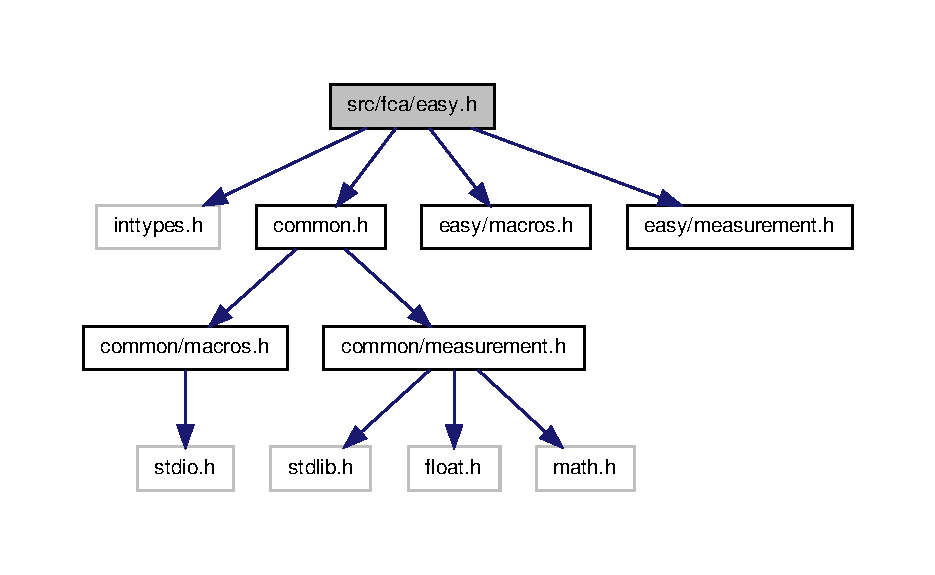
\includegraphics[width=323pt]{easy_8h__incl}
\end{center}
\end{figure}
\-This graph shows which files directly or indirectly include this file\-:\nopagebreak
\begin{figure}[H]
\begin{center}
\leavevmode
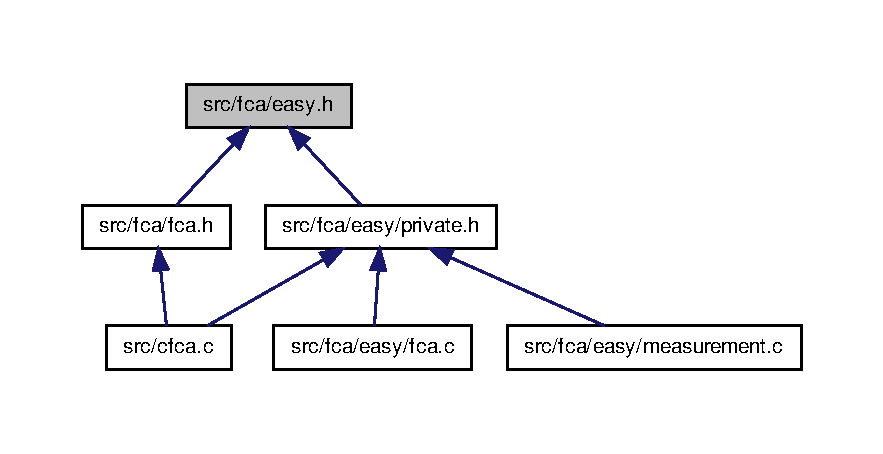
\includegraphics[width=278pt]{easy_8h__dep__incl}
\end{center}
\end{figure}
\subsection*{\-Data \-Structures}
\begin{DoxyCompactItemize}
\item 
struct \hyperlink{structsFormalIntent}{s\-Formal\-Intent}
\begin{DoxyCompactList}\small\item\em intent structure of a formal concept \end{DoxyCompactList}\end{DoxyCompactItemize}
\subsection*{\-Typedefs}
\begin{DoxyCompactItemize}
\item 
typedef int8\-\_\-t \hyperlink{easy_8h_a92fa84ef7a12663bb998f141ab729056}{\-Incidence\-Cell}
\begin{DoxyCompactList}\small\item\em type of the incidence relation matrix cells \end{DoxyCompactList}\item 
typedef struct \hyperlink{safeguard_8h_acb2286fcdcd7730dc267d726fa84305b}{s\-Formal\-Context} $\ast$ \hyperlink{easy_8h_ad53dc3fc96151a44387245e6481f95a4}{\-Formal\-Context}
\item 
typedef struct \hyperlink{structsFormalIntent}{s\-Formal\-Intent} \hyperlink{easy_8h_a78ba8f8456c0a3d9a891d93945f2664b}{\-Formal\-Intent}
\begin{DoxyCompactList}\small\item\em intent structure of a formal concept \end{DoxyCompactList}\end{DoxyCompactItemize}
\subsection*{\-Functions}
\begin{DoxyCompactItemize}
\item 
\hyperlink{easy_8h_ad53dc3fc96151a44387245e6481f95a4}{\-Formal\-Context} \hyperlink{easy_8h_a8cc0086fc3f45b783688b21105632456}{new\-Formal\-Context} (int objects, int attributes)
\begin{DoxyCompactList}\small\item\em create a new formal context \end{DoxyCompactList}\item 
\hyperlink{easy_8h_ad53dc3fc96151a44387245e6481f95a4}{\-Formal\-Context} \hyperlink{easy_8h_ae3105d9c1d91e1816c8b7a83d3414790}{new\-Formal\-Context\-From\-Random} (int objects, int attributes, float p)
\begin{DoxyCompactList}\small\item\em create a new formal context with random incidence relation \end{DoxyCompactList}\item 
\hyperlink{easy_8h_ad53dc3fc96151a44387245e6481f95a4}{\-Formal\-Context} \hyperlink{easy_8h_af3e05ebca016a7d4d09b332eac01a456}{new\-Formal\-Context\-From\-File} (const char $\ast$filename)
\begin{DoxyCompactList}\small\item\em create a new formal context object from a .cxt file \end{DoxyCompactList}\item 
int \hyperlink{easy_8h_aaf6da61c84352d127039536dd6e790b6}{count\-Context\-Concepts} (\hyperlink{easy_8h_ad53dc3fc96151a44387245e6481f95a4}{\-Formal\-Context} ctx)
\begin{DoxyCompactList}\small\item\em counts the concepts in the concept lattice of ctx, using next closure algorithm \end{DoxyCompactList}\item 
void \hyperlink{easy_8h_a064800878bf96c6398d2f716609df081}{write\-Formal\-Context} (\hyperlink{easy_8h_ad53dc3fc96151a44387245e6481f95a4}{\-Formal\-Context} ctx, const char $\ast$filename)
\begin{DoxyCompactList}\small\item\em save the context ctx at the given file location \end{DoxyCompactList}\item 
void \hyperlink{easy_8h_a9835be78a56a9eaec5346a86562f10c3}{delete\-Formal\-Context} (\hyperlink{easy_8h_ad53dc3fc96151a44387245e6481f95a4}{\-Formal\-Context} $\ast$ctx)
\begin{DoxyCompactList}\small\item\em deletes the formal context $\ast$ctx, and sets the pointer to zero \end{DoxyCompactList}\end{DoxyCompactItemize}


\subsection{\-Detailed \-Description}
\hyperlink{easy_8h}{easy.\-h}, (c) 2013, \-Immanuel \-Albrecht; \-Dresden \-University of \-Technology, \-Professur für die \-Psychologie des \-Lernen und \-Lehrens \-This program is free software\-: you can redistribute it and/or modify it under the terms of the \-G\-N\-U \-General \-Public \-License as published by the \-Free \-Software \-Foundation, either version 3 of the \-License, or (at your option) any later version.

\-This program is distributed in the hope that it will be useful, but \-W\-I\-T\-H\-O\-U\-T \-A\-N\-Y \-W\-A\-R\-R\-A\-N\-T\-Y; without even the implied warranty of \-M\-E\-R\-C\-H\-A\-N\-T\-A\-B\-I\-L\-I\-T\-Y or \-F\-I\-T\-N\-E\-S\-S \-F\-O\-R \-A \-P\-A\-R\-T\-I\-C\-U\-L\-A\-R \-P\-U\-R\-P\-O\-S\-E. \-See the \-G\-N\-U \-General \-Public \-License for more details.

\-You should have received a copy of the \-G\-N\-U \-General \-Public \-License along with this program. \-If not, see $<$\href{http://www.gnu.org/licenses/}{\tt http\-://www.\-gnu.\-org/licenses/}$>$.

\-This header file provides interfaces with the easy \-Incidence\-Cell$\ast$ implementations 

\-Definition in file \hyperlink{easy_8h_source}{easy.\-h}.



\subsection{\-Typedef \-Documentation}
\hypertarget{easy_8h_ad53dc3fc96151a44387245e6481f95a4}{\index{easy.\-h@{easy.\-h}!\-Formal\-Context@{\-Formal\-Context}}
\index{\-Formal\-Context@{\-Formal\-Context}!easy.h@{easy.\-h}}
\subsubsection[{\-Formal\-Context}]{\setlength{\rightskip}{0pt plus 5cm}typedef struct {\bf s\-Formal\-Context}$\ast$ {\bf \-Formal\-Context}}}\label{easy_8h_ad53dc3fc96151a44387245e6481f95a4}


\-Definition at line 42 of file easy.\-h.

\hypertarget{easy_8h_a78ba8f8456c0a3d9a891d93945f2664b}{\index{easy.\-h@{easy.\-h}!\-Formal\-Intent@{\-Formal\-Intent}}
\index{\-Formal\-Intent@{\-Formal\-Intent}!easy.h@{easy.\-h}}
\subsubsection[{\-Formal\-Intent}]{\setlength{\rightskip}{0pt plus 5cm}typedef struct {\bf s\-Formal\-Intent}  {\bf \-Formal\-Intent}}}\label{easy_8h_a78ba8f8456c0a3d9a891d93945f2664b}


intent structure of a formal concept 

\hypertarget{easy_8h_a92fa84ef7a12663bb998f141ab729056}{\index{easy.\-h@{easy.\-h}!\-Incidence\-Cell@{\-Incidence\-Cell}}
\index{\-Incidence\-Cell@{\-Incidence\-Cell}!easy.h@{easy.\-h}}
\subsubsection[{\-Incidence\-Cell}]{\setlength{\rightskip}{0pt plus 5cm}typedef int8\-\_\-t {\bf \-Incidence\-Cell}}}\label{easy_8h_a92fa84ef7a12663bb998f141ab729056}


type of the incidence relation matrix cells 



\-Definition at line 35 of file easy.\-h.



\subsection{\-Function \-Documentation}
\hypertarget{easy_8h_aaf6da61c84352d127039536dd6e790b6}{\index{easy.\-h@{easy.\-h}!count\-Context\-Concepts@{count\-Context\-Concepts}}
\index{count\-Context\-Concepts@{count\-Context\-Concepts}!easy.h@{easy.\-h}}
\subsubsection[{count\-Context\-Concepts}]{\setlength{\rightskip}{0pt plus 5cm}int {\bf count\-Context\-Concepts} (
\begin{DoxyParamCaption}
\item[{{\bf \-Formal\-Context}}]{ctx}
\end{DoxyParamCaption}
)}}\label{easy_8h_aaf6da61c84352d127039536dd6e790b6}


counts the concepts in the concept lattice of ctx, using next closure algorithm 


\begin{DoxyParams}{\-Parameters}
{\em ctx} & formal context \\
\hline
\end{DoxyParams}
\begin{DoxyReturn}{\-Returns}
number of concepts in context 
\end{DoxyReturn}


\-Definition at line 926 of file fca.\-c.



\-References smy\-Formal\-Context\-::attributes, \-C\-L\-E\-A\-R, close\-Intent, \-C\-R\-O\-S\-S, \-I\-N\-C\-I\-D\-E\-S, and \-R\-E\-T\-U\-R\-N\-\_\-\-Z\-E\-R\-O\-\_\-\-I\-F\-\_\-\-Z\-E\-R\-O.


\begin{DoxyCode}
{
    RETURN_ZERO_IF_ZERO(ctx);

    myFormalContext *c;
    c = (myFormalContext*) ctx;

    IncidenceCell *M;
    IncidenceCell *Y;

#pragma GCC diagnostic push
#pragma GCC diagnostic ignored "-Wsign-conversion"

    Y = calloc(c->attributes, sizeof(IncidenceCell));
    M = malloc(c->attributes * sizeof(IncidenceCell));

#pragma GCC diagnostic pop

    /*
     * calculate the bottom intent of the concept lattice, i.e. {}''
     */
    closeIntent(ctx, Y, M);

    int count;

    count = 1;

    /*
     * begin of nextClosure function iteration
     */
    nextClosure:

    for (int i = c->attributes - 1; i >= 0; --i)
    {

        if (!INCIDES(M[i]))
        {
            CROSS(M[i]);
            closeIntent(ctx, M, Y);

            int good;
            good = 1;

            for (int j = 0; j < i; ++j)
            {
                if (INCIDES(Y[j]))
                {
                    if (!INCIDES((M[j])))
                    {

                        good = 0;
                        break;
                    }
                }
            }
            if (good)
            {
                /*
                 * we found the next intent
                 */
                count++;

                /*
                 * continue with Y for M
                 */

                IncidenceCell *DELTA;
                DELTA = M;
                M = Y;
                Y = DELTA;
                /*
                 * do the nextClosure
                 */
                goto nextClosure;
            }
        }

        CLEAR(M[i]);
    }

    /*
     * free up memory
     */

    free(M);
    free(Y);

    return count;
}
\end{DoxyCode}
\hypertarget{easy_8h_a9835be78a56a9eaec5346a86562f10c3}{\index{easy.\-h@{easy.\-h}!delete\-Formal\-Context@{delete\-Formal\-Context}}
\index{delete\-Formal\-Context@{delete\-Formal\-Context}!easy.h@{easy.\-h}}
\subsubsection[{delete\-Formal\-Context}]{\setlength{\rightskip}{0pt plus 5cm}void {\bf delete\-Formal\-Context} (
\begin{DoxyParamCaption}
\item[{{\bf \-Formal\-Context} $\ast$}]{ctx}
\end{DoxyParamCaption}
)}}\label{easy_8h_a9835be78a56a9eaec5346a86562f10c3}


deletes the formal context $\ast$ctx, and sets the pointer to zero 


\begin{DoxyParams}{\-Parameters}
{\em ctx} & pointer to the formal context object to be deleted \\
\hline
\end{DoxyParams}


\-Definition at line 264 of file fca.\-c.



\-References smy\-Formal\-Context\-::attribute\-Names, smy\-Formal\-Context\-::attributes, smy\-Formal\-Context\-::incidence, smy\-Formal\-Context\-::object\-Names, smy\-Formal\-Context\-::objects, and \-R\-E\-T\-U\-R\-N\-\_\-\-I\-F\-\_\-\-Z\-E\-R\-O.


\begin{DoxyCode}
{
    RETURN_IF_ZERO(ctx);
    RETURN_IF_ZERO(*ctx);

    myFormalContext *c;

    c = (myFormalContext*) *ctx;

    *ctx = 0;

    for (int var = 0; var < c->attributes; ++var)
    {
        free(c->attributeNames[var]);
    }

    for (int var = 0; var < c->objects; ++var)
    {
        free(c->objectNames[var]);
    }

    free(c->objectNames);
    free(c->attributeNames);
    free(c->incidence);
    free(c);
}
\end{DoxyCode}
\hypertarget{easy_8h_a8cc0086fc3f45b783688b21105632456}{\index{easy.\-h@{easy.\-h}!new\-Formal\-Context@{new\-Formal\-Context}}
\index{new\-Formal\-Context@{new\-Formal\-Context}!easy.h@{easy.\-h}}
\subsubsection[{new\-Formal\-Context}]{\setlength{\rightskip}{0pt plus 5cm}{\bf \-Formal\-Context} {\bf new\-Formal\-Context} (
\begin{DoxyParamCaption}
\item[{int}]{objects, }
\item[{int}]{attributes}
\end{DoxyParamCaption}
)}}\label{easy_8h_a8cc0086fc3f45b783688b21105632456}


create a new formal context 


\begin{DoxyParams}{\-Parameters}
{\em objects} & object count \\
\hline
{\em attributes} & attribute count \\
\hline
\end{DoxyParams}
\begin{DoxyReturn}{\-Returns}
a new \-Formal\-Context object 
\end{DoxyReturn}


\-Definition at line 38 of file fca.\-c.



\-References smy\-Formal\-Context\-::attribute\-Names, smy\-Formal\-Context\-::attributes, smy\-Formal\-Context\-::incidence, smy\-Formal\-Context\-::object\-Names, and smy\-Formal\-Context\-::objects.


\begin{DoxyCode}
{
    myFormalContext *ctx = malloc(sizeof(myFormalContext));

    ctx->attributes = attributes;
    ctx->objects = objects;

#pragma GCC diagnostic push
#pragma GCC diagnostic ignored "-Wsign-conversion"

    ctx->attributeNames = calloc(attributes, sizeof(char*));
    ctx->objectNames = calloc(objects, sizeof(char*));

#pragma GCC diagnostic pop

    for (int var = 0; var < attributes; ++var)
    {
        ctx->attributeNames[var] = calloc(1, sizeof(char));
    }

    for (int var = 0; var < objects; ++var)
    {
        ctx->objectNames[var] = calloc(1, sizeof(char));
    }

#pragma GCC diagnostic push
#pragma GCC diagnostic ignored "-Wsign-conversion"

    ctx->incidence = calloc(objects * attributes, sizeof(IncidenceCell));

#pragma GCC diagnostic pop

    return (FormalContext) ctx;
}
\end{DoxyCode}
\hypertarget{easy_8h_af3e05ebca016a7d4d09b332eac01a456}{\index{easy.\-h@{easy.\-h}!new\-Formal\-Context\-From\-File@{new\-Formal\-Context\-From\-File}}
\index{new\-Formal\-Context\-From\-File@{new\-Formal\-Context\-From\-File}!easy.h@{easy.\-h}}
\subsubsection[{new\-Formal\-Context\-From\-File}]{\setlength{\rightskip}{0pt plus 5cm}{\bf \-Formal\-Context} {\bf new\-Formal\-Context\-From\-File} (
\begin{DoxyParamCaption}
\item[{const char $\ast$}]{filename}
\end{DoxyParamCaption}
)}}\label{easy_8h_af3e05ebca016a7d4d09b332eac01a456}


create a new formal context object from a .cxt file 


\begin{DoxyParams}{\-Parameters}
{\em filename} & \\
\hline
\end{DoxyParams}
\begin{DoxyReturn}{\-Returns}
the formal context that has been read from the given file 
\end{DoxyReturn}


\-Definition at line 80 of file fca.\-c.



\-References smy\-Formal\-Context\-::attribute\-Names, \-C\-E\-L\-L, \-C\-R\-O\-S\-S, \-I\-N\-P\-U\-T\-B\-U\-F\-F\-E\-R\-S\-I\-Z\-E, \-M\-I\-N, new\-Formal\-Context, smy\-Formal\-Context\-::object\-Names, and \-R\-E\-T\-U\-R\-N\-\_\-\-Z\-E\-R\-O\-\_\-\-I\-F\-\_\-\-Z\-E\-R\-O.


\begin{DoxyCode}
{
    char *line;
    size_t len;

    len = (INPUTBUFFERSIZE);
    line = malloc(sizeof(char) * len);

    FILE *file;

    if (strcmp(filename, "-") == 0)
    {
        file = stdin;
    }
    else
    {
        file = fopen(filename, "r");
        RETURN_ZERO_IF_ZERO(file);
    }

    ssize_t read;

    int line_nbr;
    line_nbr = 0;

    int objects;
    int attributes;

    attributes = 0;
    objects = 0;

    myFormalContext *ctx;
    ctx = 0;

    while ((read = getline(&line, &len, file)) != -1)
    {

        /*
         * this should never happen, right?
         */
        if (read == 0)
            break;
        line[read - 1] = 0;

        if (line_nbr == 0)
        {
            if (strcmp(line, "B"))
            {
                fprintf(stderr, "File '%s' is not a .cxt file\n", filename);
                goto grace;
            }
        }
        else if (line_nbr == 1)
        {
            //empty line
        }
        else if (line_nbr == 2)
        {
            objects = atoi(line);
        }
        else if (line_nbr == 3)
        {
            attributes = atoi(line);
            ctx = (myFormalContext *) newFormalContext(objects, attributes);
        }
        else if (line_nbr == 4)
        {
            //empty line
        }
        else if (line_nbr < objects + 5)
        {

            int i;
            i = line_nbr - 5;

            free(ctx->objectNames[i]);
            ctx->objectNames[i] = strdup(line);

        }
        else if (line_nbr < objects + attributes + 5)
        {
            int i;
            i = line_nbr - 5 - objects;

            free(ctx->attributeNames[i]);
            ctx->attributeNames[i] = strdup(line);
        }
        else if (line_nbr < objects * 2 + attributes + 5)
        {
            int i;
            i = line_nbr - 5 - objects - attributes;

            int width;
            width = MIN((signed)strlen(line),attributes);

            for (int var = 0; var < width; ++var)
            {
                if ((line[var] == 'x') || (line[var] == 'X')
                        || (line[var] == '1'))
                {
                    CROSS(CELL (i, ctx, var));
                }
            }

        }
        else
        {
            /*
             * we read all data
             */
            break;
        }

        line_nbr++;
    }

    /*
     * free memory and return
     */

    grace: if (file != stdin)
    {
        fclose(file);
    }

    free(line);

    return (FormalContext) ctx;
}
\end{DoxyCode}
\hypertarget{easy_8h_ae3105d9c1d91e1816c8b7a83d3414790}{\index{easy.\-h@{easy.\-h}!new\-Formal\-Context\-From\-Random@{new\-Formal\-Context\-From\-Random}}
\index{new\-Formal\-Context\-From\-Random@{new\-Formal\-Context\-From\-Random}!easy.h@{easy.\-h}}
\subsubsection[{new\-Formal\-Context\-From\-Random}]{\setlength{\rightskip}{0pt plus 5cm}{\bf \-Formal\-Context} {\bf new\-Formal\-Context\-From\-Random} (
\begin{DoxyParamCaption}
\item[{int}]{objects, }
\item[{int}]{attributes, }
\item[{float}]{p}
\end{DoxyParamCaption}
)}}\label{easy_8h_ae3105d9c1d91e1816c8b7a83d3414790}


create a new formal context with random incidence relation 


\begin{DoxyParams}{\-Parameters}
{\em objects} & \\
\hline
{\em attributes} & \\
\hline
{\em p} & probability of a cross \\
\hline
\end{DoxyParams}
\begin{DoxyReturn}{\-Returns}
context 
\end{DoxyReturn}


\-Definition at line 798 of file fca.\-c.



\-References smy\-Formal\-Context\-::attributes, \-C\-E\-L\-L, \-C\-R\-O\-S\-S, new\-Formal\-Context, and smy\-Formal\-Context\-::objects.


\begin{DoxyCode}
{
    FormalContext ctx;
    ctx = newFormalContext(objects, attributes);

    myFormalContext *c;

    c = (myFormalContext*) ctx;

    for (int g = 0; g < c->objects; ++g)
    {
        for (int m = 0; m < c->attributes; ++m)
        {
            float x;
            x = (float) random() / (float) RAND_MAX;
            if (x >= p)
            {
                CROSS(CELL(g,c,m));
            }
        }
    }
    return ctx;
}
\end{DoxyCode}
\hypertarget{easy_8h_a064800878bf96c6398d2f716609df081}{\index{easy.\-h@{easy.\-h}!write\-Formal\-Context@{write\-Formal\-Context}}
\index{write\-Formal\-Context@{write\-Formal\-Context}!easy.h@{easy.\-h}}
\subsubsection[{write\-Formal\-Context}]{\setlength{\rightskip}{0pt plus 5cm}void {\bf write\-Formal\-Context} (
\begin{DoxyParamCaption}
\item[{{\bf \-Formal\-Context}}]{ctx, }
\item[{const char $\ast$}]{filename}
\end{DoxyParamCaption}
)}}\label{easy_8h_a064800878bf96c6398d2f716609df081}


save the context ctx at the given file location 


\begin{DoxyParams}{\-Parameters}
{\em ctx} & \\
\hline
{\em filename} & \\
\hline
\end{DoxyParams}


\-Definition at line 216 of file fca.\-c.



\-References smy\-Formal\-Context\-::attribute\-Names, smy\-Formal\-Context\-::attributes, g\-Im, smy\-Formal\-Context\-::object\-Names, smy\-Formal\-Context\-::objects, and \-R\-E\-T\-U\-R\-N\-\_\-\-I\-F\-\_\-\-Z\-E\-R\-O.


\begin{DoxyCode}
{
    RETURN_IF_ZERO(ctx);
    RETURN_IF_ZERO(filename);

    FILE* file;
    file = fopen(filename, "w");

    RETURN_IF_ZERO(file);

    myFormalContext *c;
    c = (myFormalContext*) ctx;

    fprintf(file, "B\n\n%d\n%d\n\n", c->objects, c->attributes);

    for (int var = 0; var < c->objects; ++var)
    {
        fputs(c->objectNames[var], file);
        fputs("\n", file);
    }

    for (int var = 0; var < c->attributes; ++var)
    {
        fputs(c->attributeNames[var], file);
        fputs("\n", file);
    }

    for (int g = 0; g < c->objects; ++g)
    {
        for (int m = 0; m < c->attributes; ++m)
        {
            if ( gIm(g, c, m))
                fputs("X", file);
            else
                fputs(".", file);
        }
        fputs("\n", file);
    }

    fclose(file);
}
\end{DoxyCode}

\hypertarget{fca_8c}{\section{src/easy/fca.c \-File \-Reference}
\label{fca_8c}\index{src/easy/fca.\-c@{src/easy/fca.\-c}}
}


\hyperlink{fca_8c}{fca.\-c}, (c) 2013, \-Immanuel \-Albrecht; \-Dresden \-University of \-Technology, \-Professur für die \-Psychologie des \-Lernen und \-Lehrens  


{\ttfamily \#include $<$stdio.\-h$>$}\*
{\ttfamily \#include $<$stdlib.\-h$>$}\*
{\ttfamily \#include $<$string.\-h$>$}\*
{\ttfamily \#include \char`\"{}../fca.\-h\char`\"{}}\*
{\ttfamily \#include \char`\"{}../fca\-\_\-macros.\-h\char`\"{}}\*
{\ttfamily \#include \char`\"{}macros.\-h\char`\"{}}\*
{\ttfamily \#include \char`\"{}structs.\-h\char`\"{}}\*
{\ttfamily \#include \char`\"{}private.\-h\char`\"{}}\*
\-Include dependency graph for fca.\-c\-:
\nopagebreak
\begin{figure}[H]
\begin{center}
\leavevmode
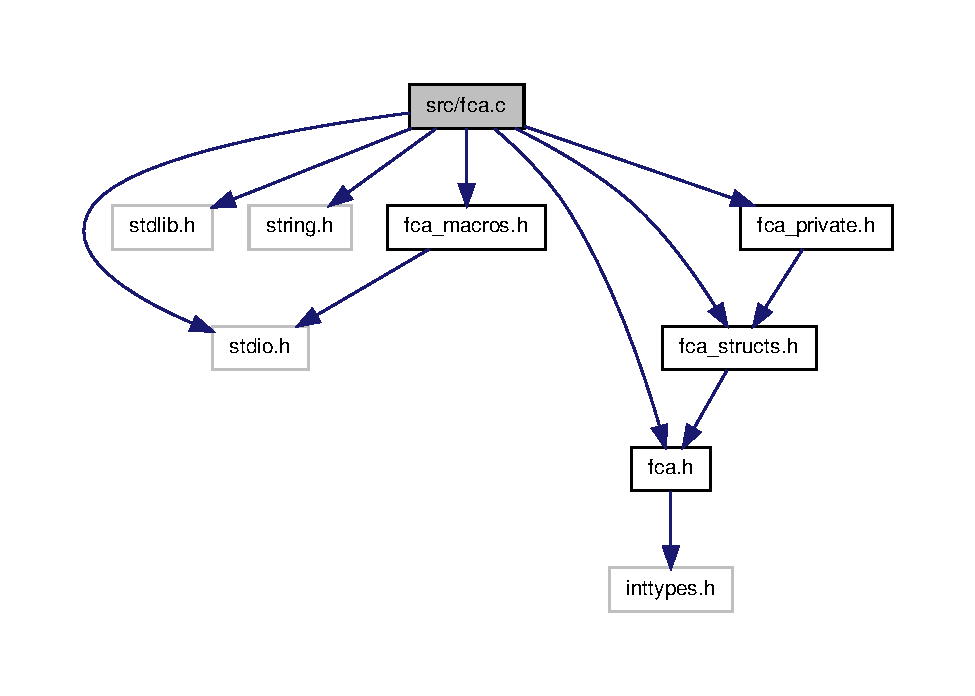
\includegraphics[width=350pt]{fca_8c__incl}
\end{center}
\end{figure}
\subsection*{\-Functions}
\begin{DoxyCompactItemize}
\item 
\hyperlink{fca_8h_ad53dc3fc96151a44387245e6481f95a4}{\-Formal\-Context} \hyperlink{fca_8c_a8cc0086fc3f45b783688b21105632456}{new\-Formal\-Context} (int objects, int attributes)
\begin{DoxyCompactList}\small\item\em create a new formal context \end{DoxyCompactList}\item 
\hyperlink{fca_8h_ad53dc3fc96151a44387245e6481f95a4}{\-Formal\-Context} \hyperlink{fca_8c_af3e05ebca016a7d4d09b332eac01a456}{new\-Formal\-Context\-From\-File} (const char $\ast$filename)
\begin{DoxyCompactList}\small\item\em create a new formal context object from a .cxt file \end{DoxyCompactList}\item 
void \hyperlink{fca_8c_a064800878bf96c6398d2f716609df081}{write\-Formal\-Context} (\hyperlink{fca_8h_ad53dc3fc96151a44387245e6481f95a4}{\-Formal\-Context} ctx, const char $\ast$filename)
\begin{DoxyCompactList}\small\item\em save the context ctx at the given file location \end{DoxyCompactList}\item 
void \hyperlink{fca_8c_a9835be78a56a9eaec5346a86562f10c3}{delete\-Formal\-Context} (\hyperlink{fca_8h_ad53dc3fc96151a44387245e6481f95a4}{\-Formal\-Context} $\ast$ctx)
\begin{DoxyCompactList}\small\item\em deletes the formal context $\ast$ctx, and sets the pointer to zero \end{DoxyCompactList}\item 
\hyperlink{easy_2structs_8h_ae552e1b13988c8c4ca0ab8f8a3e60f96}{my\-Formal\-Concept\-Intent\-Chunk} $\ast$ \hyperlink{fca_8c_a10016c73379236582a412ab83e159618}{new\-Concept\-Chunk} (int attributes)
\begin{DoxyCompactList}\small\item\em create a new formal concept chunk \end{DoxyCompactList}\item 
void \hyperlink{fca_8c_ad13aa7f16480d11c9c89310cca51670b}{delete\-Concept\-Chunk} (\hyperlink{easy_2structs_8h_ae552e1b13988c8c4ca0ab8f8a3e60f96}{my\-Formal\-Concept\-Intent\-Chunk} $\ast$$\ast$c)
\begin{DoxyCompactList}\small\item\em deletes a concept chunk object and sets its pointer to zero \end{DoxyCompactList}\item 
\hyperlink{easy_2structs_8h_a6c7fd90fd34d9ca52fedd96a01dd3566}{\-Formal\-Concept\-Intent\-Bulk\-List} \hyperlink{fca_8c_a709ef22f213a99f6a46ca8aa78328ece}{new\-Concept\-Bulk} (int attributes)
\begin{DoxyCompactList}\small\item\em creates a new formal concept intent bulk list \end{DoxyCompactList}\item 
void \hyperlink{fca_8c_acd989c02b03c2cc8bf2d477d2f5636e5}{delete\-Concept\-Bulk} (\hyperlink{easy_2structs_8h_a6c7fd90fd34d9ca52fedd96a01dd3566}{\-Formal\-Concept\-Intent\-Bulk\-List} $\ast$root\-Node)
\begin{DoxyCompactList}\small\item\em deletes the entire bulk list \end{DoxyCompactList}\item 
int \hyperlink{fca_8c_a965bdc1065d581495114a764020c3c6b}{count\-Concepts\-In\-Bulk} (\hyperlink{easy_2structs_8h_a6c7fd90fd34d9ca52fedd96a01dd3566}{\-Formal\-Concept\-Intent\-Bulk\-List} root)
\begin{DoxyCompactList}\small\item\em use this for bulks that are filled in order \end{DoxyCompactList}\item 
\hyperlink{easy_2structs_8h_a6c7fd90fd34d9ca52fedd96a01dd3566}{\-Formal\-Concept\-Intent\-Bulk\-List} \hyperlink{fca_8c_ac9e73d5390011291b92740d99f186ab4}{add\-Concept\-To\-Bulk} (\hyperlink{easy_2structs_8h_a6c7fd90fd34d9ca52fedd96a01dd3566}{\-Formal\-Concept\-Intent\-Bulk\-List} root, const \hyperlink{fca_8h_a92fa84ef7a12663bb998f141ab729056}{\-Incidence\-Cell} $\ast$intent)
\begin{DoxyCompactList}\small\item\em copies the given intent to the bulk denoted by the root node. \end{DoxyCompactList}\item 
void \hyperlink{fca_8c_a4596b3e7b389078cc2dab62448e0c58c}{close\-Intent2} (\hyperlink{fca_8h_ad53dc3fc96151a44387245e6481f95a4}{\-Formal\-Context} ctx, const \hyperlink{fca_8h_a92fa84ef7a12663bb998f141ab729056}{\-Incidence\-Cell} $\ast$input, \hyperlink{fca_8h_a92fa84ef7a12663bb998f141ab729056}{\-Incidence\-Cell} $\ast$output\-Intent, \hyperlink{fca_8h_a92fa84ef7a12663bb998f141ab729056}{\-Incidence\-Cell} $\ast$output\-Extent)
\begin{DoxyCompactList}\small\item\em close an attribute set, i.\-e. \end{DoxyCompactList}\item 
void \hyperlink{fca_8c_ae932250c17890745228ddb08bb856e40}{close\-Intent} (\hyperlink{fca_8h_ad53dc3fc96151a44387245e6481f95a4}{\-Formal\-Context} ctx, const \hyperlink{fca_8h_a92fa84ef7a12663bb998f141ab729056}{\-Incidence\-Cell} $\ast$input, \hyperlink{fca_8h_a92fa84ef7a12663bb998f141ab729056}{\-Incidence\-Cell} $\ast$output)
\begin{DoxyCompactList}\small\item\em close an attribute set, i.\-e. \end{DoxyCompactList}\item 
int \hyperlink{fca_8c_a3eff21bebd55849e1049f6d8b6c50a8b}{intent\-Cmp} (int attributes, const \hyperlink{fca_8h_a92fa84ef7a12663bb998f141ab729056}{\-Incidence\-Cell} $\ast$minus, const \hyperlink{fca_8h_a92fa84ef7a12663bb998f141ab729056}{\-Incidence\-Cell} $\ast$plus)
\begin{DoxyCompactList}\small\item\em compare two intent vectors \end{DoxyCompactList}\item 
\hyperlink{easy_2structs_8h_a6c7fd90fd34d9ca52fedd96a01dd3566}{\-Formal\-Concept\-Intent\-Bulk\-List} \hyperlink{fca_8c_a629cb24ff7d30d56d803e1848ff0019d}{new\-Concept\-Bulk\-From\-Context} (\hyperlink{fca_8h_ad53dc3fc96151a44387245e6481f95a4}{\-Formal\-Context} ctx)
\begin{DoxyCompactList}\small\item\em creates a new formal concept intent chunk and fills it with the intents of all formal concepts in the concept lattice of ctx, using next closure algorithm \end{DoxyCompactList}\item 
void \hyperlink{fca_8c_ac1a973138b558d99763bfa84d022d42d}{write\-Concepts\-To\-File} (\hyperlink{fca_8h_ad53dc3fc96151a44387245e6481f95a4}{\-Formal\-Context} ctx, \hyperlink{easy_2structs_8h_a6c7fd90fd34d9ca52fedd96a01dd3566}{\-Formal\-Concept\-Intent\-Bulk\-List} root, const char $\ast$filename)
\begin{DoxyCompactList}\small\item\em write a list of concept intents into a .cxt file \end{DoxyCompactList}\item 
\hyperlink{fca_8h_ad53dc3fc96151a44387245e6481f95a4}{\-Formal\-Context} \hyperlink{fca_8c_ae3105d9c1d91e1816c8b7a83d3414790}{new\-Formal\-Context\-From\-Random} (int objects, int attributes, float p)
\begin{DoxyCompactList}\small\item\em create a new formal context with random incidence relation \end{DoxyCompactList}\item 
int \hyperlink{fca_8c_ae4afb43074af0e6432681f3b4e733fc5}{count\-Context\-Concepts2} (\hyperlink{fca_8h_ad53dc3fc96151a44387245e6481f95a4}{\-Formal\-Context} ctx)
\begin{DoxyCompactList}\small\item\em counts the concepts in the concept lattice of ctx, using next closure algorithm \end{DoxyCompactList}\item 
int \hyperlink{fca_8c_aaf6da61c84352d127039536dd6e790b6}{count\-Context\-Concepts} (\hyperlink{fca_8h_ad53dc3fc96151a44387245e6481f95a4}{\-Formal\-Context} ctx)
\begin{DoxyCompactList}\small\item\em counts the concepts in the concept lattice of ctx, using next closure algorithm \end{DoxyCompactList}\end{DoxyCompactItemize}


\subsection{\-Detailed \-Description}
\hyperlink{fca_8c}{fca.\-c}, (c) 2013, \-Immanuel \-Albrecht; \-Dresden \-University of \-Technology, \-Professur für die \-Psychologie des \-Lernen und \-Lehrens \-This program is free software\-: you can redistribute it and/or modify it under the terms of the \-G\-N\-U \-General \-Public \-License as published by the \-Free \-Software \-Foundation, either version 3 of the \-License, or (at your option) any later version.

\-This program is distributed in the hope that it will be useful, but \-W\-I\-T\-H\-O\-U\-T \-A\-N\-Y \-W\-A\-R\-R\-A\-N\-T\-Y; without even the implied warranty of \-M\-E\-R\-C\-H\-A\-N\-T\-A\-B\-I\-L\-I\-T\-Y or \-F\-I\-T\-N\-E\-S\-S \-F\-O\-R \-A \-P\-A\-R\-T\-I\-C\-U\-L\-A\-R \-P\-U\-R\-P\-O\-S\-E. \-See the \-G\-N\-U \-General \-Public \-License for more details.

\-You should have received a copy of the \-G\-N\-U \-General \-Public \-License along with this program. \-If not, see $<$\href{http://www.gnu.org/licenses/}{\tt http\-://www.\-gnu.\-org/licenses/}$>$. this file contains general formal context related operations and routines 

\-Definition in file \hyperlink{fca_8c_source}{fca.\-c}.



\subsection{\-Function \-Documentation}
\hypertarget{fca_8c_ac9e73d5390011291b92740d99f186ab4}{\index{fca.\-c@{fca.\-c}!add\-Concept\-To\-Bulk@{add\-Concept\-To\-Bulk}}
\index{add\-Concept\-To\-Bulk@{add\-Concept\-To\-Bulk}!fca.c@{fca.\-c}}
\subsubsection[{add\-Concept\-To\-Bulk}]{\setlength{\rightskip}{0pt plus 5cm}{\bf \-Formal\-Concept\-Intent\-Bulk\-List} {\bf add\-Concept\-To\-Bulk} (
\begin{DoxyParamCaption}
\item[{{\bf \-Formal\-Concept\-Intent\-Bulk\-List}}]{root, }
\item[{const {\bf \-Incidence\-Cell} $\ast$}]{intent}
\end{DoxyParamCaption}
)}}\label{fca_8c_ac9e73d5390011291b92740d99f186ab4}


copies the given intent to the bulk denoted by the root node. 


\begin{DoxyParams}{\-Parameters}
{\em root} & root node of the bulk \\
\hline
{\em intent} & read-\/only pointer to an array of \-Incidence\-Cell\mbox{[}root-\/$>$attributes\mbox{]}\\
\hline
\end{DoxyParams}
\begin{DoxyReturn}{\-Returns}
the node where the intent was added to the last chunk 
\end{DoxyReturn}


\-Definition at line 427 of file fca.\-c.



\-References s\-Formal\-Concept\-Intent\-Bulk\-Node\-::attributes, \-B\-U\-L\-K\-S\-I\-Z\-E, \-C\-E\-L\-L, s\-Formal\-Concept\-Intent\-Bulk\-Node\-::chunks, \-C\-H\-U\-N\-K\-S\-I\-Z\-E, new\-Concept\-Bulk(), new\-Concept\-Chunk(), s\-Formal\-Concept\-Intent\-Bulk\-Node\-::next, \-R\-E\-T\-U\-R\-N\-\_\-\-Z\-E\-R\-O\-\_\-\-I\-F\-\_\-\-Z\-E\-R\-O, smy\-Formal\-Concept\-Intent\-Chunk\-::size, and s\-Formal\-Concept\-Intent\-Bulk\-Node\-::size.



\-Referenced by new\-Concept\-Bulk\-From\-Context().


\begin{DoxyCode}
{
    RETURN_ZERO_IF_ZERO(root);

    do
    {

        if (root->size == 0)
        {
            root->chunks[0] = newConceptChunk(root->attributes);
            root->size = 1;
        }

        int last_index;
        last_index = root->size - 1;

        if (root->chunks[last_index]->size == CHUNKSIZE)
        {
            if (root->size == BULKSIZE)
            {
                if (root->next == 0)
                {
                    root->next = newConceptBulk(root->attributes);
                }
                root = root->next;
                continue;
            }
            else
            {
                last_index = root->size++;
                root->chunks[last_index] = newConceptChunk(root->attributes);
            }
        }

#pragma GCC diagnostic push
#pragma GCC diagnostic ignored "-Wsign-conversion"

        memcpy(
                &(CELL(root->chunks[last_index]->size, root->chunks[last_index]
      ,0)),
                intent, sizeof(IncidenceCell) * root->attributes);

#pragma GCC diagnostic pop

        root->chunks[last_index]->size++;

        break;

    } while (1);

    return root;
}
\end{DoxyCode}


\-Here is the call graph for this function\-:\nopagebreak
\begin{figure}[H]
\begin{center}
\leavevmode
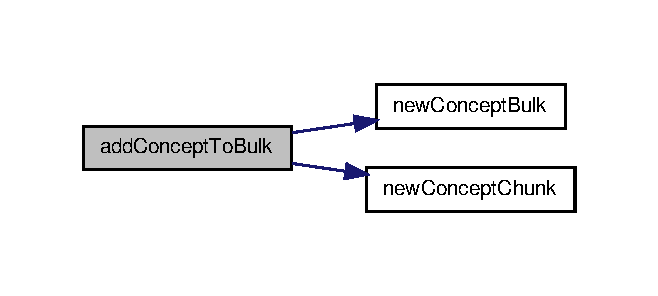
\includegraphics[width=316pt]{fca_8c_ac9e73d5390011291b92740d99f186ab4_cgraph}
\end{center}
\end{figure}


\hypertarget{fca_8c_ae932250c17890745228ddb08bb856e40}{\index{fca.\-c@{fca.\-c}!close\-Intent@{close\-Intent}}
\index{close\-Intent@{close\-Intent}!fca.c@{fca.\-c}}
\subsubsection[{close\-Intent}]{\setlength{\rightskip}{0pt plus 5cm}void {\bf close\-Intent} (
\begin{DoxyParamCaption}
\item[{{\bf \-Formal\-Context}}]{ctx, }
\item[{const {\bf \-Incidence\-Cell} $\ast$}]{input, }
\item[{{\bf \-Incidence\-Cell} $\ast$}]{output}
\end{DoxyParamCaption}
)}}\label{fca_8c_ae932250c17890745228ddb08bb856e40}


close an attribute set, i.\-e. 

add further attributes


\begin{DoxyParams}{\-Parameters}
{\em ctx} & formal context \\
\hline
{\em input} & the intent set that is to be closed \\
\hline
{\em output} & the closure intent'' wrt. ctx \\
\hline
\end{DoxyParams}


\-Definition at line 538 of file fca.\-c.



\-References smy\-Formal\-Context\-::attributes, \-C\-L\-E\-A\-R, \-C\-R\-O\-S\-S, g\-Im, \-I\-N\-C\-I\-D\-E\-S, and smy\-Formal\-Context\-::objects.



\-Referenced by count\-Context\-Concepts(), and new\-Concept\-Bulk\-From\-Context().


\begin{DoxyCode}
{

    myFormalContext* I;
    I = (myFormalContext*) ctx;
    for (int var = 0; var < I->attributes; ++var)
    {
        CROSS(output[var]);
    }

    for (int g = 0; g < I->objects; ++g)
    {
        int good;
        good = 1;

        for (int m = 0; m < I->attributes; ++m)
        {
            if (INCIDES(input[m]))
                if (!gIm(g,I,m))
                {
                    /*
                     * some attribute is not present for this object -> next
       object
                     */
                    good = 0;
                    break;
                }
        }
        if (good)
            /*
             * remove attributes that are not common among all objects that
       have the input
             * attributes
             */
            for (int m = 0; m < I->attributes; ++m)
            {
                if (!gIm(g,I,m))
                {
                    CLEAR(output[m]);
                }
            }
    }
}
\end{DoxyCode}
\hypertarget{fca_8c_a4596b3e7b389078cc2dab62448e0c58c}{\index{fca.\-c@{fca.\-c}!close\-Intent2@{close\-Intent2}}
\index{close\-Intent2@{close\-Intent2}!fca.c@{fca.\-c}}
\subsubsection[{close\-Intent2}]{\setlength{\rightskip}{0pt plus 5cm}void {\bf close\-Intent2} (
\begin{DoxyParamCaption}
\item[{{\bf \-Formal\-Context}}]{ctx, }
\item[{const {\bf \-Incidence\-Cell} $\ast$}]{input, }
\item[{{\bf \-Incidence\-Cell} $\ast$}]{output\-Intent, }
\item[{{\bf \-Incidence\-Cell} $\ast$}]{output\-Extent}
\end{DoxyParamCaption}
)}}\label{fca_8c_a4596b3e7b389078cc2dab62448e0c58c}


close an attribute set, i.\-e. 

add further attributes, 1.\-92 times slower than close\-Intent


\begin{DoxyParams}{\-Parameters}
{\em ctx} & formal context \\
\hline
{\em input} & the intent set that is to be closed \\
\hline
{\em output\-Intent} & the closure intent'' wrt. ctx \\
\hline
{\em output\-Extent} & the corresponding objects, i.\-e. intent' wrt. ctx \\
\hline
\end{DoxyParams}


\-Definition at line 491 of file fca.\-c.



\-References smy\-Formal\-Context\-::attributes, \-C\-L\-E\-A\-R, \-C\-R\-O\-S\-S, g\-Im, \-I\-N\-C\-I\-D\-E\-S, and smy\-Formal\-Context\-::objects.



\-Referenced by count\-Context\-Concepts2().


\begin{DoxyCode}
{
    myFormalContext* I;
    I = (myFormalContext*) ctx;

    for (int g = 0; g < I->objects; ++g)
    {
        CROSS(outputExtent[g]);
        for (int m = 0; m < I->attributes; ++m)
        {
            if (INCIDES(input[m]))
                if (!gIm(g,I,m))
                {
                    /*
                     * some attribute is not present for this object -> next
       object
                     */
                    CLEAR(outputExtent[g]);
                    break;
                }
        }
    }

    for (int m = 0; m < I->attributes; ++m)
    {
        CROSS(outputIntent[m]);
        for (int g = 0; g < I->objects; ++g)
        {
            if (INCIDES(outputExtent[g]))
                if (!gIm(g,I,m))
                {
                    CLEAR(outputIntent[m]);
                    break;
                }
        }
    }

}
\end{DoxyCode}
\hypertarget{fca_8c_a965bdc1065d581495114a764020c3c6b}{\index{fca.\-c@{fca.\-c}!count\-Concepts\-In\-Bulk@{count\-Concepts\-In\-Bulk}}
\index{count\-Concepts\-In\-Bulk@{count\-Concepts\-In\-Bulk}!fca.c@{fca.\-c}}
\subsubsection[{count\-Concepts\-In\-Bulk}]{\setlength{\rightskip}{0pt plus 5cm}int {\bf count\-Concepts\-In\-Bulk} (
\begin{DoxyParamCaption}
\item[{{\bf \-Formal\-Concept\-Intent\-Bulk\-List}}]{root}
\end{DoxyParamCaption}
)}}\label{fca_8c_a965bdc1065d581495114a764020c3c6b}


use this for bulks that are filled in order 


\begin{DoxyParams}{\-Parameters}
{\em root} & \\
\hline
\end{DoxyParams}
\begin{DoxyReturn}{\-Returns}
number of concepts in bulk 
\end{DoxyReturn}


\-Definition at line 392 of file fca.\-c.



\-References s\-Formal\-Concept\-Intent\-Bulk\-Node\-::chunks, \-C\-H\-U\-N\-K\-S\-I\-Z\-E, s\-Formal\-Concept\-Intent\-Bulk\-Node\-::next, \-R\-E\-T\-U\-R\-N\-\_\-\-Z\-E\-R\-O\-\_\-\-I\-F\-\_\-\-Z\-E\-R\-O, smy\-Formal\-Concept\-Intent\-Chunk\-::size, and s\-Formal\-Concept\-Intent\-Bulk\-Node\-::size.



\-Referenced by main(), and write\-Concepts\-To\-File().


\begin{DoxyCode}
{
    RETURN_ZERO_IF_ZERO(root);

    int count = 0;

    while (root != 0)
    {
        if (root->size > 0)
        {
            /*
             * count the full chunks
             */
            count += CHUNKSIZE * (root->size - 1);
            /*
             * and the last chunk
             */
            count += root->chunks[root->size - 1]->size;
        }
        root = root->next;
    }

    return count;
}
\end{DoxyCode}
\hypertarget{fca_8c_aaf6da61c84352d127039536dd6e790b6}{\index{fca.\-c@{fca.\-c}!count\-Context\-Concepts@{count\-Context\-Concepts}}
\index{count\-Context\-Concepts@{count\-Context\-Concepts}!fca.c@{fca.\-c}}
\subsubsection[{count\-Context\-Concepts}]{\setlength{\rightskip}{0pt plus 5cm}int {\bf count\-Context\-Concepts} (
\begin{DoxyParamCaption}
\item[{{\bf \-Formal\-Context}}]{ctx}
\end{DoxyParamCaption}
)}}\label{fca_8c_aaf6da61c84352d127039536dd6e790b6}


counts the concepts in the concept lattice of ctx, using next closure algorithm 


\begin{DoxyParams}{\-Parameters}
{\em ctx} & formal context \\
\hline
\end{DoxyParams}
\begin{DoxyReturn}{\-Returns}
number of concepts in context 
\end{DoxyReturn}


\-Definition at line 930 of file fca.\-c.



\-References smy\-Formal\-Context\-::attributes, \-C\-L\-E\-A\-R, close\-Intent(), \-C\-R\-O\-S\-S, \-I\-N\-C\-I\-D\-E\-S, and \-R\-E\-T\-U\-R\-N\-\_\-\-Z\-E\-R\-O\-\_\-\-I\-F\-\_\-\-Z\-E\-R\-O.


\begin{DoxyCode}
{
    RETURN_ZERO_IF_ZERO(ctx);

    myFormalContext *c;
    c = (myFormalContext*) ctx;

    IncidenceCell *M;
    IncidenceCell *Y;

#pragma GCC diagnostic push
#pragma GCC diagnostic ignored "-Wsign-conversion"

    Y = calloc(c->attributes, sizeof(IncidenceCell));
    M = malloc(c->attributes * sizeof(IncidenceCell));


#pragma GCC diagnostic pop

    /*
     * calculate the bottom intent of the concept lattice, i.e. {}''
     */
    closeIntent(ctx, Y, M);

    int count;

    count = 1;

    /*
     * begin of nextClosure function iteration
     */
    nextClosure:

    for (int i = c->attributes - 1; i >= 0; --i)
    {

        if (!INCIDES(M[i]))
        {
            CROSS(M[i]);
            closeIntent(ctx, M, Y);

            int good;
            good = 1;

            for (int j = 0; j < i; ++j)
            {
                if (INCIDES(Y[j]))
                {
                    if (!INCIDES((M[j])))
                    {

                        good = 0;
                        break;
                    }
                }
            }
            if (good)
            {
                /*
                 * we found the next intent
                 */
                count++;

                /*
                 * continue with Y for M
                 */

                IncidenceCell *DELTA;
                DELTA = M;
                M = Y;
                Y = DELTA;
                /*
                 * do the nextClosure
                 */
                goto nextClosure;
            }
        }

        CLEAR(M[i]);
    }

    /*
     * free up memory
     */

    free(M);
    free(Y);

    return count;
}
\end{DoxyCode}


\-Here is the call graph for this function\-:\nopagebreak
\begin{figure}[H]
\begin{center}
\leavevmode
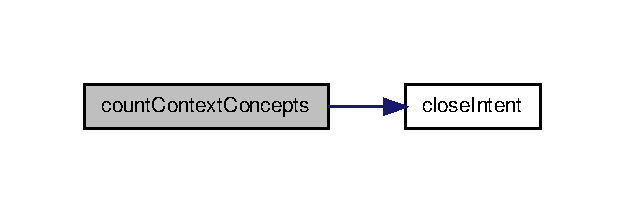
\includegraphics[width=300pt]{fca_8c_aaf6da61c84352d127039536dd6e790b6_cgraph}
\end{center}
\end{figure}


\hypertarget{fca_8c_ae4afb43074af0e6432681f3b4e733fc5}{\index{fca.\-c@{fca.\-c}!count\-Context\-Concepts2@{count\-Context\-Concepts2}}
\index{count\-Context\-Concepts2@{count\-Context\-Concepts2}!fca.c@{fca.\-c}}
\subsubsection[{count\-Context\-Concepts2}]{\setlength{\rightskip}{0pt plus 5cm}int {\bf count\-Context\-Concepts2} (
\begin{DoxyParamCaption}
\item[{{\bf \-Formal\-Context}}]{ctx}
\end{DoxyParamCaption}
)}}\label{fca_8c_ae4afb43074af0e6432681f3b4e733fc5}


counts the concepts in the concept lattice of ctx, using next closure algorithm 


\begin{DoxyParams}{\-Parameters}
{\em ctx} & formal context \\
\hline
\end{DoxyParams}
\begin{DoxyReturn}{\-Returns}
number of concepts in context 
\end{DoxyReturn}


\-Definition at line 832 of file fca.\-c.



\-References smy\-Formal\-Context\-::attributes, \-C\-L\-E\-A\-R, close\-Intent2(), \-C\-R\-O\-S\-S, \-I\-N\-C\-I\-D\-E\-S, smy\-Formal\-Context\-::objects, and \-R\-E\-T\-U\-R\-N\-\_\-\-Z\-E\-R\-O\-\_\-\-I\-F\-\_\-\-Z\-E\-R\-O.


\begin{DoxyCode}
{
    RETURN_ZERO_IF_ZERO(ctx);

    myFormalContext *c;
    c = (myFormalContext*) ctx;

    IncidenceCell *M;
    IncidenceCell *Y;
    IncidenceCell *extent;

#pragma GCC diagnostic push
#pragma GCC diagnostic ignored "-Wsign-conversion"

    Y = calloc(c->attributes, sizeof(IncidenceCell));
    M = malloc(c->attributes * sizeof(IncidenceCell));
    extent = malloc(c->objects * sizeof(IncidenceCell));

#pragma GCC diagnostic pop

    /*
     * calculate the bottom intent of the concept lattice, i.e. {}''
     */
    closeIntent2(ctx, Y, M, extent);

    int count;

    count = 1;

    /*
     * begin of nextClosure function iteration
     */
    nextClosure:

    for (int i = c->attributes - 1; i >= 0; --i)
    {

        if (!INCIDES(M[i]))
        {
            CROSS(M[i]);
            closeIntent2(ctx, M, Y, extent);

            int good;
            good = 1;

            for (int j = 0; j < i; ++j)
            {
                if (INCIDES(Y[j]))
                {
                    if (!INCIDES((M[j])))
                    {

                        good = 0;
                        break;
                    }
                }
            }
            if (good)
            {
                /*
                 * we found the next intent
                 */
                count++;

                /*
                 * continue with Y for M
                 */

                IncidenceCell *DELTA;
                DELTA = M;
                M = Y;
                Y = DELTA;
                /*
                 * do the nextClosure
                 */
                goto nextClosure;
            }
        }

        CLEAR(M[i]);
    }

    /*
     * free up memory
     */

    free(M);
    free(Y);
    free(extent);
    return count;
}
\end{DoxyCode}


\-Here is the call graph for this function\-:\nopagebreak
\begin{figure}[H]
\begin{center}
\leavevmode
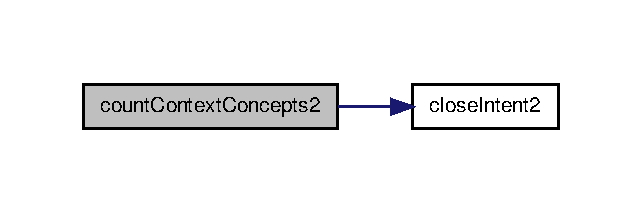
\includegraphics[width=308pt]{fca_8c_ae4afb43074af0e6432681f3b4e733fc5_cgraph}
\end{center}
\end{figure}


\hypertarget{fca_8c_acd989c02b03c2cc8bf2d477d2f5636e5}{\index{fca.\-c@{fca.\-c}!delete\-Concept\-Bulk@{delete\-Concept\-Bulk}}
\index{delete\-Concept\-Bulk@{delete\-Concept\-Bulk}!fca.c@{fca.\-c}}
\subsubsection[{delete\-Concept\-Bulk}]{\setlength{\rightskip}{0pt plus 5cm}void {\bf delete\-Concept\-Bulk} (
\begin{DoxyParamCaption}
\item[{{\bf \-Formal\-Concept\-Intent\-Bulk\-List} $\ast$}]{root\-Node}
\end{DoxyParamCaption}
)}}\label{fca_8c_acd989c02b03c2cc8bf2d477d2f5636e5}


deletes the entire bulk list 


\begin{DoxyParams}{\-Parameters}
{\em root\-Node} & pointer to the first node \\
\hline
\end{DoxyParams}


\-Definition at line 360 of file fca.\-c.



\-References s\-Formal\-Concept\-Intent\-Bulk\-Node\-::chunks, delete\-Concept\-Chunk(), s\-Formal\-Concept\-Intent\-Bulk\-Node\-::next, \-R\-E\-T\-U\-R\-N\-\_\-\-I\-F\-\_\-\-Z\-E\-R\-O, and s\-Formal\-Concept\-Intent\-Bulk\-Node\-::size.



\-Referenced by main().


\begin{DoxyCode}
{
    RETURN_IF_ZERO(rootNode);
    RETURN_IF_ZERO(*rootNode);

    FormalConceptIntentBulkList l;
    l = *rootNode;
    *rootNode = 0;

    do
    {
        for (int var = 0; var < l->size; ++var)
        {
            deleteConceptChunk(&(l->chunks[var]));
        }

        FormalConceptIntentBulkList next;
        next = l->next;

        free(l->chunks);
        free(l);

        l = next;
    } while (l != 0);
}
\end{DoxyCode}


\-Here is the call graph for this function\-:\nopagebreak
\begin{figure}[H]
\begin{center}
\leavevmode
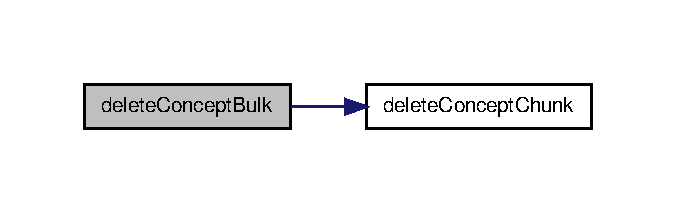
\includegraphics[width=324pt]{fca_8c_acd989c02b03c2cc8bf2d477d2f5636e5_cgraph}
\end{center}
\end{figure}


\hypertarget{fca_8c_ad13aa7f16480d11c9c89310cca51670b}{\index{fca.\-c@{fca.\-c}!delete\-Concept\-Chunk@{delete\-Concept\-Chunk}}
\index{delete\-Concept\-Chunk@{delete\-Concept\-Chunk}!fca.c@{fca.\-c}}
\subsubsection[{delete\-Concept\-Chunk}]{\setlength{\rightskip}{0pt plus 5cm}void {\bf delete\-Concept\-Chunk} (
\begin{DoxyParamCaption}
\item[{{\bf my\-Formal\-Concept\-Intent\-Chunk} $\ast$$\ast$}]{c}
\end{DoxyParamCaption}
)}}\label{fca_8c_ad13aa7f16480d11c9c89310cca51670b}


deletes a concept chunk object and sets its pointer to zero 


\begin{DoxyParams}{\-Parameters}
{\em c} & pointer to the concept chunk to be deleted \\
\hline
\end{DoxyParams}


\-Definition at line 325 of file fca.\-c.



\-References \-R\-E\-T\-U\-R\-N\-\_\-\-I\-F\-\_\-\-Z\-E\-R\-O.



\-Referenced by delete\-Concept\-Bulk().


\begin{DoxyCode}
{
    RETURN_IF_ZERO(c);
    RETURN_IF_ZERO(*c);

    free((*c)->incidence);

    free(*c);
    *c = 0;
}
\end{DoxyCode}
\hypertarget{fca_8c_a9835be78a56a9eaec5346a86562f10c3}{\index{fca.\-c@{fca.\-c}!delete\-Formal\-Context@{delete\-Formal\-Context}}
\index{delete\-Formal\-Context@{delete\-Formal\-Context}!fca.c@{fca.\-c}}
\subsubsection[{delete\-Formal\-Context}]{\setlength{\rightskip}{0pt plus 5cm}void {\bf delete\-Formal\-Context} (
\begin{DoxyParamCaption}
\item[{{\bf \-Formal\-Context} $\ast$}]{ctx}
\end{DoxyParamCaption}
)}}\label{fca_8c_a9835be78a56a9eaec5346a86562f10c3}


deletes the formal context $\ast$ctx, and sets the pointer to zero 


\begin{DoxyParams}{\-Parameters}
{\em ctx} & pointer to the formal context object to be deleted \\
\hline
\end{DoxyParams}


\-Definition at line 268 of file fca.\-c.



\-References smy\-Formal\-Context\-::attribute\-Names, smy\-Formal\-Context\-::attributes, smy\-Formal\-Context\-::incidence, smy\-Formal\-Context\-::object\-Names, smy\-Formal\-Context\-::objects, and \-R\-E\-T\-U\-R\-N\-\_\-\-I\-F\-\_\-\-Z\-E\-R\-O.



\-Referenced by main().


\begin{DoxyCode}
{
    RETURN_IF_ZERO(ctx);
    RETURN_IF_ZERO(*ctx);

    myFormalContext *c;

    c = (myFormalContext*) *ctx;

    *ctx = 0;

    for (int var = 0; var < c->attributes; ++var)
    {
        free(c->attributeNames[var]);
    }

    for (int var = 0; var < c->objects; ++var)
    {
        free(c->objectNames[var]);
    }

    free(c->objectNames);
    free(c->attributeNames);
    free(c->incidence);
    free(c);
}
\end{DoxyCode}
\hypertarget{fca_8c_a3eff21bebd55849e1049f6d8b6c50a8b}{\index{fca.\-c@{fca.\-c}!intent\-Cmp@{intent\-Cmp}}
\index{intent\-Cmp@{intent\-Cmp}!fca.c@{fca.\-c}}
\subsubsection[{intent\-Cmp}]{\setlength{\rightskip}{0pt plus 5cm}int {\bf intent\-Cmp} (
\begin{DoxyParamCaption}
\item[{int}]{attributes, }
\item[{const {\bf \-Incidence\-Cell} $\ast$}]{minus, }
\item[{const {\bf \-Incidence\-Cell} $\ast$}]{plus}
\end{DoxyParamCaption}
)}}\label{fca_8c_a3eff21bebd55849e1049f6d8b6c50a8b}


compare two intent vectors 


\begin{DoxyParams}{\-Parameters}
{\em attributes} & attribute count \\
\hline
{\em minus} & \char`\"{}left\char`\"{} operand \\
\hline
{\em plus} & \char`\"{}right\char`\"{} operand \\
\hline
\end{DoxyParams}
\begin{DoxyReturn}{\-Returns}
-\/1 if minus is bigger, 1 if plus is bigger, 0 if minus and plus is the same 
\end{DoxyReturn}


\-Definition at line 591 of file fca.\-c.



\-References \-I\-N\-C\-I\-D\-E\-S.


\begin{DoxyCode}
{
    for (int var = 0; var < attributes; ++var)
    {
        if (INCIDES(minus[var]))
        {
            if (!INCIDES((plus[var])))
                return -1;
        }
        else if (INCIDES(plus[var]))
        {
            return 1;
        }
    }
    return 0;
}
\end{DoxyCode}
\hypertarget{fca_8c_a709ef22f213a99f6a46ca8aa78328ece}{\index{fca.\-c@{fca.\-c}!new\-Concept\-Bulk@{new\-Concept\-Bulk}}
\index{new\-Concept\-Bulk@{new\-Concept\-Bulk}!fca.c@{fca.\-c}}
\subsubsection[{new\-Concept\-Bulk}]{\setlength{\rightskip}{0pt plus 5cm}{\bf \-Formal\-Concept\-Intent\-Bulk\-List} {\bf new\-Concept\-Bulk} (
\begin{DoxyParamCaption}
\item[{int}]{attributes}
\end{DoxyParamCaption}
)}}\label{fca_8c_a709ef22f213a99f6a46ca8aa78328ece}


creates a new formal concept intent bulk list 


\begin{DoxyParams}{\-Parameters}
{\em attributes} & number of attributes of the concept intents \\
\hline
\end{DoxyParams}
\begin{DoxyReturn}{\-Returns}
new formal concept intent bulk list's first node 
\end{DoxyReturn}


\-Definition at line 343 of file fca.\-c.



\-References s\-Formal\-Concept\-Intent\-Bulk\-Node\-::attributes, \-B\-U\-L\-K\-S\-I\-Z\-E, s\-Formal\-Concept\-Intent\-Bulk\-Node\-::chunks, s\-Formal\-Concept\-Intent\-Bulk\-Node\-::next, and s\-Formal\-Concept\-Intent\-Bulk\-Node\-::size.



\-Referenced by add\-Concept\-To\-Bulk(), and new\-Concept\-Bulk\-From\-Context().


\begin{DoxyCode}
{
    FormalConceptIntentBulkList l;
    l = malloc(sizeof(struct sFormalConceptIntentBulkNode));

    l->attributes = attributes;
    l->size = 0;
    l->chunks = calloc(BULKSIZE, sizeof(myFormalConceptIntentChunk*));
    l->next = 0;
    return l;
}
\end{DoxyCode}
\hypertarget{fca_8c_a629cb24ff7d30d56d803e1848ff0019d}{\index{fca.\-c@{fca.\-c}!new\-Concept\-Bulk\-From\-Context@{new\-Concept\-Bulk\-From\-Context}}
\index{new\-Concept\-Bulk\-From\-Context@{new\-Concept\-Bulk\-From\-Context}!fca.c@{fca.\-c}}
\subsubsection[{new\-Concept\-Bulk\-From\-Context}]{\setlength{\rightskip}{0pt plus 5cm}{\bf \-Formal\-Concept\-Intent\-Bulk\-List} {\bf new\-Concept\-Bulk\-From\-Context} (
\begin{DoxyParamCaption}
\item[{{\bf \-Formal\-Context}}]{ctx}
\end{DoxyParamCaption}
)}}\label{fca_8c_a629cb24ff7d30d56d803e1848ff0019d}


creates a new formal concept intent chunk and fills it with the intents of all formal concepts in the concept lattice of ctx, using next closure algorithm 


\begin{DoxyParams}{\-Parameters}
{\em ctx} & formal context \\
\hline
\end{DoxyParams}
\begin{DoxyReturn}{\-Returns}
concept intents 
\end{DoxyReturn}


\-Definition at line 616 of file fca.\-c.



\-References add\-Concept\-To\-Bulk(), smy\-Formal\-Context\-::attributes, \-C\-L\-E\-A\-R, close\-Intent(), \-C\-R\-O\-S\-S, \-I\-N\-C\-I\-D\-E\-S, new\-Concept\-Bulk(), and \-R\-E\-T\-U\-R\-N\-\_\-\-Z\-E\-R\-O\-\_\-\-I\-F\-\_\-\-Z\-E\-R\-O.



\-Referenced by main().


\begin{DoxyCode}
{
    RETURN_ZERO_IF_ZERO(ctx);

    myFormalContext *c;
    c = (myFormalContext*) ctx;

    IncidenceCell *M;
    IncidenceCell *Y;

#pragma GCC diagnostic push
#pragma GCC diagnostic ignored "-Wsign-conversion"

    Y = calloc(c->attributes, sizeof(IncidenceCell));
    M = malloc(c->attributes * sizeof(IncidenceCell));

#pragma GCC diagnostic pop

    /*
     * calculate the bottom intent of the concept lattice, i.e. {}''
     */
    closeIntent(ctx, Y, M);

    FormalConceptIntentBulkList root;
    FormalConceptIntentBulkList last;

    root = newConceptBulk(c->attributes);

    /*
     * add the bottom element of the concept lattice (a concept lattice is
       never empty)
     */

    last = addConceptToBulk(root, M);

    /*
     * begin of nextClosure function iteration
     */
    nextClosure:

    for (int i = c->attributes - 1; i >= 0; --i)
    {

        if (!INCIDES(M[i]))
        {
            CROSS(M[i]);
            closeIntent(ctx, M, Y);

            int good;
            good = 1;

            for (int j = 0; j < i; ++j)
            {
                if (INCIDES(Y[j]))
                {
                    if (!INCIDES((M[j])))
                    {

                        good = 0;
                        break;
                    }
                }
            }
            if (good)
            {
                /*
                 * we found the next intent
                 */
                last = addConceptToBulk(last, Y);

                /*
                 * continue with Y for M
                 */

                IncidenceCell *DELTA;
                DELTA = M;
                M = Y;
                Y = DELTA;
                /*
                 * do the nextClosure
                 */
                goto nextClosure;
            }
        }

        CLEAR(M[i]);
    }

    /*
     * free up memory
     */

    free(M);
    free(Y);
    return root;
}
\end{DoxyCode}


\-Here is the call graph for this function\-:\nopagebreak
\begin{figure}[H]
\begin{center}
\leavevmode
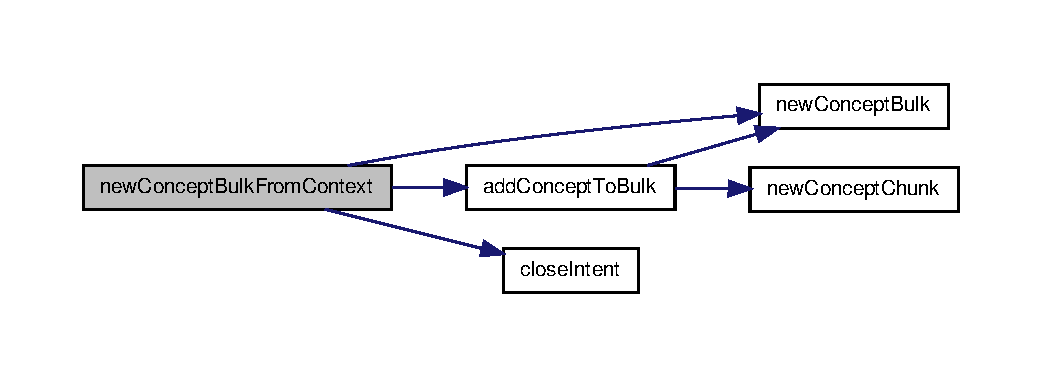
\includegraphics[width=350pt]{fca_8c_a629cb24ff7d30d56d803e1848ff0019d_cgraph}
\end{center}
\end{figure}


\hypertarget{fca_8c_a10016c73379236582a412ab83e159618}{\index{fca.\-c@{fca.\-c}!new\-Concept\-Chunk@{new\-Concept\-Chunk}}
\index{new\-Concept\-Chunk@{new\-Concept\-Chunk}!fca.c@{fca.\-c}}
\subsubsection[{new\-Concept\-Chunk}]{\setlength{\rightskip}{0pt plus 5cm}{\bf my\-Formal\-Concept\-Intent\-Chunk}$\ast$ {\bf new\-Concept\-Chunk} (
\begin{DoxyParamCaption}
\item[{int}]{attributes}
\end{DoxyParamCaption}
)}}\label{fca_8c_a10016c73379236582a412ab83e159618}


create a new formal concept chunk 

\hyperlink{easy_2private_8h}{easy/private.\-h}, (c) 2013, \-Immanuel \-Albrecht; \-Dresden \-University of \-Technology, \-Professur für die \-Psychologie des \-Lernen und \-Lehrens


\begin{DoxyParams}{\-Parameters}
{\em attributes} & number of attributes of the hosting formal context \\
\hline
\end{DoxyParams}
\begin{DoxyReturn}{\-Returns}
a new concept chunk object 
\end{DoxyReturn}


\-Definition at line 302 of file fca.\-c.



\-References smy\-Formal\-Concept\-Intent\-Chunk\-::attributes, \-C\-H\-U\-N\-K\-S\-I\-Z\-E, smy\-Formal\-Concept\-Intent\-Chunk\-::incidence, and smy\-Formal\-Concept\-Intent\-Chunk\-::size.



\-Referenced by add\-Concept\-To\-Bulk().


\begin{DoxyCode}
{
    myFormalConceptIntentChunk *c;
    c = malloc(sizeof(myFormalConceptIntentChunk));
    c->attributes = attributes;
    c->size = 0;

#pragma GCC diagnostic push
#pragma GCC diagnostic ignored "-Wsign-conversion"

    c->incidence = calloc(attributes * CHUNKSIZE, sizeof(IncidenceCell));

#pragma GCC diagnostic pop

    return c;
}
\end{DoxyCode}
\hypertarget{fca_8c_a8cc0086fc3f45b783688b21105632456}{\index{fca.\-c@{fca.\-c}!new\-Formal\-Context@{new\-Formal\-Context}}
\index{new\-Formal\-Context@{new\-Formal\-Context}!fca.c@{fca.\-c}}
\subsubsection[{new\-Formal\-Context}]{\setlength{\rightskip}{0pt plus 5cm}{\bf \-Formal\-Context} {\bf new\-Formal\-Context} (
\begin{DoxyParamCaption}
\item[{int}]{objects, }
\item[{int}]{attributes}
\end{DoxyParamCaption}
)}}\label{fca_8c_a8cc0086fc3f45b783688b21105632456}


create a new formal context 


\begin{DoxyParams}{\-Parameters}
{\em objects} & object count \\
\hline
{\em attributes} & attribute count \\
\hline
\end{DoxyParams}
\begin{DoxyReturn}{\-Returns}
a new \-Formal\-Context object 
\end{DoxyReturn}


\-Definition at line 42 of file fca.\-c.



\-References smy\-Formal\-Context\-::attribute\-Names, smy\-Formal\-Context\-::attributes, smy\-Formal\-Context\-::incidence, smy\-Formal\-Context\-::object\-Names, and smy\-Formal\-Context\-::objects.



\-Referenced by new\-Formal\-Context\-From\-File(), and new\-Formal\-Context\-From\-Random().


\begin{DoxyCode}
{
    myFormalContext *ctx = malloc(sizeof(myFormalContext));

    ctx->attributes = attributes;
    ctx->objects = objects;

#pragma GCC diagnostic push
#pragma GCC diagnostic ignored "-Wsign-conversion"

    ctx->attributeNames = calloc(attributes, sizeof(char*));
    ctx->objectNames = calloc(objects, sizeof(char*));

#pragma GCC diagnostic pop

    for (int var = 0; var < attributes; ++var)
    {
        ctx->attributeNames[var] = calloc(1, sizeof(char));
    }

    for (int var = 0; var < objects; ++var)
    {
        ctx->objectNames[var] = calloc(1, sizeof(char));
    }

#pragma GCC diagnostic push
#pragma GCC diagnostic ignored "-Wsign-conversion"

    ctx->incidence = calloc(objects * attributes, sizeof(IncidenceCell));

#pragma GCC diagnostic pop

    return (FormalContext) ctx;
}
\end{DoxyCode}
\hypertarget{fca_8c_af3e05ebca016a7d4d09b332eac01a456}{\index{fca.\-c@{fca.\-c}!new\-Formal\-Context\-From\-File@{new\-Formal\-Context\-From\-File}}
\index{new\-Formal\-Context\-From\-File@{new\-Formal\-Context\-From\-File}!fca.c@{fca.\-c}}
\subsubsection[{new\-Formal\-Context\-From\-File}]{\setlength{\rightskip}{0pt plus 5cm}{\bf \-Formal\-Context} {\bf new\-Formal\-Context\-From\-File} (
\begin{DoxyParamCaption}
\item[{const char $\ast$}]{filename}
\end{DoxyParamCaption}
)}}\label{fca_8c_af3e05ebca016a7d4d09b332eac01a456}


create a new formal context object from a .cxt file 


\begin{DoxyParams}{\-Parameters}
{\em filename} & \\
\hline
\end{DoxyParams}
\begin{DoxyReturn}{\-Returns}
the formal context that has been read from the given file 
\end{DoxyReturn}


\-Definition at line 84 of file fca.\-c.



\-References smy\-Formal\-Context\-::attribute\-Names, \-C\-E\-L\-L, \-C\-R\-O\-S\-S, \-I\-N\-P\-U\-T\-B\-U\-F\-F\-E\-R\-S\-I\-Z\-E, \-M\-I\-N, new\-Formal\-Context(), smy\-Formal\-Context\-::object\-Names, and \-R\-E\-T\-U\-R\-N\-\_\-\-Z\-E\-R\-O\-\_\-\-I\-F\-\_\-\-Z\-E\-R\-O.


\begin{DoxyCode}
{
    char *line;
    size_t len;

    len = (INPUTBUFFERSIZE);
    line = malloc(sizeof(char) * len);

    FILE *file;

    if (strcmp(filename, "-") == 0)
    {
        file = stdin;
    }
    else
    {
        file = fopen(filename, "r");
        RETURN_ZERO_IF_ZERO(file);
    }

    ssize_t read;

    int line_nbr;
    line_nbr = 0;

    int objects;
    int attributes;

    attributes = 0;
    objects = 0;

    myFormalContext *ctx;
    ctx = 0;

    while ((read = getline(&line, &len, file)) != -1)
    {

        /*
         * this should never happen, right?
         */
        if (read == 0)
            break;
        line[read - 1] = 0;

        if (line_nbr == 0)
        {
            if (strcmp(line, "B"))
            {
                fprintf(stderr, "File '%s' is not a .cxt file\n", filename);
                goto grace;
            }
        }
        else if (line_nbr == 1)
        {
            //empty line
        }
        else if (line_nbr == 2)
        {
            objects = atoi(line);
        }
        else if (line_nbr == 3)
        {
            attributes = atoi(line);
            ctx = (myFormalContext *) newFormalContext(objects, attributes);
        }
        else if (line_nbr == 4)
        {
            //empty line
        }
        else if (line_nbr < objects + 5)
        {

            int i;
            i = line_nbr - 5;

            free(ctx->objectNames[i]);
            ctx->objectNames[i] = strdup(line);

        }
        else if (line_nbr < objects + attributes + 5)
        {
            int i;
            i = line_nbr - 5 - objects;

            free(ctx->attributeNames[i]);
            ctx->attributeNames[i] = strdup(line);
        }
        else if (line_nbr < objects * 2 + attributes + 5)
        {
            int i;
            i = line_nbr - 5 - objects - attributes;

            int width;
            width = MIN((signed)strlen(line),attributes);

            for (int var = 0; var < width; ++var)
            {
                if ((line[var] == 'x') || (line[var] == 'X')
                        || (line[var] == '1'))
                {
                    CROSS(CELL (i, ctx, var));
                }
            }

        }
        else
        {
            /*
             * we read all data
             */
            break;
        }

        line_nbr++;
    }

    /*
     * free memory and return
     */

    grace: if (file != stdin)
    {
        fclose(file);
    }

    free(line);

    return (FormalContext) ctx;
}
\end{DoxyCode}


\-Here is the call graph for this function\-:\nopagebreak
\begin{figure}[H]
\begin{center}
\leavevmode
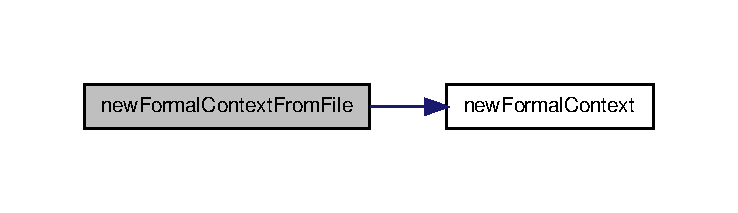
\includegraphics[width=350pt]{fca_8c_af3e05ebca016a7d4d09b332eac01a456_cgraph}
\end{center}
\end{figure}


\hypertarget{fca_8c_ae3105d9c1d91e1816c8b7a83d3414790}{\index{fca.\-c@{fca.\-c}!new\-Formal\-Context\-From\-Random@{new\-Formal\-Context\-From\-Random}}
\index{new\-Formal\-Context\-From\-Random@{new\-Formal\-Context\-From\-Random}!fca.c@{fca.\-c}}
\subsubsection[{new\-Formal\-Context\-From\-Random}]{\setlength{\rightskip}{0pt plus 5cm}{\bf \-Formal\-Context} {\bf new\-Formal\-Context\-From\-Random} (
\begin{DoxyParamCaption}
\item[{int}]{objects, }
\item[{int}]{attributes, }
\item[{float}]{p}
\end{DoxyParamCaption}
)}}\label{fca_8c_ae3105d9c1d91e1816c8b7a83d3414790}


create a new formal context with random incidence relation 


\begin{DoxyParams}{\-Parameters}
{\em objects} & \\
\hline
{\em attributes} & \\
\hline
{\em p} & probability of a cross \\
\hline
\end{DoxyParams}
\begin{DoxyReturn}{\-Returns}
context 
\end{DoxyReturn}


\-Definition at line 802 of file fca.\-c.



\-References smy\-Formal\-Context\-::attributes, \-C\-E\-L\-L, \-C\-R\-O\-S\-S, new\-Formal\-Context(), and smy\-Formal\-Context\-::objects.



\-Referenced by main().


\begin{DoxyCode}
{
    FormalContext ctx;
    ctx = newFormalContext(objects, attributes);

    myFormalContext *c;

    c = (myFormalContext*) ctx;

    for (int g = 0; g < c->objects; ++g)
    {
        for (int m = 0; m < c->attributes; ++m)
        {
            float x;
            x = (float) random() / (float) RAND_MAX;
            if (x >= p)
            {
                CROSS(CELL(g,c,m));
            }
        }
    }
    return ctx;
}
\end{DoxyCode}


\-Here is the call graph for this function\-:\nopagebreak
\begin{figure}[H]
\begin{center}
\leavevmode
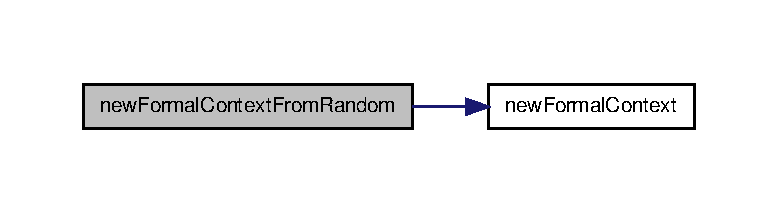
\includegraphics[width=350pt]{fca_8c_ae3105d9c1d91e1816c8b7a83d3414790_cgraph}
\end{center}
\end{figure}


\hypertarget{fca_8c_ac1a973138b558d99763bfa84d022d42d}{\index{fca.\-c@{fca.\-c}!write\-Concepts\-To\-File@{write\-Concepts\-To\-File}}
\index{write\-Concepts\-To\-File@{write\-Concepts\-To\-File}!fca.c@{fca.\-c}}
\subsubsection[{write\-Concepts\-To\-File}]{\setlength{\rightskip}{0pt plus 5cm}void {\bf write\-Concepts\-To\-File} (
\begin{DoxyParamCaption}
\item[{{\bf \-Formal\-Context}}]{ctx, }
\item[{{\bf \-Formal\-Concept\-Intent\-Bulk\-List}}]{root, }
\item[{const char $\ast$}]{filename}
\end{DoxyParamCaption}
)}}\label{fca_8c_ac1a973138b558d99763bfa84d022d42d}


write a list of concept intents into a .cxt file 


\begin{DoxyParams}{\-Parameters}
{\em ctx} & formal context (or 0, is used for attribute names) \\
\hline
{\em root} & the first node of the formal concept intent bulk \\
\hline
{\em filename} & output file name (.cxt) \\
\hline
\end{DoxyParams}


\-Definition at line 720 of file fca.\-c.



\-References smy\-Formal\-Context\-::attribute\-Names, smy\-Formal\-Context\-::attributes, s\-Formal\-Concept\-Intent\-Bulk\-Node\-::attributes, s\-Formal\-Concept\-Intent\-Bulk\-Node\-::chunks, count\-Concepts\-In\-Bulk(), g\-Im, s\-Formal\-Concept\-Intent\-Bulk\-Node\-::next, \-R\-E\-T\-U\-R\-N\-\_\-\-I\-F\-\_\-\-Z\-E\-R\-O, smy\-Formal\-Concept\-Intent\-Chunk\-::size, s\-Formal\-Concept\-Intent\-Bulk\-Node\-::size, and \-W\-A\-R\-N\-\_\-\-I\-F\-\_\-\-U\-N\-E\-Q\-U\-A\-L\-\_\-\-D\-O.



\-Referenced by main().


\begin{DoxyCode}
{
    RETURN_IF_ZERO(root);

    myFormalContext* c;

    if (ctx != 0)
    {
        c = (myFormalContext*) ctx;

        WARN_IF_UNEQUAL_DO(c->attributes, root->attributes, c = 0);
    }
    else
    {
        c = 0;
    }

    RETURN_IF_ZERO(filename);

    FILE* file;
    file = fopen(filename, "w");

    RETURN_IF_ZERO(file);

    int objects;
    objects = countConceptsInBulk(root);

    fprintf(file, "B\n\n%d\n%d\n\n", objects, root->attributes);

    for (int var = 0; var < objects; ++var)
    {
        fprintf(file, "C%8d\n", (var + 1));
    }

    if (c != 0)
    {
        for (int var = 0; var < c->attributes; ++var)
        {
            fputs(c->attributeNames[var], file);
            fputs("\n", file);
        }
    }
    else
    {
        for (int var = 0; var < root->attributes; ++var)
        {
            fprintf(file, "m%8d\n", (var + 1));
        }
    }

    for (; root != 0; root = root->next)
    {
        for (int chunk = 0; chunk < root->size; ++chunk)
        {
            for (int g = 0; g < root->chunks[chunk]->size; ++g)
            {
                for (int m = 0; m < root->attributes; ++m)
                {
                    if ( gIm(g, root->chunks[chunk], m))
                        fputs("X", file);
                    else
                        fputs(".", file);
                }
                fputs("\n", file);
            }
        }
    }

    fclose(file);

}
\end{DoxyCode}


\-Here is the call graph for this function\-:\nopagebreak
\begin{figure}[H]
\begin{center}
\leavevmode
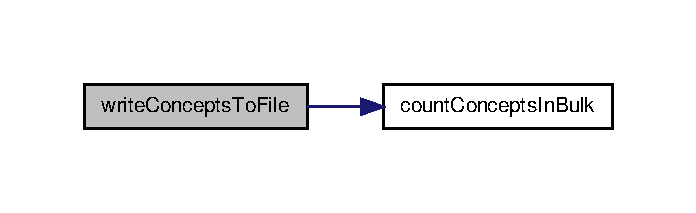
\includegraphics[width=334pt]{fca_8c_ac1a973138b558d99763bfa84d022d42d_cgraph}
\end{center}
\end{figure}


\hypertarget{fca_8c_a064800878bf96c6398d2f716609df081}{\index{fca.\-c@{fca.\-c}!write\-Formal\-Context@{write\-Formal\-Context}}
\index{write\-Formal\-Context@{write\-Formal\-Context}!fca.c@{fca.\-c}}
\subsubsection[{write\-Formal\-Context}]{\setlength{\rightskip}{0pt plus 5cm}void {\bf write\-Formal\-Context} (
\begin{DoxyParamCaption}
\item[{{\bf \-Formal\-Context}}]{ctx, }
\item[{const char $\ast$}]{filename}
\end{DoxyParamCaption}
)}}\label{fca_8c_a064800878bf96c6398d2f716609df081}


save the context ctx at the given file location 


\begin{DoxyParams}{\-Parameters}
{\em ctx} & \\
\hline
{\em filename} & \\
\hline
\end{DoxyParams}


\-Definition at line 220 of file fca.\-c.



\-References smy\-Formal\-Context\-::attribute\-Names, smy\-Formal\-Context\-::attributes, g\-Im, smy\-Formal\-Context\-::object\-Names, smy\-Formal\-Context\-::objects, and \-R\-E\-T\-U\-R\-N\-\_\-\-I\-F\-\_\-\-Z\-E\-R\-O.



\-Referenced by main().


\begin{DoxyCode}
{
    RETURN_IF_ZERO(ctx);
    RETURN_IF_ZERO(filename);

    FILE* file;
    file = fopen(filename, "w");

    RETURN_IF_ZERO(file);

    myFormalContext *c;
    c = (myFormalContext*) ctx;

    fprintf(file, "B\n\n%d\n%d\n\n", c->objects, c->attributes);

    for (int var = 0; var < c->objects; ++var)
    {
        fputs(c->objectNames[var], file);
        fputs("\n", file);
    }

    for (int var = 0; var < c->attributes; ++var)
    {
        fputs(c->attributeNames[var], file);
        fputs("\n", file);
    }

    for (int g = 0; g < c->objects; ++g)
    {
        for (int m = 0; m < c->attributes; ++m)
        {
            if ( gIm(g, c, m))
                fputs("X", file);
            else
                fputs(".", file);
        }
        fputs("\n", file);
    }

    fclose(file);
}
\end{DoxyCode}

\hypertarget{easy_2private_8h}{\section{src/fca/easy/private.h \-File \-Reference}
\label{easy_2private_8h}\index{src/fca/easy/private.\-h@{src/fca/easy/private.\-h}}
}
{\ttfamily \#include \char`\"{}../easy.\-h\char`\"{}}\*
{\ttfamily \#include \char`\"{}structs.\-h\char`\"{}}\*
\-Include dependency graph for private.\-h\-:
\nopagebreak
\begin{figure}[H]
\begin{center}
\leavevmode
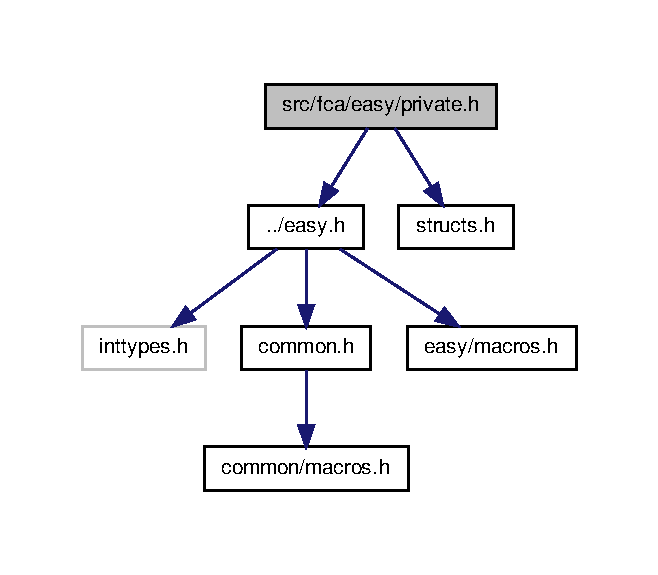
\includegraphics[width=350pt]{easy_2private_8h__incl}
\end{center}
\end{figure}
\-This graph shows which files directly or indirectly include this file\-:\nopagebreak
\begin{figure}[H]
\begin{center}
\leavevmode
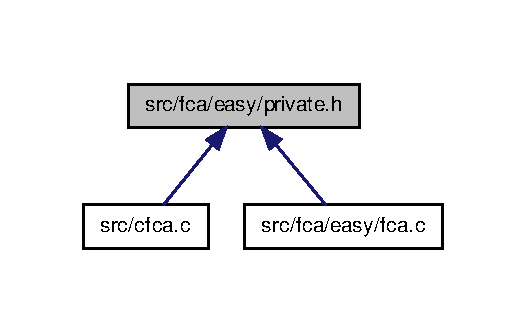
\includegraphics[width=350pt]{easy_2private_8h__dep__incl}
\end{center}
\end{figure}
\subsection*{\-Functions}
\begin{DoxyCompactItemize}
\item 
\hyperlink{easy_2structs_8h_ae552e1b13988c8c4ca0ab8f8a3e60f96}{my\-Formal\-Concept\-Intent\-Chunk} $\ast$ \hyperlink{easy_2private_8h_a10016c73379236582a412ab83e159618}{new\-Concept\-Chunk} (int attributes)
\begin{DoxyCompactList}\small\item\em \hyperlink{easy_2private_8h}{easy/private.\-h}, (c) 2013, \-Immanuel \-Albrecht; \-Dresden \-University of \-Technology, \-Professur für die \-Psychologie des \-Lernen und \-Lehrens \end{DoxyCompactList}\item 
void \hyperlink{easy_2private_8h_ad13aa7f16480d11c9c89310cca51670b}{delete\-Concept\-Chunk} (\hyperlink{easy_2structs_8h_ae552e1b13988c8c4ca0ab8f8a3e60f96}{my\-Formal\-Concept\-Intent\-Chunk} $\ast$$\ast$c)
\begin{DoxyCompactList}\small\item\em deletes a concept chunk object and sets its pointer to zero \end{DoxyCompactList}\item 
\hyperlink{easy_2structs_8h_a6c7fd90fd34d9ca52fedd96a01dd3566}{\-Formal\-Concept\-Intent\-Bulk\-List} \hyperlink{easy_2private_8h_a709ef22f213a99f6a46ca8aa78328ece}{new\-Concept\-Bulk} (int attributes)
\begin{DoxyCompactList}\small\item\em creates a new formal concept intent bulk list \end{DoxyCompactList}\item 
\hyperlink{easy_2structs_8h_a6c7fd90fd34d9ca52fedd96a01dd3566}{\-Formal\-Concept\-Intent\-Bulk\-List} \hyperlink{easy_2private_8h_a629cb24ff7d30d56d803e1848ff0019d}{new\-Concept\-Bulk\-From\-Context} (\hyperlink{easy_8h_ad53dc3fc96151a44387245e6481f95a4}{\-Formal\-Context} ctx)
\begin{DoxyCompactList}\small\item\em creates a new formal concept intent chunk and fills it with the intents of all formal concepts in the concept lattice of ctx, using next closure algorithm \end{DoxyCompactList}\item 
void \hyperlink{easy_2private_8h_ac1a973138b558d99763bfa84d022d42d}{write\-Concepts\-To\-File} (\hyperlink{easy_8h_ad53dc3fc96151a44387245e6481f95a4}{\-Formal\-Context} ctx, \hyperlink{easy_2structs_8h_a6c7fd90fd34d9ca52fedd96a01dd3566}{\-Formal\-Concept\-Intent\-Bulk\-List} root, const char $\ast$filename)
\begin{DoxyCompactList}\small\item\em write a list of concept intents into a .cxt file \end{DoxyCompactList}\item 
void \hyperlink{easy_2private_8h_acd989c02b03c2cc8bf2d477d2f5636e5}{delete\-Concept\-Bulk} (\hyperlink{easy_2structs_8h_a6c7fd90fd34d9ca52fedd96a01dd3566}{\-Formal\-Concept\-Intent\-Bulk\-List} $\ast$root\-Node)
\begin{DoxyCompactList}\small\item\em deletes the entire bulk list \end{DoxyCompactList}\item 
int \hyperlink{easy_2private_8h_a965bdc1065d581495114a764020c3c6b}{count\-Concepts\-In\-Bulk} (\hyperlink{easy_2structs_8h_a6c7fd90fd34d9ca52fedd96a01dd3566}{\-Formal\-Concept\-Intent\-Bulk\-List} root)
\begin{DoxyCompactList}\small\item\em use this for bulks that are filled in order \end{DoxyCompactList}\item 
\hyperlink{easy_2structs_8h_a6c7fd90fd34d9ca52fedd96a01dd3566}{\-Formal\-Concept\-Intent\-Bulk\-List} \hyperlink{easy_2private_8h_ac9e73d5390011291b92740d99f186ab4}{add\-Concept\-To\-Bulk} (\hyperlink{easy_2structs_8h_a6c7fd90fd34d9ca52fedd96a01dd3566}{\-Formal\-Concept\-Intent\-Bulk\-List} root, const \hyperlink{easy_8h_a92fa84ef7a12663bb998f141ab729056}{\-Incidence\-Cell} $\ast$intent)
\begin{DoxyCompactList}\small\item\em copies the given intent to the bulk denoted by the root node. \end{DoxyCompactList}\item 
void \hyperlink{easy_2private_8h_abdc733f4352afae86d46345b3288e052}{close\-Intent} (\hyperlink{easy_8h_ad53dc3fc96151a44387245e6481f95a4}{\-Formal\-Context} restrict ctx, const \hyperlink{easy_8h_a92fa84ef7a12663bb998f141ab729056}{\-Incidence\-Cell} $\ast$restrict input, \hyperlink{easy_8h_a92fa84ef7a12663bb998f141ab729056}{\-Incidence\-Cell} $\ast$restrict output)
\item 
void \hyperlink{easy_2private_8h_ac7782e7983ac6911f630994ee16eecbc}{close\-Intent2} (\hyperlink{easy_8h_ad53dc3fc96151a44387245e6481f95a4}{\-Formal\-Context} restrict ctx, const \hyperlink{easy_8h_a92fa84ef7a12663bb998f141ab729056}{\-Incidence\-Cell} $\ast$restrict input, \hyperlink{easy_8h_a92fa84ef7a12663bb998f141ab729056}{\-Incidence\-Cell} $\ast$restrict output\-Intent, \hyperlink{easy_8h_a92fa84ef7a12663bb998f141ab729056}{\-Incidence\-Cell} $\ast$restrict output\-Extent)
\begin{DoxyCompactList}\small\item\em close an attribute set, i.\-e. \end{DoxyCompactList}\item 
int \hyperlink{easy_2private_8h_a3eff21bebd55849e1049f6d8b6c50a8b}{intent\-Cmp} (int attributes, const \hyperlink{easy_8h_a92fa84ef7a12663bb998f141ab729056}{\-Incidence\-Cell} $\ast$minus, const \hyperlink{easy_8h_a92fa84ef7a12663bb998f141ab729056}{\-Incidence\-Cell} $\ast$plus)
\begin{DoxyCompactList}\small\item\em compare two intent vectors \end{DoxyCompactList}\end{DoxyCompactItemize}


\subsection{\-Function \-Documentation}
\hypertarget{easy_2private_8h_ac9e73d5390011291b92740d99f186ab4}{\index{easy/private.\-h@{easy/private.\-h}!add\-Concept\-To\-Bulk@{add\-Concept\-To\-Bulk}}
\index{add\-Concept\-To\-Bulk@{add\-Concept\-To\-Bulk}!easy/private.h@{easy/private.\-h}}
\subsubsection[{add\-Concept\-To\-Bulk}]{\setlength{\rightskip}{0pt plus 5cm}{\bf \-Formal\-Concept\-Intent\-Bulk\-List} {\bf add\-Concept\-To\-Bulk} (
\begin{DoxyParamCaption}
\item[{{\bf \-Formal\-Concept\-Intent\-Bulk\-List}}]{root, }
\item[{const {\bf \-Incidence\-Cell} $\ast$}]{intent}
\end{DoxyParamCaption}
)}}\label{easy_2private_8h_ac9e73d5390011291b92740d99f186ab4}


copies the given intent to the bulk denoted by the root node. 


\begin{DoxyParams}{\-Parameters}
{\em root} & root node of the bulk \\
\hline
{\em intent} & read-\/only pointer to an array of \-Incidence\-Cell\mbox{[}root-\/$>$attributes\mbox{]}\\
\hline
\end{DoxyParams}
\begin{DoxyReturn}{\-Returns}
the node where the intent was added to the last chunk 
\end{DoxyReturn}


\-Definition at line 423 of file fca.\-c.



\-References s\-Formal\-Concept\-Intent\-Bulk\-Node\-::attributes, \-B\-U\-L\-K\-S\-I\-Z\-E, \-C\-E\-L\-L, s\-Formal\-Concept\-Intent\-Bulk\-Node\-::chunks, \-C\-H\-U\-N\-K\-S\-I\-Z\-E, new\-Concept\-Bulk, new\-Concept\-Chunk, s\-Formal\-Concept\-Intent\-Bulk\-Node\-::next, \-R\-E\-T\-U\-R\-N\-\_\-\-Z\-E\-R\-O\-\_\-\-I\-F\-\_\-\-Z\-E\-R\-O, smy\-Formal\-Concept\-Intent\-Chunk\-::size, and s\-Formal\-Concept\-Intent\-Bulk\-Node\-::size.


\begin{DoxyCode}
{
    RETURN_ZERO_IF_ZERO(root);

    do
    {

        if (root->size == 0)
        {
            root->chunks[0] = newConceptChunk(root->attributes);
            root->size = 1;
        }

        int last_index;
        last_index = root->size - 1;

        if (root->chunks[last_index]->size == CHUNKSIZE)
        {
            if (root->size == BULKSIZE)
            {
                if (root->next == 0)
                {
                    root->next = newConceptBulk(root->attributes);
                }
                root = root->next;
                continue;
            }
            else
            {
                last_index = root->size++;
                root->chunks[last_index] = newConceptChunk(root->attributes);
            }
        }

#pragma GCC diagnostic push
#pragma GCC diagnostic ignored "-Wsign-conversion"

        memcpy(
                &(CELL(root->chunks[last_index]->size, root->chunks[last_index]
      ,0)),
                intent, sizeof(IncidenceCell) * root->attributes);

#pragma GCC diagnostic pop

        root->chunks[last_index]->size++;

        break;

    } while (1);

    return root;
}
\end{DoxyCode}
\hypertarget{easy_2private_8h_abdc733f4352afae86d46345b3288e052}{\index{easy/private.\-h@{easy/private.\-h}!close\-Intent@{close\-Intent}}
\index{close\-Intent@{close\-Intent}!easy/private.h@{easy/private.\-h}}
\subsubsection[{close\-Intent}]{\setlength{\rightskip}{0pt plus 5cm}void {\bf close\-Intent} (
\begin{DoxyParamCaption}
\item[{{\bf \-Formal\-Context} restrict}]{ctx, }
\item[{const {\bf \-Incidence\-Cell} $\ast$restrict}]{input, }
\item[{{\bf \-Incidence\-Cell} $\ast$restrict}]{output}
\end{DoxyParamCaption}
)}}\label{easy_2private_8h_abdc733f4352afae86d46345b3288e052}
\hypertarget{easy_2private_8h_ac7782e7983ac6911f630994ee16eecbc}{\index{easy/private.\-h@{easy/private.\-h}!close\-Intent2@{close\-Intent2}}
\index{close\-Intent2@{close\-Intent2}!easy/private.h@{easy/private.\-h}}
\subsubsection[{close\-Intent2}]{\setlength{\rightskip}{0pt plus 5cm}void {\bf close\-Intent2} (
\begin{DoxyParamCaption}
\item[{{\bf \-Formal\-Context} restrict}]{ctx, }
\item[{const {\bf \-Incidence\-Cell} $\ast$restrict}]{input, }
\item[{{\bf \-Incidence\-Cell} $\ast$restrict}]{output\-Intent, }
\item[{{\bf \-Incidence\-Cell} $\ast$restrict}]{output\-Extent}
\end{DoxyParamCaption}
)}}\label{easy_2private_8h_ac7782e7983ac6911f630994ee16eecbc}


close an attribute set, i.\-e. 

add further attributes, 1.\-92 times slower than close\-Intent


\begin{DoxyParams}{\-Parameters}
{\em ctx} & formal context \\
\hline
{\em input} & the intent set that is to be closed \\
\hline
{\em output\-Intent} & the closure intent'' wrt. ctx \\
\hline
{\em output\-Extent} & the corresponding objects, i.\-e. intent' wrt. ctx \\
\hline
\end{DoxyParams}


\-Definition at line 487 of file fca.\-c.



\-References \-C\-L\-E\-A\-R, \-C\-R\-O\-S\-S, g\-Im, and \-I\-N\-C\-I\-D\-E\-S.


\begin{DoxyCode}
{
    myFormalContext* restrict I;
    I = (myFormalContext*) ctx;

    for (int g = 0; g < I->objects; ++g)
    {
        CROSS(outputExtent[g]);
        for (int m = 0; m < I->attributes; ++m)
        {
            if (INCIDES(input[m]))
                if (!gIm(g,I,m))
                {
                    /*
                     * some attribute is not present for this object -> next
       object
                     */
                    CLEAR(outputExtent[g]);
                    break;
                }
        }
    }

    for (int m = 0; m < I->attributes; ++m)
    {
        CROSS(outputIntent[m]);
        for (int g = 0; g < I->objects; ++g)
        {
            if (INCIDES(outputExtent[g]))
                if (!gIm(g,I,m))
                {
                    CLEAR(outputIntent[m]);
                    break;
                }
        }
    }

}
\end{DoxyCode}
\hypertarget{easy_2private_8h_a965bdc1065d581495114a764020c3c6b}{\index{easy/private.\-h@{easy/private.\-h}!count\-Concepts\-In\-Bulk@{count\-Concepts\-In\-Bulk}}
\index{count\-Concepts\-In\-Bulk@{count\-Concepts\-In\-Bulk}!easy/private.h@{easy/private.\-h}}
\subsubsection[{count\-Concepts\-In\-Bulk}]{\setlength{\rightskip}{0pt plus 5cm}int {\bf count\-Concepts\-In\-Bulk} (
\begin{DoxyParamCaption}
\item[{{\bf \-Formal\-Concept\-Intent\-Bulk\-List}}]{root}
\end{DoxyParamCaption}
)}}\label{easy_2private_8h_a965bdc1065d581495114a764020c3c6b}


use this for bulks that are filled in order 


\begin{DoxyParams}{\-Parameters}
{\em root} & \\
\hline
\end{DoxyParams}
\begin{DoxyReturn}{\-Returns}
number of concepts in bulk 
\end{DoxyReturn}


\-Definition at line 388 of file fca.\-c.



\-References s\-Formal\-Concept\-Intent\-Bulk\-Node\-::chunks, \-C\-H\-U\-N\-K\-S\-I\-Z\-E, s\-Formal\-Concept\-Intent\-Bulk\-Node\-::next, \-R\-E\-T\-U\-R\-N\-\_\-\-Z\-E\-R\-O\-\_\-\-I\-F\-\_\-\-Z\-E\-R\-O, smy\-Formal\-Concept\-Intent\-Chunk\-::size, and s\-Formal\-Concept\-Intent\-Bulk\-Node\-::size.


\begin{DoxyCode}
{
    RETURN_ZERO_IF_ZERO(root);

    int count = 0;

    while (root != 0)
    {
        if (root->size > 0)
        {
            /*
             * count the full chunks
             */
            count += CHUNKSIZE * (root->size - 1);
            /*
             * and the last chunk
             */
            count += root->chunks[root->size - 1]->size;
        }
        root = root->next;
    }

    return count;
}
\end{DoxyCode}
\hypertarget{easy_2private_8h_acd989c02b03c2cc8bf2d477d2f5636e5}{\index{easy/private.\-h@{easy/private.\-h}!delete\-Concept\-Bulk@{delete\-Concept\-Bulk}}
\index{delete\-Concept\-Bulk@{delete\-Concept\-Bulk}!easy/private.h@{easy/private.\-h}}
\subsubsection[{delete\-Concept\-Bulk}]{\setlength{\rightskip}{0pt plus 5cm}void {\bf delete\-Concept\-Bulk} (
\begin{DoxyParamCaption}
\item[{{\bf \-Formal\-Concept\-Intent\-Bulk\-List} $\ast$}]{root\-Node}
\end{DoxyParamCaption}
)}}\label{easy_2private_8h_acd989c02b03c2cc8bf2d477d2f5636e5}


deletes the entire bulk list 


\begin{DoxyParams}{\-Parameters}
{\em root\-Node} & pointer to the first node \\
\hline
\end{DoxyParams}


\-Definition at line 356 of file fca.\-c.



\-References s\-Formal\-Concept\-Intent\-Bulk\-Node\-::chunks, delete\-Concept\-Chunk, s\-Formal\-Concept\-Intent\-Bulk\-Node\-::next, \-R\-E\-T\-U\-R\-N\-\_\-\-I\-F\-\_\-\-Z\-E\-R\-O, and s\-Formal\-Concept\-Intent\-Bulk\-Node\-::size.


\begin{DoxyCode}
{
    RETURN_IF_ZERO(rootNode);
    RETURN_IF_ZERO(*rootNode);

    FormalConceptIntentBulkList l;
    l = *rootNode;
    *rootNode = 0;

    do
    {
        for (int var = 0; var < l->size; ++var)
        {
            deleteConceptChunk(&(l->chunks[var]));
        }

        FormalConceptIntentBulkList next;
        next = l->next;

        free(l->chunks);
        free(l);

        l = next;
    } while (l != 0);
}
\end{DoxyCode}
\hypertarget{easy_2private_8h_ad13aa7f16480d11c9c89310cca51670b}{\index{easy/private.\-h@{easy/private.\-h}!delete\-Concept\-Chunk@{delete\-Concept\-Chunk}}
\index{delete\-Concept\-Chunk@{delete\-Concept\-Chunk}!easy/private.h@{easy/private.\-h}}
\subsubsection[{delete\-Concept\-Chunk}]{\setlength{\rightskip}{0pt plus 5cm}void {\bf delete\-Concept\-Chunk} (
\begin{DoxyParamCaption}
\item[{{\bf my\-Formal\-Concept\-Intent\-Chunk} $\ast$$\ast$}]{c}
\end{DoxyParamCaption}
)}}\label{easy_2private_8h_ad13aa7f16480d11c9c89310cca51670b}


deletes a concept chunk object and sets its pointer to zero 


\begin{DoxyParams}{\-Parameters}
{\em c} & pointer to the concept chunk to be deleted \\
\hline
\end{DoxyParams}


\-Definition at line 321 of file fca.\-c.



\-References \-R\-E\-T\-U\-R\-N\-\_\-\-I\-F\-\_\-\-Z\-E\-R\-O.


\begin{DoxyCode}
{
    RETURN_IF_ZERO(c);
    RETURN_IF_ZERO(*c);

    free((*c)->incidence);

    free(*c);
    *c = 0;
}
\end{DoxyCode}
\hypertarget{easy_2private_8h_a3eff21bebd55849e1049f6d8b6c50a8b}{\index{easy/private.\-h@{easy/private.\-h}!intent\-Cmp@{intent\-Cmp}}
\index{intent\-Cmp@{intent\-Cmp}!easy/private.h@{easy/private.\-h}}
\subsubsection[{intent\-Cmp}]{\setlength{\rightskip}{0pt plus 5cm}int {\bf intent\-Cmp} (
\begin{DoxyParamCaption}
\item[{int}]{attributes, }
\item[{const {\bf \-Incidence\-Cell} $\ast$}]{minus, }
\item[{const {\bf \-Incidence\-Cell} $\ast$}]{plus}
\end{DoxyParamCaption}
)}}\label{easy_2private_8h_a3eff21bebd55849e1049f6d8b6c50a8b}


compare two intent vectors 


\begin{DoxyParams}{\-Parameters}
{\em attributes} & attribute count \\
\hline
{\em minus} & \char`\"{}left\char`\"{} operand \\
\hline
{\em plus} & \char`\"{}right\char`\"{} operand \\
\hline
\end{DoxyParams}
\begin{DoxyReturn}{\-Returns}
-\/1 if minus is bigger, 1 if plus is bigger, 0 if minus and plus is the same 
\end{DoxyReturn}


\-Definition at line 587 of file fca.\-c.



\-References \-I\-N\-C\-I\-D\-E\-S.


\begin{DoxyCode}
{
    for (int var = 0; var < attributes; ++var)
    {
        if (INCIDES(minus[var]))
        {
            if (!INCIDES((plus[var])))
                return -1;
        }
        else if (INCIDES(plus[var]))
        {
            return 1;
        }
    }
    return 0;
}
\end{DoxyCode}
\hypertarget{easy_2private_8h_a709ef22f213a99f6a46ca8aa78328ece}{\index{easy/private.\-h@{easy/private.\-h}!new\-Concept\-Bulk@{new\-Concept\-Bulk}}
\index{new\-Concept\-Bulk@{new\-Concept\-Bulk}!easy/private.h@{easy/private.\-h}}
\subsubsection[{new\-Concept\-Bulk}]{\setlength{\rightskip}{0pt plus 5cm}{\bf \-Formal\-Concept\-Intent\-Bulk\-List} {\bf new\-Concept\-Bulk} (
\begin{DoxyParamCaption}
\item[{int}]{attributes}
\end{DoxyParamCaption}
)}}\label{easy_2private_8h_a709ef22f213a99f6a46ca8aa78328ece}


creates a new formal concept intent bulk list 


\begin{DoxyParams}{\-Parameters}
{\em attributes} & number of attributes of the concept intents \\
\hline
\end{DoxyParams}
\begin{DoxyReturn}{\-Returns}
new formal concept intent bulk list's first node 
\end{DoxyReturn}


\-Definition at line 339 of file fca.\-c.



\-References s\-Formal\-Concept\-Intent\-Bulk\-Node\-::attributes, \-B\-U\-L\-K\-S\-I\-Z\-E, s\-Formal\-Concept\-Intent\-Bulk\-Node\-::chunks, s\-Formal\-Concept\-Intent\-Bulk\-Node\-::next, and s\-Formal\-Concept\-Intent\-Bulk\-Node\-::size.


\begin{DoxyCode}
{
    FormalConceptIntentBulkList l;
    l = malloc(sizeof(struct sFormalConceptIntentBulkNode));

    l->attributes = attributes;
    l->size = 0;
    l->chunks = calloc(BULKSIZE, sizeof(myFormalConceptIntentChunk*));
    l->next = 0;
    return l;
}
\end{DoxyCode}
\hypertarget{easy_2private_8h_a629cb24ff7d30d56d803e1848ff0019d}{\index{easy/private.\-h@{easy/private.\-h}!new\-Concept\-Bulk\-From\-Context@{new\-Concept\-Bulk\-From\-Context}}
\index{new\-Concept\-Bulk\-From\-Context@{new\-Concept\-Bulk\-From\-Context}!easy/private.h@{easy/private.\-h}}
\subsubsection[{new\-Concept\-Bulk\-From\-Context}]{\setlength{\rightskip}{0pt plus 5cm}{\bf \-Formal\-Concept\-Intent\-Bulk\-List} {\bf new\-Concept\-Bulk\-From\-Context} (
\begin{DoxyParamCaption}
\item[{{\bf \-Formal\-Context}}]{ctx}
\end{DoxyParamCaption}
)}}\label{easy_2private_8h_a629cb24ff7d30d56d803e1848ff0019d}


creates a new formal concept intent chunk and fills it with the intents of all formal concepts in the concept lattice of ctx, using next closure algorithm 


\begin{DoxyParams}{\-Parameters}
{\em ctx} & formal context \\
\hline
\end{DoxyParams}
\begin{DoxyReturn}{\-Returns}
concept intents 
\end{DoxyReturn}


\-Definition at line 612 of file fca.\-c.



\-References add\-Concept\-To\-Bulk, smy\-Formal\-Context\-::attributes, \-C\-L\-E\-A\-R, close\-Intent, \-C\-R\-O\-S\-S, \-I\-N\-C\-I\-D\-E\-S, new\-Concept\-Bulk, and \-R\-E\-T\-U\-R\-N\-\_\-\-Z\-E\-R\-O\-\_\-\-I\-F\-\_\-\-Z\-E\-R\-O.


\begin{DoxyCode}
{
    RETURN_ZERO_IF_ZERO(ctx);

    myFormalContext *c;
    c = (myFormalContext*) ctx;

    IncidenceCell *M;
    IncidenceCell *Y;

#pragma GCC diagnostic push
#pragma GCC diagnostic ignored "-Wsign-conversion"

    Y = calloc(c->attributes, sizeof(IncidenceCell));
    M = malloc(c->attributes * sizeof(IncidenceCell));

#pragma GCC diagnostic pop

    /*
     * calculate the bottom intent of the concept lattice, i.e. {}''
     */
    closeIntent(ctx, Y, M);

    FormalConceptIntentBulkList root;
    FormalConceptIntentBulkList last;

    root = newConceptBulk(c->attributes);

    /*
     * add the bottom element of the concept lattice (a concept lattice is
       never empty)
     */

    last = addConceptToBulk(root, M);

    /*
     * begin of nextClosure function iteration
     */
    nextClosure:

    for (int i = c->attributes - 1; i >= 0; --i)
    {

        if (!INCIDES(M[i]))
        {
            CROSS(M[i]);
            closeIntent(ctx, M, Y);

            int good;
            good = 1;

            for (int j = 0; j < i; ++j)
            {
                if (INCIDES(Y[j]))
                {
                    if (!INCIDES((M[j])))
                    {

                        good = 0;
                        break;
                    }
                }
            }
            if (good)
            {
                /*
                 * we found the next intent
                 */
                last = addConceptToBulk(last, Y);

                /*
                 * continue with Y for M
                 */

                IncidenceCell *DELTA;
                DELTA = M;
                M = Y;
                Y = DELTA;
                /*
                 * do the nextClosure
                 */
                goto nextClosure;
            }
        }

        CLEAR(M[i]);
    }

    /*
     * free up memory
     */

    free(M);
    free(Y);
    return root;
}
\end{DoxyCode}
\hypertarget{easy_2private_8h_a10016c73379236582a412ab83e159618}{\index{easy/private.\-h@{easy/private.\-h}!new\-Concept\-Chunk@{new\-Concept\-Chunk}}
\index{new\-Concept\-Chunk@{new\-Concept\-Chunk}!easy/private.h@{easy/private.\-h}}
\subsubsection[{new\-Concept\-Chunk}]{\setlength{\rightskip}{0pt plus 5cm}{\bf my\-Formal\-Concept\-Intent\-Chunk}$\ast$ {\bf new\-Concept\-Chunk} (
\begin{DoxyParamCaption}
\item[{int}]{attributes}
\end{DoxyParamCaption}
)}}\label{easy_2private_8h_a10016c73379236582a412ab83e159618}


\hyperlink{easy_2private_8h}{easy/private.\-h}, (c) 2013, \-Immanuel \-Albrecht; \-Dresden \-University of \-Technology, \-Professur für die \-Psychologie des \-Lernen und \-Lehrens 

\-This program is free software\-: you can redistribute it and/or modify it under the terms of the \-G\-N\-U \-General \-Public \-License as published by the \-Free \-Software \-Foundation, either version 3 of the \-License, or (at your option) any later version.

\-This program is distributed in the hope that it will be useful, but \-W\-I\-T\-H\-O\-U\-T \-A\-N\-Y \-W\-A\-R\-R\-A\-N\-T\-Y; without even the implied warranty of \-M\-E\-R\-C\-H\-A\-N\-T\-A\-B\-I\-L\-I\-T\-Y or \-F\-I\-T\-N\-E\-S\-S \-F\-O\-R \-A \-P\-A\-R\-T\-I\-C\-U\-L\-A\-R \-P\-U\-R\-P\-O\-S\-E. \-See the \-G\-N\-U \-General \-Public \-License for more details.

\-You should have received a copy of the \-G\-N\-U \-General \-Public \-License along with this program. \-If not, see $<$\href{http://www.gnu.org/licenses/}{\tt http\-://www.\-gnu.\-org/licenses/}$>$.

\hyperlink{easy_2private_8h}{easy/private.\-h}, (c) 2013, \-Immanuel \-Albrecht; \-Dresden \-University of \-Technology, \-Professur für die \-Psychologie des \-Lernen und \-Lehrens


\begin{DoxyParams}{\-Parameters}
{\em attributes} & number of attributes of the hosting formal context \\
\hline
\end{DoxyParams}
\begin{DoxyReturn}{\-Returns}
a new concept chunk object 
\end{DoxyReturn}


\-Definition at line 298 of file fca.\-c.



\-References smy\-Formal\-Concept\-Intent\-Chunk\-::attributes, \-C\-H\-U\-N\-K\-S\-I\-Z\-E, smy\-Formal\-Concept\-Intent\-Chunk\-::incidence, and smy\-Formal\-Concept\-Intent\-Chunk\-::size.


\begin{DoxyCode}
{
    myFormalConceptIntentChunk *c;
    c = malloc(sizeof(myFormalConceptIntentChunk));
    c->attributes = attributes;
    c->size = 0;

#pragma GCC diagnostic push
#pragma GCC diagnostic ignored "-Wsign-conversion"

    c->incidence = calloc(attributes * CHUNKSIZE, sizeof(IncidenceCell));

#pragma GCC diagnostic pop

    return c;
}
\end{DoxyCode}
\hypertarget{easy_2private_8h_ac1a973138b558d99763bfa84d022d42d}{\index{easy/private.\-h@{easy/private.\-h}!write\-Concepts\-To\-File@{write\-Concepts\-To\-File}}
\index{write\-Concepts\-To\-File@{write\-Concepts\-To\-File}!easy/private.h@{easy/private.\-h}}
\subsubsection[{write\-Concepts\-To\-File}]{\setlength{\rightskip}{0pt plus 5cm}void {\bf write\-Concepts\-To\-File} (
\begin{DoxyParamCaption}
\item[{{\bf \-Formal\-Context}}]{ctx, }
\item[{{\bf \-Formal\-Concept\-Intent\-Bulk\-List}}]{root, }
\item[{const char $\ast$}]{filename}
\end{DoxyParamCaption}
)}}\label{easy_2private_8h_ac1a973138b558d99763bfa84d022d42d}


write a list of concept intents into a .cxt file 


\begin{DoxyParams}{\-Parameters}
{\em ctx} & formal context (or 0, is used for attribute names) \\
\hline
{\em root} & the first node of the formal concept intent bulk \\
\hline
{\em filename} & output file name (.cxt) \\
\hline
\end{DoxyParams}


\-Definition at line 716 of file fca.\-c.



\-References smy\-Formal\-Context\-::attribute\-Names, smy\-Formal\-Context\-::attributes, s\-Formal\-Concept\-Intent\-Bulk\-Node\-::attributes, s\-Formal\-Concept\-Intent\-Bulk\-Node\-::chunks, count\-Concepts\-In\-Bulk, g\-Im, s\-Formal\-Concept\-Intent\-Bulk\-Node\-::next, \-R\-E\-T\-U\-R\-N\-\_\-\-I\-F\-\_\-\-Z\-E\-R\-O, smy\-Formal\-Concept\-Intent\-Chunk\-::size, s\-Formal\-Concept\-Intent\-Bulk\-Node\-::size, and \-W\-A\-R\-N\-\_\-\-I\-F\-\_\-\-U\-N\-E\-Q\-U\-A\-L\-\_\-\-D\-O.


\begin{DoxyCode}
{
    RETURN_IF_ZERO(root);

    myFormalContext* c;

    if (ctx != 0)
    {
        c = (myFormalContext*) ctx;

        WARN_IF_UNEQUAL_DO(c->attributes, root->attributes, c = 0);
    }
    else
    {
        c = 0;
    }

    RETURN_IF_ZERO(filename);

    FILE* file;
    file = fopen(filename, "w");

    RETURN_IF_ZERO(file);

    int objects;
    objects = countConceptsInBulk(root);

    fprintf(file, "B\n\n%d\n%d\n\n", objects, root->attributes);

    for (int var = 0; var < objects; ++var)
    {
        fprintf(file, "C%8d\n", (var + 1));
    }

    if (c != 0)
    {
        for (int var = 0; var < c->attributes; ++var)
        {
            fputs(c->attributeNames[var], file);
            fputs("\n", file);
        }
    }
    else
    {
        for (int var = 0; var < root->attributes; ++var)
        {
            fprintf(file, "m%8d\n", (var + 1));
        }
    }

    for (; root != 0; root = root->next)
    {
        for (int chunk = 0; chunk < root->size; ++chunk)
        {
            for (int g = 0; g < root->chunks[chunk]->size; ++g)
            {
                for (int m = 0; m < root->attributes; ++m)
                {
                    if ( gIm(g, root->chunks[chunk], m))
                        fputs("X", file);
                    else
                        fputs(".", file);
                }
                fputs("\n", file);
            }
        }
    }

    fclose(file);

}
\end{DoxyCode}

\hypertarget{vector_2private_8h}{\section{src/fca/vector/private.h \-File \-Reference}
\label{vector_2private_8h}\index{src/fca/vector/private.\-h@{src/fca/vector/private.\-h}}
}
{\ttfamily \#include \char`\"{}../vector.\-h\char`\"{}}\*
{\ttfamily \#include \char`\"{}structs.\-h\char`\"{}}\*
\-Include dependency graph for private.\-h\-:
\nopagebreak
\begin{figure}[H]
\begin{center}
\leavevmode
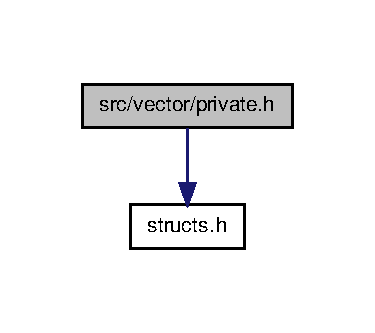
\includegraphics[width=350pt]{vector_2private_8h__incl}
\end{center}
\end{figure}
\-This graph shows which files directly or indirectly include this file\-:\nopagebreak
\begin{figure}[H]
\begin{center}
\leavevmode
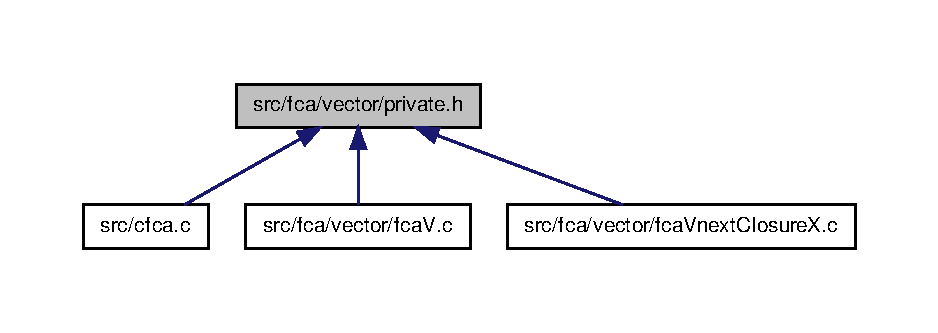
\includegraphics[width=350pt]{vector_2private_8h__dep__incl}
\end{center}
\end{figure}
\subsection*{\-Functions}
\begin{DoxyCompactItemize}
\item 
void \hyperlink{vector_2private_8h_aa30fbd99dd8ad4cee19d32d5debf9e07}{close\-Intent\-V} (\hyperlink{vector_8h_a98aafc7ce3efff805e9add08680b731f}{\-Formal\-Context\-V} restrict ctx, const \hyperlink{vector_8h_aae617489ac88fff15979050721fe581f}{\-Incidence\-Vector} restrict input, \hyperlink{vector_8h_aae617489ac88fff15979050721fe581f}{\-Incidence\-Vector} restrict output)
\begin{DoxyCompactList}\small\item\em \hyperlink{vector_2private_8h}{vector/private.\-h}, (c) 2013, \-Immanuel \-Albrecht; \-Dresden \-University of \-Technology, \-Professur für die \-Psychologie des \-Lernen und \-Lehrens \end{DoxyCompactList}\item 
int \hyperlink{vector_2private_8h_a55d40e1b5169e4466d00cb930c67e0ef}{intent\-Cmp\-V} (size\-\_\-t attributes, const \hyperlink{vector_8h_aae617489ac88fff15979050721fe581f}{\-Incidence\-Vector} minus, const \hyperlink{vector_8h_aae617489ac88fff15979050721fe581f}{\-Incidence\-Vector} plus)
\begin{DoxyCompactList}\small\item\em compare two intent vectors \end{DoxyCompactList}\item 
\hyperlink{vector_2structs_8h_abe3c190ec3375121cbfe3afff517b9b9}{my\-Formal\-Concept\-Intent\-Chunk\-V} $\ast$ \hyperlink{vector_2private_8h_ab5c9a71c810ad1eeeb5f8ff78d77d899}{new\-Concept\-Chunk\-V} (size\-\_\-t attributes)
\begin{DoxyCompactList}\small\item\em create a new formal concept chunk \end{DoxyCompactList}\item 
void \hyperlink{vector_2private_8h_afd9305761d657be7c21fb81e82d72a42}{delete\-Concept\-Chunk\-V} (\hyperlink{vector_2structs_8h_abe3c190ec3375121cbfe3afff517b9b9}{my\-Formal\-Concept\-Intent\-Chunk\-V} $\ast$$\ast$c)
\begin{DoxyCompactList}\small\item\em deletes a concept chunk object and sets its pointer to zero \end{DoxyCompactList}\item 
\hyperlink{vector_2structs_8h_a6306c91d1e7b5237618bab6172a784a1}{\-Formal\-Concept\-Intent\-Bulk\-List\-V} \hyperlink{vector_2private_8h_abda612c4305c29a37b6501e18d94ebc5}{new\-Concept\-Bulk\-V} (size\-\_\-t attributes)
\begin{DoxyCompactList}\small\item\em creates a new formal concept intent bulk list \end{DoxyCompactList}\item 
\hyperlink{vector_2structs_8h_a6306c91d1e7b5237618bab6172a784a1}{\-Formal\-Concept\-Intent\-Bulk\-List\-V} \hyperlink{vector_2private_8h_a90151fdf1b3ef3201deb2e1ab752729d}{new\-Concept\-Bulk\-From\-Context\-V} (\hyperlink{vector_8h_a98aafc7ce3efff805e9add08680b731f}{\-Formal\-Context\-V} ctx)
\begin{DoxyCompactList}\small\item\em creates a new formal concept intent chunk and fills it with the intents of all formal concepts in the concept lattice of ctx, using next closure algorithm \end{DoxyCompactList}\item 
void \hyperlink{vector_2private_8h_ac1443261c57cc1d3db9361c188cd9c96}{write\-Concepts\-To\-File\-V} (\hyperlink{vector_8h_a98aafc7ce3efff805e9add08680b731f}{\-Formal\-Context\-V} ctx, \hyperlink{vector_2structs_8h_a6306c91d1e7b5237618bab6172a784a1}{\-Formal\-Concept\-Intent\-Bulk\-List\-V} root, const char $\ast$filename)
\begin{DoxyCompactList}\small\item\em write a list of concept intents into a .cxt file \end{DoxyCompactList}\item 
void \hyperlink{vector_2private_8h_aa2cf22779998982c65e3762c7e2c2c84}{delete\-Concept\-Bulk\-V} (\hyperlink{vector_2structs_8h_a6306c91d1e7b5237618bab6172a784a1}{\-Formal\-Concept\-Intent\-Bulk\-List\-V} $\ast$root\-Node)
\begin{DoxyCompactList}\small\item\em deletes the entire bulk list \end{DoxyCompactList}\item 
size\-\_\-t \hyperlink{vector_2private_8h_a7d53642e5953e35c86ef0425858d707e}{count\-Concepts\-In\-Bulk\-V} (\hyperlink{vector_2structs_8h_a6306c91d1e7b5237618bab6172a784a1}{\-Formal\-Concept\-Intent\-Bulk\-List\-V} root)
\begin{DoxyCompactList}\small\item\em use this for bulks that are filled in order \end{DoxyCompactList}\item 
\hyperlink{vector_2structs_8h_a6306c91d1e7b5237618bab6172a784a1}{\-Formal\-Concept\-Intent\-Bulk\-List\-V} \hyperlink{vector_2private_8h_aa6cc62f8dfd08ef795a932cd06e69b91}{add\-Concept\-To\-Bulk\-V} (\hyperlink{vector_2structs_8h_a6306c91d1e7b5237618bab6172a784a1}{\-Formal\-Concept\-Intent\-Bulk\-List\-V} root, const \hyperlink{vector_8h_aae617489ac88fff15979050721fe581f}{\-Incidence\-Vector} intent)
\begin{DoxyCompactList}\small\item\em copies the given intent to the bulk denoted by the root node. \end{DoxyCompactList}\item 
\hyperlink{vector_2structs_8h_a6306c91d1e7b5237618bab6172a784a1}{\-Formal\-Concept\-Intent\-Bulk\-List\-V} \hyperlink{vector_2private_8h_a8ee9a9ab122e4e5e8c5148ef759172f2}{next\-Closure\-V\-X1} (\hyperlink{vector_8h_a98aafc7ce3efff805e9add08680b731f}{\-Formal\-Context\-V} ctx, const \hyperlink{vector_8h_aae617489ac88fff15979050721fe581f}{\-Incidence\-Vector} restrict start, const \hyperlink{vector_8h_aae617489ac88fff15979050721fe581f}{\-Incidence\-Vector} restrict stop)
\begin{DoxyCompactList}\small\item\em creates a new formal concept intent chunk and fills it with the intents of all formal concepts in the concept lattice of ctx, using next closure algorithm, that are in a given lexicographic interval of the powerset \end{DoxyCompactList}\item 
\hyperlink{vector_2structs_8h_a6306c91d1e7b5237618bab6172a784a1}{\-Formal\-Concept\-Intent\-Bulk\-List\-V} \hyperlink{vector_2private_8h_a858241e44987c35c2ae688f2797f2a30}{next\-Closure\-V\-X} (\hyperlink{vector_8h_a98aafc7ce3efff805e9add08680b731f}{\-Formal\-Context\-V} ctx)
\begin{DoxyCompactList}\small\item\em creates a new formal concept intent chunk and fills it with the intents of all formal concepts in the concept lattice of ctx, using a parallel next closure algorithm with up to 8 threads \end{DoxyCompactList}\end{DoxyCompactItemize}


\subsection{\-Function \-Documentation}
\hypertarget{vector_2private_8h_aa6cc62f8dfd08ef795a932cd06e69b91}{\index{vector/private.\-h@{vector/private.\-h}!add\-Concept\-To\-Bulk\-V@{add\-Concept\-To\-Bulk\-V}}
\index{add\-Concept\-To\-Bulk\-V@{add\-Concept\-To\-Bulk\-V}!vector/private.h@{vector/private.\-h}}
\subsubsection[{add\-Concept\-To\-Bulk\-V}]{\setlength{\rightskip}{0pt plus 5cm}{\bf \-Formal\-Concept\-Intent\-Bulk\-List\-V} {\bf add\-Concept\-To\-Bulk\-V} (
\begin{DoxyParamCaption}
\item[{{\bf \-Formal\-Concept\-Intent\-Bulk\-List\-V}}]{root, }
\item[{const {\bf \-Incidence\-Vector}}]{intent}
\end{DoxyParamCaption}
)}}\label{vector_2private_8h_aa6cc62f8dfd08ef795a932cd06e69b91}


copies the given intent to the bulk denoted by the root node. 


\begin{DoxyParams}{\-Parameters}
{\em root} & root node of the bulk \\
\hline
{\em intent} & read-\/only pointer to an array of \-Incidence\-Cell\mbox{[}root-\/$>$attributes\mbox{]}\\
\hline
\end{DoxyParams}
\begin{DoxyReturn}{\-Returns}
the node where the intent was added to the last chunk 
\end{DoxyReturn}


\-Definition at line 828 of file fca\-V.\-c.



\-References s\-Formal\-Concept\-Intent\-Bulk\-Node\-V\-::attributes, \-B\-U\-L\-K\-S\-I\-Z\-E\-V, s\-Formal\-Concept\-Intent\-Bulk\-Node\-V\-::chunks, \-C\-H\-U\-N\-K\-S\-I\-Z\-E\-V, new\-Concept\-Bulk\-V(), new\-Concept\-Chunk\-V(), s\-Formal\-Concept\-Intent\-Bulk\-Node\-V\-::next, \-R\-E\-T\-U\-R\-N\-\_\-\-Z\-E\-R\-O\-\_\-\-I\-F\-\_\-\-Z\-E\-R\-O, \-R\-O\-W, smy\-Formal\-Concept\-Intent\-Chunk\-V\-::size, s\-Formal\-Concept\-Intent\-Bulk\-Node\-V\-::size, and s\-Formal\-Concept\-Intent\-Bulk\-Node\-V\-::width.



\-Referenced by new\-Concept\-Bulk\-From\-Context\-V(), and next\-Closure\-V\-X1().


\begin{DoxyCode}
{
    RETURN_ZERO_IF_ZERO(root);

    do
    {

        if (root->size == 0)
        {
            root->chunks[0] = newConceptChunkV(root->attributes);
            root->size = 1;
        }

        size_t last_index;
        last_index = root->size - 1;

        if (root->chunks[last_index]->size == CHUNKSIZEV)
        {
            if (root->size == BULKSIZEV)
            {
                if (root->next == 0)
                {
                    root->next = newConceptBulkV(root->attributes);
                }
                root = root->next;
                continue;
            }
            else
            {
                last_index = root->size++;
                root->chunks[last_index] = newConceptChunkV(root->attributes);
            }
        }

#pragma GCC diagnostic push
#pragma GCC diagnostic ignored "-Wsign-conversion"

        memcpy( ROW(root->chunks[last_index]->size, root->chunks[last_index]),
                intent, sizeof(uint64_t) * root->width);

#pragma GCC diagnostic pop

        root->chunks[last_index]->size++;

        break;

    } while (1);

    return root;
}
\end{DoxyCode}


\-Here is the call graph for this function\-:\nopagebreak
\begin{figure}[H]
\begin{center}
\leavevmode
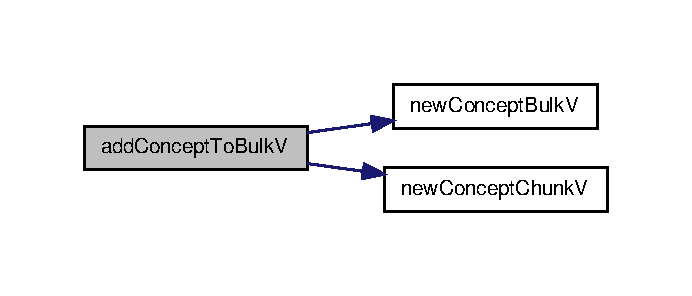
\includegraphics[width=332pt]{vector_2private_8h_aa6cc62f8dfd08ef795a932cd06e69b91_cgraph}
\end{center}
\end{figure}


\hypertarget{vector_2private_8h_aa30fbd99dd8ad4cee19d32d5debf9e07}{\index{vector/private.\-h@{vector/private.\-h}!close\-Intent\-V@{close\-Intent\-V}}
\index{close\-Intent\-V@{close\-Intent\-V}!vector/private.h@{vector/private.\-h}}
\subsubsection[{close\-Intent\-V}]{\setlength{\rightskip}{0pt plus 5cm}void {\bf close\-Intent\-V} (
\begin{DoxyParamCaption}
\item[{{\bf \-Formal\-Context\-V} restrict}]{ctx, }
\item[{const {\bf \-Incidence\-Vector} restrict}]{input, }
\item[{{\bf \-Incidence\-Vector} restrict}]{output}
\end{DoxyParamCaption}
)}}\label{vector_2private_8h_aa30fbd99dd8ad4cee19d32d5debf9e07}


\hyperlink{vector_2private_8h}{vector/private.\-h}, (c) 2013, \-Immanuel \-Albrecht; \-Dresden \-University of \-Technology, \-Professur für die \-Psychologie des \-Lernen und \-Lehrens 

\-This program is free software\-: you can redistribute it and/or modify it under the terms of the \-G\-N\-U \-General \-Public \-License as published by the \-Free \-Software \-Foundation, either version 3 of the \-License, or (at your option) any later version.

\-This program is distributed in the hope that it will be useful, but \-W\-I\-T\-H\-O\-U\-T \-A\-N\-Y \-W\-A\-R\-R\-A\-N\-T\-Y; without even the implied warranty of \-M\-E\-R\-C\-H\-A\-N\-T\-A\-B\-I\-L\-I\-T\-Y or \-F\-I\-T\-N\-E\-S\-S \-F\-O\-R \-A \-P\-A\-R\-T\-I\-C\-U\-L\-A\-R \-P\-U\-R\-P\-O\-S\-E. \-See the \-G\-N\-U \-General \-Public \-License for more details.

\-You should have received a copy of the \-G\-N\-U \-General \-Public \-License along with this program. \-If not, see $<$\href{http://www.gnu.org/licenses/}{\tt http\-://www.\-gnu.\-org/licenses/}$>$.

\hyperlink{vector_2private_8h}{vector/private.\-h}, (c) 2013, \-Immanuel \-Albrecht; \-Dresden \-University of \-Technology, \-Professur für die \-Psychologie des \-Lernen und \-Lehrens

add further attributes


\begin{DoxyParams}{\-Parameters}
{\em ctx} & formal context \\
\hline
{\em input} & the intent set that is to be closed \\
\hline
{\em output} & the closure intent'' wrt. ctx \\
\hline
\end{DoxyParams}
some attribute is not present for this object -\/$>$ next object

remove attributes that are not common among all objects that have the input attributes

\-Definition at line 409 of file fca\-V.\-c.



\-References \-M\-A\-S\-K\-V\-E\-C\-T\-O\-R, and \-R\-O\-W.



\-Referenced by count\-Context\-Concepts\-V(), new\-Concept\-Bulk\-From\-Context\-V(), and next\-Closure\-V\-X1().


\begin{DoxyCode}
{

    myFormalContextV* restrict I;
    I = (myFormalContextV*) ctx;
    for (size_t var = 0; var < I->width; ++var)
    {
        output[var] = ~0ULL;
    }

    MASKVECTOR(output, I->attributes);

    for (size_t g = 0; g < I->objects; ++g)
    {
        int good;
        good = 1;

        for (size_t i = 0; i < I->width; ++i)
        {
            if ((input[i]) & (~(ROW(g,I)[i])))
            {
                good = 0;
                break;
            }

        }

        if (good)
        {
            for (size_t i = 0; i < I->width; ++i)
            {
                output[i] &= ROW(g,I)[i];
            }
        }
    }
}
\end{DoxyCode}
\hypertarget{vector_2private_8h_a7d53642e5953e35c86ef0425858d707e}{\index{vector/private.\-h@{vector/private.\-h}!count\-Concepts\-In\-Bulk\-V@{count\-Concepts\-In\-Bulk\-V}}
\index{count\-Concepts\-In\-Bulk\-V@{count\-Concepts\-In\-Bulk\-V}!vector/private.h@{vector/private.\-h}}
\subsubsection[{count\-Concepts\-In\-Bulk\-V}]{\setlength{\rightskip}{0pt plus 5cm}size\-\_\-t {\bf count\-Concepts\-In\-Bulk\-V} (
\begin{DoxyParamCaption}
\item[{{\bf \-Formal\-Concept\-Intent\-Bulk\-List\-V}}]{root}
\end{DoxyParamCaption}
)}}\label{vector_2private_8h_a7d53642e5953e35c86ef0425858d707e}


use this for bulks that are filled in order 


\begin{DoxyParams}{\-Parameters}
{\em root} & \\
\hline
\end{DoxyParams}
\begin{DoxyReturn}{\-Returns}
number of concepts in bulk 
\end{DoxyReturn}
count the full chunks

and the last chunk

\-Definition at line 793 of file fca\-V.\-c.



\-References s\-Formal\-Concept\-Intent\-Bulk\-Node\-V\-::chunks, \-C\-H\-U\-N\-K\-S\-I\-Z\-E\-V, s\-Formal\-Concept\-Intent\-Bulk\-Node\-V\-::next, \-R\-E\-T\-U\-R\-N\-\_\-\-Z\-E\-R\-O\-\_\-\-I\-F\-\_\-\-Z\-E\-R\-O, smy\-Formal\-Concept\-Intent\-Chunk\-V\-::size, and s\-Formal\-Concept\-Intent\-Bulk\-Node\-V\-::size.



\-Referenced by write\-Concepts\-To\-File\-V().


\begin{DoxyCode}
{
    RETURN_ZERO_IF_ZERO(root);

    size_t count = 0;

    while (root != 0)
    {
        if (root->size > 0)
        {
            count += CHUNKSIZEV * (root->size - 1);
            count += root->chunks[root->size - 1]->size;
        }
        root = root->next;
    }

    return count;
}
\end{DoxyCode}
\hypertarget{vector_2private_8h_aa2cf22779998982c65e3762c7e2c2c84}{\index{vector/private.\-h@{vector/private.\-h}!delete\-Concept\-Bulk\-V@{delete\-Concept\-Bulk\-V}}
\index{delete\-Concept\-Bulk\-V@{delete\-Concept\-Bulk\-V}!vector/private.h@{vector/private.\-h}}
\subsubsection[{delete\-Concept\-Bulk\-V}]{\setlength{\rightskip}{0pt plus 5cm}void {\bf delete\-Concept\-Bulk\-V} (
\begin{DoxyParamCaption}
\item[{{\bf \-Formal\-Concept\-Intent\-Bulk\-List\-V} $\ast$}]{root\-Node}
\end{DoxyParamCaption}
)}}\label{vector_2private_8h_aa2cf22779998982c65e3762c7e2c2c84}


deletes the entire bulk list 


\begin{DoxyParams}{\-Parameters}
{\em root\-Node} & pointer to the first node \\
\hline
\end{DoxyParams}


\-Definition at line 761 of file fca\-V.\-c.



\-References s\-Formal\-Concept\-Intent\-Bulk\-Node\-V\-::chunks, delete\-Concept\-Chunk\-V(), s\-Formal\-Concept\-Intent\-Bulk\-Node\-V\-::next, \-R\-E\-T\-U\-R\-N\-\_\-\-I\-F\-\_\-\-Z\-E\-R\-O, and s\-Formal\-Concept\-Intent\-Bulk\-Node\-V\-::size.


\begin{DoxyCode}
{
    RETURN_IF_ZERO(rootNode);
    RETURN_IF_ZERO(*rootNode);

    FormalConceptIntentBulkListV l;
    l = *rootNode;
    *rootNode = 0;

    do
    {
        for (size_t var = 0; var < l->size; ++var)
        {
            deleteConceptChunkV(&(l->chunks[var]));
        }

        FormalConceptIntentBulkListV next;
        next = l->next;

        free(l->chunks);
        free(l);

        l = next;
    } while (l != 0);
}
\end{DoxyCode}


\-Here is the call graph for this function\-:\nopagebreak
\begin{figure}[H]
\begin{center}
\leavevmode
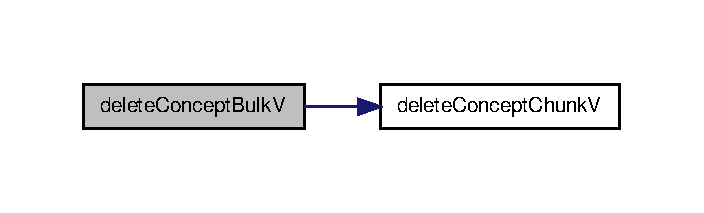
\includegraphics[width=338pt]{vector_2private_8h_aa2cf22779998982c65e3762c7e2c2c84_cgraph}
\end{center}
\end{figure}


\hypertarget{vector_2private_8h_afd9305761d657be7c21fb81e82d72a42}{\index{vector/private.\-h@{vector/private.\-h}!delete\-Concept\-Chunk\-V@{delete\-Concept\-Chunk\-V}}
\index{delete\-Concept\-Chunk\-V@{delete\-Concept\-Chunk\-V}!vector/private.h@{vector/private.\-h}}
\subsubsection[{delete\-Concept\-Chunk\-V}]{\setlength{\rightskip}{0pt plus 5cm}void {\bf delete\-Concept\-Chunk\-V} (
\begin{DoxyParamCaption}
\item[{{\bf my\-Formal\-Concept\-Intent\-Chunk\-V} $\ast$$\ast$}]{c}
\end{DoxyParamCaption}
)}}\label{vector_2private_8h_afd9305761d657be7c21fb81e82d72a42}


deletes a concept chunk object and sets its pointer to zero 


\begin{DoxyParams}{\-Parameters}
{\em c} & pointer to the concept chunk to be deleted \\
\hline
\end{DoxyParams}


\-Definition at line 534 of file fca\-V.\-c.



\-References \-R\-E\-T\-U\-R\-N\-\_\-\-I\-F\-\_\-\-Z\-E\-R\-O.



\-Referenced by delete\-Concept\-Bulk\-V().


\begin{DoxyCode}
{
    RETURN_IF_ZERO(c);
    RETURN_IF_ZERO(*c);

    free((*c)->incidence);

    free(*c);
    *c = 0;
}
\end{DoxyCode}
\hypertarget{vector_2private_8h_a55d40e1b5169e4466d00cb930c67e0ef}{\index{vector/private.\-h@{vector/private.\-h}!intent\-Cmp\-V@{intent\-Cmp\-V}}
\index{intent\-Cmp\-V@{intent\-Cmp\-V}!vector/private.h@{vector/private.\-h}}
\subsubsection[{intent\-Cmp\-V}]{\setlength{\rightskip}{0pt plus 5cm}int {\bf intent\-Cmp\-V} (
\begin{DoxyParamCaption}
\item[{size\-\_\-t}]{attributes, }
\item[{const {\bf \-Incidence\-Vector}}]{minus, }
\item[{const {\bf \-Incidence\-Vector}}]{plus}
\end{DoxyParamCaption}
)}}\label{vector_2private_8h_a55d40e1b5169e4466d00cb930c67e0ef}


compare two intent vectors 


\begin{DoxyParams}{\-Parameters}
{\em attributes} & attribute count \\
\hline
{\em minus} & \char`\"{}left\char`\"{} operand \\
\hline
{\em plus} & \char`\"{}right\char`\"{} operand \\
\hline
\end{DoxyParams}
\begin{DoxyReturn}{\-Returns}
-\/1 if minus is bigger, 1 if plus is bigger, 0 if minus and plus is the same 
\end{DoxyReturn}
in this case, \hyperlink{vector_2macros_8h_ad12dce0a7bf9d908b172a28155b3d261}{\-O\-F\-F\-S\-E\-T(attributes)} == \-O\-F\-F\-S\-E\-T(attributes-\/1)

we only check the lower bits 0 through (attributes-\/1)

\-E\-L\-S\-E\-: attributes has 64 as factor, so we have done all necessary comparisons in the first loop.

\-Definition at line 464 of file fca\-V.\-c.



\-References \-B\-I\-T\-N\-B\-R, \-C\-R\-I\-M\-P\-V\-A\-L\-U\-E, and \-O\-F\-F\-S\-E\-T.



\-Referenced by next\-Closure\-V\-X1().


\begin{DoxyCode}
{
    for (size_t var = 0; var < OFFSET(attributes); ++var)
    {
        if (minus[var] > plus[var])
            return -1;
        if (plus[var] > minus[var])
            return 1;
    }

    if (BITNBR(attributes))
    {
        uint64_t l, r;

        l = minus[OFFSET(attributes)] & CRIMPVALUE(attributes-1);
        r = plus[OFFSET(attributes)] & CRIMPVALUE(attributes-1);

        if (l > r)
            return -1;

        if (r > l)
            return 1;
    }
    return 0;
}
\end{DoxyCode}
\hypertarget{vector_2private_8h_a90151fdf1b3ef3201deb2e1ab752729d}{\index{vector/private.\-h@{vector/private.\-h}!new\-Concept\-Bulk\-From\-Context\-V@{new\-Concept\-Bulk\-From\-Context\-V}}
\index{new\-Concept\-Bulk\-From\-Context\-V@{new\-Concept\-Bulk\-From\-Context\-V}!vector/private.h@{vector/private.\-h}}
\subsubsection[{new\-Concept\-Bulk\-From\-Context\-V}]{\setlength{\rightskip}{0pt plus 5cm}{\bf \-Formal\-Concept\-Intent\-Bulk\-List\-V} {\bf new\-Concept\-Bulk\-From\-Context\-V} (
\begin{DoxyParamCaption}
\item[{{\bf \-Formal\-Context\-V}}]{ctx}
\end{DoxyParamCaption}
)}}\label{vector_2private_8h_a90151fdf1b3ef3201deb2e1ab752729d}


creates a new formal concept intent chunk and fills it with the intents of all formal concepts in the concept lattice of ctx, using next closure algorithm 


\begin{DoxyParams}{\-Parameters}
{\em ctx} & formal context \\
\hline
\end{DoxyParams}
\begin{DoxyReturn}{\-Returns}
concept intents 
\end{DoxyReturn}
calculate the bottom intent of the concept lattice, i.\-e. \{\}''

add the bottom element of the concept lattice (a concept lattice is never empty)

begin of next\-Closure function iteration

we found the next intent

continue with \-Y for \-M

do the next\-Closure

free up memory

\-Definition at line 573 of file fca\-V.\-c.



\-References add\-Concept\-To\-Bulk\-V(), \-C\-L\-E\-A\-R\-V, close\-Intent\-V(), \-C\-R\-I\-M\-P\-V\-A\-L\-U\-E, \-C\-R\-O\-S\-S\-V, \-I\-N\-C\-I\-D\-E\-S\-V, new\-Concept\-Bulk\-V(), \-O\-F\-F\-S\-E\-T, and \-R\-E\-T\-U\-R\-N\-\_\-\-Z\-E\-R\-O\-\_\-\-I\-F\-\_\-\-Z\-E\-R\-O.


\begin{DoxyCode}
{
    RETURN_ZERO_IF_ZERO(ctx);

    myFormalContextV * restrict c;
    c = (myFormalContextV*) ctx;

    IncidenceVector restrict M;
    IncidenceVector restrict Y;

#pragma GCC diagnostic push
#pragma GCC diagnostic ignored "-Wsign-conversion"

    Y = calloc(c->width, sizeof(uint64_t));
    M = malloc(c->width * sizeof(uint64_t));

#pragma GCC diagnostic pop

    closeIntentV(ctx, Y, M);

    FormalConceptIntentBulkListV root;
    FormalConceptIntentBulkListV last;

    root = newConceptBulkV(c->attributes);

    last = addConceptToBulkV(root, M);

    nextClosure:

    for (size_t i = c->attributes; i > 0;)
    {
        --i;

        if (!INCIDESV(M,i))
        {
            CROSSV(M, i);
            closeIntentV(ctx, M, Y);

            int good;
            good = 1;

            for (unsigned int j = 0; j < OFFSET(i); ++j)
            {
                if (Y[j] & (~(M[j])))
                {
                    good = 0;
                    break;
                }
            }
            if (good)
            {
                if (Y[OFFSET(i)] & (~M[OFFSET(i)]) & CRIMPVALUE(i))
                {
                    good = 0;
                }
            }

            if (good)
            {

                last = addConceptToBulkV(last, Y);

                IncidenceVector DELTA;
                DELTA = M;
                M = Y;
                Y = DELTA;
                goto nextClosure;
            }
        }

        CLEARV(M, i);
    }

    free(M);
    free(Y);

    return root;
}
\end{DoxyCode}


\-Here is the call graph for this function\-:\nopagebreak
\begin{figure}[H]
\begin{center}
\leavevmode
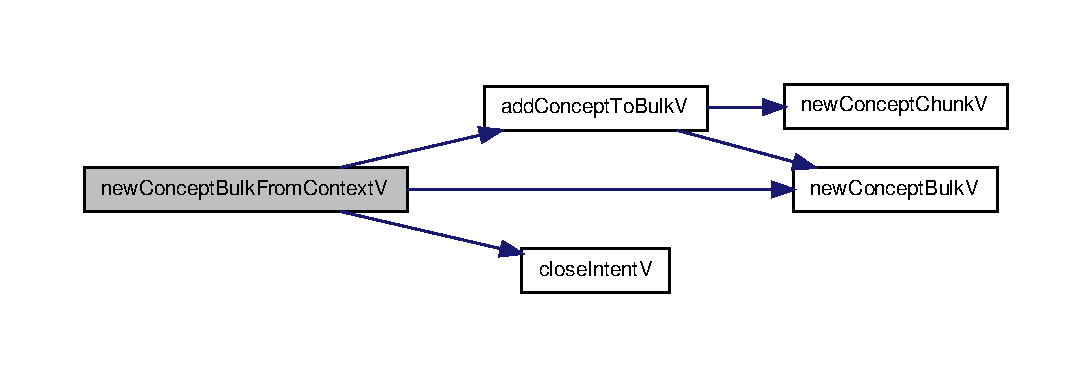
\includegraphics[width=350pt]{vector_2private_8h_a90151fdf1b3ef3201deb2e1ab752729d_cgraph}
\end{center}
\end{figure}


\hypertarget{vector_2private_8h_abda612c4305c29a37b6501e18d94ebc5}{\index{vector/private.\-h@{vector/private.\-h}!new\-Concept\-Bulk\-V@{new\-Concept\-Bulk\-V}}
\index{new\-Concept\-Bulk\-V@{new\-Concept\-Bulk\-V}!vector/private.h@{vector/private.\-h}}
\subsubsection[{new\-Concept\-Bulk\-V}]{\setlength{\rightskip}{0pt plus 5cm}{\bf \-Formal\-Concept\-Intent\-Bulk\-List\-V} {\bf new\-Concept\-Bulk\-V} (
\begin{DoxyParamCaption}
\item[{size\-\_\-t}]{attributes}
\end{DoxyParamCaption}
)}}\label{vector_2private_8h_abda612c4305c29a37b6501e18d94ebc5}


creates a new formal concept intent bulk list 


\begin{DoxyParams}{\-Parameters}
{\em attributes} & number of attributes of the concept intents \\
\hline
\end{DoxyParams}
\begin{DoxyReturn}{\-Returns}
new formal concept intent bulk list's first node 
\end{DoxyReturn}


\-Definition at line 552 of file fca\-V.\-c.



\-References s\-Formal\-Concept\-Intent\-Bulk\-Node\-V\-::attributes, \-B\-U\-L\-K\-S\-I\-Z\-E\-V, s\-Formal\-Concept\-Intent\-Bulk\-Node\-V\-::chunks, s\-Formal\-Concept\-Intent\-Bulk\-Node\-V\-::next, s\-Formal\-Concept\-Intent\-Bulk\-Node\-V\-::size, \-W\-I\-D\-T\-H, and s\-Formal\-Concept\-Intent\-Bulk\-Node\-V\-::width.



\-Referenced by add\-Concept\-To\-Bulk\-V(), new\-Concept\-Bulk\-From\-Context\-V(), and next\-Closure\-V\-X1().


\begin{DoxyCode}
{
    FormalConceptIntentBulkListV l;
    l = malloc(sizeof(struct sFormalConceptIntentBulkNodeV));

    l->attributes = attributes;
    l->width = WIDTH(attributes);
    l->size = 0;
    l->chunks = calloc(BULKSIZEV, sizeof(myFormalConceptIntentChunkV*));
    l->next = 0;
    return l;
}
\end{DoxyCode}
\hypertarget{vector_2private_8h_ab5c9a71c810ad1eeeb5f8ff78d77d899}{\index{vector/private.\-h@{vector/private.\-h}!new\-Concept\-Chunk\-V@{new\-Concept\-Chunk\-V}}
\index{new\-Concept\-Chunk\-V@{new\-Concept\-Chunk\-V}!vector/private.h@{vector/private.\-h}}
\subsubsection[{new\-Concept\-Chunk\-V}]{\setlength{\rightskip}{0pt plus 5cm}{\bf my\-Formal\-Concept\-Intent\-Chunk\-V}$\ast$ {\bf new\-Concept\-Chunk\-V} (
\begin{DoxyParamCaption}
\item[{size\-\_\-t}]{attributes}
\end{DoxyParamCaption}
)}}\label{vector_2private_8h_ab5c9a71c810ad1eeeb5f8ff78d77d899}


create a new formal concept chunk 


\begin{DoxyParams}{\-Parameters}
{\em attributes} & number of attributes of the hosting formal context \\
\hline
\end{DoxyParams}
\begin{DoxyReturn}{\-Returns}
a new concept chunk object 
\end{DoxyReturn}


\-Definition at line 507 of file fca\-V.\-c.



\-References smy\-Formal\-Concept\-Intent\-Chunk\-V\-::attributes, \-C\-H\-U\-N\-K\-S\-I\-Z\-E\-V, smy\-Formal\-Concept\-Intent\-Chunk\-V\-::incidence, smy\-Formal\-Concept\-Intent\-Chunk\-V\-::size, \-W\-I\-D\-T\-H, and smy\-Formal\-Concept\-Intent\-Chunk\-V\-::width.



\-Referenced by add\-Concept\-To\-Bulk\-V().


\begin{DoxyCode}
{

    myFormalConceptIntentChunkV *c;

    c = malloc(sizeof(myFormalConceptIntentChunkV));

    c->attributes = attributes;
    c->width = WIDTH(attributes);
    c->size = 0;

#pragma GCC diagnostic push
#pragma GCC diagnostic ignored "-Wsign-conversion"

    c->incidence = calloc(c->width * CHUNKSIZEV, sizeof(uint64_t));

#pragma GCC diagnostic pop

    return c;
}
\end{DoxyCode}
\hypertarget{vector_2private_8h_a858241e44987c35c2ae688f2797f2a30}{\index{vector/private.\-h@{vector/private.\-h}!next\-Closure\-V\-X@{next\-Closure\-V\-X}}
\index{next\-Closure\-V\-X@{next\-Closure\-V\-X}!vector/private.h@{vector/private.\-h}}
\subsubsection[{next\-Closure\-V\-X}]{\setlength{\rightskip}{0pt plus 5cm}{\bf \-Formal\-Concept\-Intent\-Bulk\-List\-V} {\bf next\-Closure\-V\-X} (
\begin{DoxyParamCaption}
\item[{{\bf \-Formal\-Context\-V}}]{ctx}
\end{DoxyParamCaption}
)}}\label{vector_2private_8h_a858241e44987c35c2ae688f2797f2a30}


creates a new formal concept intent chunk and fills it with the intents of all formal concepts in the concept lattice of ctx, using a parallel next closure algorithm with up to 8 threads 


\begin{DoxyParams}{\-Parameters}
{\em ctx} & formal context \\
\hline
\end{DoxyParams}
\begin{DoxyReturn}{\-Returns}
concept intents 
\end{DoxyReturn}


\-Definition at line 199 of file fca\-Vnext\-Closure\-X.\-c.



\-References smy\-Formal\-Context\-V\-::attributes, call\-Next\-Closure\-V\-X1(), \-C\-R\-O\-S\-S\-V, snext\-Closure\-V\-X1\-Params\-::ctx, s\-Formal\-Concept\-Intent\-Bulk\-Node\-V\-::next, next\-Closure\-V\-X1(), \-R\-E\-T\-U\-R\-N\-\_\-\-Z\-E\-R\-O\-\_\-\-I\-F\-\_\-\-Z\-E\-R\-O, snext\-Closure\-V\-X1\-Params\-::r\-Val, snext\-Closure\-V\-X1\-Params\-::start, snext\-Closure\-V\-X1\-Params\-::stop, and smy\-Formal\-Context\-V\-::width.


\begin{DoxyCode}
{
    RETURN_ZERO_IF_ZERO(ctx);

    myFormalContextV *c;
    c = (myFormalContextV*) ctx;

    size_t N;

    N = 1;

    if (c->attributes >= 3)
        N = 8;
    else if (c->attributes >= 2)
        N = 4;
    else if (c->attributes >= 1)
        N = 2;

    if (N < 2)
        return nextClosureVX1(ctx, 0, 0);

    IncidenceVector bounds;
    bounds = calloc(c->width * (N - 1), sizeof(uint64_t));

    if (N == 2)
    {
        CROSSV(bounds, 0);
    }
    else if (N == 4)
    {
        CROSSV(bounds, 1); //01

        CROSSV(bounds + c->width, 0); //10

        CROSSV(bounds + c->width * 2, 1); //11
        CROSSV(bounds + c->width * 2, 0);
    }
    else if (N == 8)
    {
        CROSSV(bounds, 2); // 001

        CROSSV(bounds + c->width, 1); //010

        CROSSV(bounds + c->width * 2, 2); //011
        CROSSV(bounds + c->width * 2, 1);

        CROSSV(bounds + c->width * 3, 0); //100

        CROSSV(bounds + c->width * 4, 0); //101
        CROSSV(bounds + c->width * 4, 2);

        CROSSV(bounds + c->width * 5, 1); //110
        CROSSV(bounds + c->width * 5, 0);

        CROSSV(bounds + c->width * 6, 0); //111
        CROSSV(bounds + c->width * 6, 1);
        CROSSV(bounds + c->width * 6, 2);
    }

//  for (int i = 0; i < N - 1; ++i)
//  {
//      printf("BOUND %16llx\n", *(bounds + i *
       c->width)&CRIMPVALUE(c->attributes-1));
//      if (i > 0)
//          printf("CMP %d\n",
//                  intentCmpV(c->attributes, bounds + (i - 1) * c->width,
//                          bounds + i * c->width));
//  }


    nextClosureVX1Params chunks;
    chunks = malloc(N * sizeof(struct snextClosureVX1Params));

    pthread_t *threads;
    threads = malloc(N * sizeof(pthread_t));

    for (size_t i = 0; i < N; ++i)
    {
        chunks[i].ctx = ctx;
        if (i > 0)
            chunks[i].start = (bounds + c->width * (i - 1));
        else
            chunks[i].start = 0;

        if (i < N - 1)
            chunks[i].stop = (bounds + c->width * (i));
        else
            chunks[i].stop = 0;
    }

    for (size_t i = 0; i < N; ++i)
    {
        pthread_create(&threads[i], 0, callNextClosureVX1, (void*) &chunks[i]);
    }

    for (size_t i = 0; i < N; ++i)
    {
        pthread_join(threads[i], 0);
    }

//  for (size_t i = 0; i < N; ++i)
//  {
//      printf("%zu thread: counts %zu\n", i,
//              countConceptsInBulkV(chunks[i].rVal));
//  }

    FormalConceptIntentBulkListV root;
    FormalConceptIntentBulkListV last;

    root = chunks[0].rVal;
    last = root;

    for (size_t var = 1; var < N; ++var)
    {

        while (last->next)
            last = last->next;

        last->next = chunks[var].rVal;
    }

    free(bounds);
    free(chunks);

    return root;
}
\end{DoxyCode}


\-Here is the call graph for this function\-:\nopagebreak
\begin{figure}[H]
\begin{center}
\leavevmode
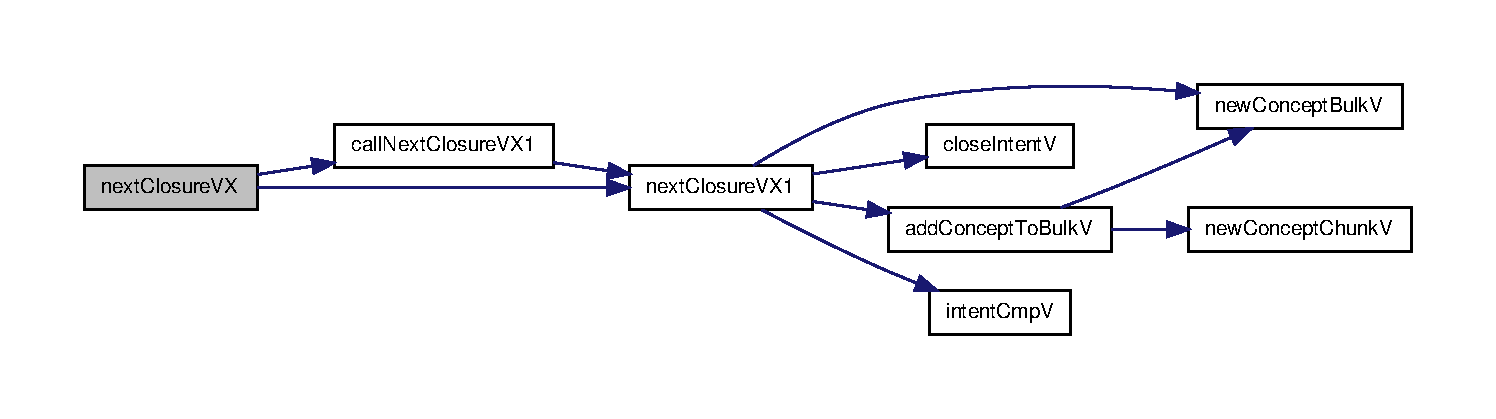
\includegraphics[width=350pt]{vector_2private_8h_a858241e44987c35c2ae688f2797f2a30_cgraph}
\end{center}
\end{figure}


\hypertarget{vector_2private_8h_a8ee9a9ab122e4e5e8c5148ef759172f2}{\index{vector/private.\-h@{vector/private.\-h}!next\-Closure\-V\-X1@{next\-Closure\-V\-X1}}
\index{next\-Closure\-V\-X1@{next\-Closure\-V\-X1}!vector/private.h@{vector/private.\-h}}
\subsubsection[{next\-Closure\-V\-X1}]{\setlength{\rightskip}{0pt plus 5cm}{\bf \-Formal\-Concept\-Intent\-Bulk\-List\-V} {\bf next\-Closure\-V\-X1} (
\begin{DoxyParamCaption}
\item[{{\bf \-Formal\-Context\-V}}]{ctx, }
\item[{const {\bf \-Incidence\-Vector} restrict}]{start, }
\item[{const {\bf \-Incidence\-Vector} restrict}]{stop}
\end{DoxyParamCaption}
)}}\label{vector_2private_8h_a8ee9a9ab122e4e5e8c5148ef759172f2}


creates a new formal concept intent chunk and fills it with the intents of all formal concepts in the concept lattice of ctx, using next closure algorithm, that are in a given lexicographic interval of the powerset 


\begin{DoxyParams}{\-Parameters}
{\em ctx} & formal context \\
\hline
{\em start} & first attribute vector (not included if it is a concept intent) if this is zero, start with \-M=\{\}, in this case, we add the bottom concept in case of \-M''==\{\} \\
\hline
{\em stop} & last attribute vector, or zero to continue until the end \\
\hline
\end{DoxyParams}
\begin{DoxyReturn}{\-Returns}
concept intents between (start, stop\mbox{]} 
\end{DoxyReturn}
calculate the bottom intent of the concept lattice, i.\-e. \{\}''

add the bottom element of the concept lattice (a concept lattice is never empty)

begin of next\-Closure function iteration

check whether we are still in range

the (pseudo)intent \-Y is bigger than stop

we found the next intent

continue with \-Y for \-M

do the next\-Closure

free up memory

\-Definition at line 47 of file fca\-Vnext\-Closure\-X.\-c.



\-References add\-Concept\-To\-Bulk\-V(), \-C\-L\-E\-A\-R\-V, close\-Intent\-V(), \-C\-R\-I\-M\-P\-V\-A\-L\-U\-E, \-C\-R\-O\-S\-S\-V, \-I\-N\-C\-I\-D\-E\-S\-V, intent\-Cmp\-V(), new\-Concept\-Bulk\-V(), \-O\-F\-F\-S\-E\-T, and \-R\-E\-T\-U\-R\-N\-\_\-\-Z\-E\-R\-O\-\_\-\-I\-F\-\_\-\-Z\-E\-R\-O.



\-Referenced by call\-Next\-Closure\-V\-X1(), and next\-Closure\-V\-X().


\begin{DoxyCode}
{
    RETURN_ZERO_IF_ZERO(ctx);

    myFormalContextV * restrict c;
    c = (myFormalContextV*) ctx;

    IncidenceVector restrict M;
    IncidenceVector restrict Y;

    Y = calloc(c->width, sizeof(uint64_t));
    M = malloc(c->width * sizeof(uint64_t));

    FormalConceptIntentBulkListV root;
    FormalConceptIntentBulkListV last;

    root = newConceptBulkV(c->attributes);

    if (start)
    {
        memcpy(M, start, c->width * sizeof(uint64_t));

        last = root;

    }
    else
    {

        closeIntentV(ctx, Y, M);

        last = addConceptToBulkV(root, M);
    }

    nextClosure:

    for (size_t i = c->attributes; i > 0;)
    {
        --i;

        if (!INCIDESV(M,i))
        {
            CROSSV(M, i);
            closeIntentV(ctx, M, Y);

            int good;
            good = 1;

            for (unsigned int j = 0; j < OFFSET(i); ++j)
            {
                if (Y[j] & (~(M[j])))
                {
                    good = 0;
                    break;
                }
            }
            if (good)
            {
                if (Y[OFFSET(i)] & (~M[OFFSET(i)]) & CRIMPVALUE(i))
                {
                    good = 0;
                }
            }

            if (good)
            {
                if (stop)
                {
                    if (intentCmpV(c->attributes, Y, stop) < 0)
                    {
                        goto gracefulReturn;
                    }
                }

                last = addConceptToBulkV(last, Y);

                IncidenceVector DELTA;
                DELTA = M;
                M = Y;
                Y = DELTA;
                goto nextClosure;
            }
        }

        CLEARV(M, i);
    }

    gracefulReturn:
    free(M);
    free(Y);

    return root;
}
\end{DoxyCode}


\-Here is the call graph for this function\-:\nopagebreak
\begin{figure}[H]
\begin{center}
\leavevmode
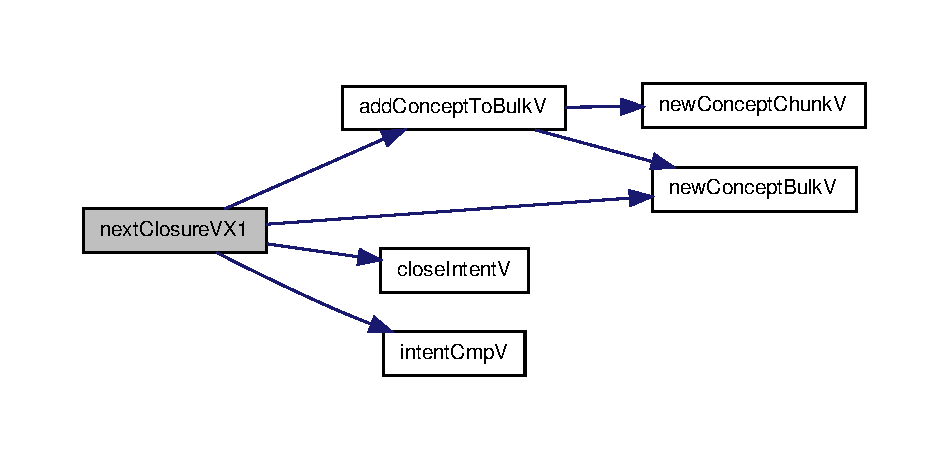
\includegraphics[width=350pt]{vector_2private_8h_a8ee9a9ab122e4e5e8c5148ef759172f2_cgraph}
\end{center}
\end{figure}


\hypertarget{vector_2private_8h_ac1443261c57cc1d3db9361c188cd9c96}{\index{vector/private.\-h@{vector/private.\-h}!write\-Concepts\-To\-File\-V@{write\-Concepts\-To\-File\-V}}
\index{write\-Concepts\-To\-File\-V@{write\-Concepts\-To\-File\-V}!vector/private.h@{vector/private.\-h}}
\subsubsection[{write\-Concepts\-To\-File\-V}]{\setlength{\rightskip}{0pt plus 5cm}void {\bf write\-Concepts\-To\-File\-V} (
\begin{DoxyParamCaption}
\item[{{\bf \-Formal\-Context\-V}}]{ctx, }
\item[{{\bf \-Formal\-Concept\-Intent\-Bulk\-List\-V}}]{root, }
\item[{const char $\ast$}]{filename}
\end{DoxyParamCaption}
)}}\label{vector_2private_8h_ac1443261c57cc1d3db9361c188cd9c96}


write a list of concept intents into a .cxt file 


\begin{DoxyParams}{\-Parameters}
{\em ctx} & formal context (or 0, is used for attribute names) \\
\hline
{\em root} & the first node of the formal concept intent bulk \\
\hline
{\em filename} & output file name (.cxt) \\
\hline
\end{DoxyParams}


\-Definition at line 684 of file fca\-V.\-c.



\-References smy\-Formal\-Context\-V\-::attribute\-Names, smy\-Formal\-Context\-V\-::attributes, s\-Formal\-Concept\-Intent\-Bulk\-Node\-V\-::attributes, s\-Formal\-Concept\-Intent\-Bulk\-Node\-V\-::chunks, count\-Concepts\-In\-Bulk\-V(), \-I\-N\-C\-I\-D\-E\-S\-V, s\-Formal\-Concept\-Intent\-Bulk\-Node\-V\-::next, \-R\-E\-T\-U\-R\-N\-\_\-\-I\-F\-\_\-\-Z\-E\-R\-O, \-R\-O\-W, smy\-Formal\-Concept\-Intent\-Chunk\-V\-::size, s\-Formal\-Concept\-Intent\-Bulk\-Node\-V\-::size, and \-W\-A\-R\-N\-\_\-\-I\-F\-\_\-\-U\-N\-E\-Q\-U\-A\-L\-\_\-\-D\-O.


\begin{DoxyCode}
{
    RETURN_IF_ZERO(root);

    myFormalContextV* c;

    if (ctx != 0)
    {
        c = (myFormalContextV*) ctx;

        WARN_IF_UNEQUAL_DO(c->attributes, root->attributes, c = 0);
    }
    else
    {
        c = 0;
    }

    RETURN_IF_ZERO(filename);

    FILE* file;
    file = fopen(filename, "w");

    RETURN_IF_ZERO(file);

    size_t objects;
    objects = countConceptsInBulkV(root);

    fprintf(file, "B\n\n%zu\n%zu\n\n", objects, root->attributes);

    for (size_t var = 0; var < objects; ++var)
    {
        fprintf(file, "C%8zu\n", (var + 1));
    }

    if (c != 0)
    {
        for (size_t var = 0; var < c->attributes; ++var)
        {
            fputs(c->attributeNames[var], file);
            fputs("\n", file);
        }
    }
    else
    {
        for (size_t var = 0; var < root->attributes; ++var)
        {
            fprintf(file, "m%8zu\n", (var + 1));
        }
    }

    for (; root != 0; root = root->next)
    {
        for (size_t chunk = 0; chunk < root->size; ++chunk)
        {
            for (size_t g = 0; g < root->chunks[chunk]->size; ++g)
            {
                for (size_t m = 0; m < root->attributes; ++m)
                {
                    if (INCIDESV(ROW(g, root->chunks[chunk]), m))
                        fputs("X", file);
                    else
                        fputs(".", file);
                }
                fputs("\n", file);
            }
        }
    }

    fclose(file);
}
\end{DoxyCode}


\-Here is the call graph for this function\-:\nopagebreak
\begin{figure}[H]
\begin{center}
\leavevmode
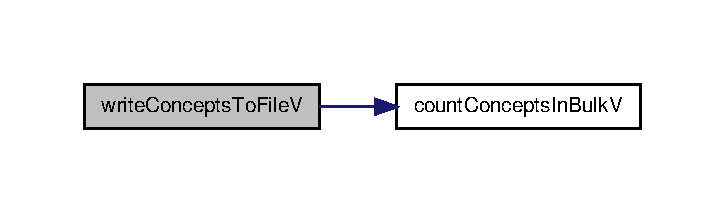
\includegraphics[width=348pt]{vector_2private_8h_ac1443261c57cc1d3db9361c188cd9c96_cgraph}
\end{center}
\end{figure}



\hypertarget{easy_2structs_8h}{\section{src/fca/easy/structs.h \-File \-Reference}
\label{easy_2structs_8h}\index{src/fca/easy/structs.\-h@{src/fca/easy/structs.\-h}}
}
\-This graph shows which files directly or indirectly include this file\-:
\nopagebreak
\begin{figure}[H]
\begin{center}
\leavevmode
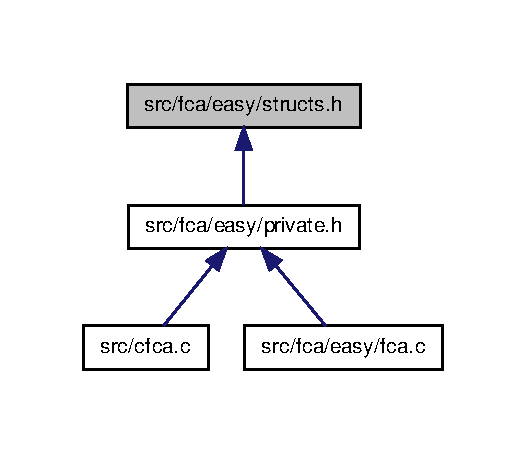
\includegraphics[width=350pt]{easy_2structs_8h__dep__incl}
\end{center}
\end{figure}
\subsection*{\-Data \-Structures}
\begin{DoxyCompactItemize}
\item 
struct \hyperlink{structsmyFormalContext}{smy\-Formal\-Context}
\begin{DoxyCompactList}\small\item\em each formal context has a finite number of objects and attributes, which may have names (though we do not require them to be unique or given), and an incidence relation which is represented by an objects×attributes-\/\-Incidence\-Cell matrix \end{DoxyCompactList}\item 
struct \hyperlink{structsmyFormalConceptIntentChunk}{smy\-Formal\-Concept\-Intent\-Chunk}
\begin{DoxyCompactList}\small\item\em \-A chunk of at most \-C\-H\-U\-N\-K\-S\-I\-Z\-E formal concept intents. \end{DoxyCompactList}\item 
struct \hyperlink{structsFormalConceptIntentBulkNode}{s\-Formal\-Concept\-Intent\-Bulk\-Node}
\begin{DoxyCompactList}\small\item\em a node of a single linked list of concept chunks. \end{DoxyCompactList}\end{DoxyCompactItemize}
\subsection*{\-Defines}
\begin{DoxyCompactItemize}
\item 
\#define \hyperlink{easy_2structs_8h_a239bebe1697b474e6f84945e9fb9faee}{\-C\-H\-U\-N\-K\-S\-I\-Z\-E}~(64)
\begin{DoxyCompactList}\small\item\em \hyperlink{easy_2structs_8h}{easy/structs.\-h}, (c) 2013, \-Immanuel \-Albrecht; \-Dresden \-University of \-Technology, \-Professur für die \-Psychologie des \-Lernen und \-Lehrens \end{DoxyCompactList}\item 
\#define \hyperlink{easy_2structs_8h_a9bd2a644fe274f91e81aae543b9901c6}{\-B\-U\-L\-K\-S\-I\-Z\-E}~(1024)
\begin{DoxyCompactList}\small\item\em size of chunks per bulk \end{DoxyCompactList}\item 
\#define \hyperlink{easy_2structs_8h_a2129a125f29c4f6de8a39cc771176482}{\-I\-N\-P\-U\-T\-B\-U\-F\-F\-E\-R\-S\-I\-Z\-E}~(1024)
\begin{DoxyCompactList}\small\item\em maximal (initial) size of a line (getline will resize buffers if necessary) (including delimiter) \end{DoxyCompactList}\end{DoxyCompactItemize}
\subsection*{\-Typedefs}
\begin{DoxyCompactItemize}
\item 
typedef struct \hyperlink{structsmyFormalContext}{smy\-Formal\-Context} \hyperlink{easy_2structs_8h_a35fe69cf5a1b22acf807e7aa13a6d270}{my\-Formal\-Context}
\begin{DoxyCompactList}\small\item\em each formal context has a finite number of objects and attributes, which may have names (though we do not require them to be unique or given), and an incidence relation which is represented by an objects×attributes-\/\-Incidence\-Cell matrix \end{DoxyCompactList}\item 
typedef struct \*
\hyperlink{structsmyFormalConceptIntentChunk}{smy\-Formal\-Concept\-Intent\-Chunk} \hyperlink{easy_2structs_8h_ae552e1b13988c8c4ca0ab8f8a3e60f96}{my\-Formal\-Concept\-Intent\-Chunk}
\begin{DoxyCompactList}\small\item\em \-A chunk of at most \-C\-H\-U\-N\-K\-S\-I\-Z\-E formal concept intents. \end{DoxyCompactList}\item 
typedef struct \*
\hyperlink{structsFormalConceptIntentBulkNode}{s\-Formal\-Concept\-Intent\-Bulk\-Node} $\ast$ \hyperlink{easy_2structs_8h_a6c7fd90fd34d9ca52fedd96a01dd3566}{\-Formal\-Concept\-Intent\-Bulk\-List}
\begin{DoxyCompactList}\small\item\em a node of a single linked list of concept chunks. \end{DoxyCompactList}\end{DoxyCompactItemize}


\subsection{\-Define \-Documentation}
\hypertarget{easy_2structs_8h_a9bd2a644fe274f91e81aae543b9901c6}{\index{easy/structs.\-h@{easy/structs.\-h}!\-B\-U\-L\-K\-S\-I\-Z\-E@{\-B\-U\-L\-K\-S\-I\-Z\-E}}
\index{\-B\-U\-L\-K\-S\-I\-Z\-E@{\-B\-U\-L\-K\-S\-I\-Z\-E}!easy/structs.h@{easy/structs.\-h}}
\subsubsection[{\-B\-U\-L\-K\-S\-I\-Z\-E}]{\setlength{\rightskip}{0pt plus 5cm}\#define {\bf \-B\-U\-L\-K\-S\-I\-Z\-E}~(1024)}}\label{easy_2structs_8h_a9bd2a644fe274f91e81aae543b9901c6}


size of chunks per bulk 



\-Definition at line 35 of file structs.\-h.



\-Referenced by add\-Concept\-To\-Bulk(), and new\-Concept\-Bulk().

\hypertarget{easy_2structs_8h_a239bebe1697b474e6f84945e9fb9faee}{\index{easy/structs.\-h@{easy/structs.\-h}!\-C\-H\-U\-N\-K\-S\-I\-Z\-E@{\-C\-H\-U\-N\-K\-S\-I\-Z\-E}}
\index{\-C\-H\-U\-N\-K\-S\-I\-Z\-E@{\-C\-H\-U\-N\-K\-S\-I\-Z\-E}!easy/structs.h@{easy/structs.\-h}}
\subsubsection[{\-C\-H\-U\-N\-K\-S\-I\-Z\-E}]{\setlength{\rightskip}{0pt plus 5cm}\#define {\bf \-C\-H\-U\-N\-K\-S\-I\-Z\-E}~(64)}}\label{easy_2structs_8h_a239bebe1697b474e6f84945e9fb9faee}


\hyperlink{easy_2structs_8h}{easy/structs.\-h}, (c) 2013, \-Immanuel \-Albrecht; \-Dresden \-University of \-Technology, \-Professur für die \-Psychologie des \-Lernen und \-Lehrens 

\-This program is free software\-: you can redistribute it and/or modify it under the terms of the \-G\-N\-U \-General \-Public \-License as published by the \-Free \-Software \-Foundation, either version 3 of the \-License, or (at your option) any later version.

\-This program is distributed in the hope that it will be useful, but \-W\-I\-T\-H\-O\-U\-T \-A\-N\-Y \-W\-A\-R\-R\-A\-N\-T\-Y; without even the implied warranty of \-M\-E\-R\-C\-H\-A\-N\-T\-A\-B\-I\-L\-I\-T\-Y or \-F\-I\-T\-N\-E\-S\-S \-F\-O\-R \-A \-P\-A\-R\-T\-I\-C\-U\-L\-A\-R \-P\-U\-R\-P\-O\-S\-E. \-See the \-G\-N\-U \-General \-Public \-License for more details.

\-You should have received a copy of the \-G\-N\-U \-General \-Public \-License along with this program. \-If not, see $<$\href{http://www.gnu.org/licenses/}{\tt http\-://www.\-gnu.\-org/licenses/}$>$.

size of a chunk of concepts 

\-Definition at line 27 of file structs.\-h.



\-Referenced by add\-Concept\-To\-Bulk(), count\-Concepts\-In\-Bulk(), and new\-Concept\-Chunk().

\hypertarget{easy_2structs_8h_a2129a125f29c4f6de8a39cc771176482}{\index{easy/structs.\-h@{easy/structs.\-h}!\-I\-N\-P\-U\-T\-B\-U\-F\-F\-E\-R\-S\-I\-Z\-E@{\-I\-N\-P\-U\-T\-B\-U\-F\-F\-E\-R\-S\-I\-Z\-E}}
\index{\-I\-N\-P\-U\-T\-B\-U\-F\-F\-E\-R\-S\-I\-Z\-E@{\-I\-N\-P\-U\-T\-B\-U\-F\-F\-E\-R\-S\-I\-Z\-E}!easy/structs.h@{easy/structs.\-h}}
\subsubsection[{\-I\-N\-P\-U\-T\-B\-U\-F\-F\-E\-R\-S\-I\-Z\-E}]{\setlength{\rightskip}{0pt plus 5cm}\#define {\bf \-I\-N\-P\-U\-T\-B\-U\-F\-F\-E\-R\-S\-I\-Z\-E}~(1024)}}\label{easy_2structs_8h_a2129a125f29c4f6de8a39cc771176482}


maximal (initial) size of a line (getline will resize buffers if necessary) (including delimiter) 



\-Definition at line 42 of file structs.\-h.



\-Referenced by new\-Formal\-Context\-From\-File(), and new\-Formal\-Context\-From\-File\-V().



\subsection{\-Typedef \-Documentation}
\hypertarget{easy_2structs_8h_a6c7fd90fd34d9ca52fedd96a01dd3566}{\index{easy/structs.\-h@{easy/structs.\-h}!\-Formal\-Concept\-Intent\-Bulk\-List@{\-Formal\-Concept\-Intent\-Bulk\-List}}
\index{\-Formal\-Concept\-Intent\-Bulk\-List@{\-Formal\-Concept\-Intent\-Bulk\-List}!easy/structs.h@{easy/structs.\-h}}
\subsubsection[{\-Formal\-Concept\-Intent\-Bulk\-List}]{\setlength{\rightskip}{0pt plus 5cm}typedef struct {\bf s\-Formal\-Concept\-Intent\-Bulk\-Node}$\ast$  {\bf \-Formal\-Concept\-Intent\-Bulk\-List}}}\label{easy_2structs_8h_a6c7fd90fd34d9ca52fedd96a01dd3566}


a node of a single linked list of concept chunks. 

bulk nodes are filled chunk wise, but a bulk node may have non-\/empty successor nodes even if it is not entire full. \hypertarget{easy_2structs_8h_ae552e1b13988c8c4ca0ab8f8a3e60f96}{\index{easy/structs.\-h@{easy/structs.\-h}!my\-Formal\-Concept\-Intent\-Chunk@{my\-Formal\-Concept\-Intent\-Chunk}}
\index{my\-Formal\-Concept\-Intent\-Chunk@{my\-Formal\-Concept\-Intent\-Chunk}!easy/structs.h@{easy/structs.\-h}}
\subsubsection[{my\-Formal\-Concept\-Intent\-Chunk}]{\setlength{\rightskip}{0pt plus 5cm}typedef struct {\bf smy\-Formal\-Concept\-Intent\-Chunk}  {\bf my\-Formal\-Concept\-Intent\-Chunk}}}\label{easy_2structs_8h_ae552e1b13988c8c4ca0ab8f8a3e60f96}


\-A chunk of at most \-C\-H\-U\-N\-K\-S\-I\-Z\-E formal concept intents. 

\hypertarget{easy_2structs_8h_a35fe69cf5a1b22acf807e7aa13a6d270}{\index{easy/structs.\-h@{easy/structs.\-h}!my\-Formal\-Context@{my\-Formal\-Context}}
\index{my\-Formal\-Context@{my\-Formal\-Context}!easy/structs.h@{easy/structs.\-h}}
\subsubsection[{my\-Formal\-Context}]{\setlength{\rightskip}{0pt plus 5cm}typedef struct {\bf smy\-Formal\-Context}  {\bf my\-Formal\-Context}}}\label{easy_2structs_8h_a35fe69cf5a1b22acf807e7aa13a6d270}


each formal context has a finite number of objects and attributes, which may have names (though we do not require them to be unique or given), and an incidence relation which is represented by an objects×attributes-\/\-Incidence\-Cell matrix 


\hypertarget{vector_2structs_8h}{\section{src/vector/structs.h \-File \-Reference}
\label{vector_2structs_8h}\index{src/vector/structs.\-h@{src/vector/structs.\-h}}
}
\-This graph shows which files directly or indirectly include this file\-:
\nopagebreak
\begin{figure}[H]
\begin{center}
\leavevmode
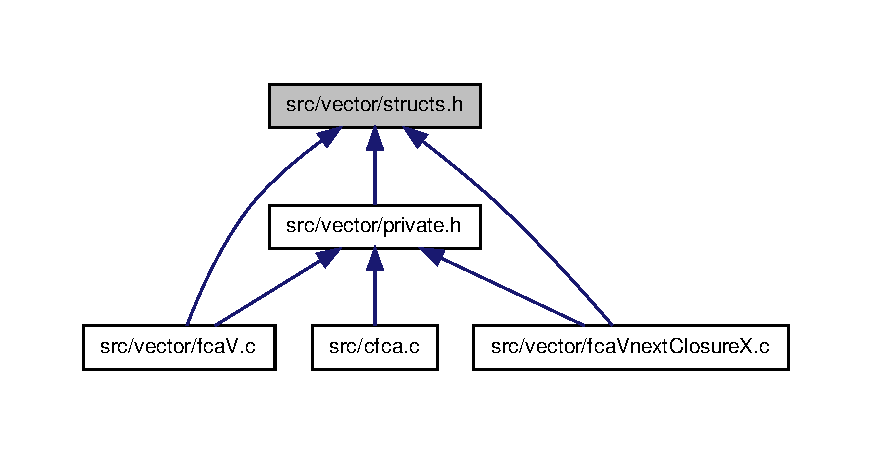
\includegraphics[width=350pt]{vector_2structs_8h__dep__incl}
\end{center}
\end{figure}
\subsection*{\-Data \-Structures}
\begin{DoxyCompactItemize}
\item 
struct \hyperlink{structsmyFormalContextV}{smy\-Formal\-Context\-V}
\begin{DoxyCompactList}\small\item\em each formal context has a finite number of objects and attributes, which may have names (though we do not require them to be unique or given), and an incidence relation which is represented by an objects×attributes-\/\-Incidence\-Cell matrix \end{DoxyCompactList}\item 
struct \hyperlink{structsmyFormalConceptIntentChunkV}{smy\-Formal\-Concept\-Intent\-Chunk\-V}
\begin{DoxyCompactList}\small\item\em \-A chunk of at most \-C\-H\-U\-N\-K\-S\-I\-Z\-E\-V formal concept intent vectors. \end{DoxyCompactList}\item 
struct \hyperlink{structsFormalConceptIntentBulkNodeV}{s\-Formal\-Concept\-Intent\-Bulk\-Node\-V}
\begin{DoxyCompactList}\small\item\em a node of a single linked list of concept chunks. \end{DoxyCompactList}\end{DoxyCompactItemize}
\subsection*{\-Defines}
\begin{DoxyCompactItemize}
\item 
\#define \hyperlink{vector_2structs_8h_aac302242f1cae503941aea3e7c50521f}{\-C\-H\-U\-N\-K\-S\-I\-Z\-E\-V}~(1024)
\begin{DoxyCompactList}\small\item\em \hyperlink{vector_2structs_8h}{vector/structs.\-h}, (c) 2013, \-Immanuel \-Albrecht; \-Dresden \-University of \-Technology, \-Professur für die \-Psychologie des \-Lernen und \-Lehrens \end{DoxyCompactList}\item 
\#define \hyperlink{vector_2structs_8h_a975f482c86513cd75103e7c11d386ee8}{\-B\-U\-L\-K\-S\-I\-Z\-E\-V}~(1024)
\begin{DoxyCompactList}\small\item\em size of chunks per bulk (vector version) \end{DoxyCompactList}\item 
\#define \hyperlink{vector_2structs_8h_a2129a125f29c4f6de8a39cc771176482}{\-I\-N\-P\-U\-T\-B\-U\-F\-F\-E\-R\-S\-I\-Z\-E}~(1024)
\begin{DoxyCompactList}\small\item\em maximal (initial) size of a line (getline will resize buffers if necessary) (including delimiter) \end{DoxyCompactList}\end{DoxyCompactItemize}
\subsection*{\-Typedefs}
\begin{DoxyCompactItemize}
\item 
typedef struct \hyperlink{structsmyFormalContextV}{smy\-Formal\-Context\-V} \hyperlink{vector_2structs_8h_a84718211dcd64835d30f05465ddd2547}{my\-Formal\-Context\-V}
\begin{DoxyCompactList}\small\item\em each formal context has a finite number of objects and attributes, which may have names (though we do not require them to be unique or given), and an incidence relation which is represented by an objects×attributes-\/\-Incidence\-Cell matrix \end{DoxyCompactList}\item 
typedef struct \*
\hyperlink{structsmyFormalConceptIntentChunkV}{smy\-Formal\-Concept\-Intent\-Chunk\-V} \hyperlink{vector_2structs_8h_abe3c190ec3375121cbfe3afff517b9b9}{my\-Formal\-Concept\-Intent\-Chunk\-V}
\begin{DoxyCompactList}\small\item\em \-A chunk of at most \-C\-H\-U\-N\-K\-S\-I\-Z\-E\-V formal concept intent vectors. \end{DoxyCompactList}\item 
typedef struct \*
\hyperlink{structsFormalConceptIntentBulkNodeV}{s\-Formal\-Concept\-Intent\-Bulk\-Node\-V} $\ast$ \hyperlink{vector_2structs_8h_a6306c91d1e7b5237618bab6172a784a1}{\-Formal\-Concept\-Intent\-Bulk\-List\-V}
\begin{DoxyCompactList}\small\item\em a node of a single linked list of concept chunks. \end{DoxyCompactList}\end{DoxyCompactItemize}


\subsection{\-Define \-Documentation}
\hypertarget{vector_2structs_8h_a975f482c86513cd75103e7c11d386ee8}{\index{vector/structs.\-h@{vector/structs.\-h}!\-B\-U\-L\-K\-S\-I\-Z\-E\-V@{\-B\-U\-L\-K\-S\-I\-Z\-E\-V}}
\index{\-B\-U\-L\-K\-S\-I\-Z\-E\-V@{\-B\-U\-L\-K\-S\-I\-Z\-E\-V}!vector/structs.h@{vector/structs.\-h}}
\subsubsection[{\-B\-U\-L\-K\-S\-I\-Z\-E\-V}]{\setlength{\rightskip}{0pt plus 5cm}\#define {\bf \-B\-U\-L\-K\-S\-I\-Z\-E\-V}~(1024)}}\label{vector_2structs_8h_a975f482c86513cd75103e7c11d386ee8}


size of chunks per bulk (vector version) 



\-Definition at line 32 of file structs.\-h.



\-Referenced by add\-Concept\-To\-Bulk\-V(), and new\-Concept\-Bulk\-V().

\hypertarget{vector_2structs_8h_aac302242f1cae503941aea3e7c50521f}{\index{vector/structs.\-h@{vector/structs.\-h}!\-C\-H\-U\-N\-K\-S\-I\-Z\-E\-V@{\-C\-H\-U\-N\-K\-S\-I\-Z\-E\-V}}
\index{\-C\-H\-U\-N\-K\-S\-I\-Z\-E\-V@{\-C\-H\-U\-N\-K\-S\-I\-Z\-E\-V}!vector/structs.h@{vector/structs.\-h}}
\subsubsection[{\-C\-H\-U\-N\-K\-S\-I\-Z\-E\-V}]{\setlength{\rightskip}{0pt plus 5cm}\#define {\bf \-C\-H\-U\-N\-K\-S\-I\-Z\-E\-V}~(1024)}}\label{vector_2structs_8h_aac302242f1cae503941aea3e7c50521f}


\hyperlink{vector_2structs_8h}{vector/structs.\-h}, (c) 2013, \-Immanuel \-Albrecht; \-Dresden \-University of \-Technology, \-Professur für die \-Psychologie des \-Lernen und \-Lehrens 

\-This program is free software\-: you can redistribute it and/or modify it under the terms of the \-G\-N\-U \-General \-Public \-License as published by the \-Free \-Software \-Foundation, either version 3 of the \-License, or (at your option) any later version.

\-This program is distributed in the hope that it will be useful, but \-W\-I\-T\-H\-O\-U\-T \-A\-N\-Y \-W\-A\-R\-R\-A\-N\-T\-Y; without even the implied warranty of \-M\-E\-R\-C\-H\-A\-N\-T\-A\-B\-I\-L\-I\-T\-Y or \-F\-I\-T\-N\-E\-S\-S \-F\-O\-R \-A \-P\-A\-R\-T\-I\-C\-U\-L\-A\-R \-P\-U\-R\-P\-O\-S\-E. \-See the \-G\-N\-U \-General \-Public \-License for more details.

\-You should have received a copy of the \-G\-N\-U \-General \-Public \-License along with this program. \-If not, see $<$\href{http://www.gnu.org/licenses/}{\tt http\-://www.\-gnu.\-org/licenses/}$>$.

size of a chunk of vector concepts 

\-Definition at line 26 of file structs.\-h.



\-Referenced by add\-Concept\-To\-Bulk\-V(), count\-Concepts\-In\-Bulk\-V(), and new\-Concept\-Chunk\-V().

\hypertarget{vector_2structs_8h_a2129a125f29c4f6de8a39cc771176482}{\index{vector/structs.\-h@{vector/structs.\-h}!\-I\-N\-P\-U\-T\-B\-U\-F\-F\-E\-R\-S\-I\-Z\-E@{\-I\-N\-P\-U\-T\-B\-U\-F\-F\-E\-R\-S\-I\-Z\-E}}
\index{\-I\-N\-P\-U\-T\-B\-U\-F\-F\-E\-R\-S\-I\-Z\-E@{\-I\-N\-P\-U\-T\-B\-U\-F\-F\-E\-R\-S\-I\-Z\-E}!vector/structs.h@{vector/structs.\-h}}
\subsubsection[{\-I\-N\-P\-U\-T\-B\-U\-F\-F\-E\-R\-S\-I\-Z\-E}]{\setlength{\rightskip}{0pt plus 5cm}\#define {\bf \-I\-N\-P\-U\-T\-B\-U\-F\-F\-E\-R\-S\-I\-Z\-E}~(1024)}}\label{vector_2structs_8h_a2129a125f29c4f6de8a39cc771176482}


maximal (initial) size of a line (getline will resize buffers if necessary) (including delimiter) 



\-Definition at line 40 of file structs.\-h.



\subsection{\-Typedef \-Documentation}
\hypertarget{vector_2structs_8h_a6306c91d1e7b5237618bab6172a784a1}{\index{vector/structs.\-h@{vector/structs.\-h}!\-Formal\-Concept\-Intent\-Bulk\-List\-V@{\-Formal\-Concept\-Intent\-Bulk\-List\-V}}
\index{\-Formal\-Concept\-Intent\-Bulk\-List\-V@{\-Formal\-Concept\-Intent\-Bulk\-List\-V}!vector/structs.h@{vector/structs.\-h}}
\subsubsection[{\-Formal\-Concept\-Intent\-Bulk\-List\-V}]{\setlength{\rightskip}{0pt plus 5cm}typedef struct {\bf s\-Formal\-Concept\-Intent\-Bulk\-Node\-V}$\ast$  {\bf \-Formal\-Concept\-Intent\-Bulk\-List\-V}}}\label{vector_2structs_8h_a6306c91d1e7b5237618bab6172a784a1}


a node of a single linked list of concept chunks. 

bulk nodes are filled chunk wise, but a bulk node may have non-\/empty successor nodes even if it is not entire full. \hypertarget{vector_2structs_8h_abe3c190ec3375121cbfe3afff517b9b9}{\index{vector/structs.\-h@{vector/structs.\-h}!my\-Formal\-Concept\-Intent\-Chunk\-V@{my\-Formal\-Concept\-Intent\-Chunk\-V}}
\index{my\-Formal\-Concept\-Intent\-Chunk\-V@{my\-Formal\-Concept\-Intent\-Chunk\-V}!vector/structs.h@{vector/structs.\-h}}
\subsubsection[{my\-Formal\-Concept\-Intent\-Chunk\-V}]{\setlength{\rightskip}{0pt plus 5cm}typedef struct {\bf smy\-Formal\-Concept\-Intent\-Chunk\-V}  {\bf my\-Formal\-Concept\-Intent\-Chunk\-V}}}\label{vector_2structs_8h_abe3c190ec3375121cbfe3afff517b9b9}


\-A chunk of at most \-C\-H\-U\-N\-K\-S\-I\-Z\-E\-V formal concept intent vectors. 

\hypertarget{vector_2structs_8h_a84718211dcd64835d30f05465ddd2547}{\index{vector/structs.\-h@{vector/structs.\-h}!my\-Formal\-Context\-V@{my\-Formal\-Context\-V}}
\index{my\-Formal\-Context\-V@{my\-Formal\-Context\-V}!vector/structs.h@{vector/structs.\-h}}
\subsubsection[{my\-Formal\-Context\-V}]{\setlength{\rightskip}{0pt plus 5cm}typedef struct {\bf smy\-Formal\-Context\-V}  {\bf my\-Formal\-Context\-V}}}\label{vector_2structs_8h_a84718211dcd64835d30f05465ddd2547}


each formal context has a finite number of objects and attributes, which may have names (though we do not require them to be unique or given), and an incidence relation which is represented by an objects×attributes-\/\-Incidence\-Cell matrix 

for the vector implementation, we have the variable width which codes the width of each object's \-Incidence\-Vector 
\hypertarget{fca_8h}{\section{src/fca/fca.h \-File \-Reference}
\label{fca_8h}\index{src/fca/fca.\-h@{src/fca/fca.\-h}}
}


\hyperlink{fca_8h}{fca.\-h}, (c) 2013, \-Immanuel \-Albrecht; \-Dresden \-University of \-Technology, \-Professur für die \-Psychologie des \-Lernen und \-Lehrens  


{\ttfamily \#include \char`\"{}easy.\-h\char`\"{}}\*
{\ttfamily \#include \char`\"{}vector.\-h\char`\"{}}\*
\-Include dependency graph for fca.\-h\-:
\nopagebreak
\begin{figure}[H]
\begin{center}
\leavevmode
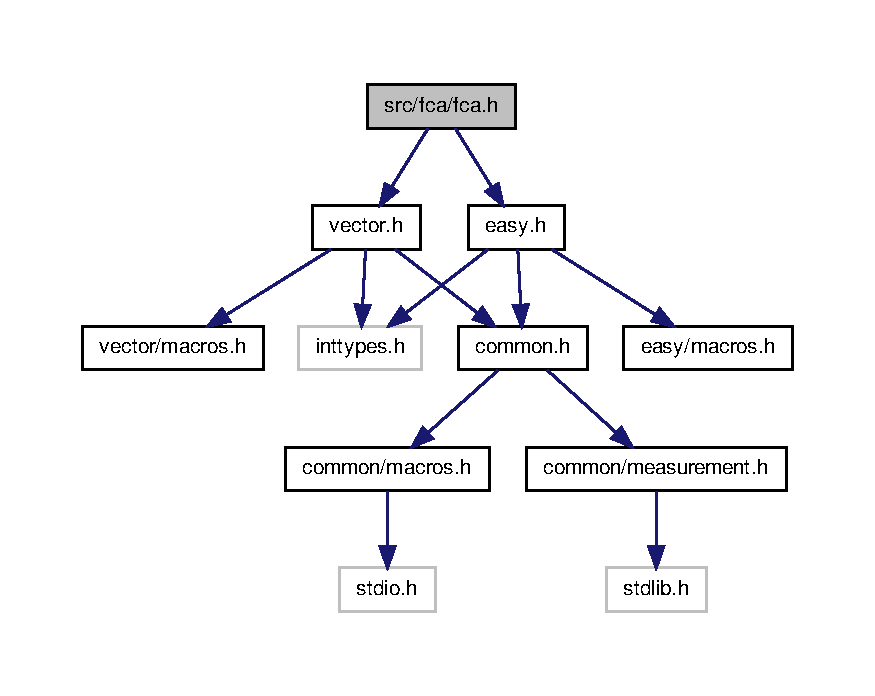
\includegraphics[width=350pt]{fca_8h__incl}
\end{center}
\end{figure}
\-This graph shows which files directly or indirectly include this file\-:
\nopagebreak
\begin{figure}[H]
\begin{center}
\leavevmode
\includegraphics[width=150pt]{fca_8h__dep__incl}
\end{center}
\end{figure}


\subsection{\-Detailed \-Description}
\hyperlink{fca_8h}{fca.\-h}, (c) 2013, \-Immanuel \-Albrecht; \-Dresden \-University of \-Technology, \-Professur für die \-Psychologie des \-Lernen und \-Lehrens \-This program is free software\-: you can redistribute it and/or modify it under the terms of the \-G\-N\-U \-General \-Public \-License as published by the \-Free \-Software \-Foundation, either version 3 of the \-License, or (at your option) any later version.

\-This program is distributed in the hope that it will be useful, but \-W\-I\-T\-H\-O\-U\-T \-A\-N\-Y \-W\-A\-R\-R\-A\-N\-T\-Y; without even the implied warranty of \-M\-E\-R\-C\-H\-A\-N\-T\-A\-B\-I\-L\-I\-T\-Y or \-F\-I\-T\-N\-E\-S\-S \-F\-O\-R \-A \-P\-A\-R\-T\-I\-C\-U\-L\-A\-R \-P\-U\-R\-P\-O\-S\-E. \-See the \-G\-N\-U \-General \-Public \-License for more details.

\-You should have received a copy of the \-G\-N\-U \-General \-Public \-License along with this program. \-If not, see $<$\href{http://www.gnu.org/licenses/}{\tt http\-://www.\-gnu.\-org/licenses/}$>$.

this file contains the public interface to the formal context analysis code

this file provides both easy and vector routines 

\-Definition in file \hyperlink{fca_8h_source}{fca.\-h}.


\hypertarget{vector_8h}{\section{src/fca/vector.h \-File \-Reference}
\label{vector_8h}\index{src/fca/vector.\-h@{src/fca/vector.\-h}}
}


\hyperlink{vector_8h}{vector.\-h}, (c) 2013, \-Immanuel \-Albrecht; \-Dresden \-University of \-Technology, \-Professur für die \-Psychologie des \-Lernen und \-Lehrens  


{\ttfamily \#include $<$inttypes.\-h$>$}\*
{\ttfamily \#include \char`\"{}common.\-h\char`\"{}}\*
{\ttfamily \#include \char`\"{}vector/macros.\-h\char`\"{}}\*
{\ttfamily \#include \char`\"{}vector/measurement.\-h\char`\"{}}\*
\-Include dependency graph for vector.\-h\-:\nopagebreak
\begin{figure}[H]
\begin{center}
\leavevmode
\includegraphics[width=350pt]{vector_8h__incl}
\end{center}
\end{figure}
\-This graph shows which files directly or indirectly include this file\-:\nopagebreak
\begin{figure}[H]
\begin{center}
\leavevmode
\includegraphics[width=350pt]{vector_8h__dep__incl}
\end{center}
\end{figure}
\subsection*{\-Data \-Structures}
\begin{DoxyCompactItemize}
\item 
struct \hyperlink{structsFormalIntentV}{s\-Formal\-Intent\-V}
\begin{DoxyCompactList}\small\item\em intent structure of a formal concept \end{DoxyCompactList}\end{DoxyCompactItemize}
\subsection*{\-Typedefs}
\begin{DoxyCompactItemize}
\item 
typedef uint64\-\_\-t $\ast$ \hyperlink{vector_8h_aae617489ac88fff15979050721fe581f}{\-Incidence\-Vector}
\begin{DoxyCompactList}\small\item\em type of compressed attribute vectors \end{DoxyCompactList}\item 
typedef struct s\-Formal\-Context\-V $\ast$ \hyperlink{vector_8h_a98aafc7ce3efff805e9add08680b731f}{\-Formal\-Context\-V}
\item 
typedef struct \hyperlink{structsFormalIntentV}{s\-Formal\-Intent\-V} \hyperlink{vector_8h_ac16f78f4584c2341c43ac5c0c3a758c8}{\-Formal\-Intent\-V}
\begin{DoxyCompactList}\small\item\em intent structure of a formal concept \end{DoxyCompactList}\end{DoxyCompactItemize}
\subsection*{\-Functions}
\begin{DoxyCompactItemize}
\item 
\hyperlink{vector_8h_a98aafc7ce3efff805e9add08680b731f}{\-Formal\-Context\-V} \hyperlink{vector_8h_aa4f8b6d04c1fb2dd35fa8324bd383913}{new\-Formal\-Context\-V} (unsigned int objects, unsigned int attributes)
\begin{DoxyCompactList}\small\item\em create a new formal context \end{DoxyCompactList}\item 
void \hyperlink{vector_8h_a42ae183692b566f6d12c9db27e8f7ec1}{delete\-Formal\-Context\-V} (\hyperlink{vector_8h_a98aafc7ce3efff805e9add08680b731f}{\-Formal\-Context\-V} $\ast$ctx)
\begin{DoxyCompactList}\small\item\em deletes the formal context $\ast$ctx, and sets the pointer to zero \end{DoxyCompactList}\item 
void \hyperlink{vector_8h_aa4861d8f750bb9786aa32c55a683764b}{write\-Formal\-Context\-V} (\hyperlink{vector_8h_a98aafc7ce3efff805e9add08680b731f}{\-Formal\-Context\-V} ctx, const char $\ast$filename)
\begin{DoxyCompactList}\small\item\em save the context ctx at the given file location \end{DoxyCompactList}\item 
\hyperlink{vector_8h_a98aafc7ce3efff805e9add08680b731f}{\-Formal\-Context\-V} \hyperlink{vector_8h_a9b6b69f5062c68c30c5e1e6d56ea37bc}{new\-Formal\-Context\-From\-File\-V} (const char $\ast$filename)
\begin{DoxyCompactList}\small\item\em create a new formal context object from a .cxt file \end{DoxyCompactList}\end{DoxyCompactItemize}


\subsection{\-Detailed \-Description}
\hyperlink{vector_8h}{vector.\-h}, (c) 2013, \-Immanuel \-Albrecht; \-Dresden \-University of \-Technology, \-Professur für die \-Psychologie des \-Lernen und \-Lehrens \-This program is free software\-: you can redistribute it and/or modify it under the terms of the \-G\-N\-U \-General \-Public \-License as published by the \-Free \-Software \-Foundation, either version 3 of the \-License, or (at your option) any later version.

\-This program is distributed in the hope that it will be useful, but \-W\-I\-T\-H\-O\-U\-T \-A\-N\-Y \-W\-A\-R\-R\-A\-N\-T\-Y; without even the implied warranty of \-M\-E\-R\-C\-H\-A\-N\-T\-A\-B\-I\-L\-I\-T\-Y or \-F\-I\-T\-N\-E\-S\-S \-F\-O\-R \-A \-P\-A\-R\-T\-I\-C\-U\-L\-A\-R \-P\-U\-R\-P\-O\-S\-E. \-See the \-G\-N\-U \-General \-Public \-License for more details.

\-You should have received a copy of the \-G\-N\-U \-General \-Public \-License along with this program. \-If not, see $<$\href{http://www.gnu.org/licenses/}{\tt http\-://www.\-gnu.\-org/licenses/}$>$.

\-This header file provides interfaces with the faster \-Incidence\-Vector implementations 

\-Definition in file \hyperlink{vector_8h_source}{vector.\-h}.



\subsection{\-Typedef \-Documentation}
\hypertarget{vector_8h_a98aafc7ce3efff805e9add08680b731f}{\index{vector.\-h@{vector.\-h}!\-Formal\-Context\-V@{\-Formal\-Context\-V}}
\index{\-Formal\-Context\-V@{\-Formal\-Context\-V}!vector.h@{vector.\-h}}
\subsubsection[{\-Formal\-Context\-V}]{\setlength{\rightskip}{0pt plus 5cm}typedef struct s\-Formal\-Context\-V$\ast$ {\bf \-Formal\-Context\-V}}}\label{vector_8h_a98aafc7ce3efff805e9add08680b731f}


\-Definition at line 44 of file vector.\-h.

\hypertarget{vector_8h_ac16f78f4584c2341c43ac5c0c3a758c8}{\index{vector.\-h@{vector.\-h}!\-Formal\-Intent\-V@{\-Formal\-Intent\-V}}
\index{\-Formal\-Intent\-V@{\-Formal\-Intent\-V}!vector.h@{vector.\-h}}
\subsubsection[{\-Formal\-Intent\-V}]{\setlength{\rightskip}{0pt plus 5cm}typedef struct {\bf s\-Formal\-Intent\-V}  {\bf \-Formal\-Intent\-V}}}\label{vector_8h_ac16f78f4584c2341c43ac5c0c3a758c8}


intent structure of a formal concept 

\hypertarget{vector_8h_aae617489ac88fff15979050721fe581f}{\index{vector.\-h@{vector.\-h}!\-Incidence\-Vector@{\-Incidence\-Vector}}
\index{\-Incidence\-Vector@{\-Incidence\-Vector}!vector.h@{vector.\-h}}
\subsubsection[{\-Incidence\-Vector}]{\setlength{\rightskip}{0pt plus 5cm}typedef uint64\-\_\-t$\ast$ {\bf \-Incidence\-Vector}}}\label{vector_8h_aae617489ac88fff15979050721fe581f}


type of compressed attribute vectors 



\-Definition at line 36 of file vector.\-h.



\subsection{\-Function \-Documentation}
\hypertarget{vector_8h_a42ae183692b566f6d12c9db27e8f7ec1}{\index{vector.\-h@{vector.\-h}!delete\-Formal\-Context\-V@{delete\-Formal\-Context\-V}}
\index{delete\-Formal\-Context\-V@{delete\-Formal\-Context\-V}!vector.h@{vector.\-h}}
\subsubsection[{delete\-Formal\-Context\-V}]{\setlength{\rightskip}{0pt plus 5cm}void {\bf delete\-Formal\-Context\-V} (
\begin{DoxyParamCaption}
\item[{{\bf \-Formal\-Context\-V} $\ast$}]{ctx}
\end{DoxyParamCaption}
)}}\label{vector_8h_a42ae183692b566f6d12c9db27e8f7ec1}


deletes the formal context $\ast$ctx, and sets the pointer to zero 


\begin{DoxyParams}{\-Parameters}
{\em ctx} & pointer to the formal context object to be deleted \\
\hline
\end{DoxyParams}


\-Definition at line 82 of file fca\-V.\-c.



\-References smy\-Formal\-Context\-V\-::attribute\-Names, smy\-Formal\-Context\-V\-::attributes, smy\-Formal\-Context\-V\-::incidence, smy\-Formal\-Context\-V\-::object\-Names, smy\-Formal\-Context\-V\-::objects, and \-R\-E\-T\-U\-R\-N\-\_\-\-I\-F\-\_\-\-Z\-E\-R\-O.


\begin{DoxyCode}
{
    RETURN_IF_ZERO(ctx);
    RETURN_IF_ZERO(*ctx);

    myFormalContextV *c;

    c = (myFormalContextV*) *ctx;

    *ctx = 0;

    for (unsigned int var = 0; var < c->attributes; ++var)
    {
        free(c->attributeNames[var]);
    }

    for (unsigned int var = 0; var < c->objects; ++var)
    {
        free(c->objectNames[var]);
    }

    free(c->objectNames);
    free(c->attributeNames);
    free(c->incidence);
    free(c);
}
\end{DoxyCode}
\hypertarget{vector_8h_a9b6b69f5062c68c30c5e1e6d56ea37bc}{\index{vector.\-h@{vector.\-h}!new\-Formal\-Context\-From\-File\-V@{new\-Formal\-Context\-From\-File\-V}}
\index{new\-Formal\-Context\-From\-File\-V@{new\-Formal\-Context\-From\-File\-V}!vector.h@{vector.\-h}}
\subsubsection[{new\-Formal\-Context\-From\-File\-V}]{\setlength{\rightskip}{0pt plus 5cm}{\bf \-Formal\-Context\-V} {\bf new\-Formal\-Context\-From\-File\-V} (
\begin{DoxyParamCaption}
\item[{const char $\ast$}]{filename}
\end{DoxyParamCaption}
)}}\label{vector_8h_a9b6b69f5062c68c30c5e1e6d56ea37bc}


create a new formal context object from a .cxt file 


\begin{DoxyParams}{\-Parameters}
{\em filename} & \\
\hline
\end{DoxyParams}
\begin{DoxyReturn}{\-Returns}
the formal context that has been read from the given file 
\end{DoxyReturn}
this should never happen, right?

we read all data

free memory and return

\-Definition at line 116 of file fca\-V.\-c.



\-References smy\-Formal\-Context\-V\-::attribute\-Names, \-C\-R\-O\-S\-S\-V, \-I\-N\-P\-U\-T\-B\-U\-F\-F\-E\-R\-S\-I\-Z\-E, \-M\-I\-N, new\-Formal\-Context\-V(), smy\-Formal\-Context\-V\-::object\-Names, \-R\-E\-T\-U\-R\-N\-\_\-\-Z\-E\-R\-O\-\_\-\-I\-F\-\_\-\-Z\-E\-R\-O, and \-R\-O\-W.


\begin{DoxyCode}
{
    char *line;
    size_t len;

    len = (INPUTBUFFERSIZE);
    line = malloc(sizeof(char) * len);

    FILE *file;

    if (strcmp(filename, "-") == 0)
    {
        file = stdin;
    }
    else
    {
        file = fopen(filename, "r");
        RETURN_ZERO_IF_ZERO(file);
    }

    ssize_t read;

    unsigned int line_nbr;
    line_nbr = 0;

    unsigned int objects;
    unsigned int attributes;

    attributes = 0;
    objects = 0;

    myFormalContextV *ctx;
    ctx = 0;

    while ((read = getline(&line, &len, file)) != -1)
    {

        if (read == 0)
            break;
        line[read - 1] = 0;

        if (line_nbr == 0)
        {
            if (strcmp(line, "B"))
            {
                fprintf(stderr, "File '%s' is not a .cxt file\n", filename);
                goto grace;
            }
        }
        else if (line_nbr == 1)
        {
            //empty line
        }
        else if (line_nbr == 2)
        {
#pragma GCC diagnostic push
#pragma GCC diagnostic ignored "-Wsign-conversion"
            objects = atoi(line);
#pragma GCC diagnostic pop
        }
        else if (line_nbr == 3)
        {
#pragma GCC diagnostic push
#pragma GCC diagnostic ignored "-Wsign-conversion"
            attributes = atoi(line);
            ctx = (myFormalContextV *) newFormalContextV(objects, attributes);
#pragma GCC diagnostic pop
        }
        else if (line_nbr == 4)
        {
            //empty line
        }
        else if (line_nbr < objects + 5)
        {

            unsigned int i;
            i = line_nbr - 5;

            free(ctx->objectNames[i]);
            ctx->objectNames[i] = strdup(line);

        }
        else if (line_nbr < objects + attributes + 5)
        {
            unsigned int i;
            i = line_nbr - 5 - objects;

            free(ctx->attributeNames[i]);
            ctx->attributeNames[i] = strdup(line);
        }
        else if (line_nbr < objects * 2 + attributes + 5)
        {
            unsigned int i;
            i = line_nbr - 5 - objects - attributes;

            unsigned int width;
            width = MIN((unsigned int)strlen(line),attributes);

            for (unsigned int var = 0; var < width; ++var)
            {
                if ((line[var] == 'x') || (line[var] == 'X')
                        || (line[var] == '1'))
                {
                    CROSSV(ROW(i, ctx), var);
                }
            }

        }
        else
        {
            break;
        }

        line_nbr++;
    }

    grace: if (file != stdin)
    {
        fclose(file);
    }

    free(line);

    return (FormalContextV) ctx;
}
\end{DoxyCode}


\-Here is the call graph for this function\-:\nopagebreak
\begin{figure}[H]
\begin{center}
\leavevmode
\includegraphics[width=350pt]{vector_8h_a9b6b69f5062c68c30c5e1e6d56ea37bc_cgraph}
\end{center}
\end{figure}


\hypertarget{vector_8h_aa4f8b6d04c1fb2dd35fa8324bd383913}{\index{vector.\-h@{vector.\-h}!new\-Formal\-Context\-V@{new\-Formal\-Context\-V}}
\index{new\-Formal\-Context\-V@{new\-Formal\-Context\-V}!vector.h@{vector.\-h}}
\subsubsection[{new\-Formal\-Context\-V}]{\setlength{\rightskip}{0pt plus 5cm}{\bf \-Formal\-Context\-V} {\bf new\-Formal\-Context\-V} (
\begin{DoxyParamCaption}
\item[{unsigned int}]{objects, }
\item[{unsigned int}]{attributes}
\end{DoxyParamCaption}
)}}\label{vector_8h_aa4f8b6d04c1fb2dd35fa8324bd383913}


create a new formal context 


\begin{DoxyParams}{\-Parameters}
{\em objects} & object count \\
\hline
{\em attributes} & attribute count \\
\hline
\end{DoxyParams}
\begin{DoxyReturn}{\-Returns}
a new \-Formal\-Context object 
\end{DoxyReturn}


\-Definition at line 40 of file fca\-V.\-c.



\-References smy\-Formal\-Context\-V\-::attribute\-Names, smy\-Formal\-Context\-V\-::attributes, smy\-Formal\-Context\-V\-::incidence, smy\-Formal\-Context\-V\-::object\-Names, smy\-Formal\-Context\-V\-::objects, \-W\-I\-D\-T\-H, and smy\-Formal\-Context\-V\-::width.



\-Referenced by new\-Formal\-Context\-From\-File\-V().


\begin{DoxyCode}
{
    myFormalContextV *ctx = malloc(sizeof(myFormalContextV));

    ctx->attributes = attributes;
    ctx->objects = objects;
    ctx->width = WIDTH(attributes);

#pragma GCC diagnostic push
#pragma GCC diagnostic ignored "-Wsign-conversion"

    ctx->attributeNames = calloc(attributes, sizeof(char*));
    ctx->objectNames = calloc(objects, sizeof(char*));

#pragma GCC diagnostic pop

    for (unsigned int var = 0; var < attributes; ++var)
    {
        ctx->attributeNames[var] = calloc(1, sizeof(char));
    }

    for (unsigned int var = 0; var < objects; ++var)
    {
        ctx->objectNames[var] = calloc(1, sizeof(char));
    }

#pragma GCC diagnostic push
#pragma GCC diagnostic ignored "-Wsign-conversion"

    ctx->incidence = calloc(objects * ctx->width, sizeof(uint64_t));

#pragma GCC diagnostic pop

    return (FormalContextV) ctx;
}
\end{DoxyCode}
\hypertarget{vector_8h_aa4861d8f750bb9786aa32c55a683764b}{\index{vector.\-h@{vector.\-h}!write\-Formal\-Context\-V@{write\-Formal\-Context\-V}}
\index{write\-Formal\-Context\-V@{write\-Formal\-Context\-V}!vector.h@{vector.\-h}}
\subsubsection[{write\-Formal\-Context\-V}]{\setlength{\rightskip}{0pt plus 5cm}void {\bf write\-Formal\-Context\-V} (
\begin{DoxyParamCaption}
\item[{{\bf \-Formal\-Context\-V}}]{ctx, }
\item[{const char $\ast$}]{filename}
\end{DoxyParamCaption}
)}}\label{vector_8h_aa4861d8f750bb9786aa32c55a683764b}


save the context ctx at the given file location 


\begin{DoxyParams}{\-Parameters}
{\em ctx} & \\
\hline
{\em filename} & \\
\hline
\end{DoxyParams}


\-Definition at line 258 of file fca\-V.\-c.



\-References smy\-Formal\-Context\-V\-::attribute\-Names, smy\-Formal\-Context\-V\-::attributes, \-I\-N\-C\-I\-D\-E\-S\-V, smy\-Formal\-Context\-V\-::object\-Names, smy\-Formal\-Context\-V\-::objects, \-R\-E\-T\-U\-R\-N\-\_\-\-I\-F\-\_\-\-Z\-E\-R\-O, and \-R\-O\-W.


\begin{DoxyCode}
{
    RETURN_IF_ZERO(ctx);
    RETURN_IF_ZERO(filename);

    FILE* file;
    file = fopen(filename, "w");

    RETURN_IF_ZERO(file);

    myFormalContextV *c;
    c = (myFormalContextV*) ctx;

    fprintf(file, "B\n\n%zu\n%zu\n\n", c->objects, c->attributes);

    for (unsigned int var = 0; var < c->objects; ++var)
    {
        fputs(c->objectNames[var], file);
        fputs("\n", file);
    }

    for (unsigned int var = 0; var < c->attributes; ++var)
    {
        fputs(c->attributeNames[var], file);
        fputs("\n", file);
    }

    for (unsigned int g = 0; g < c->objects; ++g)
    {
        for (unsigned int m = 0; m < c->attributes; ++m)
        {
            if ( INCIDESV(ROW(g, c), m))
                fputs("X", file);
            else
                fputs(".", file);
        }
        fputs("\n", file);
    }

    fclose(file);
}
\end{DoxyCode}

\hypertarget{fcaV_8c}{\section{src/vector/fca\-V.c \-File \-Reference}
\label{fcaV_8c}\index{src/vector/fca\-V.\-c@{src/vector/fca\-V.\-c}}
}


\hyperlink{fcaV_8c}{fca\-V.\-c}, (c) 2013, \-Immanuel \-Albrecht; \-Dresden \-University of \-Technology, \-Professur für die \-Psychologie des \-Lernen und \-Lehrens  


{\ttfamily \#include $<$stdio.\-h$>$}\*
{\ttfamily \#include $<$stdlib.\-h$>$}\*
{\ttfamily \#include $<$string.\-h$>$}\*
{\ttfamily \#include \char`\"{}../fca.\-h\char`\"{}}\*
{\ttfamily \#include \char`\"{}../fca\-\_\-macros.\-h\char`\"{}}\*
{\ttfamily \#include \char`\"{}macros.\-h\char`\"{}}\*
{\ttfamily \#include \char`\"{}structs.\-h\char`\"{}}\*
{\ttfamily \#include \char`\"{}private.\-h\char`\"{}}\*
\-Include dependency graph for fca\-V.\-c\-:
\nopagebreak
\begin{figure}[H]
\begin{center}
\leavevmode
\includegraphics[width=350pt]{fcaV_8c__incl}
\end{center}
\end{figure}
\subsection*{\-Functions}
\begin{DoxyCompactItemize}
\item 
\hyperlink{fca_8h_a98aafc7ce3efff805e9add08680b731f}{\-Formal\-Context\-V} \hyperlink{fcaV_8c_aa4f8b6d04c1fb2dd35fa8324bd383913}{new\-Formal\-Context\-V} (unsigned int objects, unsigned int attributes)
\begin{DoxyCompactList}\small\item\em create a new formal context \end{DoxyCompactList}\item 
void \hyperlink{fcaV_8c_a42ae183692b566f6d12c9db27e8f7ec1}{delete\-Formal\-Context\-V} (\hyperlink{fca_8h_a98aafc7ce3efff805e9add08680b731f}{\-Formal\-Context\-V} $\ast$ctx)
\begin{DoxyCompactList}\small\item\em deletes the formal context $\ast$ctx, and sets the pointer to zero \end{DoxyCompactList}\item 
\hyperlink{fca_8h_a98aafc7ce3efff805e9add08680b731f}{\-Formal\-Context\-V} \hyperlink{fcaV_8c_a9b6b69f5062c68c30c5e1e6d56ea37bc}{new\-Formal\-Context\-From\-File\-V} (const char $\ast$filename)
\begin{DoxyCompactList}\small\item\em create a new formal context object from a .cxt file \end{DoxyCompactList}\item 
void \hyperlink{fcaV_8c_aa4861d8f750bb9786aa32c55a683764b}{write\-Formal\-Context\-V} (\hyperlink{fca_8h_a98aafc7ce3efff805e9add08680b731f}{\-Formal\-Context\-V} ctx, const char $\ast$filename)
\begin{DoxyCompactList}\small\item\em save the context ctx at the given file location \end{DoxyCompactList}\item 
int \hyperlink{fcaV_8c_ae9e90e93ffaf10b9da1a3e3f789d00e9}{count\-Context\-Concepts\-V} (\hyperlink{fca_8h_a98aafc7ce3efff805e9add08680b731f}{\-Formal\-Context\-V} ctx)
\begin{DoxyCompactList}\small\item\em counts the concepts in the concept lattice of ctx, using next closure algorithm \end{DoxyCompactList}\item 
void \hyperlink{fcaV_8c_adcfe1beba7f75ea7a6e4230916b6a65a}{close\-Intent\-V} (\hyperlink{fca_8h_a98aafc7ce3efff805e9add08680b731f}{\-Formal\-Context\-V} ctx, const \hyperlink{fca_8h_aae617489ac88fff15979050721fe581f}{\-Incidence\-Vector} input, \hyperlink{fca_8h_aae617489ac88fff15979050721fe581f}{\-Incidence\-Vector} output)
\begin{DoxyCompactList}\small\item\em close an attribute set, i.\-e. \end{DoxyCompactList}\item 
int \hyperlink{fcaV_8c_a55d40e1b5169e4466d00cb930c67e0ef}{intent\-Cmp\-V} (size\-\_\-t attributes, const \hyperlink{fca_8h_aae617489ac88fff15979050721fe581f}{\-Incidence\-Vector} minus, const \hyperlink{fca_8h_aae617489ac88fff15979050721fe581f}{\-Incidence\-Vector} plus)
\begin{DoxyCompactList}\small\item\em compare two intent vectors \end{DoxyCompactList}\item 
\hyperlink{vector_2structs_8h_abe3c190ec3375121cbfe3afff517b9b9}{my\-Formal\-Concept\-Intent\-Chunk\-V} $\ast$ \hyperlink{fcaV_8c_ab5c9a71c810ad1eeeb5f8ff78d77d899}{new\-Concept\-Chunk\-V} (size\-\_\-t attributes)
\begin{DoxyCompactList}\small\item\em create a new formal concept chunk \end{DoxyCompactList}\item 
void \hyperlink{fcaV_8c_afd9305761d657be7c21fb81e82d72a42}{delete\-Concept\-Chunk\-V} (\hyperlink{vector_2structs_8h_abe3c190ec3375121cbfe3afff517b9b9}{my\-Formal\-Concept\-Intent\-Chunk\-V} $\ast$$\ast$c)
\begin{DoxyCompactList}\small\item\em deletes a concept chunk object and sets its pointer to zero \end{DoxyCompactList}\item 
\hyperlink{vector_2structs_8h_a6306c91d1e7b5237618bab6172a784a1}{\-Formal\-Concept\-Intent\-Bulk\-List\-V} \hyperlink{fcaV_8c_abda612c4305c29a37b6501e18d94ebc5}{new\-Concept\-Bulk\-V} (size\-\_\-t attributes)
\begin{DoxyCompactList}\small\item\em creates a new formal concept intent bulk list \end{DoxyCompactList}\item 
\hyperlink{vector_2structs_8h_a6306c91d1e7b5237618bab6172a784a1}{\-Formal\-Concept\-Intent\-Bulk\-List\-V} \hyperlink{fcaV_8c_a90151fdf1b3ef3201deb2e1ab752729d}{new\-Concept\-Bulk\-From\-Context\-V} (\hyperlink{fca_8h_a98aafc7ce3efff805e9add08680b731f}{\-Formal\-Context\-V} ctx)
\begin{DoxyCompactList}\small\item\em creates a new formal concept intent chunk and fills it with the intents of all formal concepts in the concept lattice of ctx, using next closure algorithm \end{DoxyCompactList}\item 
void \hyperlink{fcaV_8c_ac1443261c57cc1d3db9361c188cd9c96}{write\-Concepts\-To\-File\-V} (\hyperlink{fca_8h_a98aafc7ce3efff805e9add08680b731f}{\-Formal\-Context\-V} ctx, \hyperlink{vector_2structs_8h_a6306c91d1e7b5237618bab6172a784a1}{\-Formal\-Concept\-Intent\-Bulk\-List\-V} root, const char $\ast$filename)
\begin{DoxyCompactList}\small\item\em write a list of concept intents into a .cxt file \end{DoxyCompactList}\item 
void \hyperlink{fcaV_8c_aa2cf22779998982c65e3762c7e2c2c84}{delete\-Concept\-Bulk\-V} (\hyperlink{vector_2structs_8h_a6306c91d1e7b5237618bab6172a784a1}{\-Formal\-Concept\-Intent\-Bulk\-List\-V} $\ast$root\-Node)
\begin{DoxyCompactList}\small\item\em deletes the entire bulk list \end{DoxyCompactList}\item 
size\-\_\-t \hyperlink{fcaV_8c_a7d53642e5953e35c86ef0425858d707e}{count\-Concepts\-In\-Bulk\-V} (\hyperlink{vector_2structs_8h_a6306c91d1e7b5237618bab6172a784a1}{\-Formal\-Concept\-Intent\-Bulk\-List\-V} root)
\begin{DoxyCompactList}\small\item\em use this for bulks that are filled in order \end{DoxyCompactList}\item 
\hyperlink{vector_2structs_8h_a6306c91d1e7b5237618bab6172a784a1}{\-Formal\-Concept\-Intent\-Bulk\-List\-V} \hyperlink{fcaV_8c_aa6cc62f8dfd08ef795a932cd06e69b91}{add\-Concept\-To\-Bulk\-V} (\hyperlink{vector_2structs_8h_a6306c91d1e7b5237618bab6172a784a1}{\-Formal\-Concept\-Intent\-Bulk\-List\-V} root, const \hyperlink{fca_8h_aae617489ac88fff15979050721fe581f}{\-Incidence\-Vector} intent)
\begin{DoxyCompactList}\small\item\em copies the given intent to the bulk denoted by the root node. \end{DoxyCompactList}\end{DoxyCompactItemize}


\subsection{\-Detailed \-Description}
\hyperlink{fcaV_8c}{fca\-V.\-c}, (c) 2013, \-Immanuel \-Albrecht; \-Dresden \-University of \-Technology, \-Professur für die \-Psychologie des \-Lernen und \-Lehrens \-This program is free software\-: you can redistribute it and/or modify it under the terms of the \-G\-N\-U \-General \-Public \-License as published by the \-Free \-Software \-Foundation, either version 3 of the \-License, or (at your option) any later version.

\-This program is distributed in the hope that it will be useful, but \-W\-I\-T\-H\-O\-U\-T \-A\-N\-Y \-W\-A\-R\-R\-A\-N\-T\-Y; without even the implied warranty of \-M\-E\-R\-C\-H\-A\-N\-T\-A\-B\-I\-L\-I\-T\-Y or \-F\-I\-T\-N\-E\-S\-S \-F\-O\-R \-A \-P\-A\-R\-T\-I\-C\-U\-L\-A\-R \-P\-U\-R\-P\-O\-S\-E. \-See the \-G\-N\-U \-General \-Public \-License for more details.

\-You should have received a copy of the \-G\-N\-U \-General \-Public \-License along with this program. \-If not, see $<$\href{http://www.gnu.org/licenses/}{\tt http\-://www.\-gnu.\-org/licenses/}$>$. this file contains general formal context related operations and routines with \-Incidence\-Vector implementation 

\-Definition in file \hyperlink{fcaV_8c_source}{fca\-V.\-c}.



\subsection{\-Function \-Documentation}
\hypertarget{fcaV_8c_aa6cc62f8dfd08ef795a932cd06e69b91}{\index{fca\-V.\-c@{fca\-V.\-c}!add\-Concept\-To\-Bulk\-V@{add\-Concept\-To\-Bulk\-V}}
\index{add\-Concept\-To\-Bulk\-V@{add\-Concept\-To\-Bulk\-V}!fcaV.c@{fca\-V.\-c}}
\subsubsection[{add\-Concept\-To\-Bulk\-V}]{\setlength{\rightskip}{0pt plus 5cm}{\bf \-Formal\-Concept\-Intent\-Bulk\-List\-V} {\bf add\-Concept\-To\-Bulk\-V} (
\begin{DoxyParamCaption}
\item[{{\bf \-Formal\-Concept\-Intent\-Bulk\-List\-V}}]{root, }
\item[{const {\bf \-Incidence\-Vector}}]{intent}
\end{DoxyParamCaption}
)}}\label{fcaV_8c_aa6cc62f8dfd08ef795a932cd06e69b91}


copies the given intent to the bulk denoted by the root node. 


\begin{DoxyParams}{\-Parameters}
{\em root} & root node of the bulk \\
\hline
{\em intent} & read-\/only pointer to an array of \-Incidence\-Cell\mbox{[}root-\/$>$attributes\mbox{]}\\
\hline
\end{DoxyParams}
\begin{DoxyReturn}{\-Returns}
the node where the intent was added to the last chunk 
\end{DoxyReturn}


\-Definition at line 837 of file fca\-V.\-c.



\-References s\-Formal\-Concept\-Intent\-Bulk\-Node\-V\-::attributes, \-B\-U\-L\-K\-S\-I\-Z\-E\-V, s\-Formal\-Concept\-Intent\-Bulk\-Node\-V\-::chunks, \-C\-H\-U\-N\-K\-S\-I\-Z\-E\-V, new\-Concept\-Bulk\-V(), new\-Concept\-Chunk\-V(), s\-Formal\-Concept\-Intent\-Bulk\-Node\-V\-::next, \-R\-E\-T\-U\-R\-N\-\_\-\-Z\-E\-R\-O\-\_\-\-I\-F\-\_\-\-Z\-E\-R\-O, \-R\-O\-W, smy\-Formal\-Concept\-Intent\-Chunk\-V\-::size, s\-Formal\-Concept\-Intent\-Bulk\-Node\-V\-::size, and s\-Formal\-Concept\-Intent\-Bulk\-Node\-V\-::width.



\-Referenced by new\-Concept\-Bulk\-From\-Context\-V(), and next\-Closure\-V\-X1().


\begin{DoxyCode}
{
    RETURN_ZERO_IF_ZERO(root);


    do
    {

        if (root->size == 0)
        {
            root->chunks[0] = newConceptChunkV(root->attributes);
            root->size = 1;
        }

        size_t last_index;
        last_index = root->size - 1;

        if (root->chunks[last_index]->size == CHUNKSIZEV)
        {
            if (root->size == BULKSIZEV)
            {
                if (root->next == 0)
                {
                    root->next = newConceptBulkV(root->attributes);
                }
                root = root->next;
                continue;
            }
            else
            {
                last_index = root->size++;
                root->chunks[last_index] = newConceptChunkV(root->attributes);
            }
        }

#pragma GCC diagnostic push
#pragma GCC diagnostic ignored "-Wsign-conversion"

        memcpy( ROW(root->chunks[last_index]->size, root->chunks[last_index]),
                intent, sizeof(uint64_t) * root->width);

#pragma GCC diagnostic pop

        root->chunks[last_index]->size++;

        break;

    } while (1);

    return root;
}
\end{DoxyCode}


\-Here is the call graph for this function\-:
\nopagebreak
\begin{figure}[H]
\begin{center}
\leavevmode
\includegraphics[width=332pt]{fcaV_8c_aa6cc62f8dfd08ef795a932cd06e69b91_cgraph}
\end{center}
\end{figure}


\hypertarget{fcaV_8c_adcfe1beba7f75ea7a6e4230916b6a65a}{\index{fca\-V.\-c@{fca\-V.\-c}!close\-Intent\-V@{close\-Intent\-V}}
\index{close\-Intent\-V@{close\-Intent\-V}!fcaV.c@{fca\-V.\-c}}
\subsubsection[{close\-Intent\-V}]{\setlength{\rightskip}{0pt plus 5cm}void {\bf close\-Intent\-V} (
\begin{DoxyParamCaption}
\item[{{\bf \-Formal\-Context\-V}}]{ctx, }
\item[{const {\bf \-Incidence\-Vector}}]{input, }
\item[{{\bf \-Incidence\-Vector}}]{output}
\end{DoxyParamCaption}
)}}\label{fcaV_8c_adcfe1beba7f75ea7a6e4230916b6a65a}


close an attribute set, i.\-e. 

\hyperlink{vector_2private_8h}{vector/private.\-h}, (c) 2013, \-Immanuel \-Albrecht; \-Dresden \-University of \-Technology, \-Professur für die \-Psychologie des \-Lernen und \-Lehrens

add further attributes


\begin{DoxyParams}{\-Parameters}
{\em ctx} & formal context \\
\hline
{\em input} & the intent set that is to be closed \\
\hline
{\em output} & the closure intent'' wrt. ctx \\
\hline
\end{DoxyParams}
some attribute is not present for this object -\/$>$ next object

remove attributes that are not common among all objects that have the input attributes

\-Definition at line 413 of file fca\-V.\-c.



\-References smy\-Formal\-Context\-V\-::attributes, \-M\-A\-S\-K\-V\-E\-C\-T\-O\-R, smy\-Formal\-Context\-V\-::objects, \-R\-O\-W, and smy\-Formal\-Context\-V\-::width.



\-Referenced by count\-Context\-Concepts\-V(), new\-Concept\-Bulk\-From\-Context\-V(), and next\-Closure\-V\-X1().


\begin{DoxyCode}
{

    myFormalContextV* I;
    I = (myFormalContextV*) ctx;
    for (size_t var = 0; var < I->width; ++var)
    {
        output[var] = ~0ULL;
    }

    MASKVECTOR(output, I->attributes);

    for (size_t g = 0; g < I->objects; ++g)
    {
        int good;
        good = 1;

        for (size_t i = 0; i < I->width; ++i)
        {
            if ((input[i]) & (~(ROW(g,I)[i])))
            {
                good = 0;
                break;
            }

        }

        if (good)
        {
            for (size_t i = 0; i < I->width; ++i)
            {
                output[i] &= ROW(g,I)[i];
            }
        }
    }
}
\end{DoxyCode}
\hypertarget{fcaV_8c_a7d53642e5953e35c86ef0425858d707e}{\index{fca\-V.\-c@{fca\-V.\-c}!count\-Concepts\-In\-Bulk\-V@{count\-Concepts\-In\-Bulk\-V}}
\index{count\-Concepts\-In\-Bulk\-V@{count\-Concepts\-In\-Bulk\-V}!fcaV.c@{fca\-V.\-c}}
\subsubsection[{count\-Concepts\-In\-Bulk\-V}]{\setlength{\rightskip}{0pt plus 5cm}size\-\_\-t {\bf count\-Concepts\-In\-Bulk\-V} (
\begin{DoxyParamCaption}
\item[{{\bf \-Formal\-Concept\-Intent\-Bulk\-List\-V}}]{root}
\end{DoxyParamCaption}
)}}\label{fcaV_8c_a7d53642e5953e35c86ef0425858d707e}


use this for bulks that are filled in order 


\begin{DoxyParams}{\-Parameters}
{\em root} & \\
\hline
\end{DoxyParams}
\begin{DoxyReturn}{\-Returns}
number of concepts in bulk 
\end{DoxyReturn}
count the full chunks

and the last chunk

\-Definition at line 802 of file fca\-V.\-c.



\-References s\-Formal\-Concept\-Intent\-Bulk\-Node\-V\-::chunks, \-C\-H\-U\-N\-K\-S\-I\-Z\-E\-V, s\-Formal\-Concept\-Intent\-Bulk\-Node\-V\-::next, \-R\-E\-T\-U\-R\-N\-\_\-\-Z\-E\-R\-O\-\_\-\-I\-F\-\_\-\-Z\-E\-R\-O, smy\-Formal\-Concept\-Intent\-Chunk\-V\-::size, and s\-Formal\-Concept\-Intent\-Bulk\-Node\-V\-::size.



\-Referenced by main(), and write\-Concepts\-To\-File\-V().


\begin{DoxyCode}
{
    RETURN_ZERO_IF_ZERO(root);

    size_t count = 0;

    while (root != 0)
    {
        if (root->size > 0)
        {
            count += CHUNKSIZEV * (root->size - 1);
            count += root->chunks[root->size - 1]->size;
        }
        root = root->next;
    }

    return count;
}
\end{DoxyCode}
\hypertarget{fcaV_8c_ae9e90e93ffaf10b9da1a3e3f789d00e9}{\index{fca\-V.\-c@{fca\-V.\-c}!count\-Context\-Concepts\-V@{count\-Context\-Concepts\-V}}
\index{count\-Context\-Concepts\-V@{count\-Context\-Concepts\-V}!fcaV.c@{fca\-V.\-c}}
\subsubsection[{count\-Context\-Concepts\-V}]{\setlength{\rightskip}{0pt plus 5cm}int {\bf count\-Context\-Concepts\-V} (
\begin{DoxyParamCaption}
\item[{{\bf \-Formal\-Context\-V}}]{ctx}
\end{DoxyParamCaption}
)}}\label{fcaV_8c_ae9e90e93ffaf10b9da1a3e3f789d00e9}


counts the concepts in the concept lattice of ctx, using next closure algorithm 


\begin{DoxyParams}{\-Parameters}
{\em ctx} & formal context \\
\hline
\end{DoxyParams}
\begin{DoxyReturn}{\-Returns}
number of concepts in context 
\end{DoxyReturn}
calculate the bottom intent of the concept lattice, i.\-e. \{\}''

begin of next\-Closure function iteration

we found the next intent

continue with \-Y for \-M

do the next\-Closure

free up memory

\-Definition at line 310 of file fca\-V.\-c.



\-References smy\-Formal\-Context\-V\-::attributes, \-C\-L\-E\-A\-R\-V, close\-Intent\-V(), \-C\-R\-I\-M\-P\-V\-A\-L\-U\-E, \-C\-R\-O\-S\-S\-V, \-I\-N\-C\-I\-D\-E\-S\-V, \-O\-F\-F\-S\-E\-T, \-R\-E\-T\-U\-R\-N\-\_\-\-Z\-E\-R\-O\-\_\-\-I\-F\-\_\-\-Z\-E\-R\-O, and smy\-Formal\-Context\-V\-::width.


\begin{DoxyCode}
{
    RETURN_ZERO_IF_ZERO(ctx);

    myFormalContextV *c;
    c = (myFormalContextV*) ctx;

    IncidenceVector M;
    IncidenceVector Y;

#pragma GCC diagnostic push
#pragma GCC diagnostic ignored "-Wsign-conversion"

    Y = calloc(c->width, sizeof(uint64_t));
    M = malloc(c->width * sizeof(uint64_t));

#pragma GCC diagnostic pop

    closeIntentV(ctx, Y, M);

    int count;

    count = 1;

    nextClosure:

    for (size_t i = c->attributes; i > 0;)
    {
        --i;

        if (!INCIDESV(M,i))
        {
            CROSSV(M, i);
            closeIntentV(ctx, M, Y);

            int good;
            good = 1;

            for (unsigned int j = 0; j < OFFSET(i); ++j)
            {
                if (Y[j] & (~(M[j])))
                {
                    good = 0;
                    break;
                }
            }
            if (good)
            {
                if (Y[OFFSET(i)] & (~M[OFFSET(i)]) & CRIMPVALUE(i))
                {
                    good = 0;
                }
            }

            if (good)
            {
                count++;

                IncidenceVector DELTA;
                DELTA = M;
                M = Y;
                Y = DELTA;
                goto nextClosure;
            }
        }

        CLEARV(M, i);
    }

    free(M);
    free(Y);

    return count;
}
\end{DoxyCode}


\-Here is the call graph for this function\-:
\nopagebreak
\begin{figure}[H]
\begin{center}
\leavevmode
\includegraphics[width=312pt]{fcaV_8c_ae9e90e93ffaf10b9da1a3e3f789d00e9_cgraph}
\end{center}
\end{figure}


\hypertarget{fcaV_8c_aa2cf22779998982c65e3762c7e2c2c84}{\index{fca\-V.\-c@{fca\-V.\-c}!delete\-Concept\-Bulk\-V@{delete\-Concept\-Bulk\-V}}
\index{delete\-Concept\-Bulk\-V@{delete\-Concept\-Bulk\-V}!fcaV.c@{fca\-V.\-c}}
\subsubsection[{delete\-Concept\-Bulk\-V}]{\setlength{\rightskip}{0pt plus 5cm}void {\bf delete\-Concept\-Bulk\-V} (
\begin{DoxyParamCaption}
\item[{{\bf \-Formal\-Concept\-Intent\-Bulk\-List\-V} $\ast$}]{root\-Node}
\end{DoxyParamCaption}
)}}\label{fcaV_8c_aa2cf22779998982c65e3762c7e2c2c84}


deletes the entire bulk list 


\begin{DoxyParams}{\-Parameters}
{\em root\-Node} & pointer to the first node \\
\hline
\end{DoxyParams}


\-Definition at line 770 of file fca\-V.\-c.



\-References s\-Formal\-Concept\-Intent\-Bulk\-Node\-V\-::chunks, delete\-Concept\-Chunk\-V(), s\-Formal\-Concept\-Intent\-Bulk\-Node\-V\-::next, \-R\-E\-T\-U\-R\-N\-\_\-\-I\-F\-\_\-\-Z\-E\-R\-O, and s\-Formal\-Concept\-Intent\-Bulk\-Node\-V\-::size.



\-Referenced by main().


\begin{DoxyCode}
{
    RETURN_IF_ZERO(rootNode);
    RETURN_IF_ZERO(*rootNode);

    FormalConceptIntentBulkListV l;
    l = *rootNode;
    *rootNode = 0;

    do
    {
        for (size_t var = 0; var < l->size; ++var)
        {
            deleteConceptChunkV(&(l->chunks[var]));
        }

        FormalConceptIntentBulkListV next;
        next = l->next;

        free(l->chunks);
        free(l);

        l = next;
    } while (l != 0);
}
\end{DoxyCode}


\-Here is the call graph for this function\-:
\nopagebreak
\begin{figure}[H]
\begin{center}
\leavevmode
\includegraphics[width=338pt]{fcaV_8c_aa2cf22779998982c65e3762c7e2c2c84_cgraph}
\end{center}
\end{figure}


\hypertarget{fcaV_8c_afd9305761d657be7c21fb81e82d72a42}{\index{fca\-V.\-c@{fca\-V.\-c}!delete\-Concept\-Chunk\-V@{delete\-Concept\-Chunk\-V}}
\index{delete\-Concept\-Chunk\-V@{delete\-Concept\-Chunk\-V}!fcaV.c@{fca\-V.\-c}}
\subsubsection[{delete\-Concept\-Chunk\-V}]{\setlength{\rightskip}{0pt plus 5cm}void {\bf delete\-Concept\-Chunk\-V} (
\begin{DoxyParamCaption}
\item[{{\bf my\-Formal\-Concept\-Intent\-Chunk\-V} $\ast$$\ast$}]{c}
\end{DoxyParamCaption}
)}}\label{fcaV_8c_afd9305761d657be7c21fb81e82d72a42}


deletes a concept chunk object and sets its pointer to zero 


\begin{DoxyParams}{\-Parameters}
{\em c} & pointer to the concept chunk to be deleted \\
\hline
\end{DoxyParams}


\-Definition at line 539 of file fca\-V.\-c.



\-References \-R\-E\-T\-U\-R\-N\-\_\-\-I\-F\-\_\-\-Z\-E\-R\-O.



\-Referenced by delete\-Concept\-Bulk\-V().


\begin{DoxyCode}
{
    RETURN_IF_ZERO(c);
    RETURN_IF_ZERO(*c);

    free((*c)->incidence);

    free(*c);
    *c = 0;
}
\end{DoxyCode}
\hypertarget{fcaV_8c_a42ae183692b566f6d12c9db27e8f7ec1}{\index{fca\-V.\-c@{fca\-V.\-c}!delete\-Formal\-Context\-V@{delete\-Formal\-Context\-V}}
\index{delete\-Formal\-Context\-V@{delete\-Formal\-Context\-V}!fcaV.c@{fca\-V.\-c}}
\subsubsection[{delete\-Formal\-Context\-V}]{\setlength{\rightskip}{0pt plus 5cm}void {\bf delete\-Formal\-Context\-V} (
\begin{DoxyParamCaption}
\item[{{\bf \-Formal\-Context\-V} $\ast$}]{ctx}
\end{DoxyParamCaption}
)}}\label{fcaV_8c_a42ae183692b566f6d12c9db27e8f7ec1}


deletes the formal context $\ast$ctx, and sets the pointer to zero 


\begin{DoxyParams}{\-Parameters}
{\em ctx} & pointer to the formal context object to be deleted \\
\hline
\end{DoxyParams}


\-Definition at line 86 of file fca\-V.\-c.



\-References smy\-Formal\-Context\-V\-::attribute\-Names, smy\-Formal\-Context\-V\-::attributes, smy\-Formal\-Context\-V\-::incidence, smy\-Formal\-Context\-V\-::object\-Names, smy\-Formal\-Context\-V\-::objects, and \-R\-E\-T\-U\-R\-N\-\_\-\-I\-F\-\_\-\-Z\-E\-R\-O.



\-Referenced by main().


\begin{DoxyCode}
{
    RETURN_IF_ZERO(ctx);
    RETURN_IF_ZERO(*ctx);

    myFormalContextV *c;

    c = (myFormalContextV*) *ctx;

    *ctx = 0;

    for (unsigned int var = 0; var < c->attributes; ++var)
    {
        free(c->attributeNames[var]);
    }

    for (unsigned int var = 0; var < c->objects; ++var)
    {
        free(c->objectNames[var]);
    }

    free(c->objectNames);
    free(c->attributeNames);
    free(c->incidence);
    free(c);
}
\end{DoxyCode}
\hypertarget{fcaV_8c_a55d40e1b5169e4466d00cb930c67e0ef}{\index{fca\-V.\-c@{fca\-V.\-c}!intent\-Cmp\-V@{intent\-Cmp\-V}}
\index{intent\-Cmp\-V@{intent\-Cmp\-V}!fcaV.c@{fca\-V.\-c}}
\subsubsection[{intent\-Cmp\-V}]{\setlength{\rightskip}{0pt plus 5cm}int {\bf intent\-Cmp\-V} (
\begin{DoxyParamCaption}
\item[{size\-\_\-t}]{attributes, }
\item[{const {\bf \-Incidence\-Vector}}]{minus, }
\item[{const {\bf \-Incidence\-Vector}}]{plus}
\end{DoxyParamCaption}
)}}\label{fcaV_8c_a55d40e1b5169e4466d00cb930c67e0ef}


compare two intent vectors 


\begin{DoxyParams}{\-Parameters}
{\em attributes} & attribute count \\
\hline
{\em minus} & \char`\"{}left\char`\"{} operand \\
\hline
{\em plus} & \char`\"{}right\char`\"{} operand \\
\hline
\end{DoxyParams}
\begin{DoxyReturn}{\-Returns}
-\/1 if minus is bigger, 1 if plus is bigger, 0 if minus and plus is the same 
\end{DoxyReturn}
in this case, \hyperlink{vector_2macros_8h_ad12dce0a7bf9d908b172a28155b3d261}{\-O\-F\-F\-S\-E\-T(attributes)} == \-O\-F\-F\-S\-E\-T(attributes-\/1)

we only check the lower bits 0 through (attributes-\/1)

\-E\-L\-S\-E\-: attributes has 64 as factor, so we have done all necessary comparisons in the first loop.

\-Definition at line 468 of file fca\-V.\-c.



\-References \-B\-I\-T\-N\-B\-R, \-C\-R\-I\-M\-P\-V\-A\-L\-U\-E, and \-O\-F\-F\-S\-E\-T.



\-Referenced by next\-Closure\-V\-X1().


\begin{DoxyCode}
{
    for (size_t var = 0; var < OFFSET(attributes); ++var)
    {
        if (minus[var] > plus[var])
            return -1;
        if (plus[var] > minus[var])
            return 1;
    }

    if (BITNBR(attributes))
    {
        uint64_t l, r;

        l = minus[OFFSET(attributes)] & CRIMPVALUE(attributes-1);
        r = plus[OFFSET(attributes)] & CRIMPVALUE(attributes-1);

        if (l > r)
            return -1;

        if (r > l)
            return 1;
    }
    return 0;
}
\end{DoxyCode}
\hypertarget{fcaV_8c_a90151fdf1b3ef3201deb2e1ab752729d}{\index{fca\-V.\-c@{fca\-V.\-c}!new\-Concept\-Bulk\-From\-Context\-V@{new\-Concept\-Bulk\-From\-Context\-V}}
\index{new\-Concept\-Bulk\-From\-Context\-V@{new\-Concept\-Bulk\-From\-Context\-V}!fcaV.c@{fca\-V.\-c}}
\subsubsection[{new\-Concept\-Bulk\-From\-Context\-V}]{\setlength{\rightskip}{0pt plus 5cm}{\bf \-Formal\-Concept\-Intent\-Bulk\-List\-V} {\bf new\-Concept\-Bulk\-From\-Context\-V} (
\begin{DoxyParamCaption}
\item[{{\bf \-Formal\-Context\-V}}]{ctx}
\end{DoxyParamCaption}
)}}\label{fcaV_8c_a90151fdf1b3ef3201deb2e1ab752729d}


creates a new formal concept intent chunk and fills it with the intents of all formal concepts in the concept lattice of ctx, using next closure algorithm 


\begin{DoxyParams}{\-Parameters}
{\em ctx} & formal context \\
\hline
\end{DoxyParams}
\begin{DoxyReturn}{\-Returns}
concept intents 
\end{DoxyReturn}
calculate the bottom intent of the concept lattice, i.\-e. \{\}''

add the bottom element of the concept lattice (a concept lattice is never empty)

begin of next\-Closure function iteration

we found the next intent

continue with \-Y for \-M

do the next\-Closure

free up memory

\-Definition at line 578 of file fca\-V.\-c.



\-References add\-Concept\-To\-Bulk\-V(), smy\-Formal\-Context\-V\-::attributes, \-C\-L\-E\-A\-R\-V, close\-Intent\-V(), \-C\-R\-I\-M\-P\-V\-A\-L\-U\-E, \-C\-R\-O\-S\-S\-V, \-I\-N\-C\-I\-D\-E\-S\-V, new\-Concept\-Bulk\-V(), \-O\-F\-F\-S\-E\-T, \-R\-E\-T\-U\-R\-N\-\_\-\-Z\-E\-R\-O\-\_\-\-I\-F\-\_\-\-Z\-E\-R\-O, and smy\-Formal\-Context\-V\-::width.



\-Referenced by main().


\begin{DoxyCode}
{
    RETURN_ZERO_IF_ZERO(ctx);

    myFormalContextV *c;
    c = (myFormalContextV*) ctx;

    IncidenceVector M;
    IncidenceVector Y;

#pragma GCC diagnostic push
#pragma GCC diagnostic ignored "-Wsign-conversion"

    Y = calloc(c->width, sizeof(uint64_t));
    M = malloc(c->width * sizeof(uint64_t));

#pragma GCC diagnostic pop

    closeIntentV(ctx, Y, M);

    FormalConceptIntentBulkListV root;
    FormalConceptIntentBulkListV last;



    root = newConceptBulkV(c->attributes);


    last = addConceptToBulkV(root, M);


    nextClosure:

    for (size_t i = c->attributes; i > 0;)
    {
        --i;

        if (!INCIDESV(M,i))
        {
            CROSSV(M, i);
            closeIntentV(ctx, M, Y);

            int good;
            good = 1;

            for (unsigned int j = 0; j < OFFSET(i); ++j)
            {
                if (Y[j] & (~(M[j])))
                {
                    good = 0;
                    break;
                }
            }
            if (good)
            {
                if (Y[OFFSET(i)] & (~M[OFFSET(i)]) & CRIMPVALUE(i))
                {
                    good = 0;
                }
            }

            if (good)
            {

                last = addConceptToBulkV(last, Y);

                IncidenceVector DELTA;
                DELTA = M;
                M = Y;
                Y = DELTA;
                goto nextClosure;
            }
        }

        CLEARV(M, i);
    }

    free(M);
    free(Y);

    return root;
}
\end{DoxyCode}


\-Here is the call graph for this function\-:
\nopagebreak
\begin{figure}[H]
\begin{center}
\leavevmode
\includegraphics[width=350pt]{fcaV_8c_a90151fdf1b3ef3201deb2e1ab752729d_cgraph}
\end{center}
\end{figure}


\hypertarget{fcaV_8c_abda612c4305c29a37b6501e18d94ebc5}{\index{fca\-V.\-c@{fca\-V.\-c}!new\-Concept\-Bulk\-V@{new\-Concept\-Bulk\-V}}
\index{new\-Concept\-Bulk\-V@{new\-Concept\-Bulk\-V}!fcaV.c@{fca\-V.\-c}}
\subsubsection[{new\-Concept\-Bulk\-V}]{\setlength{\rightskip}{0pt plus 5cm}{\bf \-Formal\-Concept\-Intent\-Bulk\-List\-V} {\bf new\-Concept\-Bulk\-V} (
\begin{DoxyParamCaption}
\item[{size\-\_\-t}]{attributes}
\end{DoxyParamCaption}
)}}\label{fcaV_8c_abda612c4305c29a37b6501e18d94ebc5}


creates a new formal concept intent bulk list 


\begin{DoxyParams}{\-Parameters}
{\em attributes} & number of attributes of the concept intents \\
\hline
\end{DoxyParams}
\begin{DoxyReturn}{\-Returns}
new formal concept intent bulk list's first node 
\end{DoxyReturn}


\-Definition at line 557 of file fca\-V.\-c.



\-References s\-Formal\-Concept\-Intent\-Bulk\-Node\-V\-::attributes, \-B\-U\-L\-K\-S\-I\-Z\-E\-V, s\-Formal\-Concept\-Intent\-Bulk\-Node\-V\-::chunks, s\-Formal\-Concept\-Intent\-Bulk\-Node\-V\-::next, s\-Formal\-Concept\-Intent\-Bulk\-Node\-V\-::size, \-W\-I\-D\-T\-H, and s\-Formal\-Concept\-Intent\-Bulk\-Node\-V\-::width.



\-Referenced by add\-Concept\-To\-Bulk\-V(), new\-Concept\-Bulk\-From\-Context\-V(), and next\-Closure\-V\-X1().


\begin{DoxyCode}
{
    FormalConceptIntentBulkListV l;
    l = malloc(sizeof(struct sFormalConceptIntentBulkNodeV));

    l->attributes = attributes;
    l->width = WIDTH(attributes);
    l->size = 0;
    l->chunks = calloc(BULKSIZEV, sizeof(myFormalConceptIntentChunkV*));
    l->next = 0;
    return l;
}
\end{DoxyCode}
\hypertarget{fcaV_8c_ab5c9a71c810ad1eeeb5f8ff78d77d899}{\index{fca\-V.\-c@{fca\-V.\-c}!new\-Concept\-Chunk\-V@{new\-Concept\-Chunk\-V}}
\index{new\-Concept\-Chunk\-V@{new\-Concept\-Chunk\-V}!fcaV.c@{fca\-V.\-c}}
\subsubsection[{new\-Concept\-Chunk\-V}]{\setlength{\rightskip}{0pt plus 5cm}{\bf my\-Formal\-Concept\-Intent\-Chunk\-V}$\ast$ {\bf new\-Concept\-Chunk\-V} (
\begin{DoxyParamCaption}
\item[{size\-\_\-t}]{attributes}
\end{DoxyParamCaption}
)}}\label{fcaV_8c_ab5c9a71c810ad1eeeb5f8ff78d77d899}


create a new formal concept chunk 


\begin{DoxyParams}{\-Parameters}
{\em attributes} & number of attributes of the hosting formal context \\
\hline
\end{DoxyParams}
\begin{DoxyReturn}{\-Returns}
a new concept chunk object 
\end{DoxyReturn}


\-Definition at line 511 of file fca\-V.\-c.



\-References smy\-Formal\-Concept\-Intent\-Chunk\-V\-::attributes, \-C\-H\-U\-N\-K\-S\-I\-Z\-E\-V, smy\-Formal\-Concept\-Intent\-Chunk\-V\-::incidence, smy\-Formal\-Concept\-Intent\-Chunk\-V\-::size, \-W\-I\-D\-T\-H, and smy\-Formal\-Concept\-Intent\-Chunk\-V\-::width.



\-Referenced by add\-Concept\-To\-Bulk\-V().


\begin{DoxyCode}
{

    myFormalConceptIntentChunkV *c;

    c = malloc(sizeof(myFormalConceptIntentChunkV));

    c->attributes = attributes;
    c->width = WIDTH(attributes);
    c->size = 0;


#pragma GCC diagnostic push
#pragma GCC diagnostic ignored "-Wsign-conversion"

    c->incidence = calloc(c->width * CHUNKSIZEV, sizeof(uint64_t));

#pragma GCC diagnostic pop

    return c;
}
\end{DoxyCode}
\hypertarget{fcaV_8c_a9b6b69f5062c68c30c5e1e6d56ea37bc}{\index{fca\-V.\-c@{fca\-V.\-c}!new\-Formal\-Context\-From\-File\-V@{new\-Formal\-Context\-From\-File\-V}}
\index{new\-Formal\-Context\-From\-File\-V@{new\-Formal\-Context\-From\-File\-V}!fcaV.c@{fca\-V.\-c}}
\subsubsection[{new\-Formal\-Context\-From\-File\-V}]{\setlength{\rightskip}{0pt plus 5cm}{\bf \-Formal\-Context\-V} {\bf new\-Formal\-Context\-From\-File\-V} (
\begin{DoxyParamCaption}
\item[{const char $\ast$}]{filename}
\end{DoxyParamCaption}
)}}\label{fcaV_8c_a9b6b69f5062c68c30c5e1e6d56ea37bc}


create a new formal context object from a .cxt file 


\begin{DoxyParams}{\-Parameters}
{\em filename} & \\
\hline
\end{DoxyParams}
\begin{DoxyReturn}{\-Returns}
the formal context that has been read from the given file 
\end{DoxyReturn}
this should never happen, right?

we read all data

free memory and return

\-Definition at line 120 of file fca\-V.\-c.



\-References smy\-Formal\-Context\-V\-::attribute\-Names, \-C\-R\-O\-S\-S\-V, \-I\-N\-P\-U\-T\-B\-U\-F\-F\-E\-R\-S\-I\-Z\-E, \-M\-I\-N, new\-Formal\-Context\-V(), smy\-Formal\-Context\-V\-::object\-Names, \-R\-E\-T\-U\-R\-N\-\_\-\-Z\-E\-R\-O\-\_\-\-I\-F\-\_\-\-Z\-E\-R\-O, and \-R\-O\-W.



\-Referenced by main().


\begin{DoxyCode}
{
    char *line;
    size_t len;

    len = (INPUTBUFFERSIZE);
    line = malloc(sizeof(char) * len);

    FILE *file;

    if (strcmp(filename, "-") == 0)
    {
        file = stdin;
    }
    else
    {
        file = fopen(filename, "r");
        RETURN_ZERO_IF_ZERO(file);
    }

    ssize_t read;

    unsigned int line_nbr;
    line_nbr = 0;

    unsigned int objects;
    unsigned int attributes;

    attributes = 0;
    objects = 0;

    myFormalContextV *ctx;
    ctx = 0;

    while ((read = getline(&line, &len, file)) != -1)
    {

        if (read == 0)
            break;
        line[read - 1] = 0;

        if (line_nbr == 0)
        {
            if (strcmp(line, "B"))
            {
                fprintf(stderr, "File '%s' is not a .cxt file\n", filename);
                goto grace;
            }
        }
        else if (line_nbr == 1)
        {
            //empty line
        }
        else if (line_nbr == 2)
        {
#pragma GCC diagnostic push
#pragma GCC diagnostic ignored "-Wsign-conversion"
            objects = atoi(line);
#pragma GCC diagnostic pop
        }
        else if (line_nbr == 3)
        {
#pragma GCC diagnostic push
#pragma GCC diagnostic ignored "-Wsign-conversion"
            attributes = atoi(line);
            ctx = (myFormalContextV *) newFormalContextV(objects, attributes);
#pragma GCC diagnostic pop
        }
        else if (line_nbr == 4)
        {
            //empty line
        }
        else if (line_nbr < objects + 5)
        {

            unsigned int i;
            i = line_nbr - 5;

            free(ctx->objectNames[i]);
            ctx->objectNames[i] = strdup(line);

        }
        else if (line_nbr < objects + attributes + 5)
        {
            unsigned int i;
            i = line_nbr - 5 - objects;

            free(ctx->attributeNames[i]);
            ctx->attributeNames[i] = strdup(line);
        }
        else if (line_nbr < objects * 2 + attributes + 5)
        {
            unsigned int i;
            i = line_nbr - 5 - objects - attributes;

            unsigned int width;
            width = MIN((unsigned int)strlen(line),attributes);

            for (unsigned int var = 0; var < width; ++var)
            {
                if ((line[var] == 'x') || (line[var] == 'X')
                        || (line[var] == '1'))
                {
                    CROSSV(ROW(i, ctx), var);
                }
            }

        }
        else
        {
            break;
        }

        line_nbr++;
    }

    grace: if (file != stdin)
    {
        fclose(file);
    }

    free(line);

    return (FormalContextV) ctx;
}
\end{DoxyCode}


\-Here is the call graph for this function\-:\nopagebreak
\begin{figure}[H]
\begin{center}
\leavevmode
\includegraphics[width=350pt]{fcaV_8c_a9b6b69f5062c68c30c5e1e6d56ea37bc_cgraph}
\end{center}
\end{figure}


\hypertarget{fcaV_8c_aa4f8b6d04c1fb2dd35fa8324bd383913}{\index{fca\-V.\-c@{fca\-V.\-c}!new\-Formal\-Context\-V@{new\-Formal\-Context\-V}}
\index{new\-Formal\-Context\-V@{new\-Formal\-Context\-V}!fcaV.c@{fca\-V.\-c}}
\subsubsection[{new\-Formal\-Context\-V}]{\setlength{\rightskip}{0pt plus 5cm}{\bf \-Formal\-Context\-V} {\bf new\-Formal\-Context\-V} (
\begin{DoxyParamCaption}
\item[{unsigned int}]{objects, }
\item[{unsigned int}]{attributes}
\end{DoxyParamCaption}
)}}\label{fcaV_8c_aa4f8b6d04c1fb2dd35fa8324bd383913}


create a new formal context 


\begin{DoxyParams}{\-Parameters}
{\em objects} & object count \\
\hline
{\em attributes} & attribute count \\
\hline
\end{DoxyParams}
\begin{DoxyReturn}{\-Returns}
a new \-Formal\-Context object 
\end{DoxyReturn}


\-Definition at line 44 of file fca\-V.\-c.



\-References smy\-Formal\-Context\-V\-::attribute\-Names, smy\-Formal\-Context\-V\-::attributes, smy\-Formal\-Context\-V\-::incidence, smy\-Formal\-Context\-V\-::object\-Names, smy\-Formal\-Context\-V\-::objects, \-W\-I\-D\-T\-H, and smy\-Formal\-Context\-V\-::width.



\-Referenced by new\-Formal\-Context\-From\-File\-V().


\begin{DoxyCode}
{
    myFormalContextV *ctx = malloc(sizeof(myFormalContextV));

    ctx->attributes = attributes;
    ctx->objects = objects;
    ctx->width = WIDTH(attributes);

#pragma GCC diagnostic push
#pragma GCC diagnostic ignored "-Wsign-conversion"

    ctx->attributeNames = calloc(attributes, sizeof(char*));
    ctx->objectNames = calloc(objects, sizeof(char*));

#pragma GCC diagnostic pop

    for (unsigned int var = 0; var < attributes; ++var)
    {
        ctx->attributeNames[var] = calloc(1, sizeof(char));
    }

    for (unsigned int var = 0; var < objects; ++var)
    {
        ctx->objectNames[var] = calloc(1, sizeof(char));
    }

#pragma GCC diagnostic push
#pragma GCC diagnostic ignored "-Wsign-conversion"

    ctx->incidence = calloc(objects * ctx->width, sizeof(uint64_t));

#pragma GCC diagnostic pop

    return (FormalContextV) ctx;
}
\end{DoxyCode}
\hypertarget{fcaV_8c_ac1443261c57cc1d3db9361c188cd9c96}{\index{fca\-V.\-c@{fca\-V.\-c}!write\-Concepts\-To\-File\-V@{write\-Concepts\-To\-File\-V}}
\index{write\-Concepts\-To\-File\-V@{write\-Concepts\-To\-File\-V}!fcaV.c@{fca\-V.\-c}}
\subsubsection[{write\-Concepts\-To\-File\-V}]{\setlength{\rightskip}{0pt plus 5cm}void {\bf write\-Concepts\-To\-File\-V} (
\begin{DoxyParamCaption}
\item[{{\bf \-Formal\-Context\-V}}]{ctx, }
\item[{{\bf \-Formal\-Concept\-Intent\-Bulk\-List\-V}}]{root, }
\item[{const char $\ast$}]{filename}
\end{DoxyParamCaption}
)}}\label{fcaV_8c_ac1443261c57cc1d3db9361c188cd9c96}


write a list of concept intents into a .cxt file 


\begin{DoxyParams}{\-Parameters}
{\em ctx} & formal context (or 0, is used for attribute names) \\
\hline
{\em root} & the first node of the formal concept intent bulk \\
\hline
{\em filename} & output file name (.cxt) \\
\hline
\end{DoxyParams}


\-Definition at line 693 of file fca\-V.\-c.



\-References smy\-Formal\-Context\-V\-::attribute\-Names, smy\-Formal\-Context\-V\-::attributes, s\-Formal\-Concept\-Intent\-Bulk\-Node\-V\-::attributes, s\-Formal\-Concept\-Intent\-Bulk\-Node\-V\-::chunks, count\-Concepts\-In\-Bulk\-V(), \-I\-N\-C\-I\-D\-E\-S\-V, s\-Formal\-Concept\-Intent\-Bulk\-Node\-V\-::next, \-R\-E\-T\-U\-R\-N\-\_\-\-I\-F\-\_\-\-Z\-E\-R\-O, \-R\-O\-W, smy\-Formal\-Concept\-Intent\-Chunk\-V\-::size, s\-Formal\-Concept\-Intent\-Bulk\-Node\-V\-::size, and \-W\-A\-R\-N\-\_\-\-I\-F\-\_\-\-U\-N\-E\-Q\-U\-A\-L\-\_\-\-D\-O.



\-Referenced by main().


\begin{DoxyCode}
{
    RETURN_IF_ZERO(root);

    myFormalContextV* c;

    if (ctx != 0)
    {
        c = (myFormalContextV*) ctx;

        WARN_IF_UNEQUAL_DO(c->attributes, root->attributes, c = 0);
    }
    else
    {
        c = 0;
    }

    RETURN_IF_ZERO(filename);

    FILE* file;
    file = fopen(filename, "w");

    RETURN_IF_ZERO(file);

    size_t objects;
    objects = countConceptsInBulkV(root);

    fprintf(file, "B\n\n%zu\n%zu\n\n", objects, root->attributes);

    for (size_t var = 0; var < objects; ++var)
    {
        fprintf(file, "C%8zu\n", (var + 1));
    }

    if (c != 0)
    {
        for (size_t var = 0; var < c->attributes; ++var)
        {
            fputs(c->attributeNames[var], file);
            fputs("\n", file);
        }
    }
    else
    {
        for (size_t var = 0; var < root->attributes; ++var)
        {
            fprintf(file, "m%8zu\n", (var + 1));
        }
    }

    for (; root != 0; root = root->next)
    {
        for (size_t chunk = 0; chunk < root->size; ++chunk)
        {
            for (size_t g = 0; g < root->chunks[chunk]->size; ++g)
            {
                for (size_t m = 0; m < root->attributes; ++m)
                {
                    if (INCIDESV(ROW(g, root->chunks[chunk]), m))
                        fputs("X", file);
                    else
                        fputs(".", file);
                }
                fputs("\n", file);
            }
        }
    }

    fclose(file);
}
\end{DoxyCode}


\-Here is the call graph for this function\-:
\nopagebreak
\begin{figure}[H]
\begin{center}
\leavevmode
\includegraphics[width=348pt]{fcaV_8c_ac1443261c57cc1d3db9361c188cd9c96_cgraph}
\end{center}
\end{figure}


\hypertarget{fcaV_8c_aa4861d8f750bb9786aa32c55a683764b}{\index{fca\-V.\-c@{fca\-V.\-c}!write\-Formal\-Context\-V@{write\-Formal\-Context\-V}}
\index{write\-Formal\-Context\-V@{write\-Formal\-Context\-V}!fcaV.c@{fca\-V.\-c}}
\subsubsection[{write\-Formal\-Context\-V}]{\setlength{\rightskip}{0pt plus 5cm}void {\bf write\-Formal\-Context\-V} (
\begin{DoxyParamCaption}
\item[{{\bf \-Formal\-Context\-V}}]{ctx, }
\item[{const char $\ast$}]{filename}
\end{DoxyParamCaption}
)}}\label{fcaV_8c_aa4861d8f750bb9786aa32c55a683764b}


save the context ctx at the given file location 


\begin{DoxyParams}{\-Parameters}
{\em ctx} & \\
\hline
{\em filename} & \\
\hline
\end{DoxyParams}


\-Definition at line 262 of file fca\-V.\-c.



\-References smy\-Formal\-Context\-V\-::attribute\-Names, smy\-Formal\-Context\-V\-::attributes, \-I\-N\-C\-I\-D\-E\-S\-V, smy\-Formal\-Context\-V\-::object\-Names, smy\-Formal\-Context\-V\-::objects, \-R\-E\-T\-U\-R\-N\-\_\-\-I\-F\-\_\-\-Z\-E\-R\-O, and \-R\-O\-W.



\-Referenced by main().


\begin{DoxyCode}
{
    RETURN_IF_ZERO(ctx);
    RETURN_IF_ZERO(filename);

    FILE* file;
    file = fopen(filename, "w");

    RETURN_IF_ZERO(file);

    myFormalContextV *c;
    c = (myFormalContextV*) ctx;

    fprintf(file, "B\n\n%zu\n%zu\n\n", c->objects, c->attributes);

    for (unsigned int var = 0; var < c->objects; ++var)
    {
        fputs(c->objectNames[var], file);
        fputs("\n", file);
    }

    for (unsigned int var = 0; var < c->attributes; ++var)
    {
        fputs(c->attributeNames[var], file);
        fputs("\n", file);
    }

    for (unsigned int g = 0; g < c->objects; ++g)
    {
        for (unsigned int m = 0; m < c->attributes; ++m)
        {
            if ( INCIDESV(ROW(g, c), m))
                fputs("X", file);
            else
                fputs(".", file);
        }
        fputs("\n", file);
    }

    fclose(file);
}
\end{DoxyCode}

\hypertarget{fcaVnextClosureX_8c}{\section{src/vector/fca\-Vnext\-Closure\-X.c \-File \-Reference}
\label{fcaVnextClosureX_8c}\index{src/vector/fca\-Vnext\-Closure\-X.\-c@{src/vector/fca\-Vnext\-Closure\-X.\-c}}
}


this file contains a multi-\/threading next\-Closure implementation using the \-Incidence\-Vector implementation  


{\ttfamily \#include $<$stdio.\-h$>$}\*
{\ttfamily \#include $<$stdlib.\-h$>$}\*
{\ttfamily \#include $<$string.\-h$>$}\*
{\ttfamily \#include $<$pthread.\-h$>$}\*
{\ttfamily \#include \char`\"{}../fca.\-h\char`\"{}}\*
{\ttfamily \#include \char`\"{}../fca\-\_\-macros.\-h\char`\"{}}\*
{\ttfamily \#include \char`\"{}macros.\-h\char`\"{}}\*
{\ttfamily \#include \char`\"{}structs.\-h\char`\"{}}\*
{\ttfamily \#include \char`\"{}private.\-h\char`\"{}}\*
\-Include dependency graph for fca\-Vnext\-Closure\-X.\-c\-:
\nopagebreak
\begin{figure}[H]
\begin{center}
\leavevmode
\includegraphics[width=350pt]{fcaVnextClosureX_8c__incl}
\end{center}
\end{figure}
\subsection*{\-Data \-Structures}
\begin{DoxyCompactItemize}
\item 
struct \hyperlink{structsnextClosureVX1Params}{snext\-Closure\-V\-X1\-Params}
\end{DoxyCompactItemize}
\subsection*{\-Defines}
\begin{DoxyCompactItemize}
\item 
\#define \hyperlink{fcaVnextClosureX_8c_a68c72a16f9628758cc5a8d2210ccd674}{intent\-Cmp}~!!\-E\-R\-R\-O\-R!!
\begin{DoxyCompactList}\small\item\em \hyperlink{fcaVnextClosureX_8c}{fca\-Vnext\-Closure\-X.\-c}, (c) 2013, \-Immanuel \-Albrecht; \-Dresden \-University of \-Technology, \-Professur für die \-Psychologie des \-Lernen und \-Lehrens \end{DoxyCompactList}\end{DoxyCompactItemize}
\subsection*{\-Typedefs}
\begin{DoxyCompactItemize}
\item 
typedef struct \*
\hyperlink{structsnextClosureVX1Params}{snext\-Closure\-V\-X1\-Params} $\ast$ \hyperlink{fcaVnextClosureX_8c_a642c21f1fdfe45b4801b52956461901d}{next\-Closure\-V\-X1\-Params}
\end{DoxyCompactItemize}
\subsection*{\-Functions}
\begin{DoxyCompactItemize}
\item 
\hyperlink{vector_2structs_8h_a6306c91d1e7b5237618bab6172a784a1}{\-Formal\-Concept\-Intent\-Bulk\-List\-V} \hyperlink{fcaVnextClosureX_8c_adcbb382ceada973214f6bbeca05cb279}{next\-Closure\-V\-X1} (\hyperlink{fca_8h_a98aafc7ce3efff805e9add08680b731f}{\-Formal\-Context\-V} ctx, const \hyperlink{fca_8h_aae617489ac88fff15979050721fe581f}{\-Incidence\-Vector} start, const \hyperlink{fca_8h_aae617489ac88fff15979050721fe581f}{\-Incidence\-Vector} stop)
\begin{DoxyCompactList}\small\item\em creates a new formal concept intent chunk and fills it with the intents of all formal concepts in the concept lattice of ctx, using next closure algorithm, that are in a given lexicographic interval of the powerset \end{DoxyCompactList}\item 
void $\ast$ \hyperlink{fcaVnextClosureX_8c_a93c37a01d282f3ab4d5ee7ff52028140}{call\-Next\-Closure\-V\-X1} (void $\ast$params)
\item 
\hyperlink{vector_2structs_8h_a6306c91d1e7b5237618bab6172a784a1}{\-Formal\-Concept\-Intent\-Bulk\-List\-V} \hyperlink{fcaVnextClosureX_8c_a858241e44987c35c2ae688f2797f2a30}{next\-Closure\-V\-X} (\hyperlink{fca_8h_a98aafc7ce3efff805e9add08680b731f}{\-Formal\-Context\-V} ctx)
\begin{DoxyCompactList}\small\item\em creates a new formal concept intent chunk and fills it with the intents of all formal concepts in the concept lattice of ctx, using a parallel next closure algorithm with up to 8 threads \end{DoxyCompactList}\end{DoxyCompactItemize}


\subsection{\-Detailed \-Description}
this file contains a multi-\/threading next\-Closure implementation using the \-Incidence\-Vector implementation 

\-Definition in file \hyperlink{fcaVnextClosureX_8c_source}{fca\-Vnext\-Closure\-X.\-c}.



\subsection{\-Define \-Documentation}
\hypertarget{fcaVnextClosureX_8c_a68c72a16f9628758cc5a8d2210ccd674}{\index{fca\-Vnext\-Closure\-X.\-c@{fca\-Vnext\-Closure\-X.\-c}!intent\-Cmp@{intent\-Cmp}}
\index{intent\-Cmp@{intent\-Cmp}!fcaVnextClosureX.c@{fca\-Vnext\-Closure\-X.\-c}}
\subsubsection[{intent\-Cmp}]{\setlength{\rightskip}{0pt plus 5cm}\#define {\bf intent\-Cmp}~!!\-E\-R\-R\-O\-R!!}}\label{fcaVnextClosureX_8c_a68c72a16f9628758cc5a8d2210ccd674}


\hyperlink{fcaVnextClosureX_8c}{fca\-Vnext\-Closure\-X.\-c}, (c) 2013, \-Immanuel \-Albrecht; \-Dresden \-University of \-Technology, \-Professur für die \-Psychologie des \-Lernen und \-Lehrens 

\-This program is free software\-: you can redistribute it and/or modify it under the terms of the \-G\-N\-U \-General \-Public \-License as published by the \-Free \-Software \-Foundation, either version 3 of the \-License, or (at your option) any later version.

\-This program is distributed in the hope that it will be useful, but \-W\-I\-T\-H\-O\-U\-T \-A\-N\-Y \-W\-A\-R\-R\-A\-N\-T\-Y; without even the implied warranty of \-M\-E\-R\-C\-H\-A\-N\-T\-A\-B\-I\-L\-I\-T\-Y or \-F\-I\-T\-N\-E\-S\-S \-F\-O\-R \-A \-P\-A\-R\-T\-I\-C\-U\-L\-A\-R \-P\-U\-R\-P\-O\-S\-E. \-See the \-G\-N\-U \-General \-Public \-License for more details.

\-You should have received a copy of the \-G\-N\-U \-General \-Public \-License along with this program. \-If not, see $<$\href{http://www.gnu.org/licenses/}{\tt http\-://www.\-gnu.\-org/licenses/}$>$. 

\-Definition at line 31 of file fca\-Vnext\-Closure\-X.\-c.



\subsection{\-Typedef \-Documentation}
\hypertarget{fcaVnextClosureX_8c_a642c21f1fdfe45b4801b52956461901d}{\index{fca\-Vnext\-Closure\-X.\-c@{fca\-Vnext\-Closure\-X.\-c}!next\-Closure\-V\-X1\-Params@{next\-Closure\-V\-X1\-Params}}
\index{next\-Closure\-V\-X1\-Params@{next\-Closure\-V\-X1\-Params}!fcaVnextClosureX.c@{fca\-Vnext\-Closure\-X.\-c}}
\subsubsection[{next\-Closure\-V\-X1\-Params}]{\setlength{\rightskip}{0pt plus 5cm}typedef struct {\bf snext\-Closure\-V\-X1\-Params}$\ast$ {\bf next\-Closure\-V\-X1\-Params}}}\label{fcaVnextClosureX_8c_a642c21f1fdfe45b4801b52956461901d}


\subsection{\-Function \-Documentation}
\hypertarget{fcaVnextClosureX_8c_a93c37a01d282f3ab4d5ee7ff52028140}{\index{fca\-Vnext\-Closure\-X.\-c@{fca\-Vnext\-Closure\-X.\-c}!call\-Next\-Closure\-V\-X1@{call\-Next\-Closure\-V\-X1}}
\index{call\-Next\-Closure\-V\-X1@{call\-Next\-Closure\-V\-X1}!fcaVnextClosureX.c@{fca\-Vnext\-Closure\-X.\-c}}
\subsubsection[{call\-Next\-Closure\-V\-X1}]{\setlength{\rightskip}{0pt plus 5cm}void$\ast$ {\bf call\-Next\-Closure\-V\-X1} (
\begin{DoxyParamCaption}
\item[{void $\ast$}]{params}
\end{DoxyParamCaption}
)}}\label{fcaVnextClosureX_8c_a93c37a01d282f3ab4d5ee7ff52028140}


\-Definition at line 184 of file fca\-Vnext\-Closure\-X.\-c.



\-References snext\-Closure\-V\-X1\-Params\-::ctx, next\-Closure\-V\-X1(), snext\-Closure\-V\-X1\-Params\-::r\-Val, snext\-Closure\-V\-X1\-Params\-::start, and snext\-Closure\-V\-X1\-Params\-::stop.



\-Referenced by next\-Closure\-V\-X().


\begin{DoxyCode}
{
    nextClosureVX1Params p;
    p = (nextClosureVX1Params) params;

    p->rVal = nextClosureVX1(p->ctx, p->start, p->stop);

    return 0;
}
\end{DoxyCode}


\-Here is the call graph for this function\-:
\nopagebreak
\begin{figure}[H]
\begin{center}
\leavevmode
\includegraphics[width=350pt]{fcaVnextClosureX_8c_a93c37a01d282f3ab4d5ee7ff52028140_cgraph}
\end{center}
\end{figure}


\hypertarget{fcaVnextClosureX_8c_a858241e44987c35c2ae688f2797f2a30}{\index{fca\-Vnext\-Closure\-X.\-c@{fca\-Vnext\-Closure\-X.\-c}!next\-Closure\-V\-X@{next\-Closure\-V\-X}}
\index{next\-Closure\-V\-X@{next\-Closure\-V\-X}!fcaVnextClosureX.c@{fca\-Vnext\-Closure\-X.\-c}}
\subsubsection[{next\-Closure\-V\-X}]{\setlength{\rightskip}{0pt plus 5cm}{\bf \-Formal\-Concept\-Intent\-Bulk\-List\-V} {\bf next\-Closure\-V\-X} (
\begin{DoxyParamCaption}
\item[{{\bf \-Formal\-Context\-V}}]{ctx}
\end{DoxyParamCaption}
)}}\label{fcaVnextClosureX_8c_a858241e44987c35c2ae688f2797f2a30}


creates a new formal concept intent chunk and fills it with the intents of all formal concepts in the concept lattice of ctx, using a parallel next closure algorithm with up to 8 threads 


\begin{DoxyParams}{\-Parameters}
{\em ctx} & formal context \\
\hline
\end{DoxyParams}
\begin{DoxyReturn}{\-Returns}
concept intents 
\end{DoxyReturn}


\-Definition at line 203 of file fca\-Vnext\-Closure\-X.\-c.



\-References smy\-Formal\-Context\-V\-::attributes, call\-Next\-Closure\-V\-X1(), \-C\-R\-O\-S\-S\-V, snext\-Closure\-V\-X1\-Params\-::ctx, s\-Formal\-Concept\-Intent\-Bulk\-Node\-V\-::next, next\-Closure\-V\-X1(), \-R\-E\-T\-U\-R\-N\-\_\-\-Z\-E\-R\-O\-\_\-\-I\-F\-\_\-\-Z\-E\-R\-O, snext\-Closure\-V\-X1\-Params\-::r\-Val, snext\-Closure\-V\-X1\-Params\-::start, snext\-Closure\-V\-X1\-Params\-::stop, and smy\-Formal\-Context\-V\-::width.



\-Referenced by main().


\begin{DoxyCode}
{
    RETURN_ZERO_IF_ZERO(ctx);

    myFormalContextV *c;
    c = (myFormalContextV*) ctx;

    size_t N;

    N = 1;

    if (c->attributes >= 3)
        N = 8;
    else if (c->attributes >= 2)
        N = 4;
    else if (c->attributes >= 1)
        N = 2;

    if (N < 2)
        return nextClosureVX1(ctx, 0, 0);

    IncidenceVector bounds;
    bounds = calloc(c->width * (N - 1), sizeof(uint64_t));

    if (N == 2)
    {
        CROSSV(bounds, 0);
    }
    else if (N == 4)
    {
        CROSSV(bounds, 1); //01

        CROSSV(bounds + c->width, 0); //10

        CROSSV(bounds + c->width * 2, 1); //11
        CROSSV(bounds + c->width * 2, 0);
    }
    else if (N == 8)
    {
        CROSSV(bounds, 2); // 001

        CROSSV(bounds + c->width, 1); //010

        CROSSV(bounds + c->width * 2, 2); //011
        CROSSV(bounds + c->width * 2, 1);

        CROSSV(bounds + c->width * 3, 0); //100

        CROSSV(bounds + c->width * 4, 0); //101
        CROSSV(bounds + c->width * 4, 2);

        CROSSV(bounds + c->width * 5, 1); //110
        CROSSV(bounds + c->width * 5, 0);

        CROSSV(bounds + c->width * 6, 0); //111
        CROSSV(bounds + c->width * 6, 1);
        CROSSV(bounds + c->width * 6, 2);
    }

//  for (int i = 0; i < N - 1; ++i)
//  {
//      printf("BOUND %16llx\n", *(bounds + i *
       c->width)&CRIMPVALUE(c->attributes-1));
//      if (i > 0)
//          printf("CMP %d\n",
//                  intentCmpV(c->attributes, bounds + (i - 1) * c->width,
//                          bounds + i * c->width));
//  }


    nextClosureVX1Params chunks;
    chunks = malloc(N * sizeof(struct snextClosureVX1Params));

    pthread_t *threads;
    threads = malloc(N * sizeof(pthread_t));

    for (size_t i = 0; i < N; ++i)
    {
        chunks[i].ctx = ctx;
        if (i > 0)
            chunks[i].start = (bounds + c->width * (i - 1));
        else
            chunks[i].start = 0;

        if (i < N - 1)
            chunks[i].stop = (bounds + c->width * (i));
        else
            chunks[i].stop = 0;
    }

    for (size_t i = 0; i < N; ++i)
    {
        pthread_create(&threads[i], 0, callNextClosureVX1, (void*) &chunks[i]);
    }

    for (size_t i = 0; i < N; ++i)
    {
        pthread_join(threads[i], 0);
    }

//  for (size_t i = 0; i < N; ++i)
//  {
//      printf("%zu thread: counts %zu\n", i,
//              countConceptsInBulkV(chunks[i].rVal));
//  }

    FormalConceptIntentBulkListV root;
    FormalConceptIntentBulkListV last;

    root = chunks[0].rVal;
    last = root;

    for (size_t var = 1; var < N; ++var)
    {

        while (last->next)
            last = last->next;

        last->next = chunks[var].rVal;
    }

    free(bounds);
    free(chunks);

    return root;
}
\end{DoxyCode}


\-Here is the call graph for this function\-:
\nopagebreak
\begin{figure}[H]
\begin{center}
\leavevmode
\includegraphics[width=350pt]{fcaVnextClosureX_8c_a858241e44987c35c2ae688f2797f2a30_cgraph}
\end{center}
\end{figure}


\hypertarget{fcaVnextClosureX_8c_adcbb382ceada973214f6bbeca05cb279}{\index{fca\-Vnext\-Closure\-X.\-c@{fca\-Vnext\-Closure\-X.\-c}!next\-Closure\-V\-X1@{next\-Closure\-V\-X1}}
\index{next\-Closure\-V\-X1@{next\-Closure\-V\-X1}!fcaVnextClosureX.c@{fca\-Vnext\-Closure\-X.\-c}}
\subsubsection[{next\-Closure\-V\-X1}]{\setlength{\rightskip}{0pt plus 5cm}{\bf \-Formal\-Concept\-Intent\-Bulk\-List\-V} {\bf next\-Closure\-V\-X1} (
\begin{DoxyParamCaption}
\item[{{\bf \-Formal\-Context\-V}}]{ctx, }
\item[{const {\bf \-Incidence\-Vector}}]{start, }
\item[{const {\bf \-Incidence\-Vector}}]{stop}
\end{DoxyParamCaption}
)}}\label{fcaVnextClosureX_8c_adcbb382ceada973214f6bbeca05cb279}


creates a new formal concept intent chunk and fills it with the intents of all formal concepts in the concept lattice of ctx, using next closure algorithm, that are in a given lexicographic interval of the powerset 


\begin{DoxyParams}{\-Parameters}
{\em ctx} & formal context \\
\hline
{\em start} & first attribute vector (not included if it is a concept intent) if this is zero, start with \-M=\{\}, in this case, we add the bottom concept in case of \-M''==\{\} \\
\hline
{\em stop} & last attribute vector, or zero to continue until the end \\
\hline
\end{DoxyParams}
\begin{DoxyReturn}{\-Returns}
concept intents between (start, stop\mbox{]} 
\end{DoxyReturn}
calculate the bottom intent of the concept lattice, i.\-e. \{\}''

add the bottom element of the concept lattice (a concept lattice is never empty)

begin of next\-Closure function iteration

check whether we are still in range

the (pseudo)intent \-Y is bigger than stop

we found the next intent

continue with \-Y for \-M

do the next\-Closure

free up memory

\-Definition at line 51 of file fca\-Vnext\-Closure\-X.\-c.



\-References add\-Concept\-To\-Bulk\-V(), smy\-Formal\-Context\-V\-::attributes, \-C\-L\-E\-A\-R\-V, close\-Intent\-V(), \-C\-R\-I\-M\-P\-V\-A\-L\-U\-E, \-C\-R\-O\-S\-S\-V, \-I\-N\-C\-I\-D\-E\-S\-V, intent\-Cmp\-V(), new\-Concept\-Bulk\-V(), \-O\-F\-F\-S\-E\-T, \-R\-E\-T\-U\-R\-N\-\_\-\-Z\-E\-R\-O\-\_\-\-I\-F\-\_\-\-Z\-E\-R\-O, and smy\-Formal\-Context\-V\-::width.



\-Referenced by call\-Next\-Closure\-V\-X1(), and next\-Closure\-V\-X().


\begin{DoxyCode}
{
    RETURN_ZERO_IF_ZERO(ctx);

    myFormalContextV *c;
    c = (myFormalContextV*) ctx;

    IncidenceVector M;
    IncidenceVector Y;

    Y = calloc(c->width, sizeof(uint64_t));
    M = malloc(c->width * sizeof(uint64_t));

    FormalConceptIntentBulkListV root;
    FormalConceptIntentBulkListV last;

    root = newConceptBulkV(c->attributes);

    if (start)
    {
        memcpy(M, start, c->width * sizeof(uint64_t));

        last = root;

    }
    else
    {

        closeIntentV(ctx, Y, M);

        last = addConceptToBulkV(root, M);
    }

    nextClosure:

    for (size_t i = c->attributes; i > 0;)
    {
        --i;

        if (!INCIDESV(M,i))
        {
            CROSSV(M, i);
            closeIntentV(ctx, M, Y);

            int good;
            good = 1;

            for (unsigned int j = 0; j < OFFSET(i); ++j)
            {
                if (Y[j] & (~(M[j])))
                {
                    good = 0;
                    break;
                }
            }
            if (good)
            {
                if (Y[OFFSET(i)] & (~M[OFFSET(i)]) & CRIMPVALUE(i))
                {
                    good = 0;
                }
            }

            if (good)
            {
                if (stop)
                {
                    if (intentCmpV(c->attributes, Y, stop) < 0)
                    {
                        goto gracefulReturn;
                    }
                }

                last = addConceptToBulkV(last, Y);

                IncidenceVector DELTA;
                DELTA = M;
                M = Y;
                Y = DELTA;
                goto nextClosure;
            }
        }

        CLEARV(M, i);
    }

    gracefulReturn:
    free(M);
    free(Y);

    return root;
}
\end{DoxyCode}


\-Here is the call graph for this function\-:
\nopagebreak
\begin{figure}[H]
\begin{center}
\leavevmode
\includegraphics[width=350pt]{fcaVnextClosureX_8c_adcbb382ceada973214f6bbeca05cb279_cgraph}
\end{center}
\end{figure}



\hypertarget{safeguard_8h}{\section{src/fca/vector/safeguard.h \-File \-Reference}
\label{safeguard_8h}\index{src/fca/vector/safeguard.\-h@{src/fca/vector/safeguard.\-h}}
}


\hyperlink{safeguard_8h}{vector/safeguard.\-h}, (c) 2013, \-Immanuel \-Albrecht; \-Dresden \-University of \-Technology, \-Professur für die \-Psychologie des \-Lernen und \-Lehrens  


\-This graph shows which files directly or indirectly include this file\-:\nopagebreak
\begin{figure}[H]
\begin{center}
\leavevmode
\includegraphics[width=350pt]{safeguard_8h__dep__incl}
\end{center}
\end{figure}
\subsection*{\-Defines}
\begin{DoxyCompactItemize}
\item 
\#define \hyperlink{safeguard_8h_a2983b695e827265a5b46ab9405446e36}{\-E\-R\-R\-O\-R\-\_\-\-T\-O\-K\-E\-N}~\-E\-A\-S\-Y\-\_\-\-V\-E\-R\-S\-I\-O\-N\-\_\-\-C\-O\-D\-E\-\_\-\-W\-I\-T\-H\-\_\-\-V\-E\-C\-T\-O\-R\-\_\-\-F\-U\-N\-C\-T\-I\-O\-N\-S
\item 
\#define \hyperlink{safeguard_8h_a239bebe1697b474e6f84945e9fb9faee}{\-C\-H\-U\-N\-K\-S\-I\-Z\-E}~\hyperlink{safeguard_8h_a2983b695e827265a5b46ab9405446e36}{\-E\-R\-R\-O\-R\-\_\-\-T\-O\-K\-E\-N}
\item 
\#define \hyperlink{safeguard_8h_a9bd2a644fe274f91e81aae543b9901c6}{\-B\-U\-L\-K\-S\-I\-Z\-E}~\hyperlink{safeguard_8h_a2983b695e827265a5b46ab9405446e36}{\-E\-R\-R\-O\-R\-\_\-\-T\-O\-K\-E\-N}
\item 
\#define \hyperlink{safeguard_8h_a7b708d6613fd52b5343713584b9fcc37}{smy\-Formal\-Context}~\hyperlink{safeguard_8h_a2983b695e827265a5b46ab9405446e36}{\-E\-R\-R\-O\-R\-\_\-\-T\-O\-K\-E\-N}
\item 
\#define \hyperlink{safeguard_8h_a5e7062722fc8c9d9f71814feb3fb65a8}{my\-Formal\-Context}~\hyperlink{safeguard_8h_a2983b695e827265a5b46ab9405446e36}{\-E\-R\-R\-O\-R\-\_\-\-T\-O\-K\-E\-N}
\item 
\#define \hyperlink{safeguard_8h_a40cc56c27bccdfdcb6fcb84969c34703}{smy\-Formal\-Concept\-Intent\-Chunk}~\hyperlink{safeguard_8h_a2983b695e827265a5b46ab9405446e36}{\-E\-R\-R\-O\-R\-\_\-\-T\-O\-K\-E\-N}
\item 
\#define \hyperlink{safeguard_8h_abfe7ce178ad72403c2d3ce8e576334c7}{my\-Formal\-Concept\-Intent\-Chunk}~\hyperlink{safeguard_8h_a2983b695e827265a5b46ab9405446e36}{\-E\-R\-R\-O\-R\-\_\-\-T\-O\-K\-E\-N}
\item 
\#define \hyperlink{safeguard_8h_ae7d463ba16fb5f6e5cc9bfc3593a5bea}{new\-Concept\-Chunk}~\hyperlink{safeguard_8h_a2983b695e827265a5b46ab9405446e36}{\-E\-R\-R\-O\-R\-\_\-\-T\-O\-K\-E\-N}
\item 
\#define \hyperlink{safeguard_8h_a091a615374256cc089c4c4ee542c1935}{delete\-Concept\-Chunk}~\hyperlink{safeguard_8h_a2983b695e827265a5b46ab9405446e36}{\-E\-R\-R\-O\-R\-\_\-\-T\-O\-K\-E\-N}
\item 
\#define \hyperlink{safeguard_8h_a50a2bfcfb537355ff2602e7552abc332}{new\-Concept\-Bulk}~\hyperlink{safeguard_8h_a2983b695e827265a5b46ab9405446e36}{\-E\-R\-R\-O\-R\-\_\-\-T\-O\-K\-E\-N}
\item 
\#define \hyperlink{safeguard_8h_a2ad12ee6d4e01ca5b4de91531fc5d8ff}{new\-Concept\-Bulk\-From\-Context}~\hyperlink{safeguard_8h_a2983b695e827265a5b46ab9405446e36}{\-E\-R\-R\-O\-R\-\_\-\-T\-O\-K\-E\-N}
\item 
\#define \hyperlink{safeguard_8h_a1038adb6a096d61bd00d22880bd3f6e7}{write\-Concepts\-To\-File}~\hyperlink{safeguard_8h_a2983b695e827265a5b46ab9405446e36}{\-E\-R\-R\-O\-R\-\_\-\-T\-O\-K\-E\-N}
\item 
\#define \hyperlink{safeguard_8h_aed8c194cd366b689a9aaf3f800e3307a}{delete\-Concept\-Bulk}~\hyperlink{safeguard_8h_a2983b695e827265a5b46ab9405446e36}{\-E\-R\-R\-O\-R\-\_\-\-T\-O\-K\-E\-N}
\item 
\#define \hyperlink{safeguard_8h_ad758c47181c35e4ea11d101f7ae31c3b}{count\-Concepts\-In\-Bulk}~\hyperlink{safeguard_8h_a2983b695e827265a5b46ab9405446e36}{\-E\-R\-R\-O\-R\-\_\-\-T\-O\-K\-E\-N}
\item 
\#define \hyperlink{safeguard_8h_a5d4de8edf8d435b61a29de671f7fae5d}{add\-Concept\-To\-Bulk}~\hyperlink{safeguard_8h_a2983b695e827265a5b46ab9405446e36}{\-E\-R\-R\-O\-R\-\_\-\-T\-O\-K\-E\-N}
\item 
\#define \hyperlink{safeguard_8h_ac431df52602ab390877ff40063df0358}{close\-Intent}~\hyperlink{safeguard_8h_a2983b695e827265a5b46ab9405446e36}{\-E\-R\-R\-O\-R\-\_\-\-T\-O\-K\-E\-N}
\item 
\#define \hyperlink{safeguard_8h_a5ad3ab5730a8678eeec815bcd57cff3e}{close\-Intent2}~\hyperlink{safeguard_8h_a2983b695e827265a5b46ab9405446e36}{\-E\-R\-R\-O\-R\-\_\-\-T\-O\-K\-E\-N}
\item 
\#define \hyperlink{safeguard_8h_a68c72a16f9628758cc5a8d2210ccd674}{intent\-Cmp}~\hyperlink{safeguard_8h_a2983b695e827265a5b46ab9405446e36}{\-E\-R\-R\-O\-R\-\_\-\-T\-O\-K\-E\-N}
\item 
\#define \hyperlink{safeguard_8h_a897ee3c7fd422389098cd3a9de346dfe}{\-Incidence\-Cell}~\hyperlink{safeguard_8h_a2983b695e827265a5b46ab9405446e36}{\-E\-R\-R\-O\-R\-\_\-\-T\-O\-K\-E\-N}
\item 
\#define \hyperlink{safeguard_8h_acb2286fcdcd7730dc267d726fa84305b}{s\-Formal\-Context}~\hyperlink{safeguard_8h_a2983b695e827265a5b46ab9405446e36}{\-E\-R\-R\-O\-R\-\_\-\-T\-O\-K\-E\-N}
\item 
\#define \hyperlink{safeguard_8h_aa502223d0104956a37e639868bca6c1c}{\-Formal\-Context}~\hyperlink{safeguard_8h_a2983b695e827265a5b46ab9405446e36}{\-E\-R\-R\-O\-R\-\_\-\-T\-O\-K\-E\-N}
\item 
\#define \hyperlink{safeguard_8h_ac86d4e8dd73f66f8ef496144def124e3}{s\-Formal\-Intent}~\hyperlink{safeguard_8h_a2983b695e827265a5b46ab9405446e36}{\-E\-R\-R\-O\-R\-\_\-\-T\-O\-K\-E\-N}
\item 
\#define \hyperlink{safeguard_8h_ad5d42911bd7ae2776115bd071d278b2d}{\-Formal\-Intent}~\hyperlink{safeguard_8h_a2983b695e827265a5b46ab9405446e36}{\-E\-R\-R\-O\-R\-\_\-\-T\-O\-K\-E\-N}
\item 
\#define \hyperlink{safeguard_8h_abf7c824d5afa44caeea9078244081940}{new\-Formal\-Context}~\hyperlink{safeguard_8h_a2983b695e827265a5b46ab9405446e36}{\-E\-R\-R\-O\-R\-\_\-\-T\-O\-K\-E\-N}
\item 
\#define \hyperlink{safeguard_8h_a011f36685c2a572ab3fd291c145da637}{new\-Formal\-Context\-From\-Random}~\hyperlink{safeguard_8h_a2983b695e827265a5b46ab9405446e36}{\-E\-R\-R\-O\-R\-\_\-\-T\-O\-K\-E\-N}
\item 
\#define \hyperlink{safeguard_8h_a12bdbd66852b00fa6e72ddec5412a8c9}{new\-Formal\-Context\-From\-File}~\hyperlink{safeguard_8h_a2983b695e827265a5b46ab9405446e36}{\-E\-R\-R\-O\-R\-\_\-\-T\-O\-K\-E\-N}
\item 
\#define \hyperlink{safeguard_8h_a3a6b552e60c8245e1eaebac1dca523a6}{count\-Context\-Concepts}~\hyperlink{safeguard_8h_a2983b695e827265a5b46ab9405446e36}{\-E\-R\-R\-O\-R\-\_\-\-T\-O\-K\-E\-N}
\item 
\#define \hyperlink{safeguard_8h_ab3dadbec71d514d4e638695d4ea5e87b}{write\-Formal\-Context}~\hyperlink{safeguard_8h_a2983b695e827265a5b46ab9405446e36}{\-E\-R\-R\-O\-R\-\_\-\-T\-O\-K\-E\-N}
\item 
\#define \hyperlink{safeguard_8h_a93ede85cbbbd2db9ebb42984e04f9bcb}{delete\-Formal\-Context}~\hyperlink{safeguard_8h_a2983b695e827265a5b46ab9405446e36}{\-E\-R\-R\-O\-R\-\_\-\-T\-O\-K\-E\-N}
\end{DoxyCompactItemize}


\subsection{\-Detailed \-Description}
\hyperlink{safeguard_8h}{vector/safeguard.\-h}, (c) 2013, \-Immanuel \-Albrecht; \-Dresden \-University of \-Technology, \-Professur für die \-Psychologie des \-Lernen und \-Lehrens \-This program is free software\-: you can redistribute it and/or modify it under the terms of the \-G\-N\-U \-General \-Public \-License as published by the \-Free \-Software \-Foundation, either version 3 of the \-License, or (at your option) any later version.

\-This program is distributed in the hope that it will be useful, but \-W\-I\-T\-H\-O\-U\-T \-A\-N\-Y \-W\-A\-R\-R\-A\-N\-T\-Y; without even the implied warranty of \-M\-E\-R\-C\-H\-A\-N\-T\-A\-B\-I\-L\-I\-T\-Y or \-F\-I\-T\-N\-E\-S\-S \-F\-O\-R \-A \-P\-A\-R\-T\-I\-C\-U\-L\-A\-R \-P\-U\-R\-P\-O\-S\-E. \-See the \-G\-N\-U \-General \-Public \-License for more details.

\-You should have received a copy of the \-G\-N\-U \-General \-Public \-License along with this program. \-If not, see $<$\href{http://www.gnu.org/licenses/}{\tt http\-://www.\-gnu.\-org/licenses/}$>$. this file contains safe-\/guard definitions that prevent using fca/easy functions with vector code

this file helps a lot when porting easy-\/fca code to vector-\/fca code by creating compiler errors when using the wrong functions 

\-Definition in file \hyperlink{safeguard_8h_source}{safeguard.\-h}.



\subsection{\-Define \-Documentation}
\hypertarget{safeguard_8h_a5d4de8edf8d435b61a29de671f7fae5d}{\index{safeguard.\-h@{safeguard.\-h}!add\-Concept\-To\-Bulk@{add\-Concept\-To\-Bulk}}
\index{add\-Concept\-To\-Bulk@{add\-Concept\-To\-Bulk}!safeguard.h@{safeguard.\-h}}
\subsubsection[{add\-Concept\-To\-Bulk}]{\setlength{\rightskip}{0pt plus 5cm}\#define {\bf add\-Concept\-To\-Bulk}~{\bf \-E\-R\-R\-O\-R\-\_\-\-T\-O\-K\-E\-N}}}\label{safeguard_8h_a5d4de8edf8d435b61a29de671f7fae5d}


\-Definition at line 47 of file safeguard.\-h.



\-Referenced by new\-Concept\-Bulk\-From\-Context().

\hypertarget{safeguard_8h_a9bd2a644fe274f91e81aae543b9901c6}{\index{safeguard.\-h@{safeguard.\-h}!\-B\-U\-L\-K\-S\-I\-Z\-E@{\-B\-U\-L\-K\-S\-I\-Z\-E}}
\index{\-B\-U\-L\-K\-S\-I\-Z\-E@{\-B\-U\-L\-K\-S\-I\-Z\-E}!safeguard.h@{safeguard.\-h}}
\subsubsection[{\-B\-U\-L\-K\-S\-I\-Z\-E}]{\setlength{\rightskip}{0pt plus 5cm}\#define {\bf \-B\-U\-L\-K\-S\-I\-Z\-E}~{\bf \-E\-R\-R\-O\-R\-\_\-\-T\-O\-K\-E\-N}}}\label{safeguard_8h_a9bd2a644fe274f91e81aae543b9901c6}


\-Definition at line 33 of file safeguard.\-h.

\hypertarget{safeguard_8h_a239bebe1697b474e6f84945e9fb9faee}{\index{safeguard.\-h@{safeguard.\-h}!\-C\-H\-U\-N\-K\-S\-I\-Z\-E@{\-C\-H\-U\-N\-K\-S\-I\-Z\-E}}
\index{\-C\-H\-U\-N\-K\-S\-I\-Z\-E@{\-C\-H\-U\-N\-K\-S\-I\-Z\-E}!safeguard.h@{safeguard.\-h}}
\subsubsection[{\-C\-H\-U\-N\-K\-S\-I\-Z\-E}]{\setlength{\rightskip}{0pt plus 5cm}\#define {\bf \-C\-H\-U\-N\-K\-S\-I\-Z\-E}~{\bf \-E\-R\-R\-O\-R\-\_\-\-T\-O\-K\-E\-N}}}\label{safeguard_8h_a239bebe1697b474e6f84945e9fb9faee}


\-Definition at line 32 of file safeguard.\-h.

\hypertarget{safeguard_8h_ac431df52602ab390877ff40063df0358}{\index{safeguard.\-h@{safeguard.\-h}!close\-Intent@{close\-Intent}}
\index{close\-Intent@{close\-Intent}!safeguard.h@{safeguard.\-h}}
\subsubsection[{close\-Intent}]{\setlength{\rightskip}{0pt plus 5cm}\#define {\bf close\-Intent}~{\bf \-E\-R\-R\-O\-R\-\_\-\-T\-O\-K\-E\-N}}}\label{safeguard_8h_ac431df52602ab390877ff40063df0358}


\-Definition at line 48 of file safeguard.\-h.



\-Referenced by count\-Context\-Concepts(), and new\-Concept\-Bulk\-From\-Context().

\hypertarget{safeguard_8h_a5ad3ab5730a8678eeec815bcd57cff3e}{\index{safeguard.\-h@{safeguard.\-h}!close\-Intent2@{close\-Intent2}}
\index{close\-Intent2@{close\-Intent2}!safeguard.h@{safeguard.\-h}}
\subsubsection[{close\-Intent2}]{\setlength{\rightskip}{0pt plus 5cm}\#define {\bf close\-Intent2}~{\bf \-E\-R\-R\-O\-R\-\_\-\-T\-O\-K\-E\-N}}}\label{safeguard_8h_a5ad3ab5730a8678eeec815bcd57cff3e}


\-Definition at line 49 of file safeguard.\-h.



\-Referenced by count\-Context\-Concepts2().

\hypertarget{safeguard_8h_ad758c47181c35e4ea11d101f7ae31c3b}{\index{safeguard.\-h@{safeguard.\-h}!count\-Concepts\-In\-Bulk@{count\-Concepts\-In\-Bulk}}
\index{count\-Concepts\-In\-Bulk@{count\-Concepts\-In\-Bulk}!safeguard.h@{safeguard.\-h}}
\subsubsection[{count\-Concepts\-In\-Bulk}]{\setlength{\rightskip}{0pt plus 5cm}\#define {\bf count\-Concepts\-In\-Bulk}~{\bf \-E\-R\-R\-O\-R\-\_\-\-T\-O\-K\-E\-N}}}\label{safeguard_8h_ad758c47181c35e4ea11d101f7ae31c3b}


\-Definition at line 46 of file safeguard.\-h.



\-Referenced by write\-Concepts\-To\-File().

\hypertarget{safeguard_8h_a3a6b552e60c8245e1eaebac1dca523a6}{\index{safeguard.\-h@{safeguard.\-h}!count\-Context\-Concepts@{count\-Context\-Concepts}}
\index{count\-Context\-Concepts@{count\-Context\-Concepts}!safeguard.h@{safeguard.\-h}}
\subsubsection[{count\-Context\-Concepts}]{\setlength{\rightskip}{0pt plus 5cm}\#define {\bf count\-Context\-Concepts}~{\bf \-E\-R\-R\-O\-R\-\_\-\-T\-O\-K\-E\-N}}}\label{safeguard_8h_a3a6b552e60c8245e1eaebac1dca523a6}


\-Definition at line 60 of file safeguard.\-h.

\hypertarget{safeguard_8h_aed8c194cd366b689a9aaf3f800e3307a}{\index{safeguard.\-h@{safeguard.\-h}!delete\-Concept\-Bulk@{delete\-Concept\-Bulk}}
\index{delete\-Concept\-Bulk@{delete\-Concept\-Bulk}!safeguard.h@{safeguard.\-h}}
\subsubsection[{delete\-Concept\-Bulk}]{\setlength{\rightskip}{0pt plus 5cm}\#define {\bf delete\-Concept\-Bulk}~{\bf \-E\-R\-R\-O\-R\-\_\-\-T\-O\-K\-E\-N}}}\label{safeguard_8h_aed8c194cd366b689a9aaf3f800e3307a}


\-Definition at line 45 of file safeguard.\-h.

\hypertarget{safeguard_8h_a091a615374256cc089c4c4ee542c1935}{\index{safeguard.\-h@{safeguard.\-h}!delete\-Concept\-Chunk@{delete\-Concept\-Chunk}}
\index{delete\-Concept\-Chunk@{delete\-Concept\-Chunk}!safeguard.h@{safeguard.\-h}}
\subsubsection[{delete\-Concept\-Chunk}]{\setlength{\rightskip}{0pt plus 5cm}\#define {\bf delete\-Concept\-Chunk}~{\bf \-E\-R\-R\-O\-R\-\_\-\-T\-O\-K\-E\-N}}}\label{safeguard_8h_a091a615374256cc089c4c4ee542c1935}


\-Definition at line 41 of file safeguard.\-h.



\-Referenced by delete\-Concept\-Bulk().

\hypertarget{safeguard_8h_a93ede85cbbbd2db9ebb42984e04f9bcb}{\index{safeguard.\-h@{safeguard.\-h}!delete\-Formal\-Context@{delete\-Formal\-Context}}
\index{delete\-Formal\-Context@{delete\-Formal\-Context}!safeguard.h@{safeguard.\-h}}
\subsubsection[{delete\-Formal\-Context}]{\setlength{\rightskip}{0pt plus 5cm}\#define {\bf delete\-Formal\-Context}~{\bf \-E\-R\-R\-O\-R\-\_\-\-T\-O\-K\-E\-N}}}\label{safeguard_8h_a93ede85cbbbd2db9ebb42984e04f9bcb}


\-Definition at line 62 of file safeguard.\-h.



\-Referenced by main().

\hypertarget{safeguard_8h_a2983b695e827265a5b46ab9405446e36}{\index{safeguard.\-h@{safeguard.\-h}!\-E\-R\-R\-O\-R\-\_\-\-T\-O\-K\-E\-N@{\-E\-R\-R\-O\-R\-\_\-\-T\-O\-K\-E\-N}}
\index{\-E\-R\-R\-O\-R\-\_\-\-T\-O\-K\-E\-N@{\-E\-R\-R\-O\-R\-\_\-\-T\-O\-K\-E\-N}!safeguard.h@{safeguard.\-h}}
\subsubsection[{\-E\-R\-R\-O\-R\-\_\-\-T\-O\-K\-E\-N}]{\setlength{\rightskip}{0pt plus 5cm}\#define {\bf \-E\-R\-R\-O\-R\-\_\-\-T\-O\-K\-E\-N}~\-E\-A\-S\-Y\-\_\-\-V\-E\-R\-S\-I\-O\-N\-\_\-\-C\-O\-D\-E\-\_\-\-W\-I\-T\-H\-\_\-\-V\-E\-C\-T\-O\-R\-\_\-\-F\-U\-N\-C\-T\-I\-O\-N\-S}}\label{safeguard_8h_a2983b695e827265a5b46ab9405446e36}


\-Definition at line 30 of file safeguard.\-h.

\hypertarget{safeguard_8h_aa502223d0104956a37e639868bca6c1c}{\index{safeguard.\-h@{safeguard.\-h}!\-Formal\-Context@{\-Formal\-Context}}
\index{\-Formal\-Context@{\-Formal\-Context}!safeguard.h@{safeguard.\-h}}
\subsubsection[{\-Formal\-Context}]{\setlength{\rightskip}{0pt plus 5cm}\#define {\bf \-Formal\-Context}~{\bf \-E\-R\-R\-O\-R\-\_\-\-T\-O\-K\-E\-N}}}\label{safeguard_8h_aa502223d0104956a37e639868bca6c1c}


\-Definition at line 54 of file safeguard.\-h.

\hypertarget{safeguard_8h_ad5d42911bd7ae2776115bd071d278b2d}{\index{safeguard.\-h@{safeguard.\-h}!\-Formal\-Intent@{\-Formal\-Intent}}
\index{\-Formal\-Intent@{\-Formal\-Intent}!safeguard.h@{safeguard.\-h}}
\subsubsection[{\-Formal\-Intent}]{\setlength{\rightskip}{0pt plus 5cm}\#define {\bf \-Formal\-Intent}~{\bf \-E\-R\-R\-O\-R\-\_\-\-T\-O\-K\-E\-N}}}\label{safeguard_8h_ad5d42911bd7ae2776115bd071d278b2d}


\-Definition at line 56 of file safeguard.\-h.

\hypertarget{safeguard_8h_a897ee3c7fd422389098cd3a9de346dfe}{\index{safeguard.\-h@{safeguard.\-h}!\-Incidence\-Cell@{\-Incidence\-Cell}}
\index{\-Incidence\-Cell@{\-Incidence\-Cell}!safeguard.h@{safeguard.\-h}}
\subsubsection[{\-Incidence\-Cell}]{\setlength{\rightskip}{0pt plus 5cm}\#define {\bf \-Incidence\-Cell}~{\bf \-E\-R\-R\-O\-R\-\_\-\-T\-O\-K\-E\-N}}}\label{safeguard_8h_a897ee3c7fd422389098cd3a9de346dfe}


\-Definition at line 52 of file safeguard.\-h.

\hypertarget{safeguard_8h_a68c72a16f9628758cc5a8d2210ccd674}{\index{safeguard.\-h@{safeguard.\-h}!intent\-Cmp@{intent\-Cmp}}
\index{intent\-Cmp@{intent\-Cmp}!safeguard.h@{safeguard.\-h}}
\subsubsection[{intent\-Cmp}]{\setlength{\rightskip}{0pt plus 5cm}\#define {\bf intent\-Cmp}~{\bf \-E\-R\-R\-O\-R\-\_\-\-T\-O\-K\-E\-N}}}\label{safeguard_8h_a68c72a16f9628758cc5a8d2210ccd674}


\-Definition at line 50 of file safeguard.\-h.

\hypertarget{safeguard_8h_abfe7ce178ad72403c2d3ce8e576334c7}{\index{safeguard.\-h@{safeguard.\-h}!my\-Formal\-Concept\-Intent\-Chunk@{my\-Formal\-Concept\-Intent\-Chunk}}
\index{my\-Formal\-Concept\-Intent\-Chunk@{my\-Formal\-Concept\-Intent\-Chunk}!safeguard.h@{safeguard.\-h}}
\subsubsection[{my\-Formal\-Concept\-Intent\-Chunk}]{\setlength{\rightskip}{0pt plus 5cm}\#define {\bf my\-Formal\-Concept\-Intent\-Chunk}~{\bf \-E\-R\-R\-O\-R\-\_\-\-T\-O\-K\-E\-N}}}\label{safeguard_8h_abfe7ce178ad72403c2d3ce8e576334c7}


\-Definition at line 38 of file safeguard.\-h.

\hypertarget{safeguard_8h_a5e7062722fc8c9d9f71814feb3fb65a8}{\index{safeguard.\-h@{safeguard.\-h}!my\-Formal\-Context@{my\-Formal\-Context}}
\index{my\-Formal\-Context@{my\-Formal\-Context}!safeguard.h@{safeguard.\-h}}
\subsubsection[{my\-Formal\-Context}]{\setlength{\rightskip}{0pt plus 5cm}\#define {\bf my\-Formal\-Context}~{\bf \-E\-R\-R\-O\-R\-\_\-\-T\-O\-K\-E\-N}}}\label{safeguard_8h_a5e7062722fc8c9d9f71814feb3fb65a8}


\-Definition at line 36 of file safeguard.\-h.

\hypertarget{safeguard_8h_a50a2bfcfb537355ff2602e7552abc332}{\index{safeguard.\-h@{safeguard.\-h}!new\-Concept\-Bulk@{new\-Concept\-Bulk}}
\index{new\-Concept\-Bulk@{new\-Concept\-Bulk}!safeguard.h@{safeguard.\-h}}
\subsubsection[{new\-Concept\-Bulk}]{\setlength{\rightskip}{0pt plus 5cm}\#define {\bf new\-Concept\-Bulk}~{\bf \-E\-R\-R\-O\-R\-\_\-\-T\-O\-K\-E\-N}}}\label{safeguard_8h_a50a2bfcfb537355ff2602e7552abc332}


\-Definition at line 42 of file safeguard.\-h.



\-Referenced by add\-Concept\-To\-Bulk(), and new\-Concept\-Bulk\-From\-Context().

\hypertarget{safeguard_8h_a2ad12ee6d4e01ca5b4de91531fc5d8ff}{\index{safeguard.\-h@{safeguard.\-h}!new\-Concept\-Bulk\-From\-Context@{new\-Concept\-Bulk\-From\-Context}}
\index{new\-Concept\-Bulk\-From\-Context@{new\-Concept\-Bulk\-From\-Context}!safeguard.h@{safeguard.\-h}}
\subsubsection[{new\-Concept\-Bulk\-From\-Context}]{\setlength{\rightskip}{0pt plus 5cm}\#define {\bf new\-Concept\-Bulk\-From\-Context}~{\bf \-E\-R\-R\-O\-R\-\_\-\-T\-O\-K\-E\-N}}}\label{safeguard_8h_a2ad12ee6d4e01ca5b4de91531fc5d8ff}


\-Definition at line 43 of file safeguard.\-h.

\hypertarget{safeguard_8h_ae7d463ba16fb5f6e5cc9bfc3593a5bea}{\index{safeguard.\-h@{safeguard.\-h}!new\-Concept\-Chunk@{new\-Concept\-Chunk}}
\index{new\-Concept\-Chunk@{new\-Concept\-Chunk}!safeguard.h@{safeguard.\-h}}
\subsubsection[{new\-Concept\-Chunk}]{\setlength{\rightskip}{0pt plus 5cm}\#define {\bf new\-Concept\-Chunk}~{\bf \-E\-R\-R\-O\-R\-\_\-\-T\-O\-K\-E\-N}}}\label{safeguard_8h_ae7d463ba16fb5f6e5cc9bfc3593a5bea}


\-Definition at line 40 of file safeguard.\-h.



\-Referenced by add\-Concept\-To\-Bulk().

\hypertarget{safeguard_8h_abf7c824d5afa44caeea9078244081940}{\index{safeguard.\-h@{safeguard.\-h}!new\-Formal\-Context@{new\-Formal\-Context}}
\index{new\-Formal\-Context@{new\-Formal\-Context}!safeguard.h@{safeguard.\-h}}
\subsubsection[{new\-Formal\-Context}]{\setlength{\rightskip}{0pt plus 5cm}\#define {\bf new\-Formal\-Context}~{\bf \-E\-R\-R\-O\-R\-\_\-\-T\-O\-K\-E\-N}}}\label{safeguard_8h_abf7c824d5afa44caeea9078244081940}


\-Definition at line 57 of file safeguard.\-h.



\-Referenced by new\-Fake\-Measurement(), new\-Formal\-Context\-From\-File(), and new\-Formal\-Context\-From\-Random().

\hypertarget{safeguard_8h_a12bdbd66852b00fa6e72ddec5412a8c9}{\index{safeguard.\-h@{safeguard.\-h}!new\-Formal\-Context\-From\-File@{new\-Formal\-Context\-From\-File}}
\index{new\-Formal\-Context\-From\-File@{new\-Formal\-Context\-From\-File}!safeguard.h@{safeguard.\-h}}
\subsubsection[{new\-Formal\-Context\-From\-File}]{\setlength{\rightskip}{0pt plus 5cm}\#define {\bf new\-Formal\-Context\-From\-File}~{\bf \-E\-R\-R\-O\-R\-\_\-\-T\-O\-K\-E\-N}}}\label{safeguard_8h_a12bdbd66852b00fa6e72ddec5412a8c9}


\-Definition at line 59 of file safeguard.\-h.

\hypertarget{safeguard_8h_a011f36685c2a572ab3fd291c145da637}{\index{safeguard.\-h@{safeguard.\-h}!new\-Formal\-Context\-From\-Random@{new\-Formal\-Context\-From\-Random}}
\index{new\-Formal\-Context\-From\-Random@{new\-Formal\-Context\-From\-Random}!safeguard.h@{safeguard.\-h}}
\subsubsection[{new\-Formal\-Context\-From\-Random}]{\setlength{\rightskip}{0pt plus 5cm}\#define {\bf new\-Formal\-Context\-From\-Random}~{\bf \-E\-R\-R\-O\-R\-\_\-\-T\-O\-K\-E\-N}}}\label{safeguard_8h_a011f36685c2a572ab3fd291c145da637}


\-Definition at line 58 of file safeguard.\-h.



\-Referenced by main().

\hypertarget{safeguard_8h_acb2286fcdcd7730dc267d726fa84305b}{\index{safeguard.\-h@{safeguard.\-h}!s\-Formal\-Context@{s\-Formal\-Context}}
\index{s\-Formal\-Context@{s\-Formal\-Context}!safeguard.h@{safeguard.\-h}}
\subsubsection[{s\-Formal\-Context}]{\setlength{\rightskip}{0pt plus 5cm}\#define {\bf s\-Formal\-Context}~{\bf \-E\-R\-R\-O\-R\-\_\-\-T\-O\-K\-E\-N}}}\label{safeguard_8h_acb2286fcdcd7730dc267d726fa84305b}


\-Definition at line 53 of file safeguard.\-h.

\hypertarget{safeguard_8h_ac86d4e8dd73f66f8ef496144def124e3}{\index{safeguard.\-h@{safeguard.\-h}!s\-Formal\-Intent@{s\-Formal\-Intent}}
\index{s\-Formal\-Intent@{s\-Formal\-Intent}!safeguard.h@{safeguard.\-h}}
\subsubsection[{s\-Formal\-Intent}]{\setlength{\rightskip}{0pt plus 5cm}\#define {\bf s\-Formal\-Intent}~{\bf \-E\-R\-R\-O\-R\-\_\-\-T\-O\-K\-E\-N}}}\label{safeguard_8h_ac86d4e8dd73f66f8ef496144def124e3}


\-Definition at line 55 of file safeguard.\-h.

\hypertarget{safeguard_8h_a40cc56c27bccdfdcb6fcb84969c34703}{\index{safeguard.\-h@{safeguard.\-h}!smy\-Formal\-Concept\-Intent\-Chunk@{smy\-Formal\-Concept\-Intent\-Chunk}}
\index{smy\-Formal\-Concept\-Intent\-Chunk@{smy\-Formal\-Concept\-Intent\-Chunk}!safeguard.h@{safeguard.\-h}}
\subsubsection[{smy\-Formal\-Concept\-Intent\-Chunk}]{\setlength{\rightskip}{0pt plus 5cm}\#define {\bf smy\-Formal\-Concept\-Intent\-Chunk}~{\bf \-E\-R\-R\-O\-R\-\_\-\-T\-O\-K\-E\-N}}}\label{safeguard_8h_a40cc56c27bccdfdcb6fcb84969c34703}


\-Definition at line 37 of file safeguard.\-h.

\hypertarget{safeguard_8h_a7b708d6613fd52b5343713584b9fcc37}{\index{safeguard.\-h@{safeguard.\-h}!smy\-Formal\-Context@{smy\-Formal\-Context}}
\index{smy\-Formal\-Context@{smy\-Formal\-Context}!safeguard.h@{safeguard.\-h}}
\subsubsection[{smy\-Formal\-Context}]{\setlength{\rightskip}{0pt plus 5cm}\#define {\bf smy\-Formal\-Context}~{\bf \-E\-R\-R\-O\-R\-\_\-\-T\-O\-K\-E\-N}}}\label{safeguard_8h_a7b708d6613fd52b5343713584b9fcc37}


\-Definition at line 35 of file safeguard.\-h.

\hypertarget{safeguard_8h_a1038adb6a096d61bd00d22880bd3f6e7}{\index{safeguard.\-h@{safeguard.\-h}!write\-Concepts\-To\-File@{write\-Concepts\-To\-File}}
\index{write\-Concepts\-To\-File@{write\-Concepts\-To\-File}!safeguard.h@{safeguard.\-h}}
\subsubsection[{write\-Concepts\-To\-File}]{\setlength{\rightskip}{0pt plus 5cm}\#define {\bf write\-Concepts\-To\-File}~{\bf \-E\-R\-R\-O\-R\-\_\-\-T\-O\-K\-E\-N}}}\label{safeguard_8h_a1038adb6a096d61bd00d22880bd3f6e7}


\-Definition at line 44 of file safeguard.\-h.

\hypertarget{safeguard_8h_ab3dadbec71d514d4e638695d4ea5e87b}{\index{safeguard.\-h@{safeguard.\-h}!write\-Formal\-Context@{write\-Formal\-Context}}
\index{write\-Formal\-Context@{write\-Formal\-Context}!safeguard.h@{safeguard.\-h}}
\subsubsection[{write\-Formal\-Context}]{\setlength{\rightskip}{0pt plus 5cm}\#define {\bf write\-Formal\-Context}~{\bf \-E\-R\-R\-O\-R\-\_\-\-T\-O\-K\-E\-N}}}\label{safeguard_8h_ab3dadbec71d514d4e638695d4ea5e87b}


\-Definition at line 61 of file safeguard.\-h.



\-Referenced by main().


\printindex
\end{document}
